\documentclass[twoside]{tufte-book}
\usepackage{packages/logicbook}
\title{For All X: \\ Midwest \\ Collaboration}
\author[Adam Edwards]{Adam Edwards}
\date{\today}
\begin{document}

%\label{showanswers} %uncomment this tag and typeset twice to show answers
%\label{blank_prob_set} %uncomment this tag and typeset twice to create a blank problem set sheet. Don't use with \label{showanswers} uncommented

\frontmatter
\pagestyle{empty}

\begin{tikzpicture}[remember picture,overlay,shift={(5,-5)}]

\node[draw=none,fill=none] at (0,0.5)  {\scshape\Huge For All X\par};
\node[draw=none,fill=none] at (0,-1.5) {\large\scshape Midwest Collaboration\par};

%\foreach \x in {0,...,4} {\draw[rotate=90*\x,very thin] (1,0) -- (3,0);}
\foreach \x in {0,...,12} {\draw[rotate=30*\x,very thin] (4,0) -- (8,0);}
\foreach \x in {0,...,36} {\draw[rotate=10*\x,very thin] (8,0) -- (12,0);}
\foreach \x in {0,...,108} {\draw[rotate=(10/3)*\x,very thin] (12,0) -- (16,0);}
\foreach \x in {0,...,324} {\draw[rotate=1.11111111*\x,very thin] (16,0) -- (20,0);}
\foreach \x in {0,...,972} {\draw[rotate=0.37037037*\x,very thin] (20,0) -- (24,0);}
\foreach \x in {0,...,2916} {\draw[rotate=0.123456789*\x,very thin] (24,0) -- (28,0);}
\end{tikzpicture}

\include{tex/01-frontmatter}

\begin{fullwidth}
    \tableofcontents
\end{fullwidth}

\include{tex/02-aboutthisbook}
\include{tex/03-acknowledgements}

\chapter{Dedication}

\textit{\large This book is dedicated to Arlo, that you may not be deceived.}

\pagestyle{fancy}

\begin{fullwidth}
    \listoffigures
    \newpage
    \listoftables
\end{fullwidth}

\mainmatter

\part{Basic Concepts}\label{part:basic_concepts}
    \chapter{What Is Logic?}\label{ch:what_is_logic}
\markright{What Is Logic?}

%%%%%%%%%%%%%%%%%%%%%%%%%%%%%%%%%%%%%%%%%%%%%%%%%%%%%%%%%%%%%%%%%%%%%%%%%%%%%%%%
% Introduction
%%%%%%%%%%%%%%%%%%%%%%%%%%%%%%%%%%%%%%%%%%%%%%%%%%%%%%%%%%%%%%%%%%%%%%%%%%%%%%%%

\section{Introduction}\label{sec:what_is_logic}

Logic is a part of the study of human reasoning---the ability we have to think abstractly, solve problems, explain the things that we know, and infer new knowledge on the basis of evidence. Traditionally, logic has focused on the last of these items, the ability to make inferences on the basis of evidence. This is an activity you engage in every day. Consider, for example, the game of Clue. (For those of you who have never played, Clue is a murder mystery game where players have to decide who committed the murder, what weapon they used, and where they were.) A player in the game might decide that the murder weapon was the candlestick by ruling out the other weapons in the game: the knife, the revolver, the rope, the lead pipe, and the wrench. This evidence lets the player know something they did not know previously, namely, the identity of the murderer.\begin{marginfigure}\includegraphics[width=\textwidth]{clue}\caption{The boardgame Clue.}\end{marginfigure}

In logic, we use the word ``argument'' to refer to the attempt to show that certain evidence supports a conclusion. This is very different from the sort of argument you might have when you are mad at someone, which could involve a lot of yelling. We are going to use the word ``argument'' a lot in this book, so you need to get used to thinking of it as a name for an abstract and rational process, and not a word that describes what happens when people disagree.

A logical argument is structured to give someone a reason to believe some conclusion. Here is the argument about a game of Clue written out in a way that shows its structure.

\begin{kormanize}
\premise{In a game of Clue, the possible murder weapons are the knife, the candlestick, the revolver, the rope, the lead pipe, and the wrench.}
\premise{The murder weapon was not the knife.}
\premise{The murder weapon was also not the revolver, the rope, the lead pipe, or the wrench.}
\conclusion{Therefore, the murder weapon was the candlestick.}
\end{kormanize}

\newglossaryentry{premises}
{
name=premises,
description={The part of an argument that provides evidence.}
}

\newglossaryentry{conclusion}
{
name=conclusion,
description={The part of an argument that is being provided evidence.}
}

In the argument above, statements $A1$--$A3$ are the evidence. We call these the \textsc{\glspl{premise}}\label{def:premise}. The word ``therefore'' indicates that the final statement, marked with a C, is the \textsc{\gls{conclusion}}\label{def:conclusion} of the argument.\marginnote{Throughout the book, we will also use the triangle of dots symbol ``$\therefore$'' to indicate that a statement is a conclusion.} If you believe the premises, then the argument provides you with a reason to believe the conclusion. You might use reasoning like this purely in your own head, without talking with anyone else. You might wonder what the murder weapon is, and then mentally rule out each item, leaving only the candlestick. On the other hand, you might use reasoning like this while talking to someone else, to convince them that the murder weapon is the candlestick. (Perhaps you are playing as a team.) Either way the structure of the reasoning is the same.

\newglossaryentry{logic}
{
name=logic,
description={The study of the structure of good inference.}
}

We can define \textsc{\gls{logic}}\label{def:logic} then more precisely as the part of the study of the structure of good inferences. In more casual situations, we will follow ordinary practice and use the word ``logic'' to either refer to the business of studying inferences and arguments in general or the thing being studied, that is, inference itself. While logic focuses on inferential reasoning, other disciplines, like decision theory and cognitive science, deal with other aspects of human reasoning, like abstract thinking and problem solving more generally. Logic, as the study of inference, has been pursued for thousands of years by people from civilizations all over the globe. The initial motivation for studying logic is often practical. Given that we use arguments and make inferences all the time, it only makes sense that we would want to learn to do these things better.  Once people begin to study logic, however, they often realize that it is a fascinating topic in its own right. Thus, the study of logic quickly moves from being a practical business to a theoretical endeavor people pursue for its own sake.

\newglossaryentry{metareasoning}
{
name=metareasoning,
description={Using reasoning to study reasoning. See also \emph{metacognition}.}
}

\newglossaryentry{metacognition}
{
name=metacognition,
description={Thought processes that are applied to other thought processes See also \emph{metareasoning}.}
}

In order to study reasoning, we have to apply our ability to reason to our reason itself. This reasoning about reasoning is called \textsc{\gls{metareasoning}}\label{def:metareasoning}. It is part of a more general set of processes called \textsc{\gls{metacognition}}\label{def:metacognition}, which is just any kind of thinking about thinking. When we are pursing logic as a practical discipline, one important part of metacognition will be awareness of your own thinking, especially its weakness and biases, as it is occurring. More theoretical metacognition will be about attempting to understand the structure of thought itself.


\newglossaryentry{content neutrality}
{
name=content neutrality,
description={the feature of the study of logic that makes it indifferent to the topic being argued about. If a method of argument is considered rational in one domain, it should be considered rational in any other domain, all other things being equal.}
}

Whether we are pursuing logical for practical or theoretical reasons, our focus is on argument. The key to studying argument is to set aside the subject being argued about and to focus on the \emph{way} it is argued \emph{for}. The section opened with an example that was about a game of Clue. However, the kind of reasoning used in that example was just the process of elimination. Process of elimination can be applied to any subject. Suppose a group of friends is deciding which restaurant to eat at, and there are six restaurants in town. If you could rule out five of the possibilities, you would use an argument just like the one above to decide where to eat. Because logic sets aside what an argument is about, and just looks at how it works rationally, logic is said to have \textsc{\gls{content neutrality}}. \label{def:content_neutrality} If we say an argument is good, then the same kind of argument applied to a different topic will also be good.  If we say an argument is good for solving murders, we will also say that the same kind of argument is good for deciding where to eat, what kind of disease is destroying your crops, or who to vote for.

\newglossaryentry{formal logic}
{
name=formal logic,
description={A way of studying logic that achieves content neutrality by replacing parts of the arguments being studied with abstract symbols. Often this will involve the construction of full formal languages.}
}


When logic is studied for theoretical reasons, it typically is pursued as \textsc{\gls{formal logic}}. \label{def:formal_logic} In formal logic we get content neutrality by replacing parts of the argument we are studying with abstract symbols. For instance, we could turn the argument above into a formal argument like this:

\label{argClueformal}
\begin{kormanize}
\premise{There are six possibilities: A, B, C, D, E, and F.}
\premise{A is false.}
\premise{B, D, E, and F are also false.}
\conclusion{The correct answer is C.}
\end{kormanize}

Here we have replaced the concrete possibilities in the first argument with abstract letters that could stand for anything. We have also replaced the English word ``therefore'' with the symbol ``$\therefore$,'' which means therefore. This lets us see the formal structure of the argument, which is why it works in any domain you can think of. In fact, we can think of formal logic as the method for studying argument that uses abstract notation to identify the formal structure of argument.  Formal logic is closely allied with mathematics, and studying formal logic often has the sort of puzzle-solving character one associates with mathematics. You will see this when we get to Part \ref{part:formal_logic}, which covers formal logic.

\newglossaryentry{critical thinking}
{
name=critical thinking,
description={The use of metareasoning to improve our reasoning in practical situations. Sometimes the term is also used to refer to the results of this effort at self improvement, that is, reasoning in practical situations that has been sharpened by reflection and metareasoning.}
}

\newglossaryentry{critical thinker}
{
name=critical thinker,
description={A person who has both sharpened their reasoning abilities using metareasoning and deploys those sharpened abilities in real world situations.}
}

\newglossaryentry{informal logic}
{
name=informal logic,
description={The study of arguments given in ordinary language.}
}


When logic is studied for practical reasons, it is typically called critical thinking. We will define \textsc{\gls{critical thinking}}\label{def:Critical_Thinking}  narrowly as the use of metareasoning to improve our reasoning in practical situations.  Sometimes we will use the term ``critical thinking'' more broadly to refer to the results of this effort at self-improvement.  You are ``thinking critically'' when you reason in a way that has been sharpened by reflection and metareasoning. A \textsc{\gls{critical thinker}}\label{def:critical_thinker} someone who has both sharpened their reasoning abilities using metareasoning and deploys those sharpened abilities in real world situations.

Critical thinking is generally pursued as \textsc{\gls{informal logic}}, rather than formal logic. This means that we will keep arguments in ordinary language and draw extensively on your knowledge of the world to evaluate them. In contrast to the clarity and rigor of formal logic, informal logic is suffused with ambiguity and vagueness. There are problems  with multiple correct answers, or where reasonable people can disagree with what the correct answer is. This is because you will be dealing with reasoning in the real world, which is messy.

You can think of the difference between formal logic and informal logic as the difference between a laboratory science and a field science. \label{lab_vs._field_science} If you are studying, say, mice, you could discover things about them by running experiments in a lab, or you can go out into the field where mice live and observe them in their natural habitat.  Informal logic is the field science for arguments: you go out and study arguments in their natural habitats, like newspapers, courtrooms, and scientific journal articles. Like studying mice scurrying around a meadow, the process takes patience, and often doesn't yield clear answers but it lets you see how things work in the real world. Formal logic takes arguments out of their natural habitat and performs experiments on them to see what they are capable of. The arguments here are like lab mice. They are pumped full of chemicals and asked to perform strange tasks, as it were. They live lives very different than their wild cousins. Some of the arguments will wind up looking like the ``ob/ob mouse'', a genetically engineered obese mouse scientists use to study type II diabetes (See Figure \ref{fig:ob_ob_mouse}). These arguments will be huge, awkward, and completely unable to survive in the wild. But they will tell us a lot about the limits of logic as a process.

\begin{figure}
\begin{center}
\includegraphics*[width=\textwidth]{img/Fatmouse}
\end{center}
\label{fig:ob_ob_mouse}
\caption{The ob/ob mouse (left), a laboratory mouse which has been genetically engineered to be obese, and an ordinary mouse (right). Photo from \citet{WikimediaCommons2006}.}
\end{figure}

\newglossaryentry{rhetoric}
{
name=rhetoric,
description={The study of effective persuasion.}
}

Our main goal in studying arguments is to separate the good ones from the bad ones. The argument about Clue we saw earlier is a good one, based on the process of elimination.  It is good because it leads to truth. If I've got all the premises right, the conclusion will also be right. The textbook \textit{Logic: Techniques of Formal Reasoning} \citep{Kalish1980} had a nice way of capturing the meaning of logic: ``logic is the study of virtue in argument.'' \label{virtue_in_argument} This textbook will accept this definition, with the caveat that an argument is virtuous if it helps us get to the truth.

Logic is different from \textsc{\gls{rhetoric}}, which is the study of effective persuasion. Rhetoric does not look at virtue in argument. It only looks at the power of arguments, regardless of whether they lead to truth. An advertisement might convince you to buy a new truck by having a gravelly voiced announcer tell you it is ``ram tough'' and showing you a picture of the truck on top of a mountain, where it no doubt actually had to be airlifted. This sort of persuasion is often more effective at getting people to believe things than logical argument, but it has nothing to do with whether the truck is really the right thing to buy. In this textbook we will only be interested in rhetoric to the extent that we need to learn to defend ourselves against the misleading rhetoric of others. This will not, however, be anything close to a full treatment of the study of rhetoric.


%%%%%%%%%%%%%%%%%%%%%%%%%%%%%%%%%%%%%%%%%%%%%%%%%%%%%%%%%%%%%%%%%%%%%%%%%%%%%%%%
% Statement, Argument, Premise, Conclusion
%%%%%%%%%%%%%%%%%%%%%%%%%%%%%%%%%%%%%%%%%%%%%%%%%%%%%%%%%%%%%%%%%%%%%%%%%%%%%%%%

\section{Statement, Argument, Premise, Conclusion}\label{sec:partsofarguments}

\newglossaryentry{statement}
{
name=statement,
description={A unit of language that can be true or false.}
}

\newglossaryentry{truth evaluable}
{
name=truth evaluable,
description={A property of some objects (such as bits of language, maps, or diagrams) that means they can be appropriately assessed as either true or false.}
}

So far we have defined logic as the study of argument and outlined its relationship to related fields. To go any further, we are going to need a more precise definition of what exactly an argument is. We have said that an argument is not simply two people disagreeing; it is an attempt to prove something using evidence. More specifically, an argument is composed of statements. In logic, we define a \textsc{\gls{statement}} \label{def:statement} as a unit of language that can be true or false. That means that statements are \textsc{\gls{truth evaluable}} \label{def:truth_evaluable}. All of the items below are statements.

\begin{enumerate}
	\item \label{itm:trex-true} \emph{Tyrannosaurus rex} went extinct 65 million years ago.
	\item \label{itm:trex-false} \emph{Tyrannosaurus rex} went extinct last week.
	\item \label{itm:trex-unknown} On this exact spot, 100  million years ago, a \emph{T. rex} laid a clutch of eggs.
	\item \label{itm:silly} Abraham Lincoln is the king of Mars.
	\item \label{itm:moral}Murder is wrong.
	\item \label{itm:opinion1}Abortion is murder.
	\item \label{itm:opinion2}Abortion is a woman's right.
	\item \label{itm:opinion3}Lady Gaga is pretty.
	\item \label{itm:definition}Murder is the unjustified killing of a person.
	\item \label{itm:nonsense}The slithy toves did gyre and gimble in the wabe.
	\item \label{itm:history}The murder of logician Richard Montague was never solved.
\end{enumerate}

Because a statement is something that can be true \emph{or} false, statements include truths like \ref{itm:trex-true} and falsehoods like \ref{itm:trex-false}.
A statement can also be something that that must either be true or false, but we don't know which, like \ref{itm:trex-unknown}.
A statement can be something that is completely silly, like \ref{itm:silly}.
Statements in logic include statements about morality, like \ref{itm:moral}, and things that in other contexts might be called ``opinions,'' like \ref{itm:opinion1} and \ref{itm:opinion2}.
People disagree strongly about whether \ref{itm:opinion1} or \ref{itm:opinion2} are true, but it is definitely possible for one of them to be true. The same is true about \ref{itm:opinion3}, although it is a less important issue than \ref{itm:opinion1} and \ref{itm:opinion2}.
A statement in logic can also simply give a definition, like \ref{itm:definition}.
This sort of statement announces that we plan to use words a certain way, which is different from statements that describe the world, like \ref{itm:trex-true}, or statements about morality, like \ref{itm:opinion1}.
Statements can include nonsense words like \ref{itm:nonsense}, because we don't really need to know what the statement is about to see that it is the sort of thing that can be true or false.
All of this relates back to the content neutrality of logic.
The statements we study can be about dinosaurs, abortion, Lady Gaga, and even the history of logic itself, as in statement \ref{itm:history}, which is true.

We are treating statements primarily as units of language or strings of symbols, and most of the time the statements you will be working with will just be words printed on a page. However, it is important to remember that statements are also what philosophers call ``speech acts.'' They are actions people take when they speak (or write). If someone makes a statement they are typically telling other people that they believe the statement to be true, and will back it up with evidence if asked to. When people make statements, they always do it in a context---they make statements at a place and a time with an audience. Often the context statements are made in will be important for us, so when we give examples, statements, or arguments we will sometimes include a description of the context. When we do that, we will give the context in \textit{italics.} See Figure \ref{fig:statements_and_context} for examples. \label{context_marker} For the most part, the context for a statement or argument will be important in the chapters on critical thinking, when we are pursing the study of logic for practical reasons. In the chapters on formal logic, context is less important, and we will be more likely to skip it.

\begin{figure*}
\includegraphics[width=\linewidth]{statement_and_contexts}
\caption{A statement in different contexts, or no context.}
\label{fig:statements_and_context}
\end{figure*}


``Statements'' in this text will \emph{not} include questions, commands, exclamations, or sentence fragments. Someone who asks a \emph{question} like ``Does the grass need to be mowed?'' is typically not claiming that anything is true or false. \emph{Questions} do not count as statements, but \emph{answers} usually will. ``What is this course about?'' is not a statement. An answer to that question such as ``No one knows what this course is about,'' is a statement.

For the same reason \emph{commands} do not count as statements for us. If someone bellows ``Mow the grass, now!'' they are not saying whether the grass has been mowed or not. You might infer that they believe the lawn has not been mowed, but then again maybe they think the lawn is fine and just want to see you exercise.

An exclamation like ``Ouch!'' is also neither true nor false. On its own, it is not a statement. We will treat ``Ouch, I hurt my toe!'' as meaning the same thing as ``I hurt my toe.'' The ``ouch'' does not add anything that could be true or false.

Finally, a lot of possible strings of words will fail to qualify as statements simply because they don't form a complete sentence. In your composition classes, these were probably referred to as sentence fragments. This includes strings of words that are parts of sentences, such as noun phrases like ``The tall man with the hat'' and verb phrases, like ``ran down the hall.'' Phrases like these are missing something they need to make a claim about the world. The class of sentence fragments also includes completely random combinations of words, like ``The up if blender route,'' which don't even have the form of a statement about the world.

Other logic textbooks describe the components of argument as ``propositions,'' or ``assertions,'' and we will use these terms sometimes as well.  There is actually a great deal of disagreement about what the differences between all of these things are and which term is best used to describe parts of arguments. However, none of that makes a difference for this textbook. Some textbooks will also use the term ``sentence'' here. We will not use the word ``sentence'' to mean the same thing as ``statement.'' Instead, we will use ``sentence'' the way it is used in ordinary grammar, to refer generally to statements, questions, and commands.

Sometimes the outward form of a speech act does not match how it is actually being used. A rhetorical question, for instance, has the outward form of a question, but is really a statement or a command. If someone says ``don't you think the lawn needs to be mowed?'' they may actually mean a statement like ``the lawn needs to be mowed'' or a command like ``mow the lawn, now.'' Similarly one might disguise a command as a statement. ``You will respect my authority'' \emph{is} either true or false---either you will or you will not. But the speaker may intend this as an order---''Respect me!''---rather than a prediction of how you will behave.

When we study argument, we need to express things as statements, because arguments are composed of statements. Thus if we encounter a rhetorical question while examining an argument, we need to convert it into a statement. ``Don't you think the lawn needs to be mowed'' will become ``the lawn needs to be mowed.'' Similarly, commands will become should statements. ``Mow the lawn, now!'' will need to be transformed into ``You should mow the lawn.''

\newglossaryentry{practical argument}
{
name=practical argument,
description={An argument whose conclusion is a statement that someone should do something.}
}

The latter kind of change will be important in critical thinking, because critical thinking often studies arguments whose goal is to an get audience to do something. These are called \textsc{\glspl{practical argument}}\label{def:practical_argument}. Most advertising and political speech consists of practical arguments, and these are crucial topics for critical thinking.

\newglossaryentry{argument}
{
name=argument,
description={A collection of statements, called the premises, that provides evidential support to another statement, called the conclusion.}
}

\newglossaryentry{premise}
{
name=premise,
description={A statement in an argument that provides evidence for the conclusion.}
}

\newglossaryentry{conclusion}
{
name=conclusion,
description={The statement that is being supported in an argument.}
}


Once we have a collection of statements, we can use them to build arguments. An \textsc{\gls{argument}} \label{def:argument} is a connected series of statements designed to convince an audience of another statement. Here an audience might be a literal audience sitting in front of you at some public speaking engagement. Or it might be the readers of a book or article. The audience might even be yourself as you reason your way through a problem. Let's start with an example of an argument given to an external audience. This passage is from an essay by Peter Singer called ``Famine, Affluence, and Morality'' in which he tries to convince people in rich nations that they need to do more to help people in poor nations who are experiencing famine.

\begin{quotation}\noindent \textit{A contemporary philosopher writing in an academic journal.} If it is in our power to prevent something bad from happening, without thereby sacrificing anything of comparable moral importance, we ought, morally, to do so. Famine is something bad, and it can be prevented without sacrificing anything of comparable moral importance. So, we ought to prevent famine. \citet{Singer1972}  \end{quotation}\label{singer_quote}

Singer wants his readers to work to prevent famine. This is represented by the last statement of the passage, ``we ought to prevent famine,'' which is called the conclusion of the passage. The \textsc{\gls{conclusion}} of an argument is the statement that the argument is trying to convince the audience of. The statements that do the convincing are called the \textsc{\glspl{premise}}. In this case, the argument has three premises: (1) ``If it is in our power to prevent something bad from happening, without thereby sacrificing anything of comparable moral importance, we ought, morally, to do so''; (2) ``Famine is something bad''; and (3) ``it can be prevented without sacrificing anything of comparable moral importance.''

Now let's look at an example of internal reasoning.

\begin{quotation}\noindent\textit{Jack arrives at the track, in bad weather.} There is no one here. I guess the race is not happening. \label{racetrack}
\end{quotation}

In the passage above, the words in \textit{italics} explain the context for the reasoning, and the words in regular type represent what Jack is actually thinking to himself. (We will talk more about his way of representing reasoning in section \ref{sec:arguments_and_context}, below.) This passage again has a premise and a conclusion. The premise is that no one is at the track, and the conclusion is that the race was canceled. The context gives another reason why Jack might believe the race has been canceled, the weather is bad. You could view this as another premise---it is very likely a reason Jack has come to believe that the race is canceled. In general, when you are looking at people's internal reasoning, it is often hard to determine what is actually working as a premise and what is just working in the background of their unconscious.


\newglossaryentry{premise indicator}
{
name=Premise Indicator,
description={A word or phrase such as ``because'' used to indicate that what follows is the premise of an argument.}
}

\newglossaryentry{conclusion indicator}
{
name=Conclusion Indicator,
description={A word or phrase such as ``therefore'' used to indicate that what follows is the conclusion of an argument.}
}

When people give arguments to each other, they typically use words like ``therefore'' and ``because.'' These are meant to signal to the audience that what is coming is either a premise or a conclusion in an argument. Words and phrases like ``because'' signal that a premise is coming, so we call these \textsc{\glspl{premise indicator}}. Similarly, words and phrases like ``therefore'' signal a conclusion and are called \textsc{\glspl{conclusion indicator}}. The argument from Peter Singer (on page \pageref{singer_quote}) uses the conclusion indicator word, ``so.'' Table \ref{table:Indicators} is an incomplete list of indicator words and phrases in English.


\begin{table}
\begin{longtabu} to \textwidth {X[4,p]X[8,p]}
\textbf{Premise Indicators:} & because, as, for, since, given that, for the reason that \\
& \\
\textbf{Conclusion Indicators:} & therefore, thus, hence, so, consequently, it follows that, in conclusion, as a result, then, must, accordingly, this implies that, this entails that, we may infer that \\
\end{longtabu}
\caption{Premise and Conclusion Indicators.}
\label{table:Indicators}
\end{table}

\newglossaryentry{canonical form}
{
name=Canonical form,
description={A method for representing arguments where each premise is numbered and written on a separate line. The premises are followed by a horizontal bar and then the conclusion. Statements in the argument may be paraphrased for brevity and indicator words are removed.}
}


The two passages we have looked at in this section so far have been simply presented as quotations. But often it is extremely useful to rewrite arguments in a way that makes their logical structure clear. One way to do this is to use something called ``canonical form.''   An argument written in \textsc{\gls{canonical form}} \label{def:canonical_form}has each premise numbered and written on a separate line. Indicator words and other unnecessary material should be removed from the premises. Although you can shorten the premises and conclusion, you need to be sure to keep them all complete sentences with the same meaning, so that they can be true or false. The argument from Peter Singer, above, looks like this in canonical form:

\begin{kormanize}
\premise{If we can stop something bad from happening, without sacrificing anything of comparable moral importance, we ought to do so.}
\premise{Famine is something bad.}
\premise{Famine can be prevented without sacrificing anything of comparable moral importance.}
\conclusion{We ought to prevent famine.}
\end{kormanize}

Each statement has been written on its own line and given a number. The statements have been paraphrased slightly, for brevity, and the indicator word ``so'' has been removed. Also notice that the ``it'' in the third premise has been replaced by the word ``famine,'' so that statements reads naturally on its own.

Similarly, we can rewrite the argument Jack gives at the racetrack, on page \pageref{racetrack}, like this:

\begin{kormanize}
\premise{There is no one at the race track.}
\conclusion{ The race is not happening.}
\end{kormanize}

Notice that we did not include anything from the part of the passage in italics. The italics represent the context, not the argument itself. Also, notice that the ``I guess'' has been removed. When we write things out in canonical form, we write the content of the statements, ignore information about the speaker's mental state, like ``I believe'' or ``I guess.''

One of the first things you have to learn to do in logic is to identify arguments and rewrite them in canonical form. This is a foundational skill for everything else we will be doing in this text, so we are going to run through a few examples now, and there will be more in the exercises. The passage below is paraphrased from the ancient Greek philosopher Aristotle.

\begin{quotation}\noindent \textit{An ancient philosopher, writing for his students} Again, our observations of the stars make it evident that the earth is round. For quite a small change of position to south or north causes a manifest alteration in the stars which are overhead. (\cite{Aristotle:heavens}, 298a2-10)
\label{on_the_heavens} \end{quotation}

The first thing we need to do to put this argument in canonical form is to identify the conclusion. The indicator words are the best way to do this. The phrase ``make it evident that'' is a conclusion indicator phrase. He is saying that everything else is \textit{evidence} for what follows. So we know that the conclusion is that the earth is round. ``For'' is a premise indicator word---it is sort of a weaker version of ``because.''  Thus the premise is that the stars in the sky change if you move north or south. In canonical form, Aristotle's argument that the earth is round looks like this.\\


\begin{kormanize}
\premise{There are different stars overhead in the northern and southern parts of the earth.}
\conclusion{ The earth is spherical in shape.}
\end{kormanize}

That one is fairly simple, because it just has one premise. Here's another example of an argument, this time from the book of Ecclesiastes in the Bible. The speaker in this part of the bible is generally referred to as The Preacher, or in Hebrew, Koheleth. In this verse, Koheleth uses both a premise indicator and a conclusion indicator to let you know he is giving reasons for enjoying life.

\begin{quotation}
\noindent \textit{The words of the Preacher, son of David, King of Jerusalem} There is something else meaningless that occurs on earth: the righteous who get what the wicked deserve, and the wicked who get what the righteous deserve. \ldots So I commend the enjoyment of life, because there is nothing better for a person under the sun than to eat and drink and be glad. (Ecclesiastes 8:14-15, New International Version)
\end{quotation}

Koheleth begins by pointing out that good things happen to bad people and bad things happen to good people. This is his first premise. (Most Bible teachers provide some context here by pointing that that the ways of God are mysterious and this is an important theme in Ecclesiastes.) Then Koheleth gives his conclusion, that we should enjoy life, which he marks with the word ``so.'' Finally he gives an extra premise, marked with a ``because,'' that there is nothing better for a person than to eat and drink and be glad. In canonical form, the argument would look like this.


\begin{kormanize}
\premise{Good things happen to bad people and bad things happen to good people.}
\premise{There is nothing better for people than to eat, to drink and to enjoy life.}
\conclusion{You should enjoy life.}
\end{kormanize}

Notice that in the original passages, Aristotle put the conclusion in the first sentence, while Koheleth put it in the middle of the passage, between two premises. In ordinary English, people can put the conclusion of their argument where ever they want. However, when we write the argument in canonical form, the conclusion goes last.

Unfortunately, indicator words aren't a perfect guide to when people are giving an argument. Look at this passage from a newspaper:

\begin{quotation}
\noindent \textit{From the general news section of a national newspaper} The new budget underscores the consistent and paramount importance of tax cuts in the Bush philosophy. His first term cuts affected more money than any other initiative undertaken in his presidency, including the costs thus far of the war in Iraq. All told, including tax incentives for health care programs and the extension of other tax breaks that are likely to be taken up by Congress, the White House budget calls for nearly \$300 billion in tax cuts over the next five years, and \$1.5 trillion over the next 10 years.  \citep{Toner2006}
\end{quotation}

Although there are no indicator words, this is in fact an argument. The writer wants you to believe something about George Bush: tax cuts are his number one priority. The next two sentences in the paragraph give you reasons to believe this. You can write the argument in canonical form like this.

\begin{kormanize}
\premise{Bush's first term cuts affected more money than any other initiative undertaken in his presidency, including the costs thus far of the war in Iraq.}
\premise{The White House budget calls for nearly \$300 billion in tax cuts over the next five years, and \$1.5 trillion over the next 10 years.}
\conclusion{Tax cuts are of consistent and paramount importance of in the Bush philosophy.}
\end{kormanize}

The ultimate test of whether something is an argument is simply whether some of the statements provide reason to believe another one of the statements. If some statements support others, you are looking at an argument. The speakers in these two cases use indicator phrases to let you know they are trying to give an argument.

\newglossaryentry{inference}
{
name=inference,
description={the act of coming to believe a conclusion on the basis of some set of premises.}
}

A final bit of terminology for this section. An \textsc{\gls{inference}} \label{def:Inference} is the act of coming to believe a conclusion on the basis of some set of premises. When Jack in the example above saw that no one was at the track, and came to believe that the race was not on, he was making an inference. We also use the term inference to refer to the connection between the premises and the conclusion of an argument. If your mind moves from premises to conclusion, you make an inference, and the premises and the conclusion are said to be linked by an inference. In that way inferences are like argument glue: they hold the premises and conclusion together.



%%%%%%%%%%%%%%%%%%%%%%%%%%%%%%%%%%%%%%%%%%%%%%%%%%%%%%%%%%%%%%%%%%%%%%%%%%%%%%%%
% Arguments and Nonarguments
%%%%%%%%%%%%%%%%%%%%%%%%%%%%%%%%%%%%%%%%%%%%%%%%%%%%%%%%%%%%%%%%%%%%%%%%%%%%%%%%

\section{Arguments and Nonarguments}
\label{sec:arguments_and_nonarguments}

We just saw that arguments are made of statements. However, there are lots of other things you can do with statements. Part of learning what an argument is involves learning what an argument is not, so in this section and the next we are going to look at some other things you can do with statements besides make arguments.

The list below of kinds of nonarguments is not meant to be exhaustive: there are all sorts of things you can do with statements that are not discussed. Nor are the items on this list meant to be exclusive. One passage may function as both, for instance, a narrative and a statement of belief. Right now we are looking at real world reasoning, so you should expect a lot of ambiguity and imperfection.

\subsection{Simple Statements of Belief}

\newglossaryentry{simple statement of belief}
{
name=simple statement of belief,
description={A kind of nonargumentative passage where the speaker simply asserts what they believe without giving reasons. }
}

An argument is an attempt to persuade an audience to believe something, using reasons. Often, though, when people try to persuade others to believe something, they skip the reasons, and give a \textsc{\gls{simple statement of belief}}. \label{def:simple_statement_of_belief} This is a kind of nonargumentative passage where the speaker simply asserts what they believe without giving reasons. Sometimes simple statements of belief are prefaced with the words ``I believe,'' and sometimes they are not. A simple statements of belief can be a profoundly inspiring way to change people's hearts and minds. Consider this passage from Dr. Martin Luther King's Nobel acceptance speech.

\begin{quotation} \noindent I believe that even amid today's mortar bursts and whining bullets, there is still hope for a brighter tomorrow. I believe that wounded justice, lying prostrate on the blood-flowing streets of our nations, can be lifted from this dust of shame to reign supreme among the children of men. I have the audacity to believe that peoples everywhere can have three meals a day for their bodies, education and culture for their minds, and dignity, equality and freedom for their spirits. \citep{King2001} \end{quotation}

This actually is a part of a longer passage that consists almost entirely of statements that begin with some variation of ``I believe.''It is incredibly powerful oration, because the audience, feeling the power of King's beliefs, comes to share in those beliefs. The language King uses to describe how he believes is important, too. He says his belief in freedom and equality requires audacity, making the audience feel his courage and want to share in this courage by believing the same things.

These statements are moving, but they do not form an argument. None of these statements provide evidence for any of the other statements. In fact, they all say roughly the same thing, that good will triumph over evil. So the study of this kind of speech belongs to the discipline of rhetoric, not of logic.

\subsection{Expository Passages}

Perhaps the most basic use of a statement is to convey information. Often if we have a lot of information to convey, we will sometimes organize our statements around a theme or a topic. Information organized in this fashion can often appear like an argument, because all of the statements in the passage relate back to some central statement. However, unless the other statements are given as reasons to believe the central statement, the passage you are looking at is not an argument. Consider this passage:

\begin{quotation}\noindent\textit{From a college psychology textbook.} Eysenck advocated three major behavior techniques that have been used successfully to treat a variety of phobias. These techniques are modeling, flooding, and systematic desensitization. In \textbf{modeling} phobic people watch nonphobics cope successfully with dreaded objects or situations.In \textbf{flooding} clients are exposed to dreaded objects or situations for prolonged periods of time in order to extinguish their fear. In contrast to flooding, \textbf{systematic desensitization} involves gradual, client-controlled exposure to the anxiety eliciting object or situation. (Adapted from Ryckman \cite*{Ryckman2007}) \end{quotation}

\newglossaryentry{expository passage}
{
name=expository passage,
description={A nonargumentative passage that organizes statements around a central theme or topic statement.}
}

We call this kind of passage an expository passage. In an \textsc{\gls{expository passage}}, \label{def:expository_passage} statements are organized around a central theme or topic statement. The topic statement might look like a conclusion, but the other statements are not meant to be evidence for the topic statement. Instead, they elaborate on the topic statement by providing more details or giving examples. In the passage above, the topic statement is ``Eysenck advocated three major behavioral techniques \ldots.'' The statements describing these techniques elaborate on the topic statement, but they are not evidence for it. Although the audience may not have known this fact about Eysenk before reading the passage, they will typically accept the truth of this statement instantly, based on the textbook's authority. Subsequent statements in the passage merely provide detail.

Deciding whether a passage is an argument or an expository passage is complicated by the fact that sometimes people argue by example:

\begin{longtabu} to \textwidth {X[3,p]X[8,p]}
\textbf{Steve:} & Kenyans are better distance runners than everyone else. \\
\textbf{Monica:} & Oh come on, that sounds like an exaggeration of a stereotype that isn't even true.\\
\textbf{Steve:} & What about Dennis Kimetto, the Kenyan who set the world record for running the marathon? And you know who the previous record holder was: Emmanuel Mutai, also Kenyan. \\
\end{longtabu}

Here Steve has made a general statement about all Kenyans. Monica clearly doubts this claim, so Steve backs it up with some examples that seem to match his generalization. This isn't a very strong way to argue: moving from two examples to statement about all Kenyans is probably going to be a kind of bad argument known as a hasty generalization. (This mistake is covered in the complete version of this text in the chapter on induction Chapter \ref{ch:induction} on induction.) The point here however, is that Steve is just offering it as an argument.

The key to telling the difference between expository passages and arguments by example is whether there is a conclusion that they audience needs to be convinced of. In the passage from the psychology textbook, ``Eysenck advocated three major behavioral techniques'' doesn't really work as a conclusion for an argument. The audience, students in an introductory psychology course, aren't likely to challenge this assertion, the way Monica  challenges Steve's overgeneralizing claim.

Context is very important here, too. The Internet is a place where people argue in the ordinary sense of exchanging angry words and insults. In that context, people are likely to actually give some arguments in the logical sense of giving reasons to believe a conclusion.

\subsection{Narratives}

Statements can also be organized into descriptions of events and actions, as in this snippet from book V of \textit{Harry Potter}.

\begin{quotation} \noindent But she [Hermione] broke off; the morning post was arriving and, as usual, the \textit{Daily Prophet} was soaring toward her in the beak of a screech owl, which landed perilously close to the sugar bowl and held out a leg. Hermione pushed a Knut into its leather pouch, took the newspaper, and scanned the front page critically as the owl took off again. \citep{Rowling2003} \end{quotation}

\newglossaryentry{narrative}
{
name=narrative,
description={A nonargumentative passage that describes a sequence of events or actions.}
}

We will use the term \textsc{\gls{narrative}} \label{def:narrative} loosely to refer to any passage that gives a sequence of events or actions. A narrative can be fictional or nonfictional. It can be told in regular temporal sequence or it can jump around, forcing the audience to try to reconstruct a temporal sequence. A narrative can describe a short sequence of actions, like Hermione taking a newspaper from an owl, or a grand sweep of events, like this passage about the  rise and fall of an empire in the ancient near east:

\begin{quotation}
The Guti were finally expelled from Mesopotamia by the Sumerians of Erech (\textit{c}. 2100), but it was left to the kings of Ur's famous third dynasty to re-establish the Sargonoid frontiers and write the final chapter of the Sumerian History. The dynasty lasted through the twenty first century at the close of which the armies of Ur were overthrown by the Elamites and Amorites \citep{McEvedy1967}.
\end{quotation}

This passage does not feature individual people performing specific actions, but it is still united by character and action. Instead of Hermione at breakfast, we have the Sumarians in Mesopotamia. Instead of retrieving a message from an owl, the conquer the Guti, but then are conquered by the Elamites and Amorites. The important thing is that the statements in a narrative are not related as premises and conclusion. Instead, they are all events which are united common characters acting in specific times and places.

\subsection{Socratic Elenchus}

Now we will consider one example of a collection of sentences that \emph{is} an argument: the Socratic elenchus.

The Greek philosopher Socrates was known for his odd style of arguing with his interlocutors. While Socrates himself left no known writings, his students Plato and Xenophon wrote many dialogues (essentially, lengthy academic plays) in which Socrates was a main character. The character Socrates and the actual person Socrates are thought to have much in common (although this is still an object of much academic debate).

\newglossaryentry{socratic elenchus}
{
name=Socratic elenchus,
description={A style of argumentation in which two statements (usually definitions) are shown to be contradictory by means of critical questioning, so an alternative is sought.}
}

In many of the dialogues, Socrates engages his interlocutors (that is, his conversational and argumentative partners) in what is called the \textsc{\Gls{socratic elenchus}} \label{def:socraticelenchus} in order to demonstrate that their previously-held beliefs were false or contradictory. The elenchus is a style of argumentation in which two statements (usually definitions) are shown to be contradictory by means of critical questioning, so an alternative is sought.

For example, Socrates discusses the nature of piety with Euthyphro and asks Euthyphro whether pious actions are loved by the gods. Euthyphro, of course, answers in the affirmative. Socrates then asks whether pious actions are \emph{made pious} by the gods' love or if the gods just so happen to love piety. Euthyphro is unsure, since he is not certain what \emph{makes} pious actions pious in the first place. If the gods \emph{make} those actions pious, Socrates reasons, then they could just as easily have mande any actions whatsoever pious. However, if the gods simply love piety as it is, then this seems to detract from the power of the gods. After all, the gods would have no say in what they find good!

This is just one example of the Socratic elenchus.

\section*{Key Terms}
\begin{fullwidth}
\begin{multicols}{2}
\begin{sortedlist}
\sortitem{Logic}{}
\sortitem{Metareasoning}{}
\sortitem{Metacognition}{}
\sortitem{Content neutrality}{}
\sortitem{Formal logic}{}
\sortitem{Critical thinking}{}
\sortitem{Informal logic}{}
\sortitem{Rhetoric}{}
\sortitem{Canonical form}{}
\sortitem{Conclusion indicator}{}
\sortitem{Premise indicator}{}
\sortitem{Statement}{}
\sortitem{Argument}{}
\sortitem{Conclusion}{}
\sortitem{Premise}{}
\sortitem{Inference}{}
\sortitem{Simple statement of belief}{}
\sortitem{Expository passage}{}
\sortitem{Narrative}{}
\sortitem{Explanation}{}
\sortitem{Reason}{}
\sortitem{Target proposition}{}
\sortitem{Critical thinker}{}
\sortitem{Practical argument}{}
\sortitem{Socratic elenchus}{}
\end{sortedlist}
\end{multicols}
\end{fullwidth}

    \chapter{The Basics of Evaluating Argument} \label{ch:basicevaluation}
\markright{Ch. \ref{ch:basicevaluation}: The Basics of Evaluating Argument}

%%%%%%%%%%%%%%%%%%%%%%%%%%%%%%%%%%%%%%%%%%%%%%%%%%%%%%%%%%%%%%%%%%%%%%%%%%%%%%%%
% Two ways that arguments can go wrong
%%%%%%%%%%%%%%%%%%%%%%%%%%%%%%%%%%%%%%%%%%%%%%%%%%%%%%%%%%%%%%%%%%%%%%%%%%%%%%%%

\section{Two Ways an Argument Can Go Wrong}\label{sec:two_ways}

Arguments are supposed to lead us to the truth but they don't always succeed. There are two ways that arguments can fail to lead us to true conclusions. First, they can simply start off with false premises. Consider the following argument:

\begin{kormanize}
\premise{ It is raining heavily.}
\premise{ If it is raining heavily, then you should take an umbrella.}
\conclusion{ So, you should take an umbrella.}
\end{kormanize}

If premise (1) is false---if it is sunny outside---then the argument gives you no reason to carry an umbrella. The argument has failed its job. Premise (2) could also be false: Even if it is raining outside, you might not need an umbrella. You might wear a rain poncho or keep to covered walkways and still avoid getting soaked. Again, the argument fails because a premise is false. An argument with false premises can not lead us to a true conclusion.

Even if an argument has all true premises, there is still a second way it can fail. Consider another example:

\begin{kormanize}
\premise{ You are reading this book.}
\premise{ Most people who read this book are logic students.}
\conclusion{ You are a logic student.}
\end{kormanize}

This is not a terrible argument. The premises are true. Most people who read this book \emph{are} logic students. Yet, it is possible for someone besides a logic student to read this book. If your friend who is not currently in a logic class read this book, they would not immediately become a logic student. So the premises of this argument, even though they are true, do not guarantee the truth of the conclusion. The evidential support between premises and conclusion is not a guarantee. This criterion is about the \emph{structure} of the argument, and how the premises and the conclusion are related to one another. There are better and worse ways that the premises of an argument can supply evidential support to its conclusion. Compare the example above with this one:

\begin{kormanize}
\premise{ You are reading this book.}
\premise{ At least one person reading this book is a professional surfer.}
\conclusion{ You are a professional surfer.}
\end{kormanize}

This argument should strike you as substantially worse than the previous one, even if you really are a professional surfer! Suppose the premises are both true. It still would seem pretty unlikely that the premises are very good reason to think that the conclusion is true. Just because there's at least one professional surfer who read this book, it doesn't follow that that person is you. Even though both of these arguments fail to guarantee their conclusions, one does seem better than the other. We'll be discussing why some arguments that fail this second citerion may still be worthwhile arguments.

To sum up, for any argument there are two ways that it could fail. First, one or more of the premises might be false.  Second, the premises might fail to support the conclusion. Even if the premises were true, the form of the argument might be weak, meaning that there is little to no evidential support from premises to conclusion.


%%%%%%%%%%%%%%%%%%%%%%%%%%%%%%%%%%%%%%%%%%%%%%%%%%%%%%%%%%%%%%%%%%%%%%%%%%%%%%%%
% Validity and Soundness
%%%%%%%%%%%%%%%%%%%%%%%%%%%%%%%%%%%%%%%%%%%%%%%%%%%%%%%%%%%%%%%%%%%%%%%%%%%%%%%%

\section{Validity and Soundness}

\newglossaryentry{valid}
{
name=Valid,
description={An argument is valid just in case its premises entail its conclusion. In other words, it is impossible for the premises to be true and the conclusion false.}
}

In logic, we are mostly concerned with evaluating the quality of inferences, not the truth of the premises. The truth of various premises will be a matter of whatever specific topic we are arguing about and since logic is content neutral we will also remain neutral.

The strongest possible evidential support would be for the premises to somehow force the conclusion to be true. This kind of inference is called \textsc{\gls{valid}}. Lets make this notion a bit more precise:

%\begin{definition}[Valid]
  An argument is valid if and only if it is impossible for the premises to be true and the conclusion false.
%\end{definition}

The important thing to see is that the definition is about what \textit{would} happen if the premises were true. It doesn't state that the premises actually \textit{are} true. This is why our definition is about what is possible or impossible. The argument is valid if, when you imagine the premises are true, you are somehow forced into imagining that the conclusion is also true. Consider the argument in Figure \ref{fig:Gaga_valid}


\begin{kormanize}
\premise{Lady Gaga is from Mars.}
\conclusion{Lady Gaga is from the fourth planet from our sun.}
\end{kormanize}

The American pop star Lady Gaga is not from Mars. (She's from New York City.) Nevertheless, if you grant that she is from Mars, you \emph{also} have to grant that she is from the fourth planet from our sun, because Mars simply is the fourth planet form our sun. Therefore this argument is valid.

This way of understanding validity is based on what you can imagine, but not everyone is convinced that the imagination is a reliable tool in logic. That is why definitions like \ref{itm:necessary} and \ref{itm:our_def} talk about what is necessary or impossible. If the premises are true, the conclusion necessarily must be true. Alternately, it is impossible for the premises to be true and the conclusion false. The idea here is that instead of talking about the imagination, we will just talk about what can or cannot happen at the same time. The fundamental notion of validity remains the same, however: the truth of the premises would simply guarantee the truth of conclusion.

So, assessing validity means wondering about whether the conclusion would be true \textit{if} the premises were true. This means that valid arguments can have false conclusions. This is important to keep in mind because people naturally tend to think that any argument must be good if they agree with the conclusion. And the more passionately people believe in the conclusion, the more likely we are to think that any argument for it must be brilliant. Conversely, if the conclusion is something we don't believe in, we naturally tend to think the argument is poor. And the more we don't like the conclusion, the less likely we are to like the argument.

%\newglossaryentry{myside fallacy}
%{
%name=myside fallacy,
%description={The common mistake of evaluating an argument based merely on whether one agrees or disagrees with the conclusion.}
%}


\newglossaryentry{cognitive bias}
{
name=cognitive bias,
description={a habit of reasoning that can become dysfunctional in certain circumstances. Often these biases are not a matter of explicit belief. See also \emph{fallacy}}
}

But this is not the correct way to evaluate inferences at all. The quality of the inference is entirely independent of the truth of the conclusion. You can have great arguments for false conclusions and horrible arguments for true conclusions. We have trouble seeing this because of biases built deep in the way we think called ``cognitive biases.'' A  \textsc{\gls{cognitive bias}}\label{def:cognitive_bias} is a habit of reasoning that can be dysfunctional in certain circumstances. Generally these biases developed for a reason, so they serve us well in many or most circumstances. But cognitive biases also systematically distort our reasoning in other circumstances, so we must be on guard against them.

\newglossaryentry{confirmation bias}
{
name=confirmation bias,
description={The tendency to discount or ignore evidence and arguments that contradict one's current beliefs.}
}

There is a particular cognitive bias that makes it hard for us to recognize when a poor argument is being given for a conclusion we agree with. It is called ``confirmation bias'' and it is in many ways the mother of all cognitive biases.  \textsc{\Gls{confirmation bias}} \label{def:confirmation_bias} is the tendency to discount or ignore evidence and arguments that contradict one's current beliefs. It really pervades all of our thinking, right down to our perceptions. We'll discuss confirmation bias in more detail in chapter~\ref{ch:cognitivebiases}.

Because of confirmation bias, we need to train ourselves to recognize valid arguments for conclusions we think are false. Remember, an argument is valid if it is impossible for the premises to be true and the conclusion false. This means that you can have valid arguments with false conclusions, they just have to also have false premises. Consider the example in Figure \ref{fig:valid_oranges}


\begin{kormanize}
\premise{ Oranges are either fruits or musical instruments.}
\premise{ Oranges are not fruits.}
\conclusion{ Oranges are musical instruments.}
%\caption{A \textbf{valid} argument}
%\label{fig:valid_oranges}
\end{kormanize}


%\label{valid_arg_false_premises}

The conclusion of this argument is ridiculous. Nevertheless, it follows validly from the premises. This is a valid argument. \emph{If} both premises were true, \emph{then} the conclusion would necessarily be true.

This shows that a valid argument does not need to have true premises or a true conclusion. Conversely, having true premises and a true conclusion is not enough to make an argument valid. Consider the example in Figure \ref{fig:invalid_paris}


%\begin{figure}[b]
\begin{kormanize}
\premise{ London is in England.}
\premise{ Beijing is in China.}
\conclusion{Paris is in France.}
\end{kormanize}
%\caption{An \textbf{invalid} argument.} \label{fig:invalid_paris}
%\end{figure}
%\label{invalid_true_premises_and_conclusion}


\newglossaryentry{invalid}
{
name=invalid,
description={A property of arguments that holds when the premises do not force the truth of the conclusion. The opposite of valid.}
}


The premises and conclusion of this argument are, as a matter of fact, all true. This is a terrible argument, however, because the premises have nothing to do with the conclusion. Imagine what would happen if Paris declared independence from the rest of France. Then the conclusion would be false, even though the premises would both still be true. Thus, it is \emph{logically possible} for the premises of this argument to be true and the conclusion false. The argument is not valid.  If an argument is not valid, it is called \textsc{\gls{invalid}}. \label{def:invalid} As we shall see, this term is a little misleading, because less than perfect arguments can be very useful. But before we do that, we need to look more at the concept of validity.

In general, then, the \textit{actual} truth or falsity of the premises, if known, do not tell you whether or not an inference is valid. There is one exception: when the premises are true and the conclusion is false, the inference cannot be valid, because valid reasoning can only yield a true conclusion when beginning from true premises.

Figure \ref{fig:invalid_animals} has another invalid argument:

\begin{kormanize}
\premise{ All dogs are mammals.}
\premise{ All dogs are animals.}
\conclusion{ All animals are mammals.}
\end{kormanize}
%\caption{An \textbf{invalid} argument.} \label{fig:invalid_animals}

In this case, we can see that the argument is invalid by looking at the truth of the premises and conclusion. We know the premises are true. We know that the conclusion is false. This is the one circumstance that a valid argument is supposed to make impossible.

Some invalid arguments are hard to detect because they resemble valid arguments. Consider the one in Figure \ref{fig:invalid_stimulus}

\begin{kormanize}
\premise{ An economic stimulus package will allow the U.S. to avoid a depression.}
\premise{ There is no economic stimulus package}
\conclusion{[.3] The U.S. will go into a depression.}
\end{kormanize}
%\caption{An \textbf{invalid} argument} \label{fig:invalid_stimulus}


This reasoning is not valid since the premises do not \textit{definitively} support the conclusion. To see this, assume that the premises are true and then ask, ``Is it possible that the conclusion could be false in such a situation?". There is no inconsistency in taking the premises to be true without taking the conclusion to be true. The first premise says that the stimulus package will allow the U.S. to avoid a depression, but it does not say that a stimulus package is the \textit{only }way to avoid a depression. Thus, the mere fact that there is no stimulus package does not necessarily mean that a depression will occur.

\newglossaryentry{fallacy}
{
name=fallacy,
plural=fallacies,
description={A common mistake in reasoning. Fallacies are generally conceived of as mistake forms of inference and are generally explained by arguments represented in canonical form. See also \emph{cognitive bias}.}
}

When an argument resembles a good argument but is actually a bad one, we say it is a .\textsc{\gls{fallacy}}\label{def:fallacy}. Fallacies are similar to cognitive biases, in that they are ways our reasoning can go wrong.  Fallacies, however, are always mistakes you can explicitly lay out as arguments in canonical form, as above.

Here is another, trickier, example. I will give it first in ordinary language.

\begin{quote} \noindent\textit{A pundit is speaking on a cable news show} If the U.S. economy were in recession and inflation were running at more than 4\%, then the value of the U.S. dollar would be falling against other major currencies. But this is not happening --- the dollar continues to be strong. So, the U.S. is not in recession. \end{quote}

The conclusion is ``The U.S. economy is not in recession.'' If we put the argument in canonical form, it looks like figure \ref{fig:invalid_recession}

\begin{kormanize}
\premise{ If the U.S. were in a recession with more than 4\% inflation, then the dollar would be falling.}
\premise{ The dollar is not falling.}
\conclusion{The U.S. is not in a recession.}
\end{kormanize}

The conclusion does not follow necessarily from the premises. It does follow necessarily from the premises that (i) the U.S. economy is not in recession or (ii) inflation is running at more than 4\%, but they do not guarantee (i) in particular, which is the conclusion. For all the premises say, it is possible that the U.S. economy is in recession but inflation is less than 4\%. So, the inference does not \textit{necessarily} establish that the U.S. is not in recession. A parallel inference would be ``Jack needs eggs and milk to make an omelet. He can't make an omelet. So, he doesn't have eggs.".

\newglossaryentry{sound}
{
name=sound,
description={A property of arguments that holds if the argument is valid and has all true premises.}
}

If an argument is not only valid, but also has true premises, we call it \textsc{\gls{sound}}. \label{def:sound} ``Sound'' is the highest compliment you can pay an argument. If logic is the study of virtue in argument, sound arguments are the most virtuous. We said in Section \ref{sec:two_ways} that there were two ways an argument could go wrong, either by having false premises or weak inferences. Sound arguments have true premises and undeniable inferences. If someone gives a sound argument in a conversation, you have to believe the conclusion, or else you are irrational.

\begin{longtabu}{X[1,c] X[1,c]}
\begin{kormanize}
\premise{ Socrates is a person.}
\premise{ All people are carrots.}
\conclusion{Therefore, Socrates is a carrot.}
\end{kormanize}
&

\begin{kormanize}
\premise{ Socrates is a person.}
\premise{ All people are mortal.}
\conclusion{Therefore, Socrates is mortal.}
\end{kormanize}
\\
\textbf{Valid, but not sound}&
\textbf{Valid and sound}
\end{longtabu}
%\caption{These two arguments are valid, but only the one on the right is sound} \label{fig:valid_sound}

The argument on the left in Figure \ref{fig:valid_sound} is valid, but not sound. The argument on the right is both valid and sound.

Both arguments have the exact same form. They say that a thing belongs to a general category and everything in that category has a certain property, so the thing has that property. Because the form is the same, it is the same valid inference each time. The difference in the arguments is not the validity of the inference, but the truth of the second premise. People are not carrots, therefore the argument on the left is not sound. People are mortal, so the argument on the right is sound.

Often it is easy to tell the difference between validity and soundness if you are using completely silly examples. Things become more complicated with false premises that you might be tempted to believe, as in the argument in Figure \ref{fig:valid_unsound}.

\begin{kormanize}
\premise{ Every Irishman drinks Guinness.}
\premise{ Smith is an Irishman.}
\conclusion{ Smith drinks Guinness.}
%\label{fig:valid_unsound}
\end{kormanize}


You might have a general sense that the argument in Figure \ref{fig:valid_unsound} is bad---you shouldn't assume that someone drinks Guinness just because they are Irish. But the argument is completely valid (at least when it is expressed this way.) The inference here is the same as it was in the previous two arguments. The problem is the first premise. Not all Irishmen drink Guinness, but if they did, and Smith was an Irishman, he would drink Guinness.

The important thing to remember is that validity is not about the actual truth or falsity of the statements in the argument. Instead, it is about the way the premises and conclusion are put together. It is really about the \emph{form} of the argument. A valid argument has perfect logical form. The premises and conclusion have been put together so that the truth of the premises is incompatible with the falsity of the conclusion.

A general trick for determining whether an argument is valid is to try to come up with just one way in which the premises could be true but the conclusion false. If you can think of one (just one! anything at all! but no violating the laws of physics!), the reasoning is \textit {invalid.}

%%%%%%%%%%%%%%%%%%%%%%%%%%%%%%%%%%%%%%%%%%%%%%%%%%%%%%%%%%%%%%%%%%%%%%%%%%%%%%%%%%%%%%%%%%%%%%%%%%%%%%%%%%%
\section{Strong, Cogent, Deductive, Inductive}
%%%%%%%%%%%%%%%%%%%%%%%%%%%%%%%%%%%%%%%%%%%%%%%%%%%%%%%%%%%%%%%%%%%%%%%%%%%%%%%%%%%%%%%%%%%%%%%%%%%%%%%%%%%

We have just seen that sound arguments are the very best arguments. Unfortunately, sound arguments are really hard to come by, and when you do find them, they often only prove things that were already quite obvious, like that Socrates (a dead man) is mortal. Fortunately, arguments can still be worthwhile, even if they are not sound. Consider this one:

\begin{kormanize}
\premise{In January 1997, it rained in San Diego.}
\premise{In January 1998, it rained in San Diego.}
\premise{In January 1999, it rained in San Diego.}
\conclusion{It rains every January in San Diego.}
\end{kormanize}


This argument is not valid, because the conclusion could be false even though the premises are true. It is possible, although unlikely, that it will fail to rain next January in San Diego. Moreover, we know that the weather can be fickle. No amount of evidence should convince us that it rains there \emph{every} January. Who is to say that some year will not be a freakish year in which there is no rain in January in San Diego? Even a single counterexample is enough to make the conclusion of the argument false.

\newglossaryentry{strong}
{
name=strong,
description={A property of arguments which holds when the premises, if true, mean the conclusion must be likely to be true.}
}


\newglossaryentry{cogent}
{
name=cogent,
description={A property of arguments that holds when the argument is strong and the premises are true.}
}



\newglossaryentry{weak}
{
name=weak,
description={A property of arguments that are neither valid nor strong. In a weak argument, the premises would not even make the conclusion likely, even if they were true.}
}



Still, this argument is pretty good. Certainly, the argument could be made stronger by adding additional premises: In January 2000, it rained in San Diego. In January 2001$\ldots$ and so on. Regardless of how many premises we add, however, the argument will still not be deductively valid. Instead of being valid, this argument is strong. An argument is \textsc{\gls{strong}} \label{def:strong} if the premises would make the conclusion more likely, were they true. In a strong argument, the premises don't guarantee the truth of the conclusion, but they do make it a good bet. If an argument is strong, and it has true premises, we say that it is \textsc{\gls{cogent}} \label{def:cogent} Cogency is the equivalent of soundness in strong arguments. If an inference is neither valid, nor strong, we say it is \textsc{\gls{weak}}. \label{def:weak}In a weak argument, the premises would not even make the conclusion likely, even if they were true.

You may have noticed that the word ``likely'' is a little vague. How likely do the premises have to make the conclusion before we can count the argument as strong? The answer is a very unsatisfying ``it depends.'' It depends on what is at stake in the decision to believe the conclusion. What happens if you are wrong? What happens if you are right? The phrase ``make the conclusion a good bet'' is really quite apt. Whether something is a good bet depends a lot on how much money is at stake and how much you are willing to lose. Sometimes people feel comfortable taking a bet that has a 50\% chance of doubling their money, sometimes they don't.

The vagueness of the word ``likely'' brings out an interesting feature of strong arguments: some strong arguments are stronger than others. The argument about rain in San Diego, above, has three premises referring to three previous Januaries. The argument is pretty strong, but it can become stronger if we go back farther into the past, and find more years where it rains in January. The more evidence we have, the better a bet the conclusion is. Validity is not like this. Validity is a black-or-white matter. You either have it, and you're perfect, or you don't, and you're nothing. There is no point in adding premises to an argument that is already valid.

\newglossaryentry{deductive}
{
name=deductive,
description={A style of arguing where one attempts to use valid arguments.}
}

\newglossaryentry{inductive}
{
name=inductive,
description={A style of arguing where one attempts to use strong arguments.}
}

Arguments that are valid, or at least try to be, are called \textsc{\gls{deductive}} \label{def:deductive}, and people who attempt to argue using valid arguments are said to be arguing \textit{deductively.} The notion of validity we are using here is, in fact, sometimes called \textit{deductive validity}. Deductive argument is difficult, because, as we said, in the real world sound arguments are hard to come by, and people don't always recognize them as sound when they find them. Arguments that purport to merely be strong rather than valid are called \textsc{\gls{inductive}}. \label{def:inductive} The most common kind of inductive argument includes arguments like the one above about rain in San Diego, which generalize from many cases to a conclusion about all cases.

Deduction is possible in only a few contexts. You need to have clear, fixed meanings for all of your terms and rules that are universal and have no exceptions.   One can find situations like this if you are dealing with things like legal codes, mathematical systems or logical puzzles. One can also create, as it were, a context where deduction is possible by imagining a universal, exceptionless rule, even if you know that no such rule exists in reality. In the example above about rain in San Diego, we can change the argument from inductive to deductive by adding a universal, exceptionless premise like ``It always rains in January in San Diego.'' This premise is unlikely to be true, but it can make the inference valid. (For more about trade offs between the validity of the inference and the truth of the premise, see the chapter on incomplete arguments in the complete version of this text.

Here is an example in which the context is an artificial code --- the tax code:

\begin{quote} \noindent\textit{From a the legal code posted on a government website} A tax credit for energy-efficient home improvement is available at 30\% of the cost, up to \$1,500 total, in 2009 \& 2010, ONLY for existing homes, NOT new construction, that are your ``principal residence'' for Windows and Doors (including sliding glass doors, garage doors,~storm doors and storm windows), Insulation, Roofs (Metal and Asphalt), HVAC: Central Air Conditioners, Air Source Heat Pumps, Furnaces and Boilers, Water Heaters: Gas, Oil, \& Propane Water Heaters, Electric Heat Pump Water Heaters, Biomass Stoves. \end{quote}

This rule describes the conditions under which a person can or cannot take a certain tax credit. Such a rule can be used to reach a valid conclusion that the tax credit can or cannot be taken.

As another example of an inference in an artificial situation with limited and clearly defined options, consider a Sudoku puzzle. The rules of Sudoku are that each cell contains a single number from 1 to 9, and each row, each column and each 9-cell square contain one occurrence of each number from 1 to 9. Consider the following partially completed board:

\begin{center}
\noindent \includegraphics*[width=2.45in, height=2.45in, keepaspectratio=false]{img/sudoku}
\end{center}

The following inference shows that, in the first column, a 9 must be entered below the 7:

\begin{quote} The 9 in the first column must go in one of the open cells in the column. It cannot go in the third cell in the column, because there is already a 9 in that 9-cell square. It cannot go in the eighth or ninth cell because each of these rows already contains a 9, and a row cannot contain two occurrences of the same number. Therefore, since there must be a 9 somewhere in this column, it must be entered in the seventh cell, below the 7.\end{quote}

The reasoning in this inference is valid: if the premises are true, then the conclusion must be true. Logic puzzles of all sorts operate by artificially restricting the available options in various ways. This then means that each conclusion arrived at (assuming the reasoning is correct) is necessarily true.

One can also create a context where deduction is possible by imagining a rule that holds without exception. This can be done with respect to any subject matter at all. Speakers often exaggerate the connecting premise in order to ensure that the justificatory or explanatory power of the inference is as strong as possible. Consider Smith's words in the following passage:


\begin{longtabu} to \textwidth {X[1.2,p] X[8,p]}
\textbf{Smith:} & I'm going to have some excellent pizza this evening. \\
\textbf{Jones:} & I'm glad to hear it. How do you know?\\
\textbf{Smith:} & I'm going to Adriatico's. They always make a great pizza. \\
\end{longtabu}

Here, Smith justifies his belief that the pizza will be excellent --- it comes from Adriatico's, where the pizza, he claims, is \textit{always }great: in the past, present and future.

As stated by Smith, the inference that the pizza will be great this evening is valid. However, making the inference valid in this way often means making the general premise false: it's not likely that the pizza is great \textit{every single} time; Smith is overstating the case for emphasis. Note that Smith does not need to use a universal proposition in order to convince Jones that the pizza will \textit{very likely} be good. The inference to the conclusion would be strong (though not valid) if he had said that the pizza is ``almost always'' great, or that the pizza has been great on all of the many occasions he has been at that restaurant in the past. The strength of the inference would fall to some extent---it would not be guaranteed to be great this evening---but a slightly weaker inference seems appropriate, given that sometimes things go contrary to expectation.

Sometimes the laws of nature make constructing contexts for valid arguments more reasonable. Now consider the following passage, which involves a scientific law:

\begin{quotation}Jack is about to let go of Jim's leash. The operation of gravity makes all unsupported objects near the Earth's surface fall toward the center of the Earth. Nothing stands in the way. Therefore, Jim's leash will fall. \end{quotation}

(Or, as Spock said in a Star Trek episode, ``If I let go of a hammer on a planet that has a positive gravity, I need not see it fall to know that it has in fact fallen.") The inference above is represented in canonical form as follows:

\begin{kormanize}
    \premise{Jack is about to let go of Jim's leash.}
    \premise{The operation of gravity makes all unsupported objects near the Earth's surface fall toward the center of the Earth.}
    \premise{Nothing stands in the way of the leash falling.}
    \conclusion{Jim's leash will fall toward the center of the Earth.}
\end{kormanize}

As stated, this argument is valid. That is, if you pretend that they are true or accept them ``for the sake of argument", you would \textit{necessarily} also accept the conclusion. Or, to put it another way, there is no way in which you could hold the premises to be true and the conclusion false.

Although this argument is valid, it involves idealizing assumptions similar to the ones we saw in the pizza example. P$_2$ states a physical law which is about as well confirmed as any statement about the world around us you care to name. However, physical laws make assumptions about the situations they apply to---they typically neglect things like wind resistance. In this case, the idealizing assumption is just that nothing stands in the way of the leash falling. This can be checked just by looking, but this check can go wrong. Perhaps there is an invisible pillar underneath Jack's hand? Perhaps a huge gust of wind will come? These events are much less likely than Adriatico's making a lousy pizza, but they are still possible.

Thus we see that using scientific laws to create a context where deductive validity is possible is a much safer bet than simply asserting whatever exceptionless rule pops into your head. However, it still involves improving the quality of the inference by introducing premises that are less likely to be true.

So deduction is possible in artificial contexts like logical puzzles and legal codes. It is also possible in cases where we make idealizing assumptions or imagine exceptionless rules. The rest of the time we are dealing with induction. When we do induction, we try for strong inferences, where the premises, assuming they are true, would make the truth of the conclusion very likely, though not necessary. Consider the two arguments in Figure \ref{fig:strong_weak}

\begin{figure}
\begin{longtabu} to \textwidth {X[1,l] X[1,l]}
\begin{kormanize}
\premise{92\% of Republicans from Texas voted for Bush in 2000.}
\premise{Jack is a Republican from Texas.}
\conclusion{Jack voted for Bush.}
\end{kormanize}
&
\begin{kormanize}
\premise{Just over half of drivers are female.}
\premise{There's a person driving the car that just cut me off.}
\conclusion{The person driving the car that just cut me off is female.}
\end{kormanize}
\\
A \textbf{strong} argument & A \textbf{weak} argument \\
\end{longtabu}
\caption{Neither argument is valid, but one is strong and one is weak}
\label{fig:strong_weak}
\end{figure}

Note that the premises in neither inference \textit{guarantee} the truth of the conclusion. For all the premises in the first one say, Jack could be one of the 8\% of Republicans from Texas who did not vote for Bush; perhaps, for example, Jack soured on Bush, but not on Republicans in general, when Bush served as governor. Likewise for the second; the driver could be one of the 49\%.

So, neither inference is valid. But there is a big difference between how much support the premises, if true, would give to the conclusion in the first and how much they would in the second. The premises in the first, assuming they are true, would provide very strong reasons to accept the conclusion. This, however, is not the case with the second: if the premises in it were true then they would give only weak reasons for believing the conclusion. thus, the first is strong while the second is weak.

As we said earlier, there there are only two options with respect to validity---valid or not valid. On the other hand, strength comes in degrees, and sometimes arguments will have percentages that will enable you to exactly quantify their strength, as in the two examples in Figure \ref{fig:strong_weak}.

However, even where the degree of support is made explicit by a percentage there is no firm way to say at what degree of support an inference can be classified as strong and below which it is weak. In other words, it is difficult to say whether or not a conclusion is \emph{very likely} to be true. For example, In the inference about whether Jack, a Texas Republican, voted for Bush. If 92\% of Texas Republicans voted for Bush, the conclusion, if the premises are granted, would very probably be true. But what if the number were 85\%? Or 75\%? Or 65\%? Would the conclusion very likely be true? Similarly, the second inference involves a percentage greater than 50\%, but this does not seem sufficient. At what point, however, would it be sufficient?

In order to answer this question, go back to basics and ask yourself: ``If I accept the truth of the premises, would I then have sufficient reason to believe the conclusion?". If you would not feel safe in adopting the conclusion as a belief as a result of the inference, then you think it is weak, that is, you do not think the premises give sufficient support to the conclusion.

Note that the same inference might be weak in one context but strong in another, because the degree of support needed changes. For example, if you merely have a deposit to make, you might accept that the bank is open on Saturday based on your memory of having gone to the bank on Saturday at some time in the past. If, on the other hand, you have a vital mortgage payment to make, you might not consider your memory sufficient justification. Instead, you will want to call up the bank and increase your level of confidence in the belief that it will be open on Saturday.\footnote{This kind of context-sensitivity is called \emph{contextualism} in epistemology. For more information, see e.g. Jason Stanley's book \textit{Knowledge and Practical Interests}.}

Most inferences (if successful) are strong rather than valid. This is because they deal with situations which are in some way open-ended or where our knowledge is not precise. In the example of Jack voting for Bush, we know only that 92\% of Republicans voted for Bush, and so there is no definitive connection between being a Texas Republican and voting for Bush. Further, we have only statistical information to go on. This statistical information was based on polling or surveying a sample of Texas voters and so is itself subject to error (as is discussed in the chapter on induction in the complete version of this text. A more precise version of the premise might be ``92\% $\pm$ 3\% of Texas Republicans voted for Bush.".

At the risk of redundancy, let's consider a variety of examples of valid, strong and weak inferences, presented in standard form.

\begin{kormanize}
\premise{David Duchovny weighs more than 200 pounds.}
\conclusion{David Duchovny weighs more than 150 pounds.}
\end{kormanize}

The inference here is valid. It is valid because of the number system (here applied to weight): 200 is more than 150. It might be false, as a matter of fact, that David Duchovny weighs more than 200 pounds, and false, as a matter of fact, that David Duchovny weighs more than 150 pounds. But if you \textit{suppose }or \textit{grant }or \textit{imagine }that David Duchovny weighs more than 200 pounds, it would then \textit{have }to be true that David Duchovny weighs more than 150 pounds. Next:

\begin{kormanize}
\premise{Armistice Day is November 11th, each year.}
\premise{Halloween is October 31st, each year.}
\conclusion{Armistice Day is later than Halloween, each year.}
\end{kormanize}

This inference is valid. It is valid because of order of the months in the Gregorian calendar and the placement of the New Year in this system. Next:

\begin{kormanize}
\premise{All people are mortal.}
\premise{Professor Pappas is a person.}
\conclusion{Professor Pappas is mortal.}
\end{kormanize}

As written, this inference is valid. If you accept for the sake of argument that all men are mortal (as the first premise says) and likewise that Professor Pappas is a man (as the second premise says), then you would have to accept also that Professor Pappas is mortal (as the conclusion says). You could not consistently both (i) affirm that all men are mortal and that Professor Pappas is a man and (ii) deny that Professor Pappas is mortal. If a person accepted these premises but denied the conclusion, that person would be making a mistake in logic.

This inference's validity is due to the fact that the first premise uses the word ``all''. You might, however, wonder whether or not this premise is true, given that we believe it to be true only on our experience of men \textit{in the past}. This might be a case of over-stating a premise, which we mentioned earlier. Next:

\begin{kormanize}
\premise{In 1933, it rained in Columbus, Ohio on 175 days.}
\premise{In 1934, it rained in Columbus, Ohio on 177 days.}
\premise{In 1935, it rained in Columbus, Ohio on 171 days.}
\conclusion{In 1936, it rained in Columbus, Ohio on at least 150 days.}
\end{kormanize}

This inference is strong. The premises establish a record of days of rainfall that is well above 150. It is possible, however, that 1936 was exceptionally dry, and this possibility means that the inference does not achieve validity. Next:

\begin{kormanize}
\premise{The Bible says that (male) homosexuality is an abomination.}
\conclusion{(Male) homosexuality is an abomination.}
\end{kormanize}

This inference is an appeal to a source. In brief, you should think about whether the source is reliable, biased, or whether the claim is consistent with what other authorities on the subject say. You should apply all these criteria to this argument for yourself. You should ask what issues, if any, the Bible is reliable on. If you believe humans had any role in writing the Bible, you can ask about what biases and agendas they might have had. And you can think about what other sources---religious texts or moral experts---say on this issue. You can certainly find many who disagree. We can also evaluate the context of the specific verse (Leviticus 18:22) that the premise refers to. It is important to note that here we are not evaluating the inference by taking a position on whether the premise is true (it is) or conclusion is true (it isn't). When evaluating an inference we are evaluating the \emph{degree of evidential support} that the premises confer on the conclusion. Perhaps an appeal to a religious text is very good (if defeasible) evidence for some conclusion, perhaps it isn't.

\begin{kormanize}
    \premise{Some professional philosophers published books in 2007.}
    \premise{Some books published in 2007 sold more than 100,000 copies.}
    \conclusion{Some professional philosophers published books in 2007 that sold more than 100,000 copies.}
\end{kormanize}

This reasoning is weak. Both premises use the word ``some'' which doesn't tell you much about how many professional philosophers published books and how many books sold more than 100,000 copies in 2007. This means that you cannot be confident that even one professional philosopher sold more than 100,000 copies. Next:

\begin{kormanize}
\premise{Lots of Russians prefer vodka to bourbon.}
\conclusion{George Bush was the President of the United States in 2006.}
\end{kormanize}

No one would sincerely make an inference like this. It is presented here as an example only: it is clearly weak. It's hard to see how the premise justifies the conclusion to any extent at all.

To sum up this section, we have seen that there are two styles of reasoning, deductive and inductive. The former tries to use valid arguments, while the latter contents itself to give arguments that are strong.

\section*{Key Terms}
\begin{fullwidth}
\begin{multicols}{2}
\begin{sortedlist}
\sortitem{Valid}{}
\sortitem{Invalid}{}
\sortitem{Sound}{}
\sortitem{Strong}{}
\sortitem{Cogent}{}
\sortitem{Deductive}{}
\sortitem{Inductive}{}
\sortitem{Fallacy}{}
\sortitem{Weak}{}
\sortitem{Confirmation bias}{}
\sortitem{Cognitive Bias}{}
\end{sortedlist}
\end{multicols}
\end{fullwidth}

    \include{tex/12-whatisformallogic}

\part{Critical Thinking}\label{part:critical_thinking}
    \chapter{What is Critical Thinking?}
\markright{Chap \ref{chap:criticalthinking}: Critical Thinking}
\label{chap:criticalthinking}
\setlength{\parindent}{1em}

    \chapter{Informal Fallacies}
\markright{Chap \ref{ch:informalfallacies}: Informal Fallacies}
\label{ch:informalfallacies}
\setlength{\parindent}{1em}

\section{What are informal fallacies?}

A fallacy is simply a mistake in reasoning. Some fallacies are formal and some are informal. In chapter \ref{ch:basicevaluation}, we saw that we could define validity formally and thus could determine whether an argument was valid or invalid without even having to know or understand what the argument was about. We saw that we could define certain valid rules of inference, such as \textit{modus ponens} and \textit{modus tollens}. These inference patterns are valid in virtue of their form, not their content. That is, any argument that has the same form as \textit{modus ponens} or \textit{modus tollens} will automatically be valid. A formal fallacy is simply an argument whose form is invalid. Thus, any argument that has that form will automatically be invalid, regardless of the meaning of the sentences. Two formal fallacies that are similar to, but should never be confused with, \textit{modus ponens} and \textit{modus tollens} are denying the antecedent and affirming the consequent. Here are the forms of those invalid inferences:

\begin{figure}[!ht]
\begin{tabu}{X[1 l] X[1 l]}
\textbf{Denying the antecedent} & \textbf{Affirming the consequent} \\ \midrule
$P \onlyif Q$        & $P \onlyif Q$ \\
$\lnot P$            & $Q$ \\
$\therefore \lnot Q$ & $\therefore P$ \\
\end{tabu}
\end{figure}

Any argument that has either of these forms is an invalid argument. For example:
\begin{figure}[!ht]
\begin{kormanize}
\premise{ If Kant was a deontologist, then he was a non-consequentialist.}
\premise{ Kant was not a deontologist.}
\conclusion{ Therefore, Kant was a not a non-consequentialist.}
\end{kormanize}
\label{arg:kant_invalid}
\caption{Example of denying the antecedent.}
\end{figure}

The form of this argument is shown in figure~\ref{arg:kant_invalid_form}.
\begin{figure}[!ht]
\begin{kormanize}
\premise{ $D \onlyif C $}
\premise{ $\lnot D$}
\conclusion{$\lnot C$}
\end{kormanize}
\label{arg:kant_invalid_form}
\caption{Form of the argument in~\ref{arg:kant_invalid}.}
\end{figure}

As you can see, this argument has the form of the fallacy, denying the antecedent. Thus, we know that this argument is invalid even if we don't know what ``Kant'' or ``deontologist'' or ``non-consequentialist'' means.\marginnote{``Kant'' was a famous German philosopher from the early 1800s, whereas ``deontology'' and ``non-consequentialist'' are terms that come from ethical theory.} It is mark of a formal fallacy that we can identify it even if we don't really understand the meanings of the sentences in the argument. Consider the following argument. It's an argument which uses silly, made-up words from Lewis Carroll's ``Jabberwocky.'' See if you can determine whether the argument's form is valid or invalid:

\begin{figure}[!ht]
\begin{kormanize}
\premise{If toves are brillig then toves are slithy.}
\premise{Toves are slithy}
\conclusion{Therefore, toves are brillig.}
\end{kormanize}
\caption{Example of affirming the consequent.}
\label{arg:carroll_invalid}
\end{figure}

You should be able to see that this argument has the form of affirming the consequent:
\begin{figure}[!ht]
\begin{kormanize}
\premise{$B \onlyif S$}
\premise{ $S$}
\conclusion{ $B$}
\end{kormanize}
\label{arg:carroll_invalid_form}
\caption{Form of the argument in~\ref{arg:carroll_invalid}.}
\end{figure}

As such, we know that the argument is invalid, even though we haven't got a clue what ``toves'' are or what ``slithy'' or ``brillig'' means. The point is that we can identify formal fallacies without having to know what they mean. In contrast, informal fallacies are those which cannot be identified without understanding the concepts involved in the argument. A paradigm example of an informal fallacy is the fallacy of composition. We will consider this fallacy in the next section. In the remaining sections, we will consider a number of other informal logical fallacies.

\section{Fallacy of Composition}

Consider the following argument:
\begin{kormanize}
\premise{Each member on the gymnastics team weighs less than 110 lbs.}
\conclusion{Therefore, the whole gymnastics team weighs less than 110 lbs.}
\end{kormanize}

This arguments commits the composition fallacy. In the composition fallacy one argues that since each part of the whole has a certain feature, it follows that the whole has that same feature. However, you cannot generally identify any argument that moves from statements about parts to statements about wholes as committing the composition fallacy because whether or not there is a fallacy depends on what feature we are attributing to the parts and wholes. Here is an example of an argument that moves from claims about the parts possessing a feature to a claim about the whole possessing that same feature, but doesn't commit the composition fallacy:

\begin{kormanize}
\premise{Every part of the car is made of plastic.}
\conclusion{Therefore, the whole car is made of plastic.}
\end{kormanize}

This conclusion does follow from the premises; there is no fallacy here. The difference between this argument and the preceding argument (about the gymnastics team) isn't their form. In fact both arguments have the same form:
\begin{kormanize}
\premise{Every part of X has the feature f.}
\conclusion{Therefore, the whole X has the feature f.}
\end{kormanize}
And yet one of the arguments is clearly fallacious, while the other isn't. The difference between the two arguments is not their form, but their content. That is, the difference is what feature is being attributed to the parts and wholes. Some features (like weighing a certain amount) are such that if they belong to each part, then it does not follow that they belong to the whole. Other features (such as being made of plastic) are such that if they belong to each part, it follows that they belong to the whole.

Here is another example:

\begin{kormanize}
\premise{Every member of the team has been to Paris. }
\conclusion{Therefore the team has been to Paris.}
\end{kormanize}

The conclusion of this argument does not follow. Just because each member of the team has been to Paris, it doesn't follow that the whole team has been to Paris, since it may not have been the case that each individual was there at the same time and was there in their capacity as a member of the team. Thus, even though it is plausible to say that the team is composed of every member of the team, it doesn't follow that since every member of the team has been to Paris, the whole team has been to Paris. 

Contrast that example with this one:

\begin{kormanize}
\premise{Every member of the team was on the plane. }
\conclusion{Therefore, the whole team was on the plane.}
\end{kormanize}

This argument, in contrast to the last one, is a perfectly fine inference. It is true that if every member is on the plane then the whole team is on the plane. And yet these two arguments have almost exactly the same form. The only difference is that the first argument is talking about the property, having been to Paris, whereas the second argument is talking about the property, being on the plane. 

The only reason we are able to identify the first argument as committing the composition fallacy and the second argument as not committing a fallacy is that we understand the relationship between the concepts involved. In the first case, we understand that it is possible that every member could have been to Paris without the team ever having been; in the second case we understand that as long as every member of the team is on the plane, it has to be true that the whole team is on the plane. The take home point here is that in order to identify whether an argument has committed the composition fallacy, one must understand the concepts involved in the argument. This is one mark of an informal fallacy: we have to rely on our understanding of the meanings of the words or concepts involved, rather than simply being able to identify the fallacy from its form alone.

\section{Fallacy of Division}\label{sec:division}
The division fallacy is like the composition fallacy and they are easy to confuse. The difference is that the division fallacy argues that since the whole has some feature, each part must also have that feature. The composition fallacy, as we have just seen, goes in the opposite direction: since each part has some feature, the whole must have that same feature. Here is an example of a division fallacy:

\begin{kormanize}
\premise{The house costs one million dollars.}
\conclusion{Therefore, each part of the house costs one million dollars.}
\end{kormanize}

This is clearly a fallacy. Just because the whole house costs one million dollars, it doesn't follow that each part of the house costs one million dollars. However, here is an argument that has the same form, but that doesn't commit the division
fallacy:

\begin{kormanize}
\premise{The whole team died in the plane crash.}
\conclusion{Therefore each individual on the team died in the plane crash.}
\end{kormanize}

In this example, since we seem to be referring to one plane crash in which all the members of the team died (``the'' plane crash), it follows that if the whole team died in the crash, then every individual on the team died in the crash. So this argument does not commit the division fallacy. In contrast, the following argument has exactly the same form, but does commit the division fallacy:

\begin{kormanize}
\premise{The team played its worst game ever tonight.}
\conclusion{Therefore, each individual on the team played their worst game ever tonight.}
\end{kormanize}

It can be true that the whole team played its worst game ever even if it is true that no individual on the team played their worst game ever. Thus, this argument does commit the fallacy of division even though it has the same form as the previous argument, which doesn't commit the fallacy of division. This shows (again) that in order to identify informal fallacies (like composition and division), we must rely on our understanding of the concepts involved in the argument. Some concepts (like ``team'' and ``dying in a plane crash'') are such that if they apply to the whole, they also apply to all the parts. Other concepts (like ``team'' and ``worst game played'') are such that they can apply to the whole even if they do not apply to all the parts.

\section{Begging the Question}\label{sec:beggingthequestion}

Consider the following argument:
\begin{quote}
Capital punishment is justified for crimes such as rape and murder because it is quite legitimate and appropriate for the state to put to death someone who has committed such heinous and inhuman acts.
\end{quote}


The premise indicator, ``because'' denotes the premise and (derivatively) the conclusion of this argument. In standard form, the argument is this:

\begin{kormanize}
\premise{It is legitimate and appropriate for the state to put to death someone who commits rape or murder.}
\conclusion{Therefore, capital punishment is justified for crimes such as rape and murder.}
\end{kormanize}

You should notice something peculiar about this argument: the premise is essentially the same claim as the conclusion. The only difference is that the premise spells out what capital punishment means (the state putting criminals to death) whereas the conclusion just refers to capital punishment by name, and the premise uses terms like ``legitimate'' and ``appropriate'' whereas the conclusion uses the related term, ``justified.'' But these differences don't add up to any real differences in meaning. Thus, the premise is essentially saying the same thing as the conclusion. This is a problem: we want our premise to provide a reason for accepting the conclusion. But if the premise is the same claim as the conclusion, then it can't possibly provide a reason for accepting the conclusion! Begging the question occurs when one (either explicitly or implicitly) assumes the truth of the conclusion in one or more of the premises. Begging the question is thus a kind of circular reasoning.\marginnote{You may have heard someone say things like, ``This begs the question.'' about circumstances that are curious or coincidental. For example, upon hearing that a politician voted in a surprising way that is out of step with that politician's voting record, someone might say, ``This begs the question: what changed the senator's mind on this issue?'' This use of ``begs the question'' is totally distinct from the name of the fallacy.}

One interesting feature of this fallacy is that formally there is nothing wrong with arguments of this form. Here is what I mean. Consider an argument that explicitly commits the fallacy of begging the question. For example:
\begin{kormanize}
\premise{Capital punishment is morally permissible.}
\conclusion{Therefore, capital punishment is morally permissible.}
\end{kormanize}

Now, apply any method of assessing validity to this argument and you will see that it is valid by any method. If we use the informal test (by trying to imagine that the premises are true while the conclusion is false), then the argument passes the test, since any time the premise is true, the conclusion will have to be true as well (since it is the exact same statement). Likewise, the argument is valid by our formal test of validity, truth tables. But while this argument is technically valid, it is still a really bad argument to offer in conversation or as justification for the conclusion. Why? Because the point of stating an argument in the first place is to provide some reason for thinking the conclusion is true \emph{for those who don't already accept the conclusion}. But if one doesn't already accept the conclusion, then simply restating the conclusion in a different way isn't going to convince them. Rather, a good argument will provide some reason for accepting the conclusion that is sufficiently independent of that conclusion itself. Begging the question utterly fails to do this and this is why it counts as an informal fallacy. What is interesting about begging the question is that there is absolutely nothing wrong with the argument formally.

Whether or not an argument begs the question is not always an easy matter to sort out. As with all informal fallacies, detecting it requires a careful understanding of the meaning of the statements involved in the argument. Here is an example of an argument where it is not as clear whether there is a fallacy of begging the question:
\begin{quote}
Christian belief is warranted because according to Christianity there exists a being called ``the Holy Spirit'' which reliably guides Christians towards the truth regarding the central claims of Christianity.\footnote{This is a much simplified version of the view defended by Christian philosophers such as Alvin Plantinga. Plantinga defends (something like) this claim in: Plantinga, A. 2000. Warranted Christian Belief. Oxford, UK: Oxford University Press.}
\end{quote}

One might think that there is a kind of circularity (or begging the question) involved in this argument since the argument appears to assume the truth of Christianity in justifying the claim that Christianity is true. But whether or not this argument really does beg the question is something on which there is much debate within the sub-field of philosophy called epistemology, which is the field of philosophy devoted to the study of knowledge. The philosopher Alvin Plantinga argues persuasively that the argument does not beg the question, but being able to assess that argument takes years of study in the field of epistemology (not to mention a careful engagement with Plantinga's work). As this example illustrates, the issue of whether an argument begs the question requires us to draw on our general knowledge of the world. This is a mark of an informal, rather than formal, fallacy.

\section{False dichotomy}\label{sec:falsedichotomy}

Suppose I were to argue as follows:
\begin{quote}
Raising taxes on the wealthy will either hurt the economy or it will help it. But it won't help the economy. Therefore it will hurt the economy.
\end{quote}

The standard form of this argument is:
\begin{kormanize}
\premise{ Either raising taxes on the wealthy will hurt the economy or it will help it.}
\premise{ Raising taxes on the wealthy won't help the economy.}
\conclusion{ Therefore, raising taxes on the wealthy will hurt the economy.}
\end{kormanize}

This argument contains a fallacy called a ``false dichotomy.'' A false dichotomy is simply a disjunction that does not exhaust all of the possible options. In this case, the problematic disjunction is the first premise: either raising the taxes on the wealthy will hurt the economy or it will help it. But these aren't the only options. Another option is that raising taxes on the wealthy will have no effect on the economy. Notice that the argument above has the form of a disjunctive syllogism:
\begin{enumerate}
\item $A \lor B$
\item $\lnot A$
\item $\therefore B$
\end{enumerate}
However, since the first premise presents two options as if they were the only two options, when in fact they aren't, the first premise is false and the argument fails to be sound. Notice that the form of the argument is perfectly good---the argument is deductively valid. The problem is that this argument isn't sound because the first premise of the argument commits the false dichotomy fallacy.  False dichotomies are commonly encountered in the context of a disjunctive syllogism or constructive dilemma, which are argument forms we'll encounter in \ref{ch:SL}.

In a speech made on April 5, 2004, President Bush made the following remarks about the causes of the Iraq war:
\begin{quote}
Saddam Hussein once again defied the demands of the world. And so I had a choice: Do I take the word of a madman, do I trust a person who had used weapons of mass destruction on his own people, plus people in the neighborhood, or do I take the steps necessary to defend the country? Given that choice, I will defend America every time.
\end{quote}

The false dichotomy here is the claim that: Either I trust the word of a madman or I defend America (by going to war against Saddam Hussein's regime).

The problem is that these aren't the only options. Just a few of the other options include trusting the word of people who are not madmen, ongoing diplomacy, or various international solutions. Thus, even if it true that Bush shouldn't have trusted the word of Hussein, it doesn't follow that the only other option is going to war against Hussein's regime. (Furthermore, it isn't the case that this was in any way required to ``defend America''.) That is a false dichotomy.

As with all the previous informal fallacies we've considered, the false dichotomy fallacy requires an understanding of the concepts involved or the truth of the premises in the argument. Thus, we have to use our understanding of world in order to assess whether a false dichotomy fallacy is being committed or not.

\section{Equivocation}\label{sec:equivocation}

Consider the following argument:
\begin{kormanize}
\premise{Children are a headache.}
\premise{Aspirin will make headaches go away.}
\conclusion{Therefore, aspirin will make children go away.}
\end{kormanize}

This is a silly argument, but it illustrates the fallacy of equivocation. The problem is that the word ``headache'' is used equivocally---that is, in two different senses. In the first premise, ``headache'' is used figuratively, whereas in the second premise ``headache'' is used literally. The argument is only successful if the meaning of ``headache'' is the same in both premises. But it isn't and this is what makes this argument an instance of the fallacy of equivocation.

Here's another example:
\begin{kormanize}
\premise{Taking a logic class helps you learn how to argue.}
\premise{But there is already too much hostility in the world today, and the fewer arguments the better.}
\conclusion{Therefore, you shouldn't take a logic class.}
\end{kormanize}

In this example, the word ``argue'' and ``argument'' are used equivocally. Hopefully, at this point in the text, you recognize the difference. (If not, go back and reread chapter~\ref{ch:what_is_logic}.)
The fallacy of equivocation is not always so easy to spot. Here is a trickier example:

\begin{kormanize}
\premise{The existence of laws depends on the existence of intelligent beings like humans who create the laws.}
\premise{However, some laws existed before there were any humans (e.g., laws of physics).}
\conclusion{Therefore, there must be some non-human, intelligent being that created these laws of nature.}
\end{kormanize}

The term ``law'' is used equivocally here. In the first premise it is used to refer to societal laws, such as criminal law; in the second premise it is used to refer to laws of nature. Although we use the term ``law'' to apply to both cases, they are importantly different. Societal laws, such as the criminal law of a society, are enforced by people and there are punishments for breaking the laws. Natural laws, such as laws of physics, cannot be broken and thus there are no punishments for breaking them. (Does it make sense to blame the electron for not doing what the law says it will do?)

As with every informal fallacy we have examined in this section, equivocation can only be identified by understanding the meanings of the words involved. In fact, the definition of the fallacy of equivocation refers to this very fact: the same word is being used in two different senses (i.e., with two different meanings). So,
unlike formal fallacies, identifying the fallacy of equivocation requires that we draw on our understanding of the meaning of words and of our understanding of the world, generally.

\section{Slippery slope fallacies}\label{sec:slipperyslope}

Slippery slope fallacies depend on the concept of vagueness. When a concept or claim is vague, it means that we don't know precisely what claim is being made, or what the boundaries of the concept are. The classic example used to illustrate vagueness is the ``sorites paradox.'' The term ``sorites'' is the Greek term for ``heap'' and the paradox comes from ancient Greek philosophy.\footnote{Cf. chapter~\ref{ch:existentialimport}, section~\ref{sec:sorites}.}

Here is the paradox. I will give you two claims that each sound very plausible, but in fact lead to a paradox. Here are the two claims:
\begin{kormanize}
\premise{One grain of sand is not a heap of sand.}
\premise{If I start with something that is not a heap of sand, then adding one grain of sand to that will not create a heap of sand.}
\end{kormanize}

For example, two grains of sand is not a heap, thus (by the second claim) neither is three grains of sand. But since three grains of sand is not a heap then (by the second claim again) neither is four grains of sand. You can probably see where this is going. By continuing to add one grain of sand over and over, I will eventually end up with something that is clearly a heap of sand, but that won't be counted as a heap of sand if we accept both claims 1 and 2 above.

Philosophers continue to argue and debate about how to resolve the sorites paradox, but the point for us is just to illustrate the concept of vagueness. The concept ``heap'' is a vague concept in this example. But so are so many other concepts, such a color concepts (red, yellow, green, etc.), moral concepts (right, wrong, good, bad), and just about any other concept you can think of. The one domain that \emph{seems} to be unaffected by vagueness is mathematical and logical concepts.\footnote{However, this too is a matter of substantial debate. Consider whether you can imagine how terms such as `truth,' `number,' `set,' `point,' or `extension' might be vague or have multiple plausible definitions.} There are two fallacies related to vagueness: the causal slippery slope and the conceptual slippery slope. We'll cover the conceptual slippery slope first since it relates most closely to the concept of vagueness we've seen above.

\subsection{Conceptual slippery slope}

It may be true that there is no essential difference between 499 grains of sand and 500 grains of sand. But even if that is so, it doesn't follow that there is no difference between 1 grain of sand and 5 billion grains of sand. In general, just because we cannot draw a distinction between A and B, and we cannot draw a distinction between B and C, it doesn't mean we cannot draw a distinction between A and C. Here is an example of a conceptual slippery slope fallacy:

\begin{quote}
It is illegal for anyone under 21 to drink alcohol. But there is no difference between someone who is 21 and someone who is 20 years 11 months old. So there is nothing wrong with someone who is 20 years and 11 months old drinking. But since there is no real distinction between being one month older and one month younger, there shouldn't be anything wrong with drinking at any age. Therefore, there is nothing wrong with allowing a 10 year old to drink alcohol.
\end{quote}

Imagine the life of an individual in stages of 1 month intervals. Even if it is true that there is no distinction in kind between any one of those stages, it doesn't follow that there isn't a distinction to be drawn at the extremes of either end. Clearly there is a difference between a 5 year old and a 25 year old---a distinction in kind that is relevant to whether they should be allowed to drink alcohol. The conceptual slippery slope fallacy assumes that because we cannot draw a distinction between adjacent stages, we cannot draw a distinction at all between any stages. One clear way of illustrating this is with color. Think of a color spectrum from purple to red to orange to yellow to green to blue. Each color grades into the next without there being any distinguishable boundaries between the colors---a continuous spectrum. Even if it is true that for any two adjacent hues on the color wheel, we cannot distinguish between the two, it doesn't follow from this that there is no distinction to be drawn between any two portions of the color wheel, because then we'd be committed to saying that there is no distinguishable difference between purple and yellow! The example of the color spectrum illustrates the general point that just because the boundaries between very similar things on a spectrum are vague, it doesn't follow that there are no differences between any two things on that spectrum.

Whether or not one will identify an argument as committing a conceptual slippery slope fallacy, depends on the other things one believes about the world. Thus, whether or not a conceptual slippery slope fallacy has been committed will often be a matter of some debate. It will itself be vague. Here is a good
example that illustrates this point.

\begin{quote}
People are found not guilty by reason of insanity when they cannot avoid breaking the law. But people who are brought up in certain deprived social circumstances are not much more able than the legally insane to avoid breaking the law. So we should not find such individuals guilty any more than those who are legally insane.
\end{quote}

Whether there is conceptual slippery slope fallacy here depends on what you think about a host of other things, including individual responsibility, free will, the psychological and social effects of deprived social circumstances such as poverty, lack of opportunity, abuse, etc. Some people may think that there are big differences between those who are legally insane and those who grow up in deprived social circumstances. Others may not think the differences are so great. The issues here are subtle, sensitive, and complex, which is why it is difficult to determine whether there is any fallacy here or not. If the differences between those who are insane and those who are the product of deprived social circumstances turn out to be like the differences between one shade of yellow and an adjacent shade of yellow, then there is no fallacy here. But if the differences turn out to be analogous to those between yellow and green (i.e., with many distinguishable stages of difference between) then there would indeed be a conceptual slippery slope fallacy here. The difficulty of distinguishing instances of the conceptual slippery slope fallacy, and the fact that distinguishing it requires us to draw on our knowledge about the world, shows that the conceptual slippery slope fallacy is an informal fallacy.

\subsection{Causal slippery slope fallacy}

The causal slippery slope fallacy is committed when one event is said to lead to some other (usually disastrous) event via a chain of intermediary events. If you have ever seen Direct TV's ``get rid of cable'' commercials, you will know exactly what I'm talking about. \sidenote{Here is a link to a compilation of these commercials: \url{https://www.youtube.com/watch?v=NZ80SVOHKoo}} Here is an example of a causal slippery slope fallacy (it is adapted from one of the Direct TV commercials):

\begin{quote}
If you use cable, your cable will probably go on the fritz. If your cable is on the fritz, you will probably get frustrated. When you get frustrated you will probably hit the table. When you hit the table, your young daughter will probably imitate you. When your daughter imitates you, she will probably get thrown out of school. When she gets thrown out of school, she will probably meet undesirables. When she meets undesirables, she will probably marry undesirables. When she marries undesirables, you will probably have a grandson with a dog collar. Therefore, if you use cable, you will probably have a grandson with dog collar.
\end{quote}

This example is silly and absurd, yes. But it illustrates the causal slippery slope fallacy. Slippery slope fallacies are always made up of a series of conjunctions of probabilistic conditional statements that link the first event to the last event. A causal slippery slope fallacy is committed when one assumes that just because each individual conditional statement is probable, the conditional that links the first event to the last event is also probable. Even if we grant that each ``link'' in the chain is individually probable, it doesn't follow that the whole chain (or the conditional that links the first event to the last event) is probable. Suppose, for the sake of the argument, we assign probabilities to each ``link'' or conditional statement, like this. (I have italicized the consequents of the conditionals and assigned high conditional probabilities to them. The high probability is for the sake of the argument; I don't actually think these things are as probable as I've assumed here.)

\begin{kormanize}
\premise{ If you use cable, then \emph{your cable will probably go on the fritz.} (0.9)}
\premise{ If your cable is on the fritz, then \emph{you will probably get angry.} (0.9)}
\premise{ If you get angry, then \emph{you will probably hit the table.} (0.9)}
\premise{ If you hit the table, then \emph{your daughter will probably imitate you.} (0.8)}
\premise{ If your daughter imitates you, \emph{she will probably be kicked out of school.} (0.8)}
\premise{ If she is kicked out of school, \emph{she will probably meet undesirables.} (0.9)}
\premise{ If she meets undesirables, \emph{she will probably marry undesirables.} (0.8)}
\premise{ If she marries undesirables, \emph{you will probably have a grandson with a dog collar.} (0.8)}
\end{kormanize}

However, even if we grant the probabilities of each link in the chain is high (80-90\% probable), the conclusion doesn't even reach a probability higher than chance. Recall that in order to figure the probability of a conjunction, we must multiply the probability of each conjunct:
$$0.9 \times 0.9 \times 0.9 \times 0.8 \times 0.8 \times 0.9 \times 0.8 \times 0.8 = 0.27$$
That means the probability of the conclusion (i.e., that if you use cable, you will have a grandson with a dog collar) is only 0.27, despite the fact that each conditional has a relatively high probability! The causal slippery slope fallacy is actually a formal probabilistic fallacy. What makes it a formal rather than informal fallacy is that we can identify it without even having to know what the sentences of the argument mean. I could just have easily written out a nonsense argument comprised of series of probabilistic conditional statements. But I would still have been able to identify the causal slippery slope fallacy because I would have seen that there was a series of probabilistic conditional statements leading to a claim that the conclusion of the series was also probable. That is enough to tell me that there is a causal slippery slope fallacy, even if I don't really understand the meanings of the conditional statements. It is helpful to contrast the causal slippery slope fallacy with the valid form of inference, hypothetical syllogism. A deductive hypothetical syllogism has the following kind of form:
\begin{kormanize}
\premise{$A \onlyif B$}
\premise{$B \onlyif C$}
\conclusion{$\therefore A \onlyif C$}
\end{kormanize}
The only difference between this and the causal slippery slope fallacy is that whereas in the hypothetical syllogism, the link between each component is certain, in a causal slippery slope fallacy, the link between each event is probabilistic. It is the fact that each link is probabilistic that accounts for the fallacy. One way of putting this is point is that probability is not transitive. Just because A makes B probable and B makes C probable and C makes X probable, it doesn't follow that A makes X probable. In contrast, when the links are certain rather than probable, then if A always leads to B and B always leads to C and C always leads to X, then it has to be the case that A always leads to X.

\section{Fallacies of Relevance}\label{sec:fallaciesofrelevance}

What all fallacies of relevance have in common is that they make an argument or response to an argument that is irrelevant. Fallacies of relevance can be compelling psychologically, but it is important to distinguish between rhetorical techniques that are psychologically compelling, on the one hand, and rationally compelling arguments, on the other. What makes something a fallacy is that it fails to be rationally compelling, once we have carefully considered it. That said, arguments that fail to be rationally compelling may still be psychologically or emotionally compelling. The first fallacy of relevance that we will consider, the \textit{ad hominem} fallacy, is an excellent example a fallacy that can be psychologically compelling.

\subsection{Ad hominem}

``Ad hominem'' is a Latin phrase that can be translated into English as the phrase, ``against the man.'' In an \textit{ad hominem} fallacy, instead of responding to (or attacking) the argument a person has made, one attacks the person him or herself. In short, one attacks the person making the argument rather than the argument itself. Here is an anecdote that reveals an \textit{ad hominem} fallacy (and that has actually occurred in my ethics class before). A philosopher named Peter Singer had made an argument that it is morally wrong to spend money on luxuries for oneself rather than give all of your money that you don't strictly need away to charity. The argument is actually an argument from analogy, but the essence of the argument is that there are every day in this world children who die preventable deaths, and there are charities who could save the lives of these children if they are funded by individuals from wealthy countries like our own. Since there are things that we all
regularly buy that we don't need (e.g., coffee, beer, movie tickets, or extra clothes or shoes we don't really need), if we continue to purchase those things rather than using that money to save the lives of children, then we are essentially contributing to the deaths of those children if we choose to continue to live our lifestyle of buying things we
don't need, rather than donating the money to a charity that will save lives of children in need. In response to Singer's argument, one student in the class asked: ``Does Peter Singer give his money to charity? Does he do what he says we are all morally required to do?'' 

The implication of this student's question (which I confirmed by following up with her) was that if Peter Singer himself doesn't donate all his extra money to charities, then his argument isn't any good and can be dismissed. But that would be to commit an \textit{ad hominem} fallacy. Instead of responding to the argument that Singer had made, this student attacked Singer himself. That is, they wanted to know how Singer lived and whether he was a hypocrite or not. Was he the kind of person who would tell us all that we had to live a certain way but fail to live that way himself? But all of this is irrelevant to assessing Singer's argument. Suppose that Singer didn't donate his excess money to charity and instead spent it on luxurious things for himself. Still, the argument that Singer has given can be assessed on its own merits. Even if it were true that Peter Singer was a total hypocrite, his argument may nevertheless be rationally compelling. And it is the quality of the argument that we are interested in, not Peter Singer's personal life and whether or not he is hypocritical. Whether Singer is or isn't a hypocrite, is irrelevant to whether the argument he has put forward is strong or weak, valid or invalid. The argument stands on its own and it is that argument rather than Peter Singer himself that we need to assess. 

Nonetheless, there is something psychologically compelling about the question: Does Peter Singer practice what he preaches? I think what makes this question seem compelling is that humans are very interested in finding ``cheaters'' or hypocrites---those who say one thing and then do another. Evolutionarily, our concern with cheaters makes sense because cheaters can't be trusted and it is essential for us (as a group) to be able to pick out those who can't be trusted. That said, whether or not a person giving an argument is a hypocrite is irrelevant to whether that person's argument is good or bad. So there may be psychological reasons why humans are prone to find certain kinds of \textit{ad hominem} fallacies psychologically compelling, even though ad hominem fallacies are not rationally compelling.

Not every instance in which someone attacks a person's character is an ad hominem fallacy. Suppose a witness is on the stand testifying against a defendant in a court of law. When the witness is cross examined by the defense lawyer, the defense lawyer tries to go for the witness's credibility, perhaps by digging up things about the witness's past. For example, the defense lawyer may find out that the witness cheated on her taxes five years ago or that the witness failed to pay her parking tickets. The reason this isn't an ad hominem fallacy is that in this case the lawyer is trying to establish whether what the witness is saying is true or false and in order to determine that we have to know whether the witness is trustworthy. These facts about the witness's past may be relevant to determining whether we can trust the witness's word. In this case, the witness is making claims that are either true or false rather than giving an argument. In contrast, when we are assessing someone's argument, the argument stands on its own in a way the witness's testimony doesn't. In assessing an argument, we want to know whether the argument is strong or weak and we can evaluate the argument using the logical techniques surveyed in this text. In contrast, when a witness is giving testimony, they aren't trying to argue anything. Rather, they are simply making a claim about what did or didn't happen. So although it may seem that a lawyer is committing an ad hominem fallacy in bringing up things about the witness's past, these things are actually relevant to establishing the witness's credibility. In contrast, when considering an argument that has been given, we don't have to establish the arguer's credibility because we can assess the argument they have given on its own merits. The arguer's personal life is irrelevant.

\subsection{Straw Man}

Suppose that my opponent has argued for a position, call it position A, and in response to his argument, I give a rationally compelling argument against position B, which is related to position A, but is much less plausible (and thus much easier to refute). What I have just done is attacked a straw man---a position that ``looks like'' the target position, but is actually not that position. When one attacks a straw man, one commits the straw man fallacy. The straw man fallacy misrepresents one's opponent's argument and is thus a kind of
irrelevance. Here is an example.
\begin{quote}
Two candidates for political office in Colorado, Tom and Fred, are having an exchange in a debate in which Tom has laid out his plan for putting more money into health care and education and Fred has laid out his plan which includes earmarking more state money for building more prisons which will create more jobs and, thus, strengthen Colorado's economy. Fred responds to Tom's argument that we need to increase funding to health care and education as follows: ``I am surprised, Tom, that you are willing to put our state's economic future at risk by sinking money into these programs that do not help to create jobs. You see, folks, Tom's plan will risk sending our economy into a tailspin, risking harm to thousands of Coloradans. On the other hand, my plan supports a healthy and strong Colorado and would never bet our state's economic security on idealistic notions that simply don't work when the rubber meets the road.''
\end{quote}

Fred has committed the straw man fallacy. Just because Tom wants to increase funding to health care and education does not mean he does not want to help the economy. Furthermore, increasing funding to health care and education does not entail that fewer jobs will be created. Fred has attacked a position that is not the position that Tom holds, but is in fact a much less plausible, easier to refute position. However, it would be silly for any political candidate to run on a platform that included ``harming the economy.'' Presumably no political candidate would run on such a platform. Nonetheless, this exact kind of straw man is ubiquitous in political discourse in our country.

Here is another example.
\begin{quote}
Nancy has just argued that we should provide middle schoolers with sex education classes, including how to use contraceptives so that they can practice safe sex should they end up in the situation where they are having sex. Fran responds: ``proponents of sex education try to encourage our children to a sex-with-no-strings-attached mentality, which is harmful to our children and to our society.''
\end{quote}

Fran has committed the straw man (or straw woman) fallacy by misrepresenting Nancy's position. Nancy's position is not that we should encourage children to have sex, but that we should make sure that they are fully informed about sex so that if they do have sex, they go into it at least a little less blindly and are able to make better decision regarding sex.

As with other fallacies of relevance, straw man fallacies can be compelling on some level, even though they are irrelevant. It may be that part of the reason we are taken in by straw man fallacies is that humans are prone to ``demonize'' the ``other''---including those who hold a moral or political position different from our own. It is easy to think bad things about those with whom we do not regularly interact. And it is easy to forget that people who are different than us are still people just like us in all the important respects. Many years ago, atheists were commonly thought of as highly immoral people and stories about the horrible things that atheists did in secret circulated widely. People believed that these strange ``others'' were capable of the most horrible savagery. After all, they may have reasoned, if you don't believe there is a God holding us accountable, why be moral? The Jewish philosopher, Baruch Spinoza, was an atheist who lived in the Netherlands in the 17th century. He was accused of all sorts of things that were commonly believed about atheists. But he was in fact as upstanding and moral as any person you could imagine. The people who knew Spinoza knew better, but how could so many people be so wrong about Spinoza? I suspect that part of the reason is that since at that time there were very few atheists (or at least very few people actually admitted to it), very few people ever knowingly encountered an atheist. Because of this, the stories about atheists could proliferate without being put in check by the facts. I suspect the same kind of phenomenon explains why certain kinds of straw man fallacies proliferate. If you are a conservative and mostly only interact with other conservatives, you might be prone to holding lots of false beliefs about liberals. And so maybe you are less prone to notice straw man fallacies targeted at liberals because the false beliefs you hold about them incline you to see the straw man fallacies as true.

\section{Tu Quoque}\label{sec:tuquoque}

``Tu quoque'' is a Latin phrase that can be translated into English as ``you too'' or ``you, also.''\sidenote{It is pronounced ``too kwo-kway''} The \textit{tu quoque} fallacy is a way of avoiding answering a criticism by bringing up a criticism of your opponent rather than answer the criticism. For example, suppose that two political candidates, A and B, are discussing their policies and A brings up a criticism of B's policy. In response, B brings up her own criticism of A's policy rather than respond to A's criticism of her policy. B has here committed the \textit{tu quoque} fallacy. The fallacy is best understood as a way of avoiding having to answer a tough criticism that one may not have a good answer to. This kind of thing happens frequently in political discourse.

\textit{Tu quoque}, as I have presented it, is fallacious when the criticism one raises is simply in order to avoid having to answer a difficult objection to one's argument or view. However, there are circumstances in which a \textit{tu quoque} kind of response is not fallacious. If the criticism that A brings toward B is a criticism that equally applies not only to A's position but to any position, then B is right to point this fact out. For example, suppose that A and B are running for political office. A criticizes B for intending to use the powers of the office to enact new policies. In this case, B would be totally right (and there would be no \textit{tu quoque} fallacy committed) to respond that not only does A intend to do the same thing, but every political candidate running for office does. So A really has no criticism at all to B since everyone does what A is criticizing B for hoping to do and it is, in fact, the function of political office to do so. Thus, B could (and should) respond with a ``you too'' rebuttal and in this case that rebuttal is not a \textit{tu quoque} fallacy.

\subsection{Genetic Fallacy}
The genetic fallacy occurs when one argues (or, more commonly, implies) that the origin of something (e.g., a theory, idea, policy, etc.) is a reason for rejecting (or accepting) it. For example, suppose that Jack is arguing that we should allow physician assisted suicide and Jill responds that that idea first was used in Nazi Germany. Jill has just committed a genetic fallacy because she is implying that because the idea originated in Nazi Germany, there must be something wrong with the idea itself. What she should have done instead is explain what, exactly, is wrong with the idea rather than simply assuming that there must be something wrong with it since it has a negative origin. The origin of an idea has nothing, on its own, to do with its truth or plausibility. Suppose that Hitler constructed a mathematical proof in his early adulthood (he didn't, but just suppose). The validity of that mathematical proof stands on its own; the fact that Hitler was a horrible person has nothing to do with whether the proof is good. Likewise with any other idea: ideas must be assessed on their own merits and the origin of an idea is neither a merit nor demerit of the idea. Although genetic fallacies are most often committed when one associates an idea with a negative origin, it can also go the other way: one can imply that because the idea has a positive origin, the idea must be true or more plausible.

For example, suppose that Jill argues that the Golden Rule is a good way to live one's life because the Golden Rule originated with Jesus in the Sermon on the Mount (it didn't, actually, even though Jesus does state a version of the Golden Rule). Jill has committed the genetic fallacy in assuming that the (presumed) fact that Jesus is the origin of the Golden Rule has anything to do with whether the Golden Rule is a good idea.

I'll end with an example from William James's seminal work, \textit{The Varieties of Religious Experience}. In that book (originally a set of lectures), James considers the idea that if religious experiences could be explained in terms of neurological causes, then the legitimacy of the religious experience is undermined. James, being a materialist who thinks that all mental states are physical states---ultimately a matter of complex brain chemistry, says that the fact that any religious experience has a physical cause does not undermine that veracity of that experience. Although he doesn't use the term explicitly, James claims that the claim that the physical origin of some experience undermines the veracity of that experience is a genetic fallacy. Origin is irrelevant for assessing the veracity of an experience, James thinks. In fact, he thinks that religious dogmatists who take the origin of the Bible to be the word of God are making exactly the same mistake as those who think that a physical explanation of a religious experience would undermine its veracity. We must assess ideas for their merits, James thinks, not their origins.

\subsection{Appeal to Consequences}
The appeal to consequences fallacy is like the reverse of the genetic fallacy: whereas the genetic fallacy consists in the mistake of trying to assess the truth or reasonableness of an idea based on the origin of the idea, the appeal to consequences fallacy consists in the mistake of trying to assess the truth or reasonableness of an idea based on the (typically negative) consequences of accepting that idea. For example, suppose that the results of a study revealed that there are differences in the suffering felt by members of different races (this is a fictitious example; there is no such study). In debating the results of this study, one researcher claims that if we were to accept these results, it would lead to increased racism in our society, which is not tolerable. Therefore, these results must not be right since if they were accepted, it would lead to increased racism. The researcher who responded in this way has committed the appeal to consequences fallacy. Again, we must assess the study on its own merits. If there is something wrong with the study, some flaw in its design, for example, then that would be a relevant criticism of the study. However, the fact that the results of the study, if widely circulated, would have a negative effect on society is not a reason for rejecting these results as false. The consequences of some idea (good or bad) are irrelevant to the truth or reasonableness of that idea.

Notice that the researchers, being convinced of the negative consequences of the study on society, might rationally choose not to publish the study (for fear of the negative consequences). This is totally fine and is not a fallacy. The fallacy consists not in choosing not to publish something that could have adverse consequences, but in claiming that the results themselves are undermined by the negative consequences they could have. The fact is, sometimes truth can have negative consequences and falsehoods can have positive consequences. This just goes to show that the consequences of an idea are irrelevant to the truth or reasonableness of an idea.

\subsection{Appeal to Irrelevant Authority}

In a society like ours, we have to rely on authorities to get on in life. For example, the things I believe about electrons are not things that I have ever verified for myself. Rather, I have to rely on the testimony and authority of physicists to tell me what electrons are like. Likewise, when there is something wrong with my car, I have to rely on a mechanic (since I lack that expertise) to tell me what is wrong with it. Such is modern life. So there is nothing wrong with needing to rely on authority figures in certain fields (people with the relevant expertise in that field)---it is inescapable. The fallacy comes when we invoke someone whose expertise is not relevant to the issue for which we are invoking it.

For example, suppose that a group of doctors sign a petition to prohibit abortions, claiming that abortions are morally wrong. If Bob cites that fact that these doctors are against abortion, therefore abortion must be morally wrong, then Bob has committed the appeal to authority fallacy. The problem is that doctors are not authorities on what is morally right or wrong. Even if they are authorities on how the body works and how to perform certain procedures (such as abortion), it doesn't follow that they are authorities on whether or not these procedures ought to be performed---they are not experts on the ethical status of these procedures. It would be just as much an appeal to consequences fallacy if Melissa were to argue that since some other group of doctors supported abortion, that shows that it must be morally acceptable. In either case, since doctors are not authorities on moral issues, their opinions on a moral issue like abortion is irrelevant. In general, an appeal to authority fallacy occurs when someone takes what an individual says as evidence for some claim, when that individual has no particular expertise in the relevant domain (even if they do have expertise in some other, unrelated, domain).

    \chapter{Cognitive Biases}
\markright{Chap \ref{ch:cognitivebiases}: Cognitive Biases}
\label{ch:cognitivebiases}
\setlength{\parindent}{1em}

\section{Introduction}

Humans are complicated. We have limited access to the world around us and yet we've built elaborate tools to let us access even more than we used to imagine could've existed. Each of us comes equipped with a roughly 1.4 kg hunk of fatty tissue we call the `brain' composed of approximately 170 billion cells. Roughly half of these are neurons that compose an elaborate electrical network that reacts to and interacts with the world. This network has evolved over several million years in human beings as we've interacted with and altered the world around us.

Unfortunately, the adaptations that made humans well-suited to their environments during the previous three million years or so aren't necessarily the ones that make us perfect logical reasoners. One reason for this is that perfect logical reasoning is \emph{hard work}. Sometimes it's more cost effective to risk being wrong or making a mistake if the alternative requires you to write out a long, formal argument. Another reason is that sometimes we face problems that can't be solved by detailed logical analysis. If you want your crush to reciprocate your feelings towards them, consider that writing them a lengthy proof may not be the best strategy. If you want to resolve a dispute between two aggreived parties, you may need to do other things before they will listen to a well-reasoned compromise.

Humans are social creatures and so many of the cognitive shortcuts we evolved may be for socially expedient reasons. After all, if you disagree with everyone in your community you are more likely to be made an outcast than to be hailed as a wise seeker of the truth. Socrates was put to death by his fellow Athenians for ``worshipping false gods and corrupting the youth.''

In this chapter we are going to explore some of the cognitive biases that affect us as we try to reason about the world. Many of our cognitive biases are active objects of study by philosophers, cognitive scientists, and psychologists. Before we begin examining these biases in more detail, there are a few things to remark about cognitive biases in general.

First, and perhaps most important, is that \emph{everyone} experiences these biases from time to time. No one is immune to them, because we all get our basic cognitive structure from the same place. Knowing about these biases gives us an advantage as critical thinkers because we can identify and study these biases, but just knowing about them isn't enough to make us better at avoiding them. To get better at that takes practice and conscious effort. Even then, your brain may revert to using a bias without you even realizing it!

Second, just because these patterns of reasoning are biased doesn't necessarily mean that the conclusions drawn from them are always wrong. We can reason in a biased way and still get to the right conclusion. The problem with biases of the sort we're discussing here is that these patterns of reasoning aren't \emph{reliable} at getting us to the truth. They often lead us astray of another conclusion is more expedient. We want to avoid biased reasoning not because it's always wrong but because it is less consistently right.

Third, we are focusing here on cognitive biases, or biases in our reasoning that effect how human beings actually make inferences. There are other kinds of bias---for example, a bias towards preferring certain kinds of food or music---that aren't classified as cognitive in this way. Likewise, there are biases that are distinctly \emph{moral} in character, such as being biased against people who are different from you. These aren't the kinds of biases we have in mind here.

Finally, this isn't an exhaustive or comprehensive list of cognitive biases. Because this area is being actively studied scientists often discover that we are more or less biased than we thought, or that our biases are more sensitive to environmental or social conditions than we first realized. As a good critical thinker, it's worth your time and effort to stay updated on research into human biases and to develop a habit of reflecting on your own reasoning. You may identify biases in your own reasoning that we don't discuss here!

\section{Confirmation Bias}

\textsc{\Gls{confirmation bias}} is the unconscious tendency to discount, ignore, or forget information that contradicts our previously held beliefs. This term was first coined by the psychologist Peter Wason based on his 1960 paper, ``On the failure to eliminate hypotheses in a conceptual task.''\footnote{See \cite{wason1960}.} In the paper Wason conducts the following very elegant experiment. 

He asks participants to perform what is called the ``2-4-6 Task.'' The participants are told that the experimenter has in mind a rule to identify triples of numbers. Every triple either satisfies the rule or doesn't. Participants are then told that the triple $(2,4,6)$ satisfies the rule and they are invited to guess new triples. The experimenter will tell the participants whether or not their guess satisfies the rule.

\textbf{Take a second and think about what the rule Wason used might be. Do you have a guess? What triples would you ask the experimenter for evidence?}

What Wason found was that participants are overwhelmingly likely to guess triples that are \emph{consistent} with their initial guesses about what the rule might be. Most participants guessed extremely specific rules like ``The number in the middle is the average of the other two.'' or ``Three consecutive even numbers.'' These participants would suggest triples like $(5,10,15)$ or $(10,12,14)$, which were confirmed by the experimenter to follow the rule. In fact, the rule is simply ``Any three numbers in ascending order.'' so triples like $(1,7,100)$ or $(-2,0.1,5)$ are also admissible.

The point that Wason drew from his experiment is that participants were more likely to seek evidence that \emph{confirmed} their belief about the rule rather than evidence that would \emph{falsify} or contradict that belief.

How do we fall for confirmation bias in everyday life? One common way is to surround ourselves with sources of evidence---including friends, news sources, or podcasts---that \emph{confirm} our beliefs rather than challenge them. Social media and technology companies use algorithms to provide us with more of what we like. Our horoscope tells us something about ourselves that we already believe, leading us to trust the horoscope.

This might not be so bad if we are looking for movie or restaurant recommendations, but it can have deleterious effects on other aspects of our life. If we are looking for advice for school or our love lives, we might listen to people telling us things we already believe rather than challenging us. Someone who believes they are entitled to something will listen to the person who confirms that belief. Instead, we can fight back against confirmation bias by assessing our sources of evidence impartially, by seeking out multiple sources of evidence, and asking yourself what it would take to change your mind.

This last technique can be especially effective if applied in advance. Consider a person who believes that the Earth is flat. Now suppose this person asked themselves, ``What would it take for me to believe that the Earth is not flat, but is actually round?'' They might decide that \emph{absolutely nothing} could ever convince them otherwise. This is a good sign of bad faith reasoning. Most of our beliefs should be sensitive to \emph{some kind of evidence}, even if that evidence would be hard to obtain. Suppose the flat-Earth believer decides to conduct an experiment for themselves, and they decide if the experimental results go one way they will change their mind and if the results go another way they will stick to their position.

This is the kind of thing that you should do regularly! Consider what sorts of evidence would change your mind. By doing so in advance of collecting evidence you avoid a common fallacy called \textsc{\gls{moving the goalposts}}. This fallacy occurs when some evidence is considered sufficient for some claim $P$, only to deny $P$ once the evidence is provided.

\newglossaryentry{moving the goalposts}
{
name=moving the goalposts,
description={The fallacy of moving the goalposts occurs when someone claims that some piece of evidence would be sufficient for some claim $P$, only to deny that $P$ once the evidence is provided.}
}

\section{Availability Heuristic}

\newglossaryentry{availability heuristic}
{
name=availability heuristic,
description={The availability heuristic occurs when we only attend to the information that is readily available to us.}
}

The \textsc{\gls{availability heuristic}} (also called the ``availability bias'') is closely related to confirmation bias. This bias occurs when we only attend to the information that is readily available to us. Sometimes this is referred to as the ``selective attention bias.'' The idea is that human beings have a limited cognitive capacity and so we're more likely to judge as important the things that we can easily remember or observe, and less likely to judge as important things that are harder to remember or observe.

Psychological work by Kahneman and Tversky showed that people are more likely to remember things that are more ``salient'' in some way.\footnote{\cite{tversky1973}} For example, if ask to memorize a list of names, some of which are ordinary and others are the names of celebrities, participants remember the celebrity names better than the ordinary ones.

Try this. Which do you think is more common: English words that begin with the letter K or English words that have K as the third letter? You probably have an easier time coming up with examples of the former over the latter.

As it turns out, there are roughly three times as many words with K in the third letter position as there are words that begin with K! The explanation for our tendency to think otherwise is that we tend to emphasize the evidence we can recall and deemphasize what we can't. This may be unsurprising, given that we can't treat as evidence something we can't even remember! But it is important to recognize that we may not be seeing all the facts, even if we are trying to collect evidence. Especially when generalizing about something, pay attention to where you are getting your evidence from. Did you make an attempt to collect evidence in an unbiased way?

To avoid falling prey to bad reasoning because of the availability heuristic, try to ask yourself what sources of evidence you may be missing, and to pay special attention to disconfirming evidence.

\section{Anchoring and Ordering Effects}

A psychological consequence of availability is that we often pay attention to only \emph{part} of the available evidence. There are many ways that this can occur; so many so that it would be too large a task to try and list them all.

However, we can categorize many forms of availability bias into \textsc{\gls{anchoring}} and \textsc{\gls{ordering effects}}.

\newglossaryentry{anchoring}
{
name=anchoring,
description={Anchoring occurs when we focus on the initial or most salient information we receive, even when that information is relatively unrepresentative or unhelpful.}
}

Anchoring occurs when we receive some collection of evidence and we use that evidence to establish an unjustified `norm' or \emph{anchor} against which we compare future evidence. A very common form of anchoring is called `price anchoring' and it is well known to advertisers and corporations with an interest in selling you things.

Here's an example of price anchoring. Suppose an ice-cream shop sells three sizes of ice cream: an 6 oz. cup for \$2, a 16 oz cup for \$6, and a 48 oz bucket for \$20. Many people will see the \$20 bucket of ice cream and `anchor' their expectations about the price of the ice cream based on that price. Few people may purchase the \$20 bucket, but more people may be inclined to get the \$6 cup over the \$2 because it's the ``middle choice.''

Consider another example of price anchoring: sale pricing. By telling customers that a \$50 item is now on sale for \$30, the customer will be more likely to believe that the product is \emph{worth} \$50 or that that is the fair price. This may or may not be the case, but more often it makes customers more likely to buy an expensive item if they believe that the true value is even higher. Sometimes, price anchoring can even have the straightforward effect of causing others to believe that a more expensive item is higher quality. This is known as the pricing bias.

Anchoring doesn't only occur in pricing. We also anchor our expectations based on the order that we observe things. \textsc{\Gls{ordering effects}} occur when the order in which we receive information effects our evaluation and recall of that information. For example, if we are given evidence in a sequence and are more likely to recall the first or last pieces of evidence. 

Sometimes the order of information can effect our decisions or evaluations as well. In another study by Kahneman and Tversky, participants were told they would have to quickly calculate a long mathematical equation. Participants were then shown either $1\times 2\times 3\times 4\times 5\times 6\times 7\times 8 = ?$ or  $ 8\times 7\times 6\times 5\times 4\times 3\times 2\times 1 = ?$. 

Because the time that participants were given was so short, they effectively had to reply with an estimate of the answer rather than an explicit calculation. When partipants were shown the former equation (beginning with smaller numbers) the median estimate was $512$; when they were shown the latter equation (beginning with larger numbers), the median estimate was $2,250$. In both cases the participants dramatically underestimated the value, but the underestimation was even worse for participants who began reading the equation with smaller numbers.\footnote{The correct answer is orders of magnitude larger than the median guesses: $40,320$.}

\newglossaryentry{ordering effects}
{
name=ordering effects,
description={Ordering effects occur when the order in which we receive information effects our evaluation and recall of that information. For example, if we are given evidence in a sequence and are more likely to recall the first or last pieces of evidence.}
}

\section{Survivorship Bias}

\newglossaryentry{survivorship bias}
{
name=survivorship bias,
description={A bias towards favoring or focusing on data collected from sources that \emph{survived} some filter or process, rather than being eliminated by it.}
}

During World War II, the U.S. government commissioned many academics to support the war effort. Among them were statisticians at the Statistical Research Group (SRG) at Columbia University, including Abraham Wald. One of the projects that Wald contributed to was identifying how to protect bombers from being shot down.

Consider the plane depicted in figure~\ref{fig:survivorplane}. Military officials at the Center for Naval Analyses had identified the areas where bombers tended to exhibit damage (marked as red dots in the diagram) and were designing ways to add armor to those areas that exhibited the most damage (the wings, center of the fuselage, and the tail). It was thought that by armoring the areas of the planes that showed the most damage the planes would be more likely to survive enemy attacks.

\begin{figure}[!ht]
\includegraphics[width=\textwidth]{survivorship-bias}
\caption{A diagram of the locations where damage was recorded on bombers during WWII. Source: \url{https://commons.wikimedia.org/wiki/File:Survivorship-bias.png}}
\label{fig:survivorplane}
\end{figure} 

Wald observed in response to this plan that the data was only collected from the bombers that had \emph{safely returned} from their bombing runs. That is, the damage these planes exhibited was damage that the planes could withstand and still return home. Instead, the military should armor the \emph{undamaged} parts of the plane. This resulted in far fewer planes being shot down and more pilots able to return home.

This is an example of the \textsc{\gls{survivorship bias}}, or a bias towards favoring or focusing on data collected from sources that \emph{survived} some filter or process, rather than being eliminated by it. Prominent examples of survivorship bias include the following:

\begin{enumerate}
\item The belief that the only abortions that occur are the ones reported in hospital records (many abortions occur at home in unsafe conditions due to poverty and lack of healthcare).
\item The belief that music, television, or other media used to be better (there used to be lots of terrible media too, but we don't listen to it any more).
\item The belief that successful CEOs or entrepreneurs have some special ability or talent that enables them to succeed (there are many people who fail due to pure randomness or lack of resources and successful people often start out with many more advantages).
\end{enumerate}

Can you think of other examples of conclusions drawn from evidence biased in this way?

\section{Fundamental Attribution Error}

\newglossaryentry{fundamental attribution error}
{
name=fundamental attribution error,
description={The phenomenon of explaining our own behavior mostly in terms of \emph{external} influences while explaining the behavior of \emph{others} in terms of internal characteristics.}
}

We don't have direct access to anyone's intentions except our own. When we act, we know (more or less) \emph{why} we acted and what we had hoped to achieve by acting. Compare that to how much we know about why other people act. Most of the time we have very little access to anyone else's intentions. We can't hear their thoughts. Sometimes people tell us what they want to achieve, other times we make inferences about what we think their intentions were. This is a difficult task and unsurprisingly we are biased in various ways when we try to achieve it.

The \textsc{\gls{fundamental attribution error}} is the phenomenon of explaining our own behavior mostly in terms of \emph{external} influences like our environment, our circumstances, an illness or a new stressor, etc. while explaining the behavior of \emph{others} in terms of internal characteristics like their character, beliefs, or desires.

As George Carlin once remarked, ``Have you ever noticed that anybody driving slower than you is an idiot, and anyone going faster than you is a maniac?'' The fundamental attribution error causes us to explain away our own behavior and blame others for theirs.

\section{Emotive Biases}

Many philosophers once believed that our emotions and our faculty of reason were in direct competition. They thought that rationality was somehow impeded or stymied by the emotions and that it would be better if we could remain dispassionate, unemotional, and detached. We now know better. Reason and emotion are woven together in a complicated and largely beneficial way. We can measure the ways in which emotion and reason interact both positively and negatively and identify circumstances where emotion can be biasing or completely neutral.

In general, emotive biases are a kind of \textsc{\gls{affect bias}} in which some subject, image, or sensation elicits an emotional response. For example, a strong positive emotional response can sometimes be associated with increased risk taking.\footnote{See e.g. Isen and Patrick (1983) and Anderson and Galinsky (2006).} Here are a few other examples of affect biases:

\textbf{Negativity Bias}: A negativity bias occurs when we attach more evidential significance to negative experiences than to positive ones. This is often manifest in  a belief that negative information is more likely to be true than positive information. Consider political advertisements that attack an opposing candidate, rather than ads that promote the benefits of a candidate's policies.

\textbf{Euphemism/Dysphemism}: Euphemisms and dysphemisms are alternative terms for concepts that are either generally thought of as bad or good, respectively. In other words, these terms are used to shift the \emph{connotation} of a term to have a different value and to elicit a different emotional reaction. An example of a euphemism would be to substitute the term ``freedom fighter'' in place of the term ``terrorist.'' ``Terrorist'' has a generally negative emotional connotation, while the term ``freedom fighter'' seems more positive. 

A dysphemism has a similar effect but in the reverse direction. A dysphemism takes a word or phrase with a generally positive or neutral connotation and replaces it with one that connotes something more negative. The intent is often to communicate that something or someone is bad or immoral by using a more grotesque or dehumanizing term for that person or thing. Slurs and insults can be dysphemisms and dysphemisms can also vary cross-culturally or in different conversational contexts.

Since different concepts elicit different emotional responses in people, what counts as a euphemism or dysphemism is not typically universal. However, it is important to recognize the conversational context one is in or the effects that certain types of communication can have. Context matters, and what once counted as a euphemism may eventually take on the negative affect of the concept it was applied to. Pay attention to the affective response that words have on others to avoid biasing your arguments.

\section{Zeigarnik Effect}

Bluma Zeigarnik was a Soviet psychologist who, among other things, studied memory. After observing that waiters in a cafe were better at remembering the contents of someone's order before they had paid, but after paying the waiter essentially forgot the entire order, Zeigarnik designed several experiments to test this phenomenon.\footnote{\cite{zeigarnik1927}} The effect she found has come to be known as the \textsc{\Gls{Zeigarnik effect}}

\newglossaryentry{Zeigarnik effect}
{
name=Zeigarnik effect,
description={A memory bias according to which people remember the content of uncompleted tasks better than completed tasks.}
}

What she found was that people tend to remember things more accurately and readily if they were interrupted in the middle of their task when compared to cases where they were allowed to complete the task. The proposed explanation is that our brain discards memories that are no longer relevant to us once the task is complete, but uncompleted tasks continue to impose a cognitive load.
    %\include{tex/52-incompletearguments}
    %\include{tex/53-emotions}
    %\include{tex/54-generalizations}
    %\include{tex/55-analogy}
    %\include{tex/56-sources}
    %\include{tex/57-maps}
    %\include{tex/58-practicalarguments}

\part{Categorical Logic}\label{part:cat_logic}
    \chapter{Categorical Statements}
\label{ch:catstatements}
\markright{Chap. \ref{ch:catstatements}: Categorical Statements}

\newglossaryentry{quantified categorical statement}
{
  name=quantified categorical statement,
  description={A statement that makes a claim about a certain quantity of the members of a class or group.}
}

\newglossaryentry{quantifier}
{
  name=quantifier,
  description={The part of a categorical sentence that specifies a portion of a class.}
}

\newglossaryentry{subject class}
{
  name=subject class,
  description={The first class named in a quantified categorical statement.}
}

\newglossaryentry{predicate class}
{
  name=predicate class,
  description={The second class named in a quantified categorical statement.}
  }

\newglossaryentry{copula}
{
  name=copula,
  description={The form of the verb ``to be'' that links subject and predicate.}
}

\newglossaryentry{quantity}
{
name=quantity,
description={The portion of the subject class described by a categorical statement. Generally ``some'' or ``none.''}
}

\newglossaryentry{universal}
{
name=universal,
description={The quantity of a statement that uses the quantifier ``all.''}
}

\newglossaryentry{particular}
{
name=particular,
description={The quantity of a statement that uses the quantifier ``some.''}
}

\newglossaryentry{quality}
{
name=quality,
description={The status of a categorical statement as affirmative or negative.}
}

\newglossaryentry{negative}
{
name=negative,
description={The quality of a statement containing a ``not'' or ``no.''}
}

\newglossaryentry{affirmative}
{
name=affirmative,
description={The quality of a statement without a ``not'' or a ``no.''}
}

\newglossaryentry{statement mood}
{
name=statement mood,
description={The classification of a categorical statement based on its quantity and quality.}
}

\newglossaryentry{mood-A statement}
{
name=mood-A statement,
description={A quantified categorical statement of the form ``All $S$ are $P$.''}
}

\newglossaryentry{mood-E statement}
{
name=mood-E statement,
description={A quantified categorical statement of the form ``No $S$ are $P$.''}
}

\newglossaryentry{mood-I statement}
{
name=mood-I statement,
description={A quantified categorical statement of the form ``Some $S$ are $P$.''}
}

\newglossaryentry{mood-O statement}
{
name=mood-O statement,
description={A quantified categorical statement of the form ``Some $S$ are not $P$.''}
}

\newglossaryentry{distribution}
{
name=distribution,
description={A property of the terms of a categorical statement that is present when the statement makes a claim about the whole term.}
}

\newglossaryentry{Venn diagram}
{
name=Venn diagram,
description={A diagram that represents categorical statements using circles that stand for classes.}
}

\newglossaryentry{translation key}
{
name=translation key,
description={A list that assigns English phrases or sentences to variable names. Also called a ``symbolization key''  or simply a ``dictionary.''}
}

\newglossaryentry{logically structured English}
{
name=logically structured English,
description={English that has been regimented into a standard form to make its logical structure clear and to remove ambiguity. A stepping stone to full-fledged formal languages.}
}

\newglossaryentry{standard form for a categorical statement}
{
name=standard form for a categorical statement,
description={A categorical statement that has been put into logically structured English, with the following elements in the following order: (1) The quantifiers ``all,'' ``some,'' or ``no''; (2) the subject term; (3) the copula ``are'' or ``are not''; and (4) the predicate term.}
}

\newglossaryentry{truth value}
{
  name=truth value,
  description={The status of a statement with relationship to truth. For  this textbook, this means the status of a statement as true or false}
}

\newglossaryentry{conversion}
{
name=conversion,
description={The process of changing a sentence by reversing the subject and predicate.}
}

\newglossaryentry{complement}
{
name=complement,
description={The class of everything that is not in a given class.}
}

\newglossaryentry{obversion}
{
name=obversion,
description={The process of transforming a categorical statement by changing its quality and replacing the predicate with its complement.}
}

\newglossaryentry{contraposition}
{
name=contraposition,
description={The process of transforming a categorical statement by reversing subject and predicate and replacing them with their complements.}
}

\section{Quantified Categorical Statements}
\label{sec:qcatstatements}

Back in Chapter \ref{ch:what_is_logic}, we saw that a statement was a unit of language that could be true or false (a proposition is the ``content'' of a statement). In this chapter and the next we are going to look at a particular kind of statement, called a \emph{quantified categorical} statement, and begin to develop a formal theory of how to create arguments using these statements. This kind of logic is generally called ``categorical'' or ``Aristotelian'' logic, because it was originally invented by the great logician and philosopher Aristotle in the fourth century \textsc{bce}. This kind of logic was the preeminent logical formalism throughout Europe, Africa, and the Middle East for 20 centuries afterward, and was expanded in all kinds of fascinating ways by Muslim and Catholic scholars, some of which we will look at here.

Consider the following propositions:

\begin{enumerate}[label=(\alph*)]
    \item \label{itm:dogs} All dogs are mammals.
    \item \label{itm:physicists} Most physicists are smart.
    \item \label{itm:politicians} Few politicians are honest.
    \item \label{itm:no_dogs} No dogs are cats.
    \item \label{itm:americans} Some Americans are doctors.
    \item \label{itm:adults}Some adults are not logicians.
    \item \label{itm:canadians} Thirty percent of Canadians speak French.
    \item \label{itm:chair} One chair is missing.
\end{enumerate}



These are all examples of quantified categorical statements. A  \textsc{\gls{quantified categorical statement}} \label{def:quantified_categorical_statement} is a statement that makes a claim about a certain quantity of the members of a class or group. (Sometimes we will just call these ``categorical statements'') Statement \ref{itm:dogs}, for example, is about the class of dogs and the class of mammals. These statements make no mention of any particular members of the categories or classes or types they are about. The propositions are also \textit{quantified} in that they state \textit{how many} of the things in one class are also members of the other. For instance, statement \ref{itm:physicists} talks about \textit{most} physicists, while statement \ref{itm:politicians} talks about \textit{few} teachers.

Categorical statements can be broken down into four parts: the quantifier, the subject term, the predicate term, and the copula. The \textsc{\gls{quantifier}} \label{def:quantifier} is the part of a categorical sentence that specifies a portion of a class. It is the ``how many'' term. The quantifiers in the sentences above are all, most, few, no, some, thirty percent, and one. Notice that the ``no'' in sentence \ref{itm:no_dogs} counts as a quantifier, the same way zero counts as a number. The subject and predicate terms are the two classes the statement talks about. The \textsc{\gls{subject class}} \label{def:subject_class} is the first class mentioned in a quantified categorical statement, and the \textsc{\gls{predicate class}} \label{def:predicate_class} is the second. In sentence \ref{itm:americans}, for instance, the subject class is the class of Americans and the predicate class is the class of doctors.  The \textsc{\gls{copula}} \label{def:copula} is simply the form of the verb ``to be'' that links subject and predicate. Notice that the quantifier is always referring to the subject. The statement ``Thirty percent of Canadians speak French'' is saying something about a portion of Canadians, not about a portion of French speakers.

Sentence \ref{itm:canadians} is a little different than the others. In sentence \ref{itm:canadians} the subject is the class of Canadians and the predicate is the class of people who speak French. That's not quite the way it is written, however. There is no explicit copula, and instead of giving a noun phrase for the predicate term, like ``people who speak French,'' it has a verb phrase, ``speak French.'' If you are asked to identify the copula and predicate for a sentence like this, you should say that the copula is implicit and transform the verb phrase into a noun phrase. You would do something similar for sentence \ref{itm:chair}: the subject term is ``chair,'' and the predicate term is ``things that are missing.'' We will go into more detail about these issues in Section \ref{sec:transformation}.


\begin{figure}
\begin{tikzpicture}
    \node[ellipse,draw=black] (a) at (0,0) {Some};
    \node[ellipse,draw=black] (b) at (2.2,0) {Americans};
    \node[ellipse,draw=black] (c) at (4.2,0) {are};
    \node[ellipse,draw=black] (d) at (5.8,0) {doctors.};
    \node[] (e) at (-1,1) {quantifier};
    \node[] (f) at (1,-1) {subject};
    \node[] (g) at (3,1) {copula};
    \node[] (h) at (5,-1) {predicate};
    \draw[->] (e) edge (a);
    \draw[->] (f) edge (b);
    \draw[->] (g) edge (c);
    \draw[->] (h) edge (d);
\end{tikzpicture}
\caption{Parts of a quantified categorical statement.}
\label{fig:Partsofacategoricalstatement}
\end{figure}

In the previous chapter we noted that formal logic achieves content neutrality by replacing some or all of the ordinary words in a statement with symbols. For categorical logic, we are only going to be making one such substitution. Sometimes we will replace the classes referred to in a quantified categorical statement with capital letters that act as variables. Typically we will use the letter $S$ when referring to the class in the subject term and $P$ when referring to the predicate term, although sometimes more letters will be needed. Thus the sentence ``Some Americans are doctors,'' above, will sometimes become ``Some $S$ are $P$.'' The sentence ``No dogs are cats'' will sometimes become``No $S$ is $P$.''

\section{Quantity, Quality, Distribution, and Venn Diagrams}\label{sec:QQDVD}

Ordinary English contains all kinds of quantifiers, including the counting numbers themselves. In this chapter and the next, however, we are only going to deal with the quantifiers: ``all,'' ``no,'' and ``some.'' We are restricting ourselves to the quantifiers ``all'' and ``some'' because they are the ones that can easily be combined to create valid arguments using the system of logic that was invented by Aristotle. We will deal with other quantifiers in Chapter \ref{ch:inductivelogic}, on induction. There we will talk about much more specific quantified statements, like ``Thirty percent of Canadians speak French,'' and do a little bit of work with modern statistical methods.

The quantifier used in a statement is said to give the \textsc{\gls{quantity}} \label{def:Quantity} of the statement. Statements with the quantifier ``All'' are said to be ``\textsc{\gls{universal}}'' and those with the quantifier ``some'' are said to be ``\textsc{\gls{particular}}.''

Here ``some'' will just mean ``at least one.'' So, ``some people in the room are standing'' will be true even if there is only one person standing. Also, because ``some'' means ``at least one,'' it is consistent with the corresponding ``all'' statement. If I say ``some people in the room are standing'' it might actually be that \emph{all} people in the room are standing, because if all people are standing, then at least one person is standing. This can sound a little weird, because in ordinary circumstances, you wouldn't bother to point out that something applies to some members of a class when, in fact, it applies to all of them. It sounds odd to say ``\emph{some} dogs are mammals,'' when in fact they \emph{all} are. Nevertheless, when ``some'' means ``at least one'' it is perfectly true that some dogs are mammals.


In addition to talking about the quantity of statements, we will talk about their \textsc{\gls{quality}}. \label{def:quality} The quality of a statement refers to whether the statement is negated. Statements that include the words ``no'' or ``not'' are \textsc{\gls{negative}}, and other statements are \textsc{\gls{affirmative}}. Combining quantity and quality gives us four basic types of quantified categorical statements, which we call the \textsc{\glspl{statement mood}} or just ``moods.'' The four moods are labeled with the letters A, E, I, and O. Statements that are universal and affirmative are \textsc{\glspl{mood-A statement}}. Statements that are universal and negative are \textsc{\glspl{mood-E statement}}. Particular and affirmative statements are \textsc{\glspl{mood-I statement}}, and particular and negative statements are \textsc{\glspl{mood-O statement}}. (See Table \ref{tab:moods}.)


Aristotle didn't actually use those letters to name the kinds of categorical propositions. His later followers writing in Latin came up with the idea. They remembered the labels because the ``A'' and the ``I'' were in the Latin word ``\textbf{a}ff\textbf{i}rmo,'' (``I affirm'') and the ``E'' and the ``O'' were in the Latin word ``n\textbf{e}g\textbf{o}'' (``I deny'').

\begin{table}[t]
\begin{tabu}{p{.1\linewidth}p{.3\linewidth}p{.3\linewidth}}
  \underline{Mood}& \underline{Form} & \underline{Example} \\
A & All $S$ are $P$.      & All dogs are mammals. \\
E & No $S$ are $P$.       & No dogs are reptiles. \\
I & Some $S$ are $P$.     & Some birds can fly. \\
O & Some $S$ are not $P$. & Some birds cannot fly.\\
\end{tabu}
\caption{The four moods of categorical statements}
\label{tab:moods}
\end{table}



The \textsc{\gls{distribution}} of a categorical statement refers to how the statement describes its subject and predicate class. A term in a sentence is said to be distributed \label{def:Distribution} if a claim is being made about the whole class. In the sentence ``All dogs are mammals,'' the subject class, dogs, is distributed, because the quantifier ``All'' refers to the subject. The sentence is asserting that every dog out there is a mammal. On the other hand, the predicate class, mammals, is not distributed, because the sentence isn't making a claim about all the mammals. We can infer that at least some of them are dogs, but we can't infer that all of them are dogs. So in mood-A statements, only the subject is distributed.

On the other hand, in an $I$ sentence like ``Some birds can fly'' the subject is not distributed. The quantifier ``some'' refers to the subject, and indicates that we are not saying something about all of that subject. We also aren't saying anything about all flying things, either. So in mood-I statements, neither subject nor predicate is distributed.

Even though the quantifier always refers to the subject, the predicate class can be distributed as well. This happens when the statement is negative. The sentence ``No dogs are reptiles'' is making a claim about all dogs: they are all not reptiles. It is also making a claim about all reptiles: they are all not dogs. So mood-E statements distribute both subject and predicate. Finally, negative particular statements (mood-O) have only the predicate class distributed. The statement ``some birds cannot fly'' does not say anything about all birds. It does, however say something about all flying things: the class of all flying things excludes some birds.

The quantity, quality, and distribution of the four forms of a categorical statement are given in Table \ref{tab:quantity}. The general rule to remember here is that universal statements distribute the subject, and negative statements distribute the predicate.


\begin{table*}
\begin{tabu} to \textwidth {X[0.6] X[1.4] X[1] X[1.2] X[2.4] }
 \textbf{Mood} & \textbf{Form} &  \textbf{Quantity} & \textbf{Quality} & \textbf{Terms Distributed} \\
A & All $S$ are $P$      & Universal  & Affirmative & S\\
E & No $S$ are $P$       & Universal  & Negative    & S and P\\
I & Some $S$ are $P$     & Particular & Affirmative & None\\
O & Some $S$ are not $P$ & Particular & Negative    & P \\
\end{tabu}
\caption{Quantity, quality, and distribution.}
\label{tab:quantity}
\end{table*}

In 1880, the English logician John Venn published two essays on the use of diagrams with circles to represent categorical propositions.\footnote{See \parencite{Venn1880a}, \parencite{Venn1880b}} Venn noted that the best use of such diagrams so far had come from the brilliant Swiss mathematician Leonhard Euler, but they still had many problems, which Venn felt could be solved by bringing in some ideas about logic from his fellow English logician George Boole. Although Venn only claimed to be building on the long logical tradition he traced, since his time these kinds of circle diagrams have been known as \textsc{\glspl{Venn diagram}}.

\begin{figure}
\begin{center}
\includegraphics[width=0.8\textwidth]{euler_diagrams}
\end{center}
\caption{Euler diagrams from Scottish philosopher William Hamilton's \textit{Lectures on Logic}.}
\label{fig:euler_circles}
\end{figure}

In this section we are going to learn to use Venn diagrams to represent our four basic types of categorical statement. Later in this chapter, we will find them useful in evaluating arguments.

Let us start with a statement in mood A: ``All $S$ are $P$.'' We are going to use one circle to represent $S$ and another to represent $P$. There are a couple of different ways we could draw the circles if we wanted to represent ``All $S$ are $P$.'' One option would be to draw the circle for $S$ entirely inside the circle for $P$, as in the Euler diagram in the top-left of figure~\ref{fig:euler_circles}.

\begin{figure}[!ht]
\begin{center}
\includegraphics[width=0.6\textwidth]{OriginalVenn}
\end{center}
\caption{Venn's original diagram for an mood-A statement from \parencite{Venn1880a}. Screencap from Google Books by J. Robert Loftis.}
\end{figure}


It is clear from the top left Euler diagram in figure~\ref{fig:euler_circles} that all $B$ are in fact $A$. And outside of college logic classes, you may have seen people use a diagram like this to represent a situation where one group is a subclass of another. You may have even seen people call concentric circles like this a Venn diagram. But Venn did not think we should put one circle entirely inside the other if we just want to represent ``All $S$ is $P$.'' Technically speaking figure \ref{fig:euler_circles} shows Euler circles, not Venn diagrams.

Venn pointed out that the circles in the top left of figure \ref{fig:euler_circles} don't just say that ``All $B$ are $A$.'' They also say that ``All $A$ are $B$'' is false. But we don't necessarily know that if we have only asserted ``All $B$ are $A$.'' The statement ``All $B$ are $A$'' leaves it open whether the $B$ circle should be smaller than or the same size as the $A$ circle.

Venn suggested that to represent just the content of a single proposition, we should always begin by drawing partially overlapping circles. This means that we always have spaces available to represent the four possible ways the terms can combine. Thus, for a single sentence we should always draw the diagram as in figure~\ref{fig:basicvenn}.

\begin{marginfigure}
\includegraphics{2venn1}
\caption{A basic Venn diagram.}
\label{fig:basicvenn}
\end{marginfigure}

To return to our initial question, suppose we want to represent the sentence ``All $S$ is $P$.'' using Venn diagrams. To do so we will shade the region of $S$ that does not overlap with $P$. This tells us that the left-hand side of S is empty and so everything that has property $S$ must also have property $P$. (See figure~\ref{fig:mooda}.)

\begin{marginfigure}
\includegraphics{2venn2}
\caption{A Venn diagram for a mood-A sentence.}
\label{fig:mooda}
\end{marginfigure}

If we want to say that something does exist in a region, we put an ``x'' in it. The diagram for ``Some $S$ are $P$'' is in figure~\ref{fig:moodi}.

\begin{marginfigure}
\includegraphics{2venn5}
\caption{A Venn diagram for a mood-I sentence.}
\label{fig:moodi}
\end{marginfigure}


If a region of a Venn diagram is blank, if it is neither shaded nor has an x in it, it could go either way. Maybe such things exist, maybe they do not.

The Venn diagrams for all four basic forms of categorical statements are in figure \ref{fourvenns}. Notice that when we draw diagrams for the two universal forms, A and E, we do not draw any x's. For these forms we are only ruling out possibilities, not asserting that things actually exist. This is part of what Venn learned from Boole, and we will see its importance in chapter \ref{ch:existentialimport}.

\begin{figure}[!ht]
\begin{minipage}[t]{0.4\textwidth}\centering
    \textbf{``All S is P.''}
\includegraphics{2venn2}
\end{minipage}\hspace{1cm}
\begin{minipage}[t]{0.4\textwidth}\centering
    \textbf{``No S is P.''}
\includegraphics{2venn4}
\end{minipage}

\vspace{1cm}

\begin{minipage}[t]{0.4\textwidth}\centering
    \textbf{``Some S is P.''}
\includegraphics{2venn5}
\end{minipage}\hspace{1cm}
\begin{minipage}[t]{0.4\textwidth}\centering
    \textbf{``Some S is not P.''}
\includegraphics{2venn6}
\end{minipage}

\vspace{1cm}

\caption{Venn diagrams for all four categorical moods.}
\label{fig:fourvenns}
\end{figure}


Finally, notice that so far, we have only been talking about categorical statements involving the variables $S$ and $P$. Sometimes, though, we will want to represent statements in regular English. To do this, we will include a key saying what the variables $S$ and $P$ represent in this case. We will call a list that assigns English phrases or sentences to variable names a \textsc{\gls{translation key}}.\label{def:translation_key} These are sometimes also called ``symbolization keys'' or simply just ``dictionaries.'' As our logical systems get more complicated, the symbolization keys will get more complicated. For now, though, they just consist of a note saying what the $S$ and $P$ stand for. For instance, this is the diagram for ``No dogs are reptiles.''


\section{Transforming English into Logically Structured English} \label{sec:transformation}

Because the four basic forms are stated using variables, they have a great deal of generality. We can expand on that generality by showing how many different kinds of English sentences can be represented as sentences in our four basic forms. We already touched on this a little in section \ref{sec:qcatstatements}, when we look at sentences like ``Thirty percent of Canadians speak French.'' There we saw that the predicate was not explicitly a class. We needed to change ``speak French'' to ``people who speak French.'' In this section, we are going to expand on that to show how ordinary English sentences can be transformed into something we will call ``logically structured English.'' \textsc{\gls{logically structured English}} \label{def:LSE} is English that has been put into a standardized form that allows us to see its logical structure more clearly and removes ambiguity.  Doing this is a step towards the creation of formal languages, which we will start doing in Chapter \ref{ch:SL}.

Transforming English sentences into logically structured English is fundamentally a matter of understanding the meaning of the English sentence and then finding the logically structured English statements with the same or similar meaning. Sometimes this will require judgment calls. English, like any natural  language, is fraught with ambiguity. One of our goals with logically structured English is to reduce the amount of ambiguity. Clarifying ambiguous sentences will always require making judgments that can be questioned. Things will only get harder when we start using full blown formal languages in Chapter \ref{chap:SL}, which are supposed to be completely free of ambiguity.

To transform a quantified categorical statement into logically structured English, we have to put all of its elements in a fixed order and be sure they are all of the right type. All statements must begin with the quantifies ``All'' or ``Some'' or the negated quantifier ``No.'' Next comes the subject term, which must be a plural noun, a noun phrase, or a variable that stands for any plural noun or noun phrase. Then comes the copula ``are'' or the negated copula ``are not.'' Last is the predicate term, which must also be a plural noun or noun phrase. We also specify that you can only say ``are not'' with the quantifier ``some,'' that way the universal negative statement is always phrased ``No $S$ are $P$,'' not ``All S are not $P$.'' Taken together, these criteria define the \textsc{\gls{standard form for a categorical statement}} in logically structured English. \label{def:standard_form_cat_statement}

The subsections below identify different kinds of changes you might need to make to put a statement into logically structured English. Sometimes translating a sentence will require using multiple changes.

\subsection{Change the Predicate into a Noun Phrase}
\label{subsec:predicate_noun_phrase}
In section \ref{sec:qcatstatements} we saw that ``Some Canadians speak French'' has a verb phrase ``speaks French'' instead of a copula and a plural noun phrase. To transform these sentences into logically structured English, you need to add the copula and turn all the terms into plural nouns or plural noun phrases. Adding a plural noun phrase means you have to come up with some category, like ``people'' or ``animals.'' When in doubt, you can always use the most general category, ``things.'' Below are some examples

\begin{table}
\begin{longtabu}{p{.5\linewidth}p{.5\linewidth}}
\underline{English} &
\underline{Logically Structured English} \\
\endhead
No cats bark. &
No cats are animals that bark.  \\

All birds can fly. &
All birds are animals that can fly.  \\

Some thoughts should be left unsaid. &
Some thoughts are things that should be left unsaid.
\end{longtabu}
\end{table}

\noindent Sometimes English sentences will have a copula and an adjective or adjective phrase as the predicate. These need to be changed to noun phrases, just as the verb phrases did.

\begin{table}
\begin{longtabu}{p{.5\linewidth}p{.5\linewidth}}
\underline{English} &
\underline{Logically Structured English}  \\
\endhead
Some roses are red. &
Some roses are red flowers. \\

Football players are strong. &
All football players are strong persons. \\

Some words are hurtful. &
Some words are hurtful things.
\end{longtabu}
\end{table}

\noindent Again, you will have to come up with a category for the predicate, and when it doubt, you can just use ``things.''

\subsection{Standardize the Quantifier}
\label{subsec:standardize_quantifier}

English has a wide variety of ways to express quantity. We need to reduce all of these to either ``all'' or ``some,'' plus negations.  Here are some examples:

\begin{fullwidth}
\begin{longtabu}{p{.5\linewidth}p{.5\linewidth}}
\underline{English} &
\underline{Logically Structured English} \\
\endhead

Most people with a PhD in psychology are female. &
Some people with a PhD in psychology are female. \\

Among the things that Sylvia inherited was a large mirror &
Some things that Sylvia inherited were large mirrors\\

There are Americans that are doctors. &
Some Americans are doctors. \\

At least a few Americans are doctors.&
Some Americans are doctors. \\

A man is walking down the street. &
Some men are things that are walking down the street.\\


Every day is a blessing. &
All days are blessings. \\

Whatever is a dog is not a cat. &
No dogs are cats. \\

Not a single dog is a cat. &
No dogs are cats. \\

Take nothing for granted &
No things are things that should be taken for granted \\

Something is rotten in Denmark &
Some things are things that are rotten in Denmark\\

Everything is coming up roses &
All things are things that are coming up roses\\


``What does not destroy me, makes me stronger.'' --Friedrich Nietzsche &
All things that do not destroy me are things that make me stronger. \\


\end{longtabu}
\end{fullwidth}

Notice in the last case we are losing quite a bit of information when we transform the sentence into logically structured English. ``Most'' means more that fifty percent, while ``some'' could be any percentage less than a hundred. This is simply a price we have to pay in creating a standard logical form. As we will see when we move to constructing artificial languages in Chapter \ref{chap:SL}, no logical language has the expressive richness of a natural language.

Sometimes universal statements in English don't have an explicit quantifier. Instead they use a plural noun or indefinite article to express generality.

\begin{table}
\begin{longtabu}{p{.5\linewidth}p{.5\linewidth}}
\underline{English} &
\underline{Logically Structured English} \\
\endhead
Boots are footwear. & All boots are footwear.\\
Giraffes are tall. & All giraffes are tall things.\\
A dog is not a cat. & No dogs are cats.\\

A lion is a fierce creature. &
All lions are fierce creatures.\\

\end{longtabu}
\end{table}

\noindent Notice that in the second sentence we had to make two changes, adding both the words ``All'' and ``things.''

In the last two sentences, the indefinite article ``a'' is being used to create a kind of generic sentence. Not all sentences using the indefinite article work this way. The list before this one included the example ``A man is walking down the street.'' This sentence is not talking about all men generically. It is talking about a specific man whose identity is unknown. Here the indefinite article is being used like a nonstandard version of the quantifier ``some,'' which is why it appeared in the earlier list. You will have to use your good judgment and understanding of context to know when the indefinite article is being used like the word ``all'' and when it is being used like the word ``some.''

You may be someone who interprets these indefinite sentences slightly differently. Sometimes, English speakers say things like, ``Dogs bark.'' to mean something like, ``\emph{Most} dogs are things that bark.'' or ``Typically, dogs are things that bark.'' Indefinite articles and generic sentences like this are quintessentially \emph{vague} sentences. Because we do not have a way to formalize the quantifier `most' we are going to translate generics as expressing a universal quantity. So, ``Dogs bark.'' will become ``All dogs are things that bark.'' More advanced categorical logics that have an infinite number of quantifiers attempt to translate the detail of these generics more precisely, but we won't worry about that for now.

English also uses specialized adverbial phrases as quantifiers for people, places and times. If we want to talk about all people, we use a specialized quantifier like ``everyone,'' ``someone'' or ``no one.'' We use ``everywhere,'' ``somewhere,'' and ``nowhere'' for places, and ``always,'' ``sometimes,'' and ``never'' for times.  All of these need to be transformed into using the simple quantifiers ``all'' or ``some,'' plus negations.

\begin{fullwidth}
\tabulinesep=1.25ex
\begin{longtabu}{p{.5\linewidth}p{.5\linewidth}}
\underline{English} &
\underline{Logically Structured English} \\
\endhead
Someone in America is a doctor. &
Some Americans are doctors. \\

Not everyone who is an adult is a logician. &
Some adults are not logicians. \\

``Whenever you need me, I'll be there.'' -- Michael Jackson &
All times that you need me are times that I will be there. \\

``We are never, ever, ever getting back together.'' -- Taylor Swift &
No times are times when we will get back together.\\

``Whoever fights with monsters should be careful lest he thereby become a monster.'' --Friedrich Nietzsche &
All persons who fight with monsters are persons who should be careful lest they become a monster.\\

\end{longtabu}
\end{fullwidth}

\subsection{Standardize Alternative Universal Forms}
\label{subsec:alternative_universals}

Many constructions in English can be represented as universal statements in Logically Structured English, either affirmative (A) or negative (E)

For instance, it turns out that statements about individual people or specific objects can be represented by A or E statements. This is not something Aristotle originally noticed. For him a statement like ``Socrates is mortal,'' for Aristotle, were neither universal nor particular. They were a third class he called ``singular.'' The power of categorical logic was expanded considerably when it was realized singular statements can converted into universal statements. The trick is to add a phrase like ``All things identical to\ldots'' to our singular sentence. Essentially we are adding a universal quantifier that only picks out one specific object.

\begin{table*}[!ht]
\begin{longtabu}{p{.5\linewidth}p{.5\linewidth}}
\underline{English} & \underline{Logically Structured English} \\
\endhead
Socrates is mortal. & All persons identical with Socrates are mortal. \\
The Empire State Building is tall. & All things identical to The Empire State Building are tall things. \\
Ludwig was not happy. & No people identical with Ludwig are happy people. \\

\end{longtabu}
\end{table*}


%
%\subsection{``It Is False That''}
%
%In English, we can say ``It is false that \ldots'' or ``It is not the case that \ldots'' to indicate that a statement is false. A lawyer, for instance, might say ``It is not the case that you signed the consent form before the doctor did the procedure.'' In logically structured English, we can make these simpler by converting the negated proposition to its contradictory. A negated A statement will become an O statement, and vice versa. Likewise a negating E statement will become and I statement, and vice versa. See the examples below. This time we have marked their form A, E, I or O, with a ``not-'' for the cases where they are negated.
%
%\begin{tabu}{p{.5\linewidth}p{.5\linewidth}}
%\underline{English} &
%\underline{Logically Structured English} \\
%
%\textbf{not-A}: It is not the case that all dogs are pets &
%\textbf{O}: Some dogs are not pets.\\
%
%\textbf{not-I}: It is not the case that some dogs are reptiles &
%\textbf{E}: No dogs are reptiles\\
%
%\textbf{not-E}: It is not the case that no dogs are pets &
%\textbf{I}: Some dogs are pets \\
%
%\textbf{not-O}: It is not the case that some dogs are not mammals &
%\textbf{A}: All dogs are mammals.
%\end{tabu}

Another kind of statement that can be transformed into a universal statement is a conditional. A conditional is a statement of the form ``If \ldots then \ldots.'' They will become a big focus of our attention starting in Chapter \ref{chap:SL} when we begin introducing modern formal languages. They are not given special treatment in the Aristotelian tradition, however. Instead, where we can, we just treat them as categorical generalizations:

\begin{table*}
\begin{longtabu}{p{.5\linewidth}p{.5\linewidth}}
\underline{English} & \underline{Logically Structured English} \\
\endhead
If something is a cat, then it is a felines. & All cats are feline.\\
If something is a dog, then it's not a cat. & No dogs are cats. \\
\end{longtabu}
\end{table*}

The word ``only'' is used in a couple of different constructions in English that can be represented as universal statements. The first kind are called ``exclusive propositions.'' These are statements that say the subject excludes everything except what is in the predicate. For instance the sentence ``Only people over 21 may drink'' says that the class of people who may drink excludes everyone except those who are over 21. In English exclusive propositions are created using the words ``only,'' ``none but,'' or ``none except.'' These statements become A statements when translated into logically structured English. So ``Only people over 21 may drink'' becomes ``If you may drink, you  are over 21.'' It is important to see that in each case these words are used to introduce the predicate, not the subject. In the sentence ``Only people over 21 may drink,'' the term ``people over 21'' is actually the  predicate, and ``people who may drink'' is the subject.

\begin{table*}
\begin{longtabu}{p{.5\linewidth}p{.5\linewidth}}
\underline{English} & \underline{Logically Structured English} \\
\endhead
Only people over 21 may drink. & All people who drink are over 21.\\
No one, except those with a ticket, may enter the theater. & All people who enter the theater have a ticket. \\
None but the strong survive. & All people who survive are strong people. \\
\end{longtabu}
\end{table*}

Sentences with ``The only'' are a little different than sentences regular exclusive propositions, which just have ``only'' in them. The sentence ``Humans are the only animals that talk on cell phones'' should be translated as ``All animals who talk on cell phones are humans.'' In this sentence, ``the only'' introduces the subject, rather than the predicate. The statement still asserts that the subject excludes everything except what is in the predicate, and we still represent them using mood A statements.

\begin{table*}
\begin{longtabu}{p{.5\linewidth}p{.5\linewidth}}
\underline{English} & \underline{Logically Structured English} \\
\endhead
Humans are the only animals who talk on cell phones. & All animals who talk on cell phones are human.\\
Shrews are the only venomous mammal in North America. & All venomous mammals in North America are shrews.\\
\end{longtabu}
\end{table*}

Transforming sentences into \gls{logically structured English} requires judgment and attention to the nuances of meaning in English. You must be able to recognize which of the transformations describe above needs to be applied and apply it correctly. One frequent mistake by people starting out is to overgeneralize. We saw at the start of the subsection on alternative universal forms that singular propositions can be turned into universal propositions by adding the phrase ``Things identical to \ldots'' Once you get in the habit of doing this, it becomes tempting to add the phrase ``things identical to \ldots'' to everything, even when it isn't necessary or doesn't make sense. The sentence ``Fido is a dog'' should become ``all things identical to Fido are dogs'' in logically structured English, because ``Fido'' is a singular term referring to an individual dog. But with the sentence ``dogs are mammals,'' you do not need to add the phrase ``All things identical to\ldots'', because ``dogs'' is already a collective noun, not an individual.

The same is true for the phrases we use to transform adjective and verb phrases into noun phrases. The sentence ``No cats bark'' has to be changed, because ``bark'' is a verb, so it becomes ``No cats are animals that bark'' in Logically Structured English. But the sentence ``No cats are reptiles'' already has a noun, ``reptiles,'' for a predicate, so you do not need to transform it into ``No cats are animals that are reptiles.'' The key is not only knowing when to use the transformations we describe, but knowing when not to use them.



\section*{Key Terms}
\begin{multicols}{2}
\begin{sortedlist}
\sortitem{Quantified categorical statement}{}
\sortitem{Quantifier}{}
\sortitem{Subject class}{}
\sortitem{Predicate class}{}
\sortitem{Copula}{}
\sortitem{Truth value}{}
\sortitem{Mood-A statement}{}
\sortitem{Mood-E statement}{}
\sortitem{Mood-I statement}{}
\sortitem{Mood-O statement}{}
\sortitem{Quantity}{}
\sortitem{Quality}{}
\sortitem{Logically structured English}{}
\sortitem{Distribution}{}
\sortitem{Complement}{}
\sortitem{Converse}{}
\sortitem{Obverse}{}
\sortitem{Contraposition}{}
\sortitem{Contradictories}{}
\sortitem{Contraries}{}
\sortitem{Square of opposition}{}
\sortitem{Subcontraries}{}
\sortitem{Subalternation}{}
\sortitem{Existential import}{}
\sortitem{Vacuous truth}{}
\sortitem{Venn diagram}{}
\sortitem{Standard form categorical statement}{}
\sortitem{Universal}{}
\sortitem{Particular}{}
\sortitem{Affirmative}{}
\sortitem{Negative}{}
\sortitem{Translation key}{}
\end{sortedlist}
\end{multicols}

    \chapter{Categorical Syllogisms}\label{ch:catsyllogisms}
\markright{Ch. \ref{ch:catsyllogisms}: Categorical Syllogisms}

\newglossaryentry{categorical syllogism}
{
name=categorical syllogism,
description={An argument with two premises composed of categorical statements.}
}

\newglossaryentry{Aristotelian syllogism}
{
name=Aristotelian syllogism,
description={An argument where each statement is in one of the moods A, E, I, or O, and which has exactly three terms, arranged so that any two pairs of statements will share one term.}
}

\newglossaryentry{major term}
{
name=major term,
description={The term that is used as the predicate of the conclusion of an Aristotelian syllogism.}
}

\newglossaryentry{minor term}
{
name=minor term,
description={The term that is used as the subject of the conclusion of an Aristotelian syllogism.}
}

\newglossaryentry{middle term}
{
name=middle term,
description={The one term in an Aristotelian syllogism that does not appear in the conclusion.}
}

\newglossaryentry{major premise}
{
name=major premise,
description={The one premise in an Aristotelian syllogism that names the major term.}
}

\newglossaryentry{minor premise}
{
name=minor premise,
description={The one premise in an Aristotelian syllogism that names the minor term.}
}

\newglossaryentry{standard form}
{
name=standard form,
description={An Aristotelian syllogism that has been put into logically structured English with the following criteria: (1) all of the individual statements are in standard form, (2) each instance of a term is in the same format and is used in the same sense, and (3) the major premise appears first, followed by the minor premise, and then the conclusion.}
}

\newglossaryentry{conditional validity}
{
name=conditional validity,
description={A kind if validity that Aristotelian syllogisms have if they are valid only given the assumption that the objects named by its terms actually exist.}
}

\newglossaryentry{unconditional validity}
{
name=unconditional validity,
description={A kind of validity that an Aristotelian syllogism has regardless of whether the objects named by its terms actually exist.}
}

\newglossaryentry{syllogism mood}
{
name=syllogism mood,
description={The classification of an Aristotelian syllogism based on the moods of statements it contains. The mood is designated simply by listing the three letters for the moods of the statements in the argument, such as AAA, EAE, AII, etc.}
}


\section{Standard Form, Mood, and Figure}\label{sec:form_mood_figure}

So far we have just been looking at very short arguments using categorical statements. The arguments just had one premise and a conclusion that was often logically equivalent to the premise. For most of the history of logic in the West, however, the focus has been on arguments that are a step more complicated called \textsc{\glspl{categorical syllogism}}. A categorical syllogism is a two-premise argument composed of categorical statements. Aristotle began the study of this kind of argument in his book the \textit{Prior Analytics}.\footnote{A digital copy of the \textit{Prior Analytics} is available at \url{http://classics.mit.edu/Aristotle/prior.html}} This work was refined over the centuries by many thinkers in the Pagan, Christian, Jewish, and Islamic philosophical traditions until it reached the form it is in today.

There are actually many kinds of two-premise arguments using categorical statements, but Aristotle only looked at arguments where each statement is in one of the moods A, E, I, or O. The arguments also had to have exactly three terms, arranged so that any two pairs of statements will share one term. Let's call a categorical syllogism that fits this more narrow description an \textsc{\gls{Aristotelian syllogism}}. Here is a typical Aristotelian syllogism using only mood-A sentences:

\begin{kormanize}
\premise{All mammals are vertebrates.}
\premise{All dogs are mammals.}
\conclusion{All dogs are vertebrates.}
\end{kormanize}
\label{AAA_arg}

Notice how the statements in this argument overlap each other. Each statement shares a term with the other two. Premise 2 shares its subject term with the conclusion and its predicate with Premise 1. Thus there are only three terms spread across the three statements. Aristotle dubbed these the major, middle, and minor premises, but there was initially some confusion about how to define them. In the 6th century, the Christian philosopher John Philoponus, drawing on the work of his pagan teacher Ammonius, decided to arbitrarily designate the \textsc{\gls{major term}} as the predicate of the conclusion, the \textsc{\gls{minor term}} as the subject of the conclusion, and the \textsc{\gls{middle term}} as the one term of the Aristotelian syllogism that does not appear in the conclusion. So in the argument above, the major term is ``vertebrate,'' the middle term is ``mammal,'' and the minor term is ``dog.'' We will adopt this convention as well.
We can also define the \textsc{\gls{major premise}} as the one premise in an Aristotelian syllogism that names the major term, and the \textsc{\gls{minor premise}} as the one premise that names the minor term. So in the argument above, Premise 1 is the major premise and Premise 2 is the minor premise.


With these definitions in place, we can now define the \textsc{\gls{standard form}} in logically structured English. Recall that in section~\ref{sec:QQDVD}, we started standardizing our language into something we called ``logically structured English'' in order to remove ambiguity and to make its logical structure clear. The first step was to define the standard form for a categorical statement, which we did on page \pageref{def:standard_form_cat_statement}. Now we do the same thing for an Aristotelian syllogism. We say that an Aristotelian syllogism is in standard form for logically structured English if and only if these criteria have been met: 
\begin{enumerate*}
\item all of the individual statements are in standard form, 
\item each instance of a term is in the same format and is used in the same sense, 
\item the major premise appears first, followed by the minor premise, and then the conclusion.
\end{enumerate*}

Once we standardize things this way, we can actually catalog every possible form of an Aristotelian syllogism. To begin with, each of the three statements can take one of four forms: A, E, I, or O. This gives us $4 \times 4 \times 4,$ or 64 possibilities. These 64 possibilities are called the \textsc{\gls{syllogism mood}}, and we designate it just by writing the three letters of the moods of the statements that make it up. So the mood of the argument on page \pageref{AAA_arg} is simply AAA. All 64 moods are listed in table~\ref{tab:sixty_four_moods}, for reference.

\begin{table}[!ht]
\begin{tabu}{X[1,c] X[1,c] X[1,c] X[1,c]}
AAA & AAE & AAI & AAO \\
AEA & AEE & AEI & AEO \\
AIA & AIE & AII & AIO \\
AOA & AOE & AOI & AOO \\
EAA & EAE & EAI & EAO \\
EEA & EEE & EEI & EEO \\
EIA & EIE & EII & EIO \\
EOA & EOE & EOI & EOO \\
IAA & IAE & IAI & IAO \\
IEA & IEE & IEI & IEO \\
IIA & IIE & III & IIO \\
IOA & IOE & IOI & IOO \\
OAA & OAE & OAI & OAO \\
OEA & OEE & OEI & OEO \\
OIA & OIE & OII & OIO \\
OOA & OOE & OOI & OOO \\
\end{tabu}
\caption{The sixty-four moods of the Aristotelian syllogism}
\label{tab:sixty_four_moods}
\end{table}

In addition to varying the kind of statements we use in an Aristotelian syllogism, we can also vary the placement of the major, middle, and minor terms. There are four ways we can arrange them that fit the definition of an Aristotelian syllogism in standard form, shown in Table \ref{tab:four_figures}. Here $P$ stands for the major term, $S$ for the minor term, and $M$ for the middle. The thing to pay attention to is the placement of the middle terms. In figure 1, the middle terms form a line slanting down to the right. In figure 2, the middle terms are both pushed over to the right. In figure 3, they are pushed to the left, and in figure 4, they slant in the opposite direction from figure 1.

\begin{table}[!ht]
\begin{tabu}{X[1,c] X[1,c]}
\begin{kormanize}
\premise{\hspace{1ex} \textbf{M} \hspace{1em} $P$}
\premise{\hspace{1ex} $S$ \hspace{1em} \textbf{M}}
\conclusion{\hspace{.3ex} $S$ \hspace{1em} $P$}
\end{kormanize}

&

\begin{kormanize}
\premise{\hspace{1ex} $P$ \hspace{1em} \textbf{M}}
\premise{\hspace{1ex} $S$ \hspace{1em} \textbf{M}}
\conclusion{\hspace{.3ex} $S$ \hspace{1em} $P$}
\end{kormanize}

\\

\hspace{1.5em} Figure 1

&

\hspace{1.5em} Figure 2

\\

\begin{kormanize}
\premise{\hspace{1ex} \textbf{M} \hspace{1em} $P$}
\premise{\hspace{1ex} \textbf{M} \hspace{1em} $S$}
\conclusion{ \hspace{.3ex}$S$ \hspace{1em} $P$}
\end{kormanize}

&

\begin{kormanize}
\premise{\hspace{1ex} $P$ \hspace{1em} \textbf{M}}
\premise{\hspace{1ex} \textbf{M} \hspace{1em} $S$}
\conclusion{\hspace{.3ex} $S$ \hspace{1em} $P$}
\end{kormanize}

\\

\hspace{1.5em} Figure 3

&

\hspace{1.5em} Figure 4

\end{tabu}

\caption{The four figures of the Aristotelian syllogism}
\label{tab:four_figures}
\end{table}

The combination of 64 moods and 4 figures gives us a total of 256 possible Aristotelian syllogisms. We can name them by simply giving their mood and figure. So this is OAO-3:

\begin{kormanize}
\premise{Some $M$ are not $P$.}
\premise{All $M$ are $S$.}
\conclusion{Some $S$ are not $P$.}
\end{kormanize}

Syllogism OAO-3 is a valid argument. We will be able to prove this with Venn diagrams in the next section. For now just read it over and try to see intuitively why it is valid. Most of the 256 possible syllogisms, however, are not valid.  In fact, most of them, like IIE-2, are quite obviously invalid:

\begin{kormanize}
\premise{Some $P$ are $M.$}
\premise{Some $S$ are $M.$}
\conclusion{No $S$ are $P.$}
\end{kormanize}

Given an Aristotelian syllogism in ordinary English, we can transform it into standard form in logically structured English and identify its mood and figure. Consider the following:

\begin{quotation}
\noindent No geckos are cats. I know this because all geckos are lizards, but cats aren't lizards.
\end{quotation}

\noindent The first step is to identify the conclusion, using the basic skills you acquired back in Chapter \ref{ch:what_is_logic}. In this case, you can see that ``because'' is a premise indicator word, so the statement before it, ``No geckos are cats,'' must be the conclusion.

Step two is to identify the major, middle, and minor terms. Remember that the major term is the predicate of the conclusion, and the minor term is the subject. So here the major term is ``cats,'' the minor term is ``geckos.'' The leftover term, ``lizards,'' must then be the middle term.

We show that we have identified the major, middle, and minor terms by writing a \gls{translation key}\label{def:translation_key}. As we saw on page \pageref{def:translation_key} a translation key is just a list that assigns English phrases or sentences to variable names. For categorical syllogism, this means matching the English phrases for the terms with the variables $S$, $M$, and $P$.

\begin{description}
\item[$S$ (minor term):] Geckos
\item[$M$ (middle term):] Lizards
\item[$P$ (major term):] Cats
\end{description}

Step three is to write the argument in canonical form using variables for the terms. The last statement, ``cats aren't lizards,'' is the major premise, because it has the major term in it. We need to change it to standard form, however, before we substitute in the variables. So first we change it to ``No cats are lizards.'' Then we write ``No $S$ are $M$.'' For the minor premise and the conclusion we can just substitute in the variables, so we get this:

\begin{kormanize}
\premise{No $P$ are $M$.}
\premise{All $S$ are $M$.}
\conclusion{ No $S$ are $P$.}
\end{kormanize}

Step four is to identify mood and figure. We can see that this is figure 2, because the middle term is in the predicate of both premises. Looking at the form of the sentences tells us that this is EAE.

\section{Testing Validity}\label{sec:testing_validity}

We have seen that there are 256 possible categorical arguments that fit Aristotle's requirements. Most of them are not valid. In this section, we will learn to use Venn diagrams to sort the valid arguments from the invalid. The method we will use is simply an extension of what we did in the last chapter, except with three circles instead of two.

\subsection{Venn Diagrams for Single Propositions}

In the previous chapter, we drew Venn diagrams with two circles for arguments that had had two terms. The circles partially overlapped, giving us four areas, each of which represented a way an individual could relate to the two classes. So area 1 represented things that were $S$ but not $P$, etc.

\begin{figure}[!ht]\centering
\includegraphics[width=0.6\textwidth]{2venn0}
\label{fig:2vennlabels}
\end{figure}

Now that we are considering arguments with three terms, we will need to draw three circles, and they need to overlap in a way that will let us represent the eight possible ways an individual can be inside or outside these three classes.

\begin{figure}[!ht]\centering
\includegraphics[width=0.6\textwidth]{3venn0}
\label{fig:3vennlabels}
\end{figure}

So in this diagram, area 1 represents the things that are $M$ but not $S$ or $P$, area 2 represents the things that are $M$ and $S$ but not $P$, etc. We'll mostly ignore region 8 as things that are neither $S$, nor $M$, nor $P$.

As before, we represent universal statements by filling in the area that the statement says cannot be occupied. The only difference is that now there are more possibilities. So, for instance, there are now four mood-A propositions that can occur in the two premises. The major premise can either be ``All $P$ are $M$'' or ``All $M$ are $P$,'' and the minor premise can be either ``All $S$ are $M$'' or ``All $M$ are $S$.'' The Venn diagrams for those four sentences are given in figure~\ref{fig:mood-A_venns}.

\begin{figure}
\begin{tabu}{X[1,c] X[1,c]}
\includegraphics[width=0.4\textwidth]{3venn1} &
\includegraphics[width=0.4\textwidth]{3venn2} \\
\includegraphics[width=0.4\textwidth]{3venn3} &
\includegraphics[width=0.4\textwidth]{3venn4} \\
\caption{The four Venn diagrams for mood A sentences.}
\label{fig:mood-A_venns}
\end{tabu}
\end{figure}

Similarly, there are four mood-E propositions that can occur in the premises of an Aristotelian syllogism: ``No $P$ are $M$,'' ``No $M$ are $P$,'' ``No $S$ are $M$,'' and ``No $M$ are $S$.'' And again, we diagram these by shading out overlap between the two relevant circles. In this case, however, the first two statements are equivalent by conversion, as are the second two. Thus we only have two diagrams to worry about. (See figure~\ref{fig:mood-E_venns}.)

\begin{figure}
\begin{tabu}{X[1,c] X[1,c]}
\includegraphics[width=0.4\textwidth]{3venn5} &
\includegraphics[width=0.4\textwidth]{3venn6} \\
\caption{The two Venn diagrams for mood E sentences.}
\label{fig:mood-E_venns}
\end{tabu}
\end{figure}

Particular propositions are a bit trickier. Consider the statement ``Some $M$ are $P$.'' With a two circle diagram, you would just put an X in the overlap between the $M$ circle and the $P$ circle. But with the three circle diagram, there are now two places we can put it. It can go in either area 3 or area 4, as shown in figure~\ref{fig:vennambig}.

\begin{figure}[!ht]\centering
\includegraphics[width=0.5\textwidth]{3venn7}
\caption{It is ambiguous where the X should go on this Venn diagram. Given that all we know is that some M are P, this doesn't tell us whether those things that are both M and P are \emph{also} S or not. Thus, we don't know whether there should be an X in the center (region 3) or in the top right (region 4) or both. }
\label{fig:vennambig}
\end{figure}

The solution here will be to put the X on the boundary between areas 3 and 4, to represent the fact that it \emph{could} go in either location. An example of this is shown in figure~\ref{fig:vennunambig}.

\begin{figure}[!ht]\centering
\includegraphics[width=0.5\textwidth]{3venn8}
\caption{We place the X on the border between these regions to indicate that objects \emph{could} be in either region that shares this border.}
\label{fig:vennunambig}
\end{figure}

Sometimes, however, you won't have to draw the X on a border between two areas, because you will already know that one of those areas can't be occupied. Suppose, for instance, that you want to diagram ``Some $M$ are $P$,'' but you already know that all $M$ are $S$. You would diagram ``All $M$ are $S$'' as in figure~\ref{fig:vennunivex}

\begin{figure}[!ht]\centering
\includegraphics[width=0.5\textwidth]{3venn4}
\caption{The X will be forced into region 3 because we know that nothing can be in region 4.}
\label{fig:vennunivex}
\end{figure}

Then, when it comes time to add the x for ``Some $M$ are $P$,'' you know that it has to go in the exact center of the diagram. This is shown in figure~\ref{fig:vennforcedtocenter}

\begin{figure}[!ht]\centering
\includegraphics[width=0.5\textwidth]{3venn9}
\caption{The X is forced into region 3 because we know that nothing can be in region 4.}
\label{fig:vennforcedtocenter}
\end{figure}

The Venn diagrams for the particular premises that can appear in Aristotelian syllogisms are given in figure~\ref{fig:part_venns}. The figure assumes that you are just representing the individual premises, and don't know any other premises that would shade some regions out. Again, some of these premises are equivalent by conversion, and thus share a Venn diagram.

\begin{figure}[!ht]
\centering
\begin{tabu}{X[1,c] X[1,c]}
\includegraphics[width=0.4\textwidth]{3venn8} &
\includegraphics[width=0.4\textwidth]{3venn10} \\
``Some M is P.'' & ``Some M is S.'' \\
\includegraphics[width=0.4\textwidth]{3venn11} &
\includegraphics[width=0.4\textwidth]{3venn12} \\
``Some M is not S.'' & ``Some M is not P.'' \\
\includegraphics[width=0.4\textwidth]{3venn13} &
\includegraphics[width=0.4\textwidth]{3venn14} \\
``Some S is not M.'' & ``Some P is not M.'' \\
\end{tabu}
\caption{Basic Venn diagrams for all particular categorical sentences. Note that syllogisms with universal sentences may shade some regions and force the X off the border and completely into one of the regions.}
\label{fig:part_venns}
\end{figure}

\section{Venn Diagrams for Full Syllogisms}

%In the last chapter, we used Venn diagrams to evaluate arguments with single premises. It turned out that when those arguments were valid, the conclusion was logically equivalent to the premise, so they had the exact same Venn diagram. This time we have two premises to diagram, and the conclusion won't be logically equivalent to either of them. Nevertheless we will find that for valid arguments, once we have diagrammed the two premises, we will also have diagrammed the conclusion.

First we need to specify a rule about the order to diagram the premises in: if one of the premises is universal and the other is particular, diagram the universal one first. This will allow us to narrow down the area where we need to put the x from the particular premise, as in the example above where we diagrammed ``Some $M$ are $P$'' assuming that we already knew that all $M$ are $S$.

Let's start with a simple example, an argument with the form AAA-1.

\begin{kormanize}
\premise{All $M$ are $P$.}
\premise{All $S$ are $M$.}
\conclusion{All $S$ are $P$.}
\end{kormanize}

Since both premises are universal, it doesn't matter what order we do them in. Let's do the major premise first. The major premise has us shade out the parts of the $M$ circle that don't overlap the $P$ circle, as shown in figure~\ref{fig:allmarep}

\begin{figure}[!ht]\centering
\includegraphics[width=0.5\textwidth]{3venn2}
\caption{``All $M$ are $P$.''}
\label{fig:allmarep}
\end{figure}

The second premise, on the other hand, tells us that there is nothing in the $S$ circle that isn't also in the $M$ circle. We put that together with the first diagram, and we get the Venn diagram in figure~\ref{fig:vennvalidexample}:


\begin{figure}[!ht]\centering
\includegraphics[width=0.5\textwidth]{3venn15}
\caption{``All $M$ are $P$.'' and ``All $S$ are $M$.''}
\label{fig:vennvalidexample}
\end{figure}


From this we can see that the conclusion must be true. All $S$ are $P$, because the only space left in $S$ is the area in the exact center, area 7.

Now let's look at an argument that is invalid. One of the interesting things about the syllogism AAA-1 is that if you change the figure, it ceases to be valid. Consider AAA-2.

\begin{kormanize}
\premise{All $P$ are $M$.}
\premise{All $S$ are $M$.}
\conclusion{All $S$ are $P$.}
\end{kormanize}

Again, both premises are universal, so we can do them in any order, so we will do the major premise first. This time, the major premise tells us to shade out the part of $P$ that does not overlap $M$ as shown in figure~\ref{fig:allparem}

\begin{figure}[!ht]\centering
\includegraphics[width=0.5\textwidth]{3venn1}
\caption{``All $P$ are $M$.''}
\label{fig:allparem}
\end{figure}

The second premise adds the idea that all $S$ are $M$, which we diagram as shown in figure~\ref{fig:venninvalidexample}.

\begin{figure}[!ht]\centering
\includegraphics[width=0.5\textwidth]{3venn16}
\caption{``All $P$ are $M$.'' and ``All $S$ are $M$.''}
\label{fig:venninvalidexample}
\end{figure}

Now we ask if the diagram of the two premises also shows that the conclusion is true. Here the conclusion is that all $S$ are $P$. If this diagram had made this true, we would have shaded out all the parts of $S$ that do not overlap $P$. But we haven't done that. It is still possible for something to be in area 2. Therefore, this argument is invalid.

\newpage

Now let's try an argument with a particular statement in the premises. Consider the argument IAI-1:

\begin{kormanize}
\premise{Some $M$ are $P$.}
\premise{All $S$ are $M$.}
\conclusion{Some $S$ are $P$.}
\end{kormanize}

Here, the second premise is universal, while the first is particular, so we begin by diagramming the universal premise as shown in figure~\ref{fig:vennallsarem}

\begin{figure}[!ht]\centering
\includegraphics[width=0.5\textwidth]{3venn3}
\caption{``All $S$ are $M$.''}
\label{fig:vennallsarem}
\end{figure}

Then we diagram the particular premise ``Some $M$ are $P$.'' This tells us that something is in the overlap between $M$ and $P$, but it doesn't tell us whether that thing is in the exact center of the diagram or in the area for things that are $M$ and $P$ but not $S$. Therefore, we place the X on the border between these two areas as shown in figure~\ref{fig:venninvalidpart}

\begin{figure}[!ht]\centering
%\begin{syllogism}\IMP\ASM\end{syllogism}
\includegraphics[width=0.5\textwidth]{3venn17}
\caption{``Some $M$ are $P$.'' and ``All $S$ are $M$.''}
\label{fig:venninvalidpart}
\end{figure}

Now we can see that the argument is not valid. The conclusion asserts that something is in the overlap between $S$ and $P$. But the X we drew does not necessarily represent an object that exists in that overlap. There is something out there that could be in area 3, but it could just as easily be in area 4. The second premise doesn't help us, because it just rules out the existence of objects in areas 5 and 6.

For a final example, let's look at a case of a valid argument with a particular statement in the premises. If we simply change the figure of the argument in the last example from 1 to 3, we get a valid argument. This is the argument IAI-3:

\begin{kormanize}
\premise{Some $M$ are $P$.}
\premise{All $M$ are $S$.}
\conclusion{Some $S$ are $P$.}
\end{kormanize}

Again, we begin with the universal premise. This time it tells us to shade out part of the $M$ circle as shown in figure~\ref{fig:vennallmares}

\begin{figure}[!ht]\centering
\includegraphics[width=0.5\textwidth]{3venn4}
\caption{``All $M$ are $S$.''}
\label{fig:vennallmares}
\end{figure}

But now we fill in the parts of $M$ that don't overlap with $S$, we have to put the X in the exact center of the diagram.

\begin{figure}[!ht]\centering
\includegraphics[width=0.5\textwidth]{3venn9}
\caption{``All $M$ are $S$.'' and ``Some $M$ are $P$.''}
\label{fig:vennvalidpart}
\end{figure}

And now this time we see that ``Some $S$ are $P$'' has to be true based on the premises, because the X has to be in area 3. So this argument is valid.

Using this method, we can show that only 15 of the 256 possible syllogisms are valid. These, it turns out, are the only unconditionally valid syllogisms! Remember, however, that the Venn diagram method uses \emph{Boolean assumptions about existential import}. This means that the Venn diagram method does not assume that an object \emph{actually exists} in a region unless the presence of an X makes such existence explicit.

If you make additional assumptions about existential import you will allow more valid syllogisms. The next chapter on categorical logic will discuss the existential import assumption and the ``Aristotelian interpretation'' of syllogisms. The additional syllogisms we will be able to prove valid in the next chapter will be said to have \textsc{\gls{conditional validity}} \label{def:Conditional_validity} because they are valid on the condition that the objects talked about in the universal statements actually exist. The 15 syllogisms that we can prove valid using the Venn diagram method have \textsc{\gls{unconditional validity}}. \label{def:Unconditional_validity}

These syllogisms are given in Table \ref{tab:unconditionally_valid}.

\begin{table}[!ht]
\begin{tabu}{X[1,c] X[1.2,c] X[1,c] X[1,c]}
\textbf{Figure 1} & \textbf{Figure 2} & \textbf{Figure 3} & \textbf{Figure 4} \\
Barbara (AAA)  & Camestres (AEE) & Disamis (IAI) & Calemes (AEE) \\
Celarent (EAE) & Cesare (EAE)    & Bocardo (OAO) & Dimatis (IAI) \\
Ferio (EIO)	   & Festino (EIO)   & Ferison (EIO) & Fresison (EIO) \\
Darii (AII)	   & Baroco (AOO)    & Datisi (AII)  & \\
\end{tabu}
\caption{The 15 unconditionally valid syllogisms.}
\label{tab:unconditionally_valid}
\end{table}
% the version of the naming scheme used here is just the one from wikipedia. Hurley gives a version of the poem, but doesn't say which one it is. He also doesn't use the names as he goes along. Hurley's list differs from the wikipedia list on three names: Ferioque for Ferio, Camenes for Calemes, Dimaris for Dimatis.

The names on Table~\ref{tab:unconditionally_valid} come from the Christian part of the Aristotelian tradition, where thinkers were writing in Latin. Students in that part of the tradition learned the valid forms by giving each one a name. The vowels in the name represented the mood of the syllogism. So B\textbf{a}rb\textbf{a}r\textbf{a} has the mood AAA, Fr\textbf{e}s\textbf{i}s\textbf{o}n has the mood EIO, etc. The consonants in each name were also significant: they related to a process the Aristotelians were interested in called reduction, where arguments in the later figures were shown to be equivalent to arguments in the first figure, which was taken to be more self-evident. We won't worry about reduction in this textbook, however. The names of the valid syllogisms were often worked into a mnemonic poem.

The oldest known version of the poem appears in a late 13th century book called \textit{Introduction to Logic} by William of Sherwood. Figure \ref{fig:barbara} is an image of the oldest surviving manuscript of the poem, digitized by the Bibliothèque Nationale de France.

The columns in Table \ref{tab:unconditionally_valid} represent the four figures. Syllogisms with the same mood also appear in the same row. So the EIO sisters---Ferio, Festino, Ferison, and Fresison---fill up row 3.  Camestres and Calemes share row 1;  Celarent and Cesare share row 2; and Darii and Datisi share row 4.

\begin{figure}[!ht]
\includegraphics*[scale=.75]{barbara}

\caption{The oldest surviving version of the ``Barbara, Celarent...'' poem, from William of Sherwood. The manuscript is held at the Biblioth\`eque Nationale de France, ms. Lat. 16617, \url{http://gallica.bnf.fr/ark:/12148/btv1b9066740r}}
\label{fig:barbara}
\end{figure}


\section*{Key Terms}
\begin{sortedlist}
\sortitem {Categorical syllogism}{}
\sortitem {Aristotelian syllogism}{}
\sortitem {Conditional validity}{}
\sortitem {Major premise}{}
\sortitem {Major term}{}
\sortitem {Middle term}{}
\sortitem {Minor premise}{}
\sortitem {Minor term}{}
\sortitem {Syllogism mood}{}
\sortitem {Standard form for an Aristotelian syllogism}{}
\sortitem {Translation key}{}
\sortitem {Unconditional validity}{}
\sortitem {Critical term}{}
%\sortitem {Fallacy of exclusive premises}{}
%\sortitem {Fallacy of illicit process}{}
%\sortitem {Fallacy of particular premises}{}
%\sortitem {Fallacy of the undistributed middle}{}
%\sortitem {Negative-affirmative fallacy}{}

\end{sortedlist}

    \chapter{Existential Import}\label{ch:existentialimport}
\markright{Ch. \ref{ch:existentialimport}: Existential Import}

\section{Existential Import and Conditionally Valid Forms}

\label{sec:conditionally_valid_forms}
In the last section, we mentioned that you can prove more syllogisms valid if you make different assumptions about existential import. Recall that a statement has existential import if, when you assert the statement, you are also asserting the existence of the things the statement talks about. (See page \pageref{def:Existential_import}.) So if you interpret a mood-A statement as having existential import, it not only asserts ``All $S$ is $P$,'' it also asserts ``There are some $S$.'' or, equivalently, ``Some $S$ exist.'' Thus the mood-A statement ``All unicorns have one horn'' is false, if it is taken to have existential import, because unicorns do not exist. It is probably true, however, if you do not imagine the statement as having existential import. If anything is true of unicorns, it is that they would have one horn if they existed.\footnote{Existence is a complex topic in philosophy, including the truth conditions for evaluating sentences like ``Frodo Baggins is a hobbit.'' or ``Unicorns have one horn.'' See e.g. the Stanford Encyclopedia of Philosophy article on Fictional Entities: \href{https://plato.stanford.edu/entries/fictional-entities/}{https://plato.stanford.edu/entries/fictional-entities/}}

We saw in chapter \ref{ch:catsyllogisms} that before Boole, Aristotelian thinkers had all sorts of opinions about existential import, or, as they put it, whether a term ``supposits.'' This generally led them to recognize additional syllogism forms as valid. You can see this pretty quickly if you just remember the traditional square of opposition. The traditional square allowed for many more valid immediate inferences than the modern square. It stands to reason that traditional ideas about existential import will also allow for more valid syllogisms.

Our system of Venn diagrams can't represent all of the alternative ideas about existential import. For instance, it has no way of representing Ockham's belief that mood-O statements do \emph{not} have existential import. Nevertheless, it would be nice if we could expand our system of Venn diagrams to show that some syllogisms are valid if you make additional assumptions about existence.

Consider the argument Barbari (AAI-1).

\begin{kormanize}
\premise{All $M$ are $P$.}
\premise{All $S$ are $M$.}
\conclusion{Some $S$ are $P$.}
\end{kormanize}

You won't find this argument in the list of unconditionally valid forms in Table \ref{tab:unconditionally_valid}. This is because under Boolean assumptions about existence it is not valid. The Venn diagram, which follows Boolean assumptions, shows this.


This is essentially the same argument as Barbara, but the mood-A statement in the conclusion has been replaced by a mood-I statement. We can see from the diagram that the mood-A statement ``All $S$ are $P$'' is true. There is no place to put an $S$ other than in the overlap with $P$. But we don't actually know the mood-I statement ``Some $S$ is $P$,'' because we haven't drawn an x in that spot. Really, all we have shown is that \emph{if} an $S$ existed, it would be $P$.

But by the traditional square of opposition (p. \pageref{fig:traditionalsquare}) we know that the mood-I statement is true. The traditional square, unlike the modern one, allows us to infer the truth of a particular statement given the truth of its corresponding universal statement. This is because the traditional square assumes that the universal statement has existential import. It is really two statements, ``All $S$ is $P$'' and ``Some $S$ exists.''

Because the mood-A statement is actually two statements on the traditional interpretation, we can represent it simply by adding an additional line to our argument. It is always legitimate to change an argument by making additional assumptions. The new argument won't have the exact same impact on the audience as the old argument. The audience will now have to accept an additional premise, but in this case all we are doing is making explicit an assumption that the Aristotelian audience was making anyway. The expanded argument will look like this:

\begin{kormanize}
\premise{All $M$ are $P$.}
\premise{All $S$ are $M$.}
\premise{Some $S$ exists.*}
\conclusion{Some $S$ are $P$}
\end{kormanize}

Here the asterisk indicates that we are looking at an implicit premise that has been made explicit. Now that we have an extra premise, we can add it to our Venn diagram. Since there is only one place for the $S$ to be, we know where to put our x.


\newglossaryentry{critical term}
{
name={critical term},
description={the term that names things that must exist in order for a conditionally valid argument to be actually valid.}
}

In this argument $S$ is what we call the ``critical term.'' The \textsc{\gls{critical term}}\label{def:critical_term} is the term that names things that must exist in order for a conditionally valid argument to be actually valid. In this argument, the critical term was $S$, but sometimes it will be $M$ or $P$.

We have used Venn diagrams to show that Barbari is valid once you include the additional premise. Using this method we can identify nine more forms, on top of the previous 15, that are valid if we add the right existence assumptions (Table \ref{tab:full_twentyfour})

\begin{table*}[!ht]
\begin{longtabu}{X[1,c] X[1,c] X[1,c] X[1,c]}
\multicolumn{4}{c}{Unconditionally Valid (Boolean Interpretation)} \\
\textbf{Figure 1} & \textbf{Figure 2} & \textbf{Figure 3} & \textbf{Figure 4} \\ \midrule
Barbara (AAA)  & Camestres (AEE) & Disamis (IAI) & Calemes (AEE)  \\
Celarent (EAE) & Cesare (EAE)    & Bocardo (OAO) & Dimatis (IAI)  \\
Ferio (EIO)    & Festino (EIO)   & Ferison (EIO) & Fresison (EIO) \\
Darii (AII)    & Baroco (AOO)    & Datisi (AII)  &                \\
\end{longtabu}
\begin{longtabu}{X[1,c] X[1,c] X[1,c] X[1,c] X[1,c]}
\multicolumn{5}{c}{Conditionally Valid (Aristotelian Interpretation)} \\
\textbf{Figure 1} & \textbf{Figure 2} & \textbf{Figure 3} & \textbf{Figure 4} & \textbf{Condition} \\ \midrule
Barbari (AAI)   & Camestros (AEO) &                & Calemos (AEO) & $S$ exists \\
Celaront (EAO)  & Cesaro (EAO)    &                &               & $S$ exists \\
                &                 & Felapton (EAO) & Fesapo (EAO)  & $M$ exists \\
                &                 & Darapti (AAI)  &               & $M$ exists \\
                &                 &                & Bamalip (AAI) & $P$ exists \\
\end{longtabu}
\caption{All 24 Valid Syllogisms}
\label{tab:full_twentyfour}
\end{table*}

Thus we now have an expanded method for evaluating arguments using Venn diagrams. To evaluate an argument, we first use a Venn diagram to determine whether it is unconditionally valid. If it is, then we are done. If it is not, then we see if adding an existence assumption can make it conditionally valid. If we can add such an assumption, add it to the list of premises and put an x in the relevant part of the Venn diagram. If we cannot make the argument valid by including additional existence assumptions, we say it is completely invalid.

Let's run through a couple examples. Consider the argument EAO-3.

\begin{kormanize}
\premise{No $M$ are $P$.}
\premise{All $M$ are $S$.}
\conclusion{Some $S$ are not $P$.}
\end{kormanize}

First we use the regular Venn diagram method to see whether the argument is unconditionally valid.


%\begin{figure}
%\centering

%\end{figure}



We can see from this that the argument is not valid. The conclusion says that some $S$ are not $P$, but we can't tell that from this diagram. There are three possible ways something could be $S$, and we don't know if any of them are occupied.

Simply adding the premise $S$ exists won't help us, because we don't know whether to put the x in the overlap between $S$ and $M$, the overlap between $S$ and $P$, or in the area that is just $S$. Of course, we would want to put it in the overlap between $S$ and $M$, because that would mean that there is an $S$ that is not $P$. However, we can't justifying doing this simply based on the premise that $S$ exists.

The premise that $P$ exists will definitely not help us. The $P$ would either go in the overlap between $S$ and $P$ or in the area that is only $P$. Neither of these would show ``Some $S$ is not $P$.''

The premise ``$M$ exists'' does the trick, however. If an $M$ exists, it has to also be $S$ but not $P$. And this is sufficient so show that some $S$ is not $P$. We can then add this additional premise to the argument to make it valid.

\begin{kormanize}
\premise{No $M$ are $P$.}
\premise{All $M$ are $S$.}
\premise{$M$ exists.*}
\conclusion{Some $S$ are not $P$.}
\end{kormanize}

Checking it against Table \ref{tab:full_twentyfour}, we see that we were right: this is a conditionally valid argument named Felapton.

Now consider the argument EII-3:

\begin{kormanize}
\premise{No $M$ are $P$.}
\premise{Some $M$ are $S$.}
\conclusion{Some $S$ are $P$.}
 \end{kormanize}

First we need to see if it is unconditionally valid. So we draw the Venn diagram.


%\begin{figure}
%\centering

%\end{figure}


The conclusion says that some $S$ are $P$, but we obviously don't know this from the diagram above. There is no x in the overlap between $S$ and $P$. Part of that region is shaded out, but the rest could go either way.

What about conditional validity? Can we add an existence assumption that would make this valid? Well, the x we have already drawn lets us know that both $S$ and $M$ exist, so it won't help to add those premises. What about adding $P$? That won't help either. We could add the premise ``$P$ exists'' but we wouldn't know whether that $P$ is in the overlap between $S$ and $P$ or in the area to the right, which is just $P$.

Therefore this argument is invalid. And when we check the argument against Table \ref{tab:full_twentyfour}, we see that it is not present.

\section{Rules and Fallacies}\label{sec:rules_and_fallacies}

In this section, we are going to answer the questions in Part \ref{part:cat_logic} in detail by identifying rules that all valid syllogisms amongst the 256 Aristotelian syllogisms must obey. Seeing these rules will help you understand the \emph{structure} of this part of logic. We aren't just  assigning the labels ``valid'' and ``invalid'' to arguments randomly. Each of the rules we will identify is associated with a fallacy. If you violate the rule, you commit the fallacy.

The fallacies in this section are like the fallacies that are identified in chapter \ref{ch:informalfallacies} in that they represent mistakes in reasoning. If you make an inference that commits one of these fallacies, you have used reasoning incorrectly. However, unlike the fallacies we looked at in the Critical Thinking section, many of these fallacies are not even tempting. They are not ways the human mind goes naturally off the rails. They are just things that you shouldn't do.

In the next subsection we are going to outline five basic rules and the fallacies that go with them, along with an addition rule/fallacy pair that can be derived from the initial five. All standard logic textbooks these days use some version of these rules, although they might divide them up differently. Some textbooks also include rules that we have built into our definition of an Aristotelian syllogism in standard form. For instance, other textbooks might have a rule here saying valid syllogisms can't have four terms, or have to use terms in the same way each time. All of this is built into our definitions of an Aristotelian syllogism and standard form for such a syllogism, so we don't need to discuss them here.

\subsection{Six Rules and Fallacies}

\begin{quotation}
\textbf{Rule 1}: The middle term in a valid Aristotelian syllogism must be distributed at least once.
\end{quotation}

\newglossaryentry{fallacy of the undistributed middle}
{
name=fallacy of the undistributed middle,
description={A fallacy committed in an Aristotelian syllogism where the middle term is not distributed in either premise.}
}

Consider these two arguments:

\begin{tabu}{X[1,l] X[1,l]}

\begin{kormanize}
\premise{All $M$ are $P$.}
\premise{All $S$ are $M$.}
\conclusion{All $S$ are $P$.}
\end{kormanize}

&

\begin{kormanize}
\premise{All $P$ are $M$.}
\premise{All $S$ are $M$.}
\conclusion{All $S$ are $P$.}
\end{kormanize}

\end{tabu}

The syllogism on the left (Barbara) is obviously valid, but if you change it to figure 2, you get the syllogism on the right, which is obviously invalid. What causes this change?

The premises in the second syllogism say that $S$ and $P$ are both parts of $M$, but they no longer tell us anything about the relationship between $S$ and $P$. To see why this is the case, we need to bring back a term we saw on page \pageref{def:Distribution}, distribution. A term is distributed in a statement if the statement makes a claim about every member of that class. So in ``All $M$ are $P$'' the term $M$ is distributed, because the statement tells us something about every single $M$. They are all also $P$. The term $P$ is not distributed in this sentence, however. We do not know anything about every single $P$. We know that $M$ is in $P$, but not vice versa.

In general mood-A statements distribute the subject, but not the predicate. This means that when we reverse $P$ and $M$ in the first premise, we create an argument where $S$ and $P$ are distributed, but $M$ is not. This means that the argument is always going to be invalid.

This short argument can show us that arguments with an undistributed middle are always invalid: The conclusion of an Aristotelian syllogism tries to say something about the relationship between $S$ and $P$. It does this using the relationship those two terms have to the third term $M$. But if $M$ is never distributed, then $S$ and $P$ can be different, unrelated parts of $M$. Therefore arguments with an undistributed middle are invalid. Syllogisms that violate this rule are said to commit the \textsc{\gls{fallacy of the undistributed middle}}. \label{def:undistributed_middle}

\begin{quotation}
\begin{tabu}{p{.1\linewidth}p{.9\linewidth}}
\textbf{Rule 2}: & If a term is distributed in the conclusion of a valid Aristotelian syllogism, then it must also be distributed in one of the premises.
\end{tabu}
\end{quotation}

Suppose, instead of changing Barbara from a figure 1 to a figure 2 argument, we changed it to a figure 4 argument. This is what we'd get.

\begin{kormanize}
\premise{All $P$ are $M$.}
\premise{All $M$ are $S$.}
\conclusion{All $S$ are $P$.}
\end{kormanize}

When we changed the argument from figure 1 to figure 2, it ceased to be valid because the middle became undistributed. But this time the middle is distributed in the second premise, and the argument still doesn't work. You can see this by filling in ``animals,'' ``mammals,'' and ``dogs,'' for $S$, $M$, and $P$.

\begin{kormanize}
\premise{All dogs are mammals.    \quad$\Leftarrow$ True}
\premise{All mammals are animals. \quad$\Leftarrow$ True}
\premise{All animals are dogs.    \quad$\Leftarrow$ False}
\end{kormanize}

This version of the argument has true premises and a false conclusion, so you know the argument form must be invalid. \label{counter_example_method_instance} A valid argument form should never be able to take true premises and turn them into a false conclusion. What went wrong here?

The conclusion is a mood-A statement, which means it tries to say something about the entire subject class, namely, that it is completely contained by the predicate class. But that is not what these premises tell us. The premises tell us that the the subject class, animals, is actually the broadest class of the three, containing within it the classes of mammals and dogs.

As with the previous rule, the problem here is a matter of distribution. The conclusion has the subject class distributed. It wants to say something about the entire subject class, animals. But the premises do not have ``animals'' as a distributed class. Premise 1 distributes the class ``dogs'' and premise 2 distributes the class ``mammals.''

Here is another argument that makes a similar mistake:

\begin{kormanize}
\premise{All $M$ are $P$.}
\premise{Some $S$ are not $M$.}
\conclusion{Some $S$ are not $P$.}
\end{kormanize}

This time the conclusion is a mood-O statement, so the predicate term is distributed. We are trying to say something about the entire class $P$. But again, the premises do not say something about the entire class $P$. $P$ is undistributed in the major premise.

\newglossaryentry{fallacy of illicit process}
{
name=fallacy of illicit process,
description={A fallacy committed in an Aristotelian syllogism when a term is distributed in the conclusion but is not distributed in the corresponding premise. This fallacy is called ``illicit major'' or ``illicit minor'' depending on which term is not properly distributed. }
}


These examples illustrate rule 2: If a term is distributed in the conclusion, it must also be distributed in the corresponding premise. Arguments that violate this rule are said to commit the \textsc{\gls{fallacy of illicit process}}. \label{def:illicit_process} This fallacy has two versions, depending on which term is not distributed. If the subject term is the one that is not distributed, we say that the argument commits the fallacy of an illicit minor. If the predicate term isn't distributed, we say that the argument commits the fallacy of the illicit major. Some particularly silly arguments commit both.

The justification for this rule is easy enough to see. If the conclusion makes a claim about all of a class, but the premises only make a claim about some of the class, the conclusion clearly says more than what the premises justify.

\begin{quotation}
\begin{tabu}{p{.1\linewidth}p{.9\linewidth}}
\textbf{Rule 3}: & A valid Aristotelian syllogism cannot have two negative premises.
\end{tabu}\label{rule_3}
\end{quotation}

\newglossaryentry{fallacy of exclusive premises}
{
name=fallacy of exclusive premises,
description={A fallacy committed in an Aristotelian syllogism where both premises are negative.}
}

Back in exercise set \ref{no_conclusion_set1} you were asked to determine what conclusion, if any, could be drawn from a given pair of premises. Some of the exercises involved arguments with two negative premises. Problem \ref{itm:no_conclusion_set1_EEE} went like this: ``No $P$ are $M$, and no $M$ are $S$, therefore \underline{\hspace{2cm}}.'' If you haven't done so already, try to find a conclusion about $S$ and $P$ that you can draw from this pair of premises.

Hopefully you have convinced yourself that there is no conclusion to be drawn  from the premises above using standard Aristotelian format. No matter what mood you put the conclusion is, it will not follow from the premises. The same thing would be true of any syllogism with two negative premises. We could show this conclusively by running through the 16 possible combinations of negative premises and figures. A more intuitive proof of this rule goes like this: The conclusion of an Aristotelian syllogism must tell us about the relationship between subject and predicate. But if both premises are negative then the middle term must be disjoint, either entirely or partially, from the subject and predicate terms. An argument that breaks this rule is said to commit the \textsc{\gls{fallacy of exclusive premises}}. \label{def:exclusive_premises}


\begin{quotation}
\begin{tabu}{p{.1\linewidth}p{.9\linewidth}}
\textbf{Rule 4}: & A valid Aristotelian syllogism can have a negative conclusion if and only if it has exactly one negative premise.
\end{tabu} \label{rule_4}
\end{quotation}
\label{rule4}

\newglossaryentry{negative-affirmative fallacy}
{
name=negative-affirmative  fallacy,
description={A fallacy committed in an Aristotelian syllogism where the conclusion is negative but both of the premises are positive or the conclusion is affirmative but one or more of the premises is negative.}
}

Again, let's start with examples, and try to see what is wrong with them.

\begin{tabu}{p{.5\linewidth}p{.5\linewidth}}

\begin{kormanize}
\premise{All $M$ are $P$.}
\premise{All $P$ are $M$.}
\conclusion{Some $S$ are not $P$.}
\end{kormanize}

&

\begin{kormanize}
\premise{No $P$ are $M$.}
\premise{All $S$ are $M$.}
\conclusion{All $S$ are $P$.}
\end{kormanize}

\end{tabu}

These arguments are so obviously invalid, you might look at them and say, ``Sheesh, is there anything \emph{right} about them?'' Actually, these arguments obey all the rules we have seen so far. Look at the left hand argument. Premise 1 ensures that the middle term is distributed. The conclusion is mood O, which means the predicate is distributed, but $P$ is also distributed in the second premise. The argument does not have two negative premises. A similar check will show that the argument on the right also obeys the first three rules.

Actually, these arguments illustrate an important premise that is independent of the previous three. You can't draw a negative conclusion from two affirmative premises, and you cannot drawn an affirmative conclusion if there is a negative premise. Because the previous rule tells us that you can never have two negative premises, we can actually state this rule quite simply: an argument can have a negative conclusion if and only if it has exactly one negative premise. (The phrase ``if and only if'' will become important when we get to SL in Chapter \ref{ch:SL}. For now you can just note that ``if and only if'' means that the rule goes both ways. If you have a negative conclusion, then you must have one negative premise, and if you have one negative premise, you must have a negative conclusion.)

To see why this rule is justified, you need to look at each part of it separately. First, consider the case with the affirmative conclusion. An affirmative conclusion tells us that some or all of $S$ is contained in $P$. The only way to show this is if some or all of $S$ is in $M$, and some or all of $M$ is in $P$. You need a complete chain of inclusion. Therefore if an argument has a negative premise, it cannot have an affirmative conclusion.

On the other hand, if an argument has a negative conclusion, it is saying that $S$ and $P$ are at least partially separate. But if you have all affirmative premises you are never separating classes. Also, a valid argument cannot have two negative premises. Therefore, a valid argument with a negative conclusion must have exactly one negative premise.

There is not a succinct name for the fallacy that goes with violating this rule, because this is not a mistake people commonly make. We will call it the \textsc{\gls{negative-affirmative fallacy}}. \label{def:negative-affirmative _fallacy}

\begin{quotation}
\begin{tabu}{p{.1\linewidth}p{.9\linewidth}}
\textbf{Rule 5}: & A valid Aristotelian syllogism cannot have two universal premises and a particular conclusion.
\end{tabu} \label{rule_5}
\end{quotation}


\newglossaryentry{existential fallacy}
{
name=existential fallacy,
description={A fallacy committed in an Aristotelian syllogism where the conclusion is particular but both premises are universal. }
}

This rule is a little different than the previous ones, because it really only applies if you take a Boolean approach to existential import. Consider Barbari, the sometimes maligned step-sister of Barbara:

\begin{kormanize}
\premise{All $M$ are $P$.}
\premise{All $S$ are $M$.}
\conclusion{Some $S$ are $P$.}
\end{kormanize}

This syllogism is not part of the core 15 valid syllogisms we identified with the Venn diagram method using Boolean assumptions about existential import. The premises never assert the existence of something, but the conclusion does. And this is something that is generally true under the Boolean interpretation. Universal statements never have existential import and particular statements always do. Therefore you cannot derive a particular statement from two universal statements.

Some textbooks act as if the ancient Aristotelians simply overlooked this rule. They say things like ``the traditional account paid no attention to the problem of existential import'' which is simply false. As we have seen, the Latin part of the Aristotelian tradition engaged in an extensive discussion of the issue from the 12th to the 16th centuries, under the heading ``supposition of terms'' \cite{Read2002}. And at least some people, like William of Ockham, had consistent theories that show why syllogisms like Barbari were valid \cite{Parsons2008}.

In this textbook, we handle the existential import of universal statements by adding a premise, where appropriate, which makes the existence assumption explicit. So Barbari should look like this.

\begin{kormanize}
\premise{All $M$ are $P$.}
\premise{All $S$ are $M$.}
\premise{Some $S$ exist.*}
\conclusion{Some $S$ are $P$.}
\end{kormanize}

Adding this premise merely gives a separate line in the proof for an idea that Ockham said was already contained in premise 2. And if we make it a practice of adding existential premises to arguments like these, Rule 5 still holds true. You cannot conclude a particular statement from all universal premises. However in this case, we do have a particular premise, namely, P$_3$. So if we provide this reasonable accommodation, we can see that syllogisms like Barbari are perfectly good members of the valid syllogism family. We will say, however, that an argument like this that does not provide the extra premise commits the
\textsc{\gls{existential fallacy}}. \label{def:existential_fallacy}


\subsection{Proving the Rules}

For each rule, we have presented an argument that any syllogism that breaks that rule is invalid. It turns out that the reverse is also true. If a syllogism obeys all five of these rules, it must be valid. In other words, these rules are \emph{sufficient} to characterize validity for Aristotelian syllogisms. It is good practice to actually walk through a proof that these five rules are sufficient for validity. After all, that sort of proof is what formal logic is really all about. The proof below follows Hurley (\cite{Hurley2014}).

Imagine we have a syllogism that obeys the five rules above. We need to show that it must be valid. There are four possibilities to consider: the conclusion is either mood A, mood E, mood I, or mood O.

If the conclusion is in mood A, then we know that $S$ is distributed in the conclusion. If the syllogism obeys rules 1 and 2, then we know that $S$ and $M$ are distributed in the premises. Rule 4 tells us that both premises must be affirmative, so the premises can't be I or O. They can't be E, either, because E does not distribute any terms, and we know that terms are distributed in the premises. Therefore both premises are in mood A. Furthermore, we know that they are in the first figure, because they have to distribute $S$ and $M$. Therefore the syllogism is Barbara, which is valid.

Now suppose the conclusion is in mood E. By rule 4, we have one negative and one affirmative premise. Because mood-E statements distribute both subject and predicate, rules 1 and 2 tell us that all three terms must be distributed in the premises. Therefore one premise must be E, because it will have to distribute two terms. Since E is negative, the other premise must be affirmative, and since it has to distribute a term, it can't be I. So we know one premise is A and the other E. If all the terms are distributed, this leaves us four possibilities: EAE-1, EAE-2, AEE-2, and AEE-4. These are the valid syllogisms Celarent, Cesare, Camestres, and Calemes.

Next up, consider the case where the conclusion is in mood I. By rule 4, it has two affirmative premises, and by rule 5 both premises cannot be universal. This means that one premise must be an affirmative particular statement, that is, mood I. But we also know that by rule 1 some premise must distribute the middle term. Since this can't be the mood-I premise, it must be the other premise, which then must be in mood A. Again we are reduced to four possibilities: AII-1,  AII-2, IAI-3, and IAI-4, which are the valid syllogisms Darii, Datisi, Disamis, and Dimatis.

Finally, we need to consider the case where the conclusion is mood O. Rule 4 tells us that one premise must be negative and the other affirmative, and rule 5 tells us that they can't both be universal. Rules 1 and 2 tell us that $M$ and $P$ are distributed in the premises. This means that the premises can't both be particular, because then one would be I and one would be O, and only one term could be distributed. So one premise must be negative and the other affirmative, and one premise must be particular and the other universal. In other words, our premises must be a pair that goes across the diagonal of the square of opposition, either an A and an O or an E and an I.

With the AO pair, there are two possibilities that distribute the right terms: OAO-3 and AOO-II. These are the valid syllogisms Bocardo and Baroco. With the EI pair, there are four possibilities, which are all valid. They are the EIO sisters: Ferio, Festino, Ferison, and Fresison.

So there you have it. Those five rules completely characterize the possible valid Aristotelian syllogisms. Any other patterns you might notice among the valid syllogisms can be derived from these five rules. For instance, Problem \ref{itm:two_particulars} in exercise set \ref{ex_on_syllogism_patterns} of Section \ref{sec:testing_validity} asked if you could have a valid Aristotelian syllogism with two particular premises. If you did that problem, hopefully you saw that the answer was ``no.'' We could, in fact, make this one of our five rules above. But we don't need to. When we showed that these five rules were sufficient to characterize validity, we also showed that any other rule characterizing validity that we care to come up with can be derived from the rules we already set out. So, let's state the idea that a syllogism cannot have two particular premises as a rule, and show how it can be derived. This will be our statement of the rule:

 \begin{quotation}
\begin{tabu}{p{.25\linewidth}p{.75\linewidth}}
\textbf{Derived Rule 1}: &  A valid Aristotelian syllogism cannot have two particular premises.
\end{tabu}\label{derived_rule_1}
\end{quotation}

\newglossaryentry{fallacy of particular premises}
{
name=fallacy of particular premises,
description={A fallacy committed in an Aristotelian syllogism where both premises are particular.}
}

And let's call the associated fallacy the \textsc{\gls{fallacy of particular premises}}. \label{def:particular_premises} To show that this rule can be derived from the previous five, it is sufficient to show that any syllogism that violates this rule will also violate one of the previous five rules. Thus there will always be a reason, independent of this rule, that can explain why that syllogism is false.

So suppose we have a syllogism with two particular premises. If we want to avoid violating rule 1, we need to distribute the middle term, which means that both premises cannot be mood I, because mood-I statements don't distribute any term. We also know that both statements can't be mood O, because rule 3 says we can't have two negative premises. Therefore our syllogism has one premise that is I and one premise that is O. It thus has exactly one negative premise, and by rule 4, must have a negative conclusion, either an E or an O. But an argument with premises I and O can only have one term distributed: if the conclusion is mood O, then two terms are distributed; and if it is mood E then all three terms are distributed. Thus any syllogism that manages to avoid rules 1, 3, and 4 will fall victim to rule 2. Therefore any syllogism with two particular premises will violate one of the five basic rules.

\section{Validity and the Counterexample Method}
\label{sec:counterexample}

Except for a brief discussion of logically structured English in section \ref{sec:form_mood_figure}, so far, we have only been evaluating arguments that use variables for the subject, middle, and predicate terms. Now, we will be looking in detail at issues that come up when we try to evaluate categorical arguments that come up in ordinary English. In this section we will consider how your knowledge of the real world terms discussed in an argument can distract you from evaluating the form of the argument itself. In this section we will consider difficulties in putting ordinary language arguments into logically structured English, so they can be analyzed using the techniques we have learned.

Let's go back again to the definition of validity on page \pageref{def:valid}. (It is always good for beginning student to reinforce their understanding of validity). We did this in the last chapter in Section \ref{sec:ESA}, and we are doing it again now. \label{valid_definition_reinforcement} Validity is a fundamental concept in logic that can be confusing. A valid argument is not necessarily one with true premises or a true conclusion. An argument is valid if the premises \emph{would} make the conclusion true \emph{if} the premises were true.

This means that, as we have seen before, there can be valid arguments with false conclusions. Consider this argument:

\begin{quotation}\noindent No reptiles are chihuahuas. But all dogs are reptiles. Therefore, no dogs are chihuahuas. \end{quotation}

This seems silly, if only because the conclusion is false. We know that some dogs are chihuahuas. But the argument is still valid. In fact, it shares a form with an argument that makes perfect sense:

\begin{quotation}\noindent No reptiles are dogs, but all chameleons are reptiles. Therefore, no dogs are chameleons. \end{quotation}

Both of these arguments have the form Celarent:

\begin{kormanize}
\premise{No $M$ are $P$.}
\premise{All $S$ are $M$.}
\conclusion{ No $S$ are $P$.}
\end{kormanize}

This form is valid, whether the subject and predicate term are dogs and chameleons, or dogs and chihuahuas, which you can see from this Venn diagram.

%\begin{figure}
%\centering
%\begin{syllogism}
%\end{syllogism}
%\end{figure}


This means you can't assume an argument is invalid because it has a false conclusion. The reverse is also true. You can't assume an argument is valid just because it has a true conclusion. Consider this

\begin{quotation}  All cats are animals, and some animals are dogs. Therefore no dogs are cats. \end{quotation}

Makes sense, right? Everything is true. But the argument isn't valid. The premises aren't making the conclusion true. Other arguments with the same form have true premises and a false conclusion. Like this one.

\begin{quotation}All chihuahuas are animals, and some animals are dogs. Therefore, no dogs are chihuahuas.\end{quotation}

Really, the arguments in both these passages have the same form: AEE-IV:

\begin{kormanize}
\premise{All $P$ are $M$.}
\premise{Some $M$ are $S$.}
\conclusion{No $S$ are $P$.}
\end{kormanize}

This in an invalid form, and it remains invalid whether the $P$ stands for cats or chihuahuas. You can see this in the Venn diagram:

%\begin{figure}
%\centering
%\begin{syllogism}
%\end{syllogism}
%\end{figure}


All these examples bring out an important fact about the kind of logic we are doing in this chapter and the last one: this is \emph{formal} logic. As we discussed on page \pageref{def:Formal_logic} formal logic is a way of making our investigation content neutral. By using variables for terms instead of noun phrases in English we can show that certain ways of arguing are good or bad regardless of the topic being argued about. This method will be extended in Chapters \ref{ch:SL} and \ref{ch:QL}, when we introduce our full formal languages SL and QL.
This method will be extended in Part \ref{part:sent_logic}, when we introduce the full formal language SL.


The examples above also show us another way of proving that an argument given in English is invalid, called the counterexample method. As we have just seen, if you are given an argument in English with, say, false premises and a false conclusion, you cannot determine immediately whether the argument is valid. However, we can look at arguments that have the same form, and use them to see whether the argument is valid. If we can find an argument that has the exact same form as a given argument but has true premises and a false conclusion, then we know the argument is invalid. We just did that with the AEE-IV argument above. We were given an argument with true premises and a true conclusion involving cats, dogs, and animals. We were able to show this argument invalid by finding an argument with the same form that has true premises and a false conclusion, this time involving chihuahuas, dogs, and animals.


\newglossaryentry{counterexample method}
{
name=counterexample method,
description={A method for determining whether an argument with ordinary English words for terms is valid. One consistently substitutes other English terms for the terms in the given argument to see whether one can find an argument with the same form that has true premises and a false conclusion.}
}

More precisely, we can define the \textsc{\gls{counterexample method}} \label{def:counter_example_method} as a method for determining if an argument with ordinary English words for terms is valid, where one consistently substitutes other English terms for the terms in the given argument to see if one can find an argument with the same form that has true premises and a false conclusion. Let's run through a couple more examples to see how this works.

First consider this argument in English:

\begin{quotation}
\noindent  All tablet computers are computers. We know this because a computer is a kind of machine, and some machines are not tablet computers.
\end{quotation}

Every statement in this argument is true, but it doesn't seem right. The premises don't really relate to the conclusion. That means you can probably find an argument with the same form that has true premises and a false conclusion. Let's start by putting the argument in canonical form. Notice that the English passage had the conclusion first.

\begin{kormanize}
\premise{All computers are machines.}
\premise{Some machines are not tablet computers.}
\conclusion{All tablet computers are computers.}
\end{kormanize}

Let's find substitutes for ``machines,'' ``computers,'' and ``tablet computers'' that will give us true premises and a false conclusion. It is easiest to work with really common sense categories, like ``dog'' and ``cat.'' It is also easiest to start with a false conclusion and then try to find a middle term that will give you true premises. ``All dogs are cats'' is a nice false conclusion to start with:

\begin{kormanize}
\premise{All cats are $M$.}
\premise{Some $M$ are not dogs.}
\conclusion{All dogs are cats.}
 \end{kormanize}

So what can we substitute for $M$ (which used to be ``machines'') that will make P$_1$ and P$_2$ true? ``Animals'' works fine.

\begin{kormanize}
\premise{All cats are animals.}
\premise{Some animals are not dogs.}
\conclusion{All dogs are cats.}
 \end{kormanize}

There you have it: a counterexample that shows the argument invalid. Let's try another one.

\begin{quotation}
Some diseases are viral, therefore some things caused by bacteria are not things that are caused by viruses, because all diseases are bacterial.
\end{quotation}

This will take a bit more unpacking. You can see from the indicator words that the conclusion is in the middle. We also have to fix ``viral'' and ``things that are caused by viruses'' so they match, and the same is true for ``bacterial'' and ``things that are caused by bacteria.'' Once we have the sentences in canonical form, the argument will look like this:

\begin{kormanize}
\premise{Some diseases are things caused by viruses.}
\premise{All diseases are things causes by bacteria.}
\conclusion{Some things caused by bacteria are not things caused by viruses.}
\end{kormanize}

Once you manage to think through the complicated wording here, you can see that P$_1$ and the conclusion are true. Some diseases come from viruses, and not everything that comes from a bacteria comes from a virus. But P$_2$ is false. All diseases are not caused by bacteria. In fact, P$_1$ contradicts P$_2$. But none of this is enough to show the argument is invalid. To do that, we need to find an argument with the same form that has true premises and a false conclusion.

Let's go back to the simple categories: ``dogs,'' ``animals,'' etc. We need a false conclusion. Let's go with ``Some dogs are not animals.''

\begin{kormanize}
\premise{Some $M$ are dogs.}
\premise{All $M$ are animals.}
\conclusion{Some dogs are not animals.}
 \end{kormanize}

We need a middle term that will make the premises true. It needs to be a class that is more general than ``dogs'' but more narrow than ``animals.'' ``Mammals'' is a good standby here.

\begin{kormanize}
\premise{Some mammals are dogs.}
\premise{All mammals are animals.}
\conclusion{Some dogs are not animals.}
 \end{kormanize}

And again we have it, a counterexample to the given syllogism.

\section{Ordinary Language Arguments}

In the last section we saw that arguments in ordinary language can throw us off because our knowledge of the truth or falsity of the statements in them can cloud our perception of the validity of the argument. Now we are going to look at ways we might need to transform ordinary language arguments in order to put them in standard form (see p. \pageref{standard_form_for_an_Aristotelian_syllogism}) and use our evaluative tools.

\subsection{Basic Transformations into Logically Structured English}

Arguments are composed of statements, so all of the guidelines we discussed for putting ordinary English statements into logically structured English in Section \ref{sec:transformation} apply here. Also, as you saw in the exercises in Section \ref{sec:form_mood_figure}, we need to be aware that the conclusion of an ordinary language argument can occur anywhere in the passage. Consider this argument

\begin{quotation}
\noindent Every single penguin in the world is a bird. Therefore, at least one bird in the world is not a person, because not one person is a penguin.
\end{quotation}

The indicator words let us know the conclusion is the sentence in the middle of this passage, ``At least one bird in the world is not a person.'' The quantifier in this sentence is nonstandard. As we saw on page \pageref{subsec:nonstandard_quantifiers} ``at least one'' should be changed to ``some.'' That would give us ``Some birds are not people'' for the conclusion. Similar changes need to be made to the two premises. Thus the argument and translation key look like this:

\begin{tabu}{{X[1,l] X[1,l]}}
\begin{description}
\item[$S$:] Birds
\item[$M$:] Penguins
\item[$P$:] People
\end{description}
&
\begin{kormanize}
\premise{No $P$ are $M$.}
\premise{All $M$ are $S$.}
\conclusion{Some $S$ are not $P$.}
\end{kormanize}
\end{tabu}

Now that we have it in this form, we can see that it is the argument Fesapo (EAO-4), which is valid if you add the premise that some penguins exist.

Another issue that can come up in ordinary language arguments is the use of synonyms. Consider another argument about penguins:

\begin{quotation}
\noindent No Ad\'{e}lie penguins can fly, because all members of \emph{Pygoscelis adeliae} are members of the family Sphenisciformes, and no Sphenisciformes can fly.
\end{quotation}

You might think this argument can't be a proper syllogism, because it has four terms in it: Ad\'{e}lie penguins, \emph{Pygoscelis adeliae}, Sphenisciformes, and things that can fly. However, a quick trip to Wikipedia can confirm that \emph{Pygoscelis adeliae} is just the scientific name from the Ad\'{e}lie penguin, and for that matter ``Sphenisciformes'' are just penguins. So really, the argument just has three terms, and there is no problem representing the argument  like this:

\begin{tabu}{{X[1,l] X[1,l]}}
\begin{description}
\item[$S$:] Ad\'{e}lie penguins
\item[$M$:] Penguins
\item[$P$:] Things that can fly
\end{description}
&
\begin{kormanize}
\premise{No $M$ are $P$.}
\premise{All $S$ are $M$.}
\conclusion{No $S$ are $P$.}
\end{kormanize}
\end{tabu}

And this is our good friend Celarent (EAE-1).

Generally speaking, arguments involving different names for the same person can work the same way as synonyms. Consider this argument:

\begin{quotation}
\noindent Bertrand Russell was a philosopher. We know this because Mr. Russell was a logician, and all logicians are philosophers.
\end{quotation}

``Bertrand Russell'' and ``Mr. Russell'' are names for the same person, so we can represent them using the same variable. Back on page \pageref{subsec:singular_propositions} we learned that names for individuals need to be transformed into classes using phrases like ``objects identical with \ldots'' or ``people identical with \ldots.''  Thus the argument turns out to be Celarent's best friend, Barbara (AAA-I):

\begin{tabu}{{X[1.25,l] X[1,l]}}
\begin{description}
\item[$S$:] People identical with Bertrand Russell
\item[$M$:] Logicians
\item[$P$:] Philosophers
\end{description}
&
\begin{kormanize}
\premise{All $M$ are $P$.}
\premise{All $S$ are $M$.}
\conclusion{All $S$ are $P$.}
\end{kormanize}
\end{tabu}

Merging proper nouns into one variable doesn't always work the way merging synonyms does, however. Sometimes exchanging one name with another can change the truth value of a sentence, even when the two names refer to the same person. Any comic book fan will tell you that the sentence ``J. Jonah Jameson hates Spider-Man'' is true. Also, ``Peter Parker'' and ``Spider-Man'' refer to the same person. However ``J. Jonah Jameson hates Peter Parker'' is false. These situations are called ``intentional contexts.'' We won't be dealing with them in this textbook, but you should be aware that they exist.

Another thing to be aware of when you assign variables to terms is that often you will need to find the right general category that will allow your terms to hook up with each other. \label{finding_general_terms} Consider this argument.

\begin{quotation}
Bertrand Russell did not believe in God. I know this because Mr. Russell was not a Christian, and all Christians believe in God
\end{quotation}

Here again we need to use one variable for both ``Bertrand Russell'' and ``Mr. Russell.'' But we also have to change the verb phrase ``believes in God'' into a predicate term (see page \pageref{subsec:nonstandard_verbs}). The main trick here is to transform the verb phrase ``believes in God'' and the singular terms referring to Bertrand Russell in a way that will match. The trick is to use the word ``people'' each time. ``Believes in God'' becomes ``people who believe in God,'' and the two names for Bertrand Russell need to become ``people identical with Bertrand Russell.'' By including the word ``people'' in each case, we ensure that the terms will be comparable.

\begin{tabu}{{X[2,l]X[1,l]}}
\begin{description}
\item[$S$:] People identical to Bertrand Russell
\item[$M$:] Christians
\item[$P$:] People who believe in God
\end{description}
&
\begin{kormanize}
\premise{All $M$ are $P$.}
\premise{No $S$ are $M$.}
\conclusion{No $S$ are $P$.}
\end{kormanize}
\end{tabu}

The argument here is AEE-1, which is invalid. It violates rule 2, because $P$ is distributed in the conclusion, but not the premises. More informally, we can say that just because Russell wasn't a Christian doesn't mean he was an atheist or an agnostic. (In fact, Russell said that he was an atheist in some ways, and an agnostic in others, but this argument doesn't show that.)

\subsection{Complement Classes, Obversion, and Contraposition}

In the last subsection, we saw that we can represent synonyms using the same variable, thus reducing the number of terms in an argument down to the three terms required for an Aristotelian syllogism. Something similar can be done when you have terms that are complements of other terms. Back on page \pageref{def:Complement} we said that the complement of a class was the class of things that are not in the original class. So the complement of the class ``penguins'' is everything that is not a penguin. Sometimes, if you have an argument with more than three terms, you can reduce the number of terms down to three, because some of the terms are complements of each other, like ``penguins'' and ``non-penguins.''

Consider the following argument, which talks about the stoics, an ancient philosophical school and pioneers in logical thinking.

\begin{quotation}
No stoics are non-logicians, and all non-philosophers are non-stoics. Therefore all logicians are philosophers.
\end{quotation}

This argument has six terms: stoics, logicians, philosophers, non-stoics, non-logicians, and non-philosophers. Since the second three are all complements of the first, we should be able to reduce the number of terms to three. Once we do this, we might find that the argument is valid---it looks like it might be Barbara. We can begin by assigning $S$, $M$, and $P$ to the terms ``stoics,'' ``logicians,'' and ``philosophers.'' We can then represent the other six terms as non-$S$, non-$M$, and non-$P$.


\begin{tabu}{{X[1,l]X[1,l]}}

\begin{description}
\item[$S$:] Logicians
\item[$M$:] Stoics
\item[$P$:] Philosophers
\end{description}

&

\begin{kormanize}
\premise{No $M$ are non-$P$.}
\premise{All non-$S$ are non-$M$.}
\conclusion{All $S$ are $P$.}
\end{kormanize}

\end{tabu}

The argument still has six terms, so we can't evaluate it as is. However, we can get rid of three of these terms. The secret is to apply two of the transformation tools we learned about in Section \ref{sec:conv_obv_cont}, obversion and contraposition. In that section, we saw that there were different ways you could alter categorical statements that would sometimes yield a logically equivalent statement. Two of those methods---obversion and contraposition---involved taking the complements of existing terms. In the cases where these transformations yield logically equivalent terms, we can use them to change the premises of an argument into statements that lack the terms we want to get rid of.

In obversion, you change the quality of a sentence---switch it from affirmative to negative or vice versa---and then replace the predicate term with its complement. This process always yields a logically equivalent statement, so we can always use it. Applying obversion to the first premise of the argument above allows us to eliminate the term non-$P$.

\begin{kormanize}
\premise{All $M$ are $P$.}
\premise{All non-$S$ are non-$M$.}
\conclusion{All $S$ are $P$.}
\end{kormanize}

We can also use contraposition to eliminate terms, but here we must be more careful. Contraposition only yields logically equivalent statements when it is applied to mood-A or mood-O statements. Fortunately, Premise 2 is a mood-A statement, so we can change the argument to look like this:

\begin{kormanize}
\premise{All $M$ are $P$.}
\premise{All $M$ are $S$.}
\conclusion{All $S$ are $P$.}
\end{kormanize}

And now the argument only has three terms, and we can evaluate it. As you can see it is not Barbara at all, but one of her unnamed evil step-sisters, AAA-3. Again, remember not to use contraposition on mood-E or mood-I statements. You can use obversion on any statement, but contraposition only works on mood A or mood O.

Ordinary English has other prefixes besides ``non-'' to denote the complements of classes. ``Un-'' is the most common prefix, but English also uses ``in-,'' ``dis-,'' and ``a-.'' These can be handled the same way ``non-'' is. Consider,

\begin{quotation}
All dogs in the park must be leashed. Some unleashed pets in the park are cats. Therefore, some cats in the park are not dogs.
\end{quotation}

To make this argument work, we need to get the predicate of the major premise to match the subject of the minor premise. The first step is just turning the verb phrase ``must be leashed'' into a noun phrase that matches ``unleashed pets.'' We also should use the qualification ``in the park'' consistently across the terms.

\begin{tabu}{{X[1,l] X[1,l]}}

\begin{description}
\item[$S$:] Cats in the park
\item[$M$:] Leashed pets in the park
\item[$P$:] Dogs in the park
\end{description}

&

\begin{kormanize}
\premise{All $P$ are $M$.}
\premise{Some non-$M$ are $S$.}
\conclusion{Some $S$ are not $P$.}
\end{kormanize}

\end{tabu}

Now the trick is to get the terms $M$ and non-$M$ to match. We could try to transform the second premise, but that won't do us any good. It is an E statement, so we can't use contraposition, and obversion won't change the subject term.

Instead of changing the ``non-$M$'' to ``$M$'' in the second premise, we need to change the ``$M$'' to ``non-$M$'' in the first premise. We can do this using obversion, which works on statements in any mood.

\begin{kormanize}
\premise{No $P$ are non-$M$.}
\premise{Some non-$M$ are $S$.}
\conclusion{Some $S$ are not $P$.}
\end{kormanize}

And now we can see that the argument is Fresison (EIO-4), which is valid.


\section{Enthymemes}
\label{sec:enthymemes}
\newglossaryentry{enthymeme}
{
name=enthymeme,
description={An argument where a premise or conclusion has been left unstated.}
}


In the real world, arguments are often presented with pieces missing. The missing piece could be an important premise or sometimes even the conclusion.  Arguments with parts missing are called \textsc{\glspl{enthymeme}}. \label{def:enthymeme} We discuss them extensively in the chapter on incomplete arguments in the full version of this text. Here we will be dealing with them specifically as they are used with Aristotelian syllogisms. Because we are now dealing with more real-world arguments, we will return to our practice of giving the context in italics before passages (see page \pageref{context_marker}). Remember, that this context is not a part of the argument. It is just there to help interpret the passage.

The simplest and most common reason one might leave out a part of an Aristotelian syllogism is brevity. Sometimes part of an argument is common knowledge or completely obvious from the context and simply doesn't need to be said. Consider this common inference that might pop into your head one afternoon:

\begin{quotation} \noindent \textit{Susan is working from home} Well, the dog is barking. I guess that means the mail is here.\end{quotation}

Here the missing premise is that dogs bark at letter carriers. But this isn't something Susan is going to think of consciously. It is completely common knowledge, and probably something Susan has a lot of first-hand experience with as a dog owner. So the passage above basically represents Susan's inference as it occurs to her.

If in order to evaluate the argument, though, we need to make all of the reasoning explicit. This means putting the whole thing in standard form and then finding the missing premise. Once you do that, it becomes clear that this common, everyday inference is actually very complicated. The simplest way to put the argument in canonical form would simply be this:

\begin{kormanize}
\premise{The dog is barking.}
\conclusion{The mail is here.}
\end{kormanize}

But if we are going to use the tools of Aristotelian logic to show that this is valid, we are going to need to convert these statements into categorical statements. The ``now'' functions here as a singular term, so we needed to use the awkward ``times identical with'' construction (see page \pageref{subsec:singular_propositions}). Also, we needed to find a general category to put things under, in this case ``times,'' to be sure that all the terms matched. (This is similar to the ``persons identical to Bertrand Russell example on page \pageref{finding_general_terms}.)

\begin{kormanize}
\premise{All times identical with now are times when the dog is barking.}
\conclusion{All times identical with now are times when the mail arrives.}
\end{kormanize}

Once we do this, we can see that the conclusion is a statement in mood A. The minor term is ``times identical with now'' and the major term is ``times when the mail arrives.'' The premise is a minor premise, because it has the minor term in it, and the middle term is ``times when the dog is barking.'' From this we can see that the missing premise is the major premise. When we add it, the full argument looks like this:

\begin{kormanize}
\premise{All times when the dog is barking are times when the mail arrives*}
\premise{All times identical with now are times when the dog is barking.}
\conclusion{All times identical with now are times when the mail arrives.}
\end{kormanize}

Remember that the asterisks means that an implicit premise has been made explicit. (See Chapter \ref{ch:incomplete_arguments}) Once we have that in place, however, we can see that this argument is just a version of Barbara (AAA-1). The full argument is quite wordy, which shows how much sophisticated reasoning is going on in your brain when you make even the most everyday of inferences.

Enthymemes can also be used to hide premises that are needed for the argument, but that the audience might not accept if their attention were drawn to them. Consider this argument:

\begin{quotation}\noindent \textit{A used car salesperson is showing you a Porsche Cayenne Hybrid SUV} And it is a hybrid electric car, so you know it gets good gas mileage. \end{quotation}

Here again we have an argument about a singular object---this car the salesperson is showing you. So when we represent the argument, we need to use the awkward ``things identical with'' construction.

\begin{kormanize}
\premise{All things identical with this vehicle are hybrid electric vehicles.}
\conclusion{All things identical with this vehicle are vehicles that get good gas mileage.}
\end{kormanize}

Again, we have two mood-A statements. The minor term is ``things identical with this vehicle,'' the middle term is ``hybrid electric vehicles'' and the major term is ``vehicles that get good gas mileage.'' The missing premise must be the major premise ``All hybrid electric vehicles get good gas mileage.''

\begin{kormanize}
\premise{All hybrid electric vehicles are vehicles that get good gas mileage.*}
\premise{All things identical with this vehicle are hybrid electric vehicles.}
\conclusion{All things identical with this vehicle are vehicles that get good gas mileage.}
\end{kormanize}

But wait, is this implicit premise even true? Actually it isn't---the Cayenne itself only gets 20 miles per gallon in the city and 24 on the highway---no wonder the salesperson kept this premise implicit! Compare the Cayenne's mileage to that of a regular gas-powered car like the Honda Fit, which gets 33 city and 41 highway. It is true that hybrids generally get better mileage than similarly sized cars that run on gasoline only, but that isn't the reasoning the salesperson is presenting here. Someone who was really all that concerned about mileage probably should not be in the market for a luxury SUV like the Cayenne.

When filling in missing parts of an enthymeme it is important to remember the principle of charity. The principle of charity says that we should try to interpret other people in a way that makes reasoning coherent and their beliefs reasonable. (See Chapter \ref{ch:incomplete_arguments}.) With the example of the salesperson above, one might argue that we were not being as charitable as we could have been. Perhaps the salesperson didn't expect us to believe that \textit{all} hybrids get good gas mileage. Perhaps they only expected us to believe that \textit{most} hybrids get good gas mileage.

If you interpret the argument this way, you are getting a more believable premise in exchange for a weaker inference. The original argument had the strongest possible inference---it was genuinely valid. If you change the major premise to something involving ``most,'' you will have an argument that is at best strong, not  valid. The premise is now believable, but the inference is fallible.  (This kind of trade-off is discussed more extensively in Chapter \ref{ch:incomplete_arguments}) Also note that if you do decide to use ``most'' when filling in the missing premise, the argument becomes inductive, and thus is something that you would evaluate using the tools from the parts of this textbook on inductive and scientific reasoning, not the tools of Aristotelian logic. In this section we will only be looking at enthymemes where you fill in premises in a way that yields Aristotelian syllogisms.

Sometimes enthymemes are missing a conclusion, rather than a premise. Consider this example:

\begin{tabu}{p{.1\linewidth}p{.7\linewidth}}
\multicolumn{2}{p{.8\linewidth}}{\textit{Annabeth, age 7, is pestering her mother Susan with strange questions.}}\\
\textbf{Annabeth}: & Mommy, do any dogs have forked tongues? \\
\textbf{Susan}:  & Well, dear, all dogs are mammals, and no mammals have forked tongues. So do you think any dogs have forked tongues?\\
\end{tabu}

Teachers and parents often replace the conclusion with a rhetorical question like this because it forces the audience to fill in the missing conclusion for themselves. The effect is going to be different for different audiences, however. A child might be pleased with herself for figuring out the answer with just a few hints. Often replacing the conclusion with a rhetorical question when talking to an adult can be demeaning, for instance, when someone glibly says ``you do the math,'' even when there is no math involved in the issue.

In any case, the proper conclusion for the argument above is ``No dogs have forked tongues.'' The argument is Celarent (EAE-1), and in canonical form it looks like this:

\begin{kormanize}
\premise{No mammals have forked tongues.}
\premise{All dogs are mammals.}
\conclusion{No dogs have forked tongues.}
\end{kormanize}


Evaluating an enthymeme requires four steps. First, you need to figure out if the missing statement is a premise or a conclusion. As you might expect, indicator phrases will be helpful here. Words like ``because'' or ``therefore'' will mark one of the sentences you are given as a premise or a conclusion, and you can use this information to determine what hasn't been given. In fact, if the enthymeme contains any indicator words at all, you can be pretty confident that the missing statement is a premise. If the enthymeme contains a conclusion indicator word like ``therefore,'' you know that the statement after it is the conclusion. But even if the indicator word is a premise indicator word, you the missing statement is still likely to be a premise, because the premise indicator words are generally preceded by conclusions. Consider this following argument.

\begin{quotation} \noindent\textit{Susan is now wondering about what reptilian characteristics some mammals do have} Well, I know some mammals have scales, because armadillos have scales. \end{quotation}

 Here the ``because'' lets us know that  ``Armadillos have scales'' is a premise, and ``some mammals have scales'' is the conclusion. Thus the missing statement is one of the premises.

Once you have figured out what part of the syllogism is missing, the second step is to write the parts of the syllogism you do have in standard form. For this example, that is pretty easy, but you do need to provide the missing quantifier for the premise.

\begin{kormanize}
\premise{All armadillos have scales.}
\conclusion{Some mammals have scales.}
\end{kormanize}

 Step three is to figure out what terms are in the missing statements. The two statements you have been given will contain a total of three terms, one of which will be repeated once in each statement. Since every term in an Aristotelian syllogism appears twice, we know that the two terms that only appear once must be the ones that appear in the missing statement. In the example above, the terms are ``mammals,'' ``armadillos,'' and ``things with scales.'' The term ``things with scales'' is the one that appears twice. So the missing statement will use the terms ``armadillos'' and ``mammals.''

Step four is to determine the mood of the missing statement and the overall figure of the syllogism. This will let you fill in everything else you need to know to complete the syllogism. The rules for a valid syllogism listed in Section \ref{sec:rules_and_fallacies} can be a big help here.

In the example we have been working with we know that the conclusion is ``Some mammals have scales.'' This means that the major term is ``things with scales'' and the minor term is ``mammals.'' The premise that we are given, ``All armadillos have scales'' must then be the major premise. So we know this much:

\begin{kormanize}
\premise{All armadillos have scales.}
\premise{[something with armadillos and mammals]}
\conclusion{Some mammals have scales.}
\end{kormanize}

We also know that the middle term is in the subject position of the major premise, which means that the whole syllogism is either figure 1 or figure 3. Because the major premise and the conclusion are both affirmative, we know by Rule 4 (page \pageref{rule4}) that the minor premise must be affirmative. That leaves us only mood-A and mood-I statements. \label{rule_use}

So there are four possibilities remaining: the argument is either AAI-1, AII-1, AAI-3 or AII-3. A quick glance at the Table \ref{tab:full_twentyfour} tells us that all of these are valid. (Although AAI-1 and AAI-3 are conditionally valid.) So any of these are correct answers. Let's go with AII-1 (Darii):


\begin{kormanize}
\premise{All armadillos have scales}
\premise{Some mammals are armadillos.}
\conclusion{Some mammals have scales.}
\end{kormanize}

Sometimes, when people give enthymemes, there is no way to fill in the missing premise that will make the argument valid. This can happen either because the person making the argument is confused or because they are being deceptive. Let's look at one example:

\begin{quotation}\noindent\textit{Now Annabeth wants a pet armadillo} If an animal makes a good pet, then it must be cute. So armadillos must make good pets. \end{quotation}

There is no way to fill in Annabeth's reasoning here that can turn this into a valid syllogism. To see this, we need to first put it in standard form, which means converting the conditional ``if...then'' statement into a mood-A statement.


\begin{kormanize}
\premise{All animals that make good pets are animals that are cute.}
\conclusion{All armadillos are animals that make good pets.}
\end{kormanize}

It seems like the missing premise here should be ``All armadillos are cute,''  but adding that premise doesn't give us a valid argument.

\begin{kormanize}
\premise{All animals that make good pets are animals that are cute.}
\premise{All armadillos are animals that are cute.}
\conclusion{All armadillos are animals that make good pets.}
\end{kormanize}

The argument is AAA-2, which has an undistributed middle. In fact, there is no way to get from P$_1$ to the conclusion with an Aristotelian categorical statement. The major term has the premise in the subject position, which means that the argument can only be figure 2 or 4. But a quick look at Table \ref{tab:full_twentyfour} lets us know that the only valid argument with a mood-A major premise and a mood-A conclusion is Barbara, which is figure 1. Nice try, kid.

In other cases, the rules given in Section \ref{sec:rules_and_fallacies} can be used to determine whether an enthymeme with a missing conclusion can be valid. In the argument showing that some mammals have scales (p. \pageref{rule_use}), we used Rule 4 to show that the missing premise had to be affirmative. In an enthymeme with a missing conclusion, you might note that there are two negative premises, so that there actually is no valid conclusion to draw. In other situations you might be able to determine that the missing conclusion must be negative. The rules for valid syllogisms are your friends when working with enthymemes, because they allow you to consider broad categories of syllogisms, rather than having to work on a trial and error basis with the Venn diagram method.

% *******************************************
% *                      Sorites Categorical Arguments      *
% *******************************************

\section{Sorites Categorical Arguments}\label{sec:sorites}

The Aristotelian tradition mostly focused on syllogisms with two premises; however, there are fun things we can do with longer arguments. These were explored, among other places, in a 19th century textbook called \textit{Symbolic Logic} \cite{Dodgson1896}, by the mathematician and logician Charles Lutwidge Dodgson. (Dodgson is actually better known by his pen name, Lewis Carroll, under which he wrote the children's classics \textit{Alice's Adventures in Wonderland} and \textit{Through the Looking Glass}.)

\newglossaryentry{sorites categorical argument}
{
name=sorites categorical argument,
description={A categorical argument with more than two premises.}
}

Categorical arguments with more than two premises are called \textsc{\glspl{sorites categorical argument}}, \label{def:sorites_categorical_arguments} or just ``Sorites'' (pronounced ``sore-EYE-tease'') for short. The name comes from the Greek word ``\textSigma\textomikron\textrho\textomikron\textvarsigma'' meaning ``heap.'' This kind of sorites should not be confused with the sorites paradoxes, which are arguments that exploit vague premises.

Here is a simple example of a categorical sorites.

\begin{kormanize}
\premise{All carrots are vegetables.}
\premise{No vegetables are houses.} %No carrots are houses
\premise{All houses are buildings.}
\conclusion{No carrots are buildings.}
\end{kormanize}
%Calemes-Celarent

We have more premises and terms than we do in the classic Aristotelian syllogism, but they are arranged in a way that is a natural extension of the Aristotelian syllogism. Every term appears twice, except for the major and minor terms of the conclusion. Each premise shares one term with each of the other premises. Really, this is just like a regular Aristotelian syllogism with more middle terms.

Because the form of the argument above is an extension of the standard form of an Aristotelian syllogism, you can actually break it apart into two valid Aristotelian syllogisms if you supply the missing statements.


\begin{tikzpicture}

\node at (0,0)[text width=6cm, inner sep=1mm] {
\begin{kormanize}
\premise{All carrots are vegetables.}
\premise{No vegetables are houses.}
\conclusion{No carrots are houses.*}
\end{kormanize}
};

\draw [->] (1.5,-.75) .. controls (3.25, -.75) and (3.25, .5) .. (5.1, .4);

\node at (8,0)[text width=6cm] {
\begin{kormanize}
\premise{No carrots are houses.*}
\premise{All houses are buildings.}
\conclusion{No carrots are buildings.}
\end{kormanize}
};

\end{tikzpicture}

The argument on the left takes the first two premises from the sorites argument and derives a conclusion from them that was not stated in the original argument. We then slide this conclusion over and use it as the major premise for the next argument, where it gets combined with the final premise and the conclusion of the sorites argument. The result is two valid arguments, Calemes and Celarent, which have been chained together. The conclusion of the Calemes argument is an intermediate conclusion, and the conclusion of the Celarent is the final conclusion. You can think of the sorites argument as a sort of abbreviation for this chain of valid arguments.

\newglossaryentry{standard form for a sorites categorical argument}
{
name=standard form for a sorites categorical argument,
description={A sorites argument that has been put into logically structured English with the following criteria: (1) each statement in the argument is in standard form for a categorical statement in logically structured English, (2) each instance of a term is in the same format and is used in the same sense, (3) the major premise is first in the list of premises and the minor premise is last, and (4) the middle premises are arranged so that premises that share a term are adjacent to one another.}
}

The task for this section is to evaluate the validity of sorites arguments. To do this, we will need to put them in standard form, just as we did for ordinary Aristotelian arguments. We will define \textsc{\gls{standard form for a sorites categorical argument}} \label{def:standard_form_for_a_sorites_categorical_argument} as a sorites argument that has been put into logically structured English with the following criteria: (1) each statement in the argument is in standard form for a categorical statement in logically structured English, (2) each instance of a term is in the same format and is used in the same sense, (3) the major premise is first in the list of premises and the minor premise is last, and (4) the middle premises are arranged so that premises that share a term are adjacent to one another.

Some passages will take more work to get into standard form for sorites than others. We will just look at situations where you need to rearrange the order of the premises and fix the terms so that they match. We will also have an example using variables for terms. We will use the letters $A$, $B$, $C$, \ldots for the terms in sorites categorical arguments, rather than $S$, $M$, and $P$.

\begin{kormanize}
\premise{All $D$ are $E$.}
\premise{Some $C$ are $D$.}
\premise{All $C$ are $B$.}
\premise{All $A$ are non-$B$.}
\conclusion{Some $E$ are not $A$.}
\end{kormanize}

In this argument, P$_3$ and P$_4$ don't match up, because one talks about $B$ and the other non-$B$. We can just use obversion on P$_4$:

\begin{kormanize}
\premise{All $D$ are $E$.}
\premise{Some $C$ are $D$.}
\premise{All $C$ are $B$.}
\premise{No $A$ are $B$.}
\conclusion{Some $E$ are not $A$.}
\end{kormanize}

Now we need to put the premises in the proper order. The predicate for the conclusion is $A$, so the statement ``No $A$ are $B$'' needs to be the first premise. The statement containing $E$ needs to be the last premise, and the middle two premises need to be swapped so each premise will share a term with the statements on either side of it.

\begin{kormanize}
\premise{No $A$ are $B$.}
\premise{All $C$ are $B$.} % No C are A. Cesare (EAE-II)
\premise{Some $C$ are $D$.}  % Some $D$ are not $A$ Ferison (EIO-III)
\premise{All $D$ are $E$.}
\conclusion{Some $E$ are not $A$.}  % Bocardo (OAO-3)
\end{kormanize}
\label{standard_forms_sorites_1}

In this example, the letters wind up in ordinary alphabetical order. Not every example will work this way.

One we have the arguments in standard form, our job is to evaluate them. We will look at three methods for doing this. The first will require you to break down the sorites into its component syllogisms and evaluate them separately. The second two will let you evaluate the argument all at once.

\subsection{Checking Each Inference with Venn Diagrams}

The most thorough way to check a categorical sorites argument is to break it down into its component Aristotelian syllogisms and check each of those separately. Look at the argument on the previous page. We need to identify the implicit intermediate conclusions and write out each syllogism separately. The first two premises of this argument are ``No $A$ are $B$,'' and ``All $C$ are $B$.'' That's a mood-E statement and a mood-A statement, with both middle terms on the right. A glance at Table \ref{tab:full_twentyfour} lets us know that we can conclude a mood-E statement from this, ``No $C$ are $A$.'' So the first component argument is Cesare (EAE-II).

\begin{kormanize}
\premise{No $A$ are $B$.}
\premise{All $C$ are $B$. }% .
\conclusion{No $C$ are $A$.*}
\end{kormanize}

The conclusion of this argument, ``No $C$ are $A$,'' is an implicit intermediate step, which means it is the major premise for the next component syllogism. The minor premise is P$_3$, ``Some $C$ are $D$.'' This gives us a mood-E and a mood-O statement. The new middle term is $C$. Again we can consult Table \ref{tab:full_twentyfour} to see that this sets up Ferison (EIO-3):

\begin{kormanize}
\premise{No $C$ are $A$.*}
\premise{Some $C$ are $D$.}% .
\conclusion{Some $D$ are not $A$.*}
\end{kormanize}

The conclusion here becomes the major premise of the next component argument. The minor premise is P$_4$ of the original sorites. This means that the last step is Bocardo (OAO-3).

\begin{kormanize}
\premise{Some $D$ are not $A$.*}
\premise{All $D$ are $E$.}
\conclusion{Some $E$ are not $A$.}
\end{kormanize}

To wrap things up, we can use three Venn diagrams to confirm that each step is valid. This step is needed to be sure that the terms appear in the correct position in each diagram. The three Venn diagrams are shown together with the corresponding arguments in Figure \ref{fig:sorites_example_1}. Notice that the major term is always represented by the lower right circle: it is the predicate of the conclusion of each component argument. The subject of the conclusion for each component argument then becomes the middle term for the next argument.


This example turned out to be valid, but not every sorites you will be asked to evaluate will work that way. Consider this example, given in standard form.


\begin{kormanize}
\premise{All $B$ are $A$.}
\premise{All $C$ are $B$.}  %All $C$ are $A$ %Barbara (AAA-I) (valid)
\premise{Some $C$ are not $D$.}
\conclusion{No $D$ are $A$.}
 \end{kormanize}

If you look at the first two premises, you can easily see that they entail ``All $C$ are $A$.'' The first component argument is a simple Barbara. But if you plug that conclusion into the next component argument, the result is invalid.

\begin{center}
\begin{tikzpicture}

\node at (0,0)[text width=4.5cm, outer sep=1mm] (Barbara){
\begin{kormanize}
\premise{All $B$ are $A$.}
\premise{All $C$ are $B$.}
\conclusion{All $C$ are $A$.*}
\end{kormanize}

};

\node at (-.1, -1.5) {\textbf{Barbara (AAA-I)}};

\draw [->] (1.1, -.55) .. controls (2.4, -.5) and (2.4, .5) .. (3.3, .45);
%
%\filldraw [red] (0,0) circle (.1cm);
%\filldraw [red] (2.4, -.5) circle (.1cm);
%\filldraw [red] (2.4, .5)  circle (.1cm);

\node at (5,.1)[text width=4.5cm, outer sep=1mm] (AOE-III){
\begin{kormanize}
\premise{All $C$ are $A$.*}
\premise{Some $C$ are not $D$.}
\conclusion{No $D$ are $A$.}
\end{kormanize}
%AOE-III Invalid
};

\node at (4.9, -1.5) {\textbf{AOE-III (Invalid)}};

\end{tikzpicture}
\end{center}

You will also encounter situations where two early premises in a sorites don't lead to any valid conclusion, so there is simply no way to fill in the missing steps. Consider this:

\begin{kormanize}
\premise{No $D$ are $B$.}
\premise{No $D$ are $C$.}
\premise{All $A$ are $C$.}
\conclusion{All $A$ are $B$.}
\end{kormanize}

Here the first two premises are negative, so we know by Rule 3 that there is no conclusion we can validly draw here. Thus there is nothing to plug in as the major premise for the second component argument.

\begin{center}
\begin{tikzpicture}

\node at (0,0)[text width=4.5cm, outer sep=1mm] (Barbara){
\begin{kormanize}
\premise{No $D$ are $B$.}
\premise{No $D$ are $C$.}
\conclusion{???}
\end{kormanize}

};

\node at (-.1, -1.5) {\textbf{Incomplete}};

\draw [->] (1.1, -.55) .. controls (2.4, -.5) and (2.4, .5) .. (3.3, .45);
%
%\filldraw [red] (0,0) circle (.1cm);
%\filldraw [red] (2.4, -.5) circle (.1cm);
%\filldraw [red] (2.4, .5)  circle (.1cm);

\node at (5,.1)[text width=4.5cm, outer sep=1mm] (AOE-III){
\begin{kormanize}
\premise{???}
\premise{ All $A$ are $C$.}
\conclusion{ All $A$ are $B$.}
\end{kormanize}
%AOE-III Invalid
};

\node at (4.9, -1.5) {\textbf{Incomplete}};

\end{tikzpicture}
\end{center}

Actually, once you note that the first two premises violate Rule 3 for Aristotelian syllogisms, there really isn't a need to break down the argument further. This brings us to the second method for evaluating sorites categorical arguments.

\subsection{Checking the Whole Sorites Using Rules}

Rather than filling in all the missing intermediate conclusions, we can see directly whether a sorites is valid by applying the rules we went over in Section  \ref{sec:rules_and_fallacies}. To spare you from flipping back and forth too much in the text, let's repeat the five basic rules here, modified so that they work with the longer arguments we are discussing.

\begin{quotation}
\begin{tabu}{X[1] X[9]}
\textbf{Rule 1}: & Each middle term in a valid categorical sorites argument must be distributed at least once. \\
\textbf{Rule 2}: & If a term is distributed in the conclusion of a valid categorical sorites argument, then it must also be distributed in one of the premises. \\
\textbf{Rule 3}: & A valid Aristotelian syllogism cannot have two or more negative premises. \\
\textbf{Rule 4}: & A valid Aristotelian syllogism can have a negative conclusion if and only if it has exactly one negative premise.\\
\textbf{Rule 5}: & A valid Aristotelian syllogism with only universal premises cannot have a particular conclusion.
\end{tabu}
\end{quotation}

Here ``conclusion'' means the final conclusion of the whole sorites, not any of the implicit intermediate conclusions. The middle terms are the ones that appear in two premises. Also, as was the case with Aristotelian syllogisms, if Rule 5 is broken, the argument can be fixed by adding an appropriate existential premise. We will look at how to do that shortly.

To evaluate an sorites argument using the rules, it helps not only to have the argument in standard form, but also to mark each term as distributed or undistributed. Remember that a term is distributed in a statement if the statement is making a claim about that whole class. (See our original discussion on page \pageref{def:Distribution}.) Table \ref{tab:distribution_reminder} is a reminder of which kinds of sentence distribute which terms. Basically, universal statements distribute the subject, and negative statements distribute the predicate. In the example below, distributed terms are marked with a superscript D.

\begin{kormanize}
\premise{No $B$\textsuperscript{D} are $A$\textsuperscript{D}.}
\premise{All $C$\textsuperscript{D} are $B$.} %No $C$ are $A$, Celarent (EAE-I)
\premise{Some $C$ are $D$.}  % All $D$ are $A$ EIA-III, invalid or Some $D$ are not $A$, which is valid, but it leaves $D$ undistributed in the next syllogism.
\premise{All $E$\textsuperscript{D} are $D$.}
\conclusion{All $E$\textsuperscript{D} are $A$.}  % Barbara
 \end{kormanize}

\begin{table}
\begin{tabu}{X[1] X[4] X[5]}
 \underline{Mood} & \underline{Form} & \underline{Terms Distributed} \\
A & All $S$ are $P$ & S\\
E & No $S$ are $P$ &  S and P\\
I & Some $S$ are $P$ & None\\
O &Some $S$ are not $P$ & P \\
\end{tabu}
\caption{Moods and distribution}\label{tab:distribution_reminder}
\end{table}

To check the above argument using the rules we just run through the rules in order, and see if they are all followed. Rule 1 says that every middle term must be distributed in at least one premise. The middle terms here are B, C, and D. We can quickly check to see that B is distributed in premise 1, C is distributed in premise 2, but D is never distributed. You can check this by trying to break the argument down into component syllogisms, as we did in the first section.

Sometimes the argument you are given will satisfy the two distribution rules but fail to satisfy other rules. Consider this example.

\begin{kormanize}
\premise{No $C$\textsuperscript{D} are $B$\textsuperscript{D}.}
\premise{Some $A$ are $B$.} %Some $A$ are not $C$, Festino (EIO-II) (valid)
\premise{No $A$\textsuperscript{D} are $D$\textsuperscript{D}.}
\conclusion{Some $C$ are $D$.} % OEI-III
 \end{kormanize}

Here the two middle terms are $A$ and $B$, which are distributed in the third and first premises, respectively, so the first rule is satisfied. No terms are distributed in the conclusion, so neither need to be distributed in the premises, and the second rule is satisfied. This argument fails Rule 3, however, because it contains two negative premises. Again, you can confirm the results of this method using the results of the previous method.

The final case we need to look at is an argument that fails Rule 5, and thus needs an existential premise added.

\begin{kormanize}
\premise{No $A$\textsuperscript{D} are $D$\textsuperscript{D}.}
\premise{All $C$\textsuperscript{D} are $A$.}  %  No $C$ are $D$ Celarent, EAE-I
\premise{All $C$\textsuperscript{D} are $B$.}
\conclusion{Some $B$ are not $D$\textsuperscript{D}.} %Felapton (EAO-1II)
\end{kormanize}

Rules 1--4 are satisfied: the middle terms are $A$ and $C$, which are both distributed; $D$ is distributed in the conclusion and in P$_1$; there is exactly one negative premise and the conclusion is also negative. However, Rule 5 is not satisfied, because all the premises are universal, but the conclusion is particular. This means that for the argument to be valid, we will need to add an existential premise.

But what existential premise should we add? Remember that the term that must exist in order for a conditionally valid argument to be actually valid is called the critical term (see page \pageref{def:critical_term}. When looking at conditionally valid arguments in Section \ref{sec:conditionally_valid_forms}, we basically just found the critical term by trial and error. For instance, when we used Venn diagrams to show that Felapton was conditionally valid (p. \pageref{CVFex2}), we saw that adding either the premise ``Some $S$ exist'' or the premise ``Some $P$ exist'' would not help, but adding ``Some $M$ exist'' would help. On the other hand, when considering the argument EII-3 (p. \pageref{CVFex3}), we saw that there were no existential premises that we could add that would help. However, as the number of terms we have to deal with increases, the trial and error method becomes less appealing. On top of that, our previous trial and error method was guided by the Venn diagrams for the syllogisms, and we haven't even looked yet at how to do Venn diagrams for sorites arguments.


\newglossaryentry{superfluous distribution rule}
{
name=superfluous distribution rule,
description={A rule that says that in a conditionally valid argument, the critical term will be the one that is distributed more times in the premises than is necessary to satisfy Rules 1 and 2.}
}

The trick to finding the critical term in sorites arguments is called the superfluous distribution rule. The \textsc{\gls{superfluous distribution rule}} \label{def:superfluous_distribution_rule} says that in a conditionally valid argument, the critical term will be the one that is distributed more times in the premises than is necessary to satisfy Rules 1 and 2. In the argument above, the middle term $C$ is distributed in two premises, but it only needs to be distributed once to satisfy Rule 1. So we can make the argument above valid by adding the premise ``Some $C$ exist'':


\begin{kormanize}
\premise{No $A$\textsuperscript{D} are $D$\textsuperscript{D}.}
\premise{All $C$\textsuperscript{D} are $A$.}  %  No $C$ are $D$ Celarent, EAE-I
\premise{All $C$\textsuperscript{D} are $B$.}
\premise{Some $C$ exist.}
\conclusion{Some $B$ are not $D$\textsuperscript{D}.} %Felapton (EAO-1II)
\end{kormanize}

You can confirm that this is a valid argument now using the method of filling in the missing intermediate conclusions described in the previous subsection. You will find that this argument actually consists of a Celarent (EAE-1) and a Felapton (EAO-3). The latter is conditionally valid and has the critical term as its middle term.

\subsection{A Venn Diagram with More Than Three Terms}

The last method we will consider is the most advanced but also the most fun. Your instructor may decide to skip this section, given that the prior two techniques are sufficient to evaluate sorites arguments. The Venn diagrams we have been making for this section have had three circles to represent three terms. The arguments we are dealing with have four or more terms, so if we want to represent them all at once, we will need a diagram with more shapes. To see how to set this up we need to remember the principles behind the original design of the diagram.

Recall that John Venn's original insight was that we should always begin by arranging the shapes so that every possible combination of the terms was represented (see pages \pageref{fig:two_circle_venn} and \pageref{fig:three_term_venn_areas}). If we have two terms, we can use circles arranged like this,

\begin{figure}
\centering
\includegraphics[width=0.6\textwidth]{2venn0}
\end{figure}

\noindent where area 1 represents things that are $S$ but not $P$, area 2 represents things that are both  $S$ and $P$, area 3 represents things that are only $P$, and area 4 represents things that are neither $S$ nor $P$.

Three terms give us eight possibilities to represent, so we draw the diagram like this:

\begin{figure}
\centering
\includegraphics[width=0.6\textwidth]{3venn0}
\end{figure}

A four-term sorites will have 16 possible combinations of terms. To represent all of these, we will need to stretch out our circles into ellipses.



The diagram is complex, and it takes some practice to learn to work with it. However, the basic methods for using it are the same as with the three-term diagram. Consider this argument, taken from Lewis Carroll's logic textbook \cite{Dodgson1896}.

\begin{kormanize}
\premise{Nobody who is despised can manage a crocodile.}
\premise{Illogical persons are despised.}
\premise{Babies are illogical.}
\conclusion{No babies can manage a crocodile.}
\end{kormanize}

If we set the major term ``Persons who can manage a crocodile'' as $A$, the minor term ``babies'' as $D$, and the two middle terms as $B$ and $C$, we get this for the Venn diagram.

\begin{description}
\item[$A$:] Persons who can manage a crocodile
\item[$B$:] Persons who are despised
\item[$C$:] Illogical persons
\item[$D$:] Babies
\end{description}

    %\include{tex/24-categoricalreduction}
    %\include{tex/25-relevance}

\part{Propositional Logic}\label{part:prop_logic}
    \chapter{Propositional Logic}
\markright{Chap. \ref{ch:SL}: Propositional Logic}
\label{ch:SL}


In Part \ref{part:cat_logic}, we introduced a system of logic that dealt with categorical statements, statements like ``All people are mortal'' or ``Some dogs have  fleas.'' The system developed there was somewhat formal, because it replaced some of the contents of ordinary English sentences with abstract symbols. In Part \ref{part:sent_logic}, we go the rest of the way, and replace all of ordinary English with abstract symbols, thus creating a fully artificial language. In the previous system, capital letters like $S$ and $P$ stood for categories, like ``dogs'' or ``things that have fleas.'' In the new system individual letters will stand for whole sentences, like ``Tom wants to go to the bookstore'' or ``The sky is blue.'' Because individual letters stand for sentences this kind of system is known as \textit{sentential logic}, a term which we will be able to precisely define on page \pageref{def:sentential_logic}. We will call the specific version of sentential logic we will be developing SL.

\section{Sentence Letters}


\newglossaryentry{sentence letter}
{
name=sentence letter,
description={A single capital letter, used in SL to represent a statement.}
}

The most basic unit in our formal language SL is an individual capital letter---$A, B, C, D$, etc. These letters, called \textsc{\glspl{sentence letter}}, \label{def:sentence_letter} are used to represent individual statements. Remember in section \ref{def:statement}, we defined a statement as some bit of language that can be true or false, and listed all kinds of things that count as statements in English, from ``\emph{Tyrannosaurus rex} went extinct 65 million years ago'' to ``Lady Gaga is pretty.'' In SL, all these statements are reduced to single capital letters.

\newglossaryentry{translation key}
{
name=translation key,
description={A list that assigns English phrases or sentences to variable names. Also called a ``symbolization key''  or simply a ``dictionary.''}
}

Considered only as a symbol of SL, the letter $A$ could mean any statement.

So when translating from English into SL, it is important to provide a \gls{translation key}\label{def:translation_key}. Previously, we used translation keys to say assign the variables $S$, $M$, and $P$ to terms. (See page \pageref{def:translation_key}.) Now we will use them to assign sentences to sentence letters.

In order to specify what we mean, we need to provide a key saying what the sentence letters represent. We will call a list that assigns English phrases or sentences to variable names a \textsc{\gls{translation key}}.\label{def:translation_key} These are sometimes also called ``symbolization keys'' or simply just ``dictionaries.''

Consider this argument (recall that the portion of the passage in italics establishes the context, and is not part of the passage):

\begin{quotation}
\noindent \textit{A teacher is looking to see who has come to class} There is an apple on the desk. If there is an apple on the desk, then Jenny made it to class. Therefore, Jenny made it to class.
\end{quotation}

In canonical form, the argument would look like this:

\begin{kormanize}
\premise{There is an apple on the desk.}
\premise{If there is an apple on the desk, then Jenny made it to class.}
\conclusion{Jenny made it to class.}
\end{kormanize}

A good symbolization key for this passage would look like this:

\begin{description}
\item[A:]There is an apple on the desk.
\item[B:]Jenny made it to class.
\end{description}

Why do the symbolization key this way? The argument we are looking at is obviously valid in English. In symbolizing it, we want to preserve the structure of the argument that makes it valid. We could have made each sentence in the original argument into its own letter. Then the symbolization key would look like this:

\begin{description}
\item[A:]There is an apple on the desk.
\item[B:]If there is an apple on the desk, then Jenny made it to class.
\item[C:]Jenny made it to class.
\end{description}

But that would mean the argument would look like this:

\begin{kormanize}
\premise{$A$}
\premise{$B$}
\conclusion{$C$}
\end{kormanize}

There is no necessary connection between some sentence $A$, which could be any statement, and some other sentences $B$ and $C$, which could also be anything. The structure of the argument has been completely lost in this translation.

The important thing about the argument is that the second premise is not merely \emph{any} statement, logically divorced from the other statement in the argument. The second premise contains the first premise and the conclusion \emph{as parts}. Our original symbolization key allows us to write the argument like this.

\begin{kormanize}
\premise{$A$}
\premise{If $A$, then $B$.}
\conclusion{$B$}
\end{kormanize}

This preserves the structure of the argument that makes it valid, but it still makes use of the English expression ``If$\ldots$ then$\ldots$.'' Although we ultimately want to replace all of the English expressions with logical notation, this is a good start.

\newglossaryentry{atomic sentence}
{
name=atomic sentence,
description={A sentence that does not have any sentences as proper parts.}
}

The individual sentence letters in SL are called atomic sentences, because they are the basic building blocks out of which more complex sentences can be built. We can identify atomic sentences in English as well. An \textsc{\gls{atomic sentence}} \label{def:atomic_sentence} is one that cannot be broken into parts that are themselves sentences. ``There is an apple on the desk'' is an atomic sentence in English, because you can't find any proper part of it that forms a complete sentence. For instance ``an apple on the desk'' is a noun phrase, not a complete sentence. Similarly ``on the desk'' is a prepositional phrase, and not a sentence, and ``is an'' is not any kind of phrase at all. This is what you will find no matter how you divide ``There is an apple on the desk.'' On the other hand you can find two proper parts of ``If there is an apple on the desk, then Jenny made it to class'' that are complete sentences: ``There is an apple on the desk'' and ``Jenny made it to class.'' As a general rule, we will want to use atomic sentences in SL (that is, the sentence letters) to represent atomic sentences in English. Otherwise, we will lose some of the logical structure of the English sentence, as we have just seen.

There are only 26 letters of the alphabet, but there is no logical limit to the number of atomic sentences. We can use the same letter to symbolize different atomic sentences by adding a subscript, a small number written after the letter. We could have a symbolization key that looks like this:

\begin{description}
\item[A$_1$:] The apple is under the armoire.
\item[A$_2$:] Arguments in SL always contain atomic sentences.
\item[A$_3$:] Adam Ant is taking an airplane from Anchorage to Albany.
\item[$\vdots$]
\item[A$_{294}$:] Alliteration angers otherwise affable astronauts.
\end{description}

Keep in mind that each of these is a different sentence letter. When there are subscripts in the symbolization key, it is important to keep track of them.

\section{Sentential Connectives}

The previous section introduced the basic elements of SL, the sentence letters. But when we were looking at the argument involving Jenny and the apple, we saw that the best way to write a dictionary for the argument left the words ``if'' and ``then'' in English. In this section we will introduce ways to connect the sentence letters together that will allow us to form a complete artificial language.

\newglossaryentry{sentential connective}
{
name=sentential connective,
description={A logical operator in SL used to combine sentence letters into larger sentences.}
}

\newglossaryentry{logical constant}
{
name=logical constant,
description={A symbol whose meaning is fixed by a formal language. Sometimes these are just called ``logical symbols.'' They are contrasted with \textsc{non-logical symbols}.}
}

\newglossaryentry{nonlogical symbol}
{
name=nonlogical symbol,
description={A symbol whose meaning is not fixed by a formal language.}
}

The symbols used to connect sentence letters are called \textsc{\glspl{sentential connective}} \label{def:sentential_connective}, naturally enough. SL uses five sentential connectives: $\land$, $\lor$, $\lnot$, $\onlyif$, and $\iff$. To write the sentence about Jenny and the apple we use the symbol ``$\onlyif$.'' Using the dictionary above, ``If there is an apple on the desk, then Jenny made it to class'' becomes $A \onlyif B$. Table \ref{table:sentential_connectives} summarizes the meaning of the five sentential connectives.

The sentential connectives are a kind of \textsc{\gls{logical constant}},\label{def:logical_constant} because their meaning is fixed by the formal language that we have chosen. The other logical constants in SL are the parentheses. These are the things we cannot change in the symbolization key. The sentence letters, by contrast, are \textsc{\glspl{nonlogical symbol}}, \label{def:nonlogical_symbol} because their meaning can change as we change the symbolization key. We can decide that $A$ stands for ``Arthur is an aardvark'' in one translation key and ``Apu is an anthropologist'' in the next. But we can't say that the  the $\lnot$ symbol will mean ``not'' in one argument and ``perhaps'' in another.

The sections below describe each connective in more detail.

\begin{table}
\begin{tabu}{X[1,c] X[3,c] X[3,c]}
\textbf{Symbol} & \textbf{What it is called} & \textbf{What it means}\\
$\lnot$   & negation&      ``It is not the case that$\ldots$''\\
$\land$   & conjunction&   ``Both $\ldots$\ and $\ldots$''\\
$\lor$    & disjunction&   ``Either $\ldots$\ or $\ldots$''\\
$\onlyif$ & conditional&   ``If $\ldots$\ then $\ldots$''\\
$\iff$    & biconditional& ``$\ldots$ if and only if $\ldots$''\\
\end{tabu}
\caption{The Sentential Connectives.}
\label{table:sentential_connectives}
\end{table}

\section{Negation}
Consider how we might symbolize these sentences:

\begin{description}
\item[\ex{not1}] Mary is in Barcelona.
\item[\ex{not2}] Mary is not in Barcelona.
\item[\ex{not3}] Mary is somewhere other than Barcelona.
\end{description}

In order to symbolize sentence \ref{not1}, we will need one sentence letter. We can provide a symbolization key:

\begin{description}
\item[B:]Mary is in Barcelona.
\end{description}

Note that here we are giving $B$ a different interpretation than we did in the previous section. The symbolization key only specifies what $B$ means \emph{in a specific context}. It is vital that we continue to use this meaning of $B$ so long as we are talking about Mary and Barcelona. Later, when we are symbolizing different sentences, we can write a new symbolization key and use $B$ to mean something else.

\newglossaryentry{negation}
{
name=negation,
description={The symbol \lnot, used to represent words and phrases that function like the English word ``not''.}
}

Now, sentence \ref{not1} is simply $B$. Sentence \ref{not2} is obviously related to sentence \ref{not1}: it is basically \ref{not1} with a ``not'' added. We could put the sentence partly our symbolic language by writing ``Not $B$.'' This means we do not want to introduce a different sentence letter for \ref{not2}. We just need a new symbol for the ``not'' part. Let's use the symbol `\lnot,' which we will call \textsc{\gls{negation}}. \label{def:negation} Now we can translate `Not $B$' to $\lnot B$.

Sentence \ref{not3} is about whether or not Mary is in Barcelona, but it does not contain the word ``not.'' Nevertheless, it is obviously logically equivalent to sentence \ref{not2}. They both say that if you are looking for Mary, you shouldn't look in Barcelona. Remember that in section \ref{def:logical_equivalence}, we said that two sentences in English are logically equivalent if they always have the same truth value. For our purposes, this means that they basically say the same thing. It is clear then that \ref{not2} and \ref{not3} are logically equivalent, so we can translate them both as $\lnot B$.

Consider these further examples:
\begin{description}
\item[\ex{not4}] The widget can be replaced if it breaks.
\item[\ex{not5}] The widget is irreplaceable.
\item[\ex{not5b}] The widget is not irreplaceable.
\end{description}

If we let $R$ mean ``The widget is replaceable'', then sentence \ref{not4} can be translated as $R$. Sentence \ref{not5} means the opposite of sentence \ref{not4}, so we can translate it $\lnot R$. Sentence \ref{lnot5b} adds another negation to sentence \ref{not5}. We know, as competent English speakers, that the two negations cancel each other out, so that sentence \ref{lnot5b} is equivalent to sentence \ref{not4}. But the fact that two negations cancel each other out is a part of the logic of English that we actually want to capture with our formal language SL.
So we will represent the two negations in sentence \ref{not5b} as two negations in SL: $\lnot $\lnot$ R$. We will now have to be sure that in SL the sentences $R$ and $\lnot \lnot R$ mean the same thing.

As the above examples begin to indicate, English has all kinds of ways to negate a sentence.  Sometimes we use an explicit ``not.'' Sometimes we use a prefix like the ``ir-'' in ``irreplaceable.'' SL has just one way to form a negation: slap a $\lnot$ in front of the sentence. There is an English expression, however, that always occurs in the same place in an English sentence as the $\lnot$ occurs in the sentence SL. The English phrase is ``It is not the case that.'' Although this phrase sounds awkward, it always occurs in front of the sentence it is negating, just as the symbol $\lnot$ does. This makes it useful in translating sentences from SL back into English. $\lnot R$ can be translated ``it is not the case that this widget is replaceable.'' In the earlier example, $\lnot B$ can be translated ``It is not the case that Mary is in Barcelona.''

\marginnote{
A sentence can be symbolized as $\lnot\mathcal{A}$ can always be paraphrased in English as ``It is not the case that $\mathcal{A}$.''
}

Sometimes negations in English do not function as neatly as the $\lnot$ does in SL, because two things aren't perfect opposites. Consider these sentences:

\begin{description}
\item[\ex{not6}] Elliott is happy.
\item[\ex{not7}] Elliott is unhappy.
\end{description}


If we let $H$ mean ``Elliot is happy'', then we can symbolize sentence \ref{not6} as $H$, but does \ref{not7} really mean the same thing as $\lnot H$? Saying ``Elliott is unhappy'' indicates that Elliott is actively sad. But $\lnot H$ can be paraphrase as simply ``It is not the case that Elliott is happy,'' which might merely mean that Elliott is just feeling neutral. As we saw on page \pageref{def:bivalent}, the logics we discuss in this textbook are \emph{bivalent}. Statements are only either true or false. Everything is in black and white, and issues like Elliott's fine gradations in mood cannot be directly represented in our system. So in SL, sentences \ref{not6} and  \ref{not7} would generally be represented by separate sentence letters.

One way of capturing the meaning of a sentential connective is to make a table which shows how the connective changes the meaning of the sentences it is applied to. The negation simply reverses the truth value of any sentence it is put in front of. For any sentence $\mathcal{A}$: If $\mathcal{A}$ is true, then $\lnot\mathcal{A}$ is false. If $\lnot\mathcal{A}$ is true, then $\mathcal{A}$ is false. Using T for true and F for false, we can summarize this in a \emph{characteristic truth table} for negation:

\begin{table}
\begin{tabular}{c|c}
$\mathcal{A}$ & $\lnot\mathcal{A}$\\
\hline
T & F\\
F & T
\end{tabular}
\end{table}

We will discuss truth tables at greater length in the next chapter.

%%%%%%%%%%%%%%%%%% 2.2.2 Conjunction

\section{Conjunction}
Consider these sentences:
\begin{description}
\item[\ex{and1}]Adam is athletic.
\item[\ex{and2}]Barbara is athletic.
\item[\ex{and3}]Adam is athletic, and Barbara is also athletic.
\end{description}

We will need separate sentence letters for \ref{and1} and \ref{and2}, so we define this symbolization key:
\begin{description}
\item[A:] Adam is athletic.
\item[B:] Barbara is athletic.
\end{description}


\newglossaryentry{conjunction}
{
name=conjunction,
description={The symbol \land, used to represent words and phrases that function like the English word ``and.''}
}

\newglossaryentry{conjunct}
{
name=conjunct,
description={A sentences joined to another by a conjunction.}
}

Sentence \ref{and1} can be symbolized as $A$. Sentence \ref{and2} can be symbolized as $B$. Sentence \ref{and3} can be paraphrased as ``$A$ and $B$.'' In order to fully symbolize this sentence, we need another symbol. We will use \land. We translate ``$A$ and $B$'' as $A\land B$. The logical connective \land is called the \textsc{\gls{conjunction}}, \label{def:conjunction} and $A$ and $B$ are each called \textsc{\glspl{conjunct}}. \label{def:conjunct}

Notice that we make no attempt to symbolize ``also'' in sentence \ref{and3}. Words like ``both'' and ``also'' function to draw our attention to the fact that two things are being conjoined. They are not doing any further logical work, so we do not need to represent them in SL.

Some more examples:
\begin{description}
\item[\ex{and4}]Barbara is athletic and energetic.
\item[\ex{and5}]Barbara and Adam are both athletic.
\item[\ex{and6}]Although Barbara is energetic, she is not athletic.
\item[\ex{and7}]Barbara is athletic, but Adam is more athletic than she is.
\end{description}

Sentence \ref{and4} is obviously a conjunction. The sentence says two things about Barbara, so in English it is permissible to refer to Barbara only once. It might be tempting to try this when translating the argument: Since $B$ means ``Barbara is athletic'', one might paraphrase the sentences as ``$B$ and energetic.'' This would be a mistake. Once we translate part of a sentence as $B$, any further structure is lost. $B$ is an atomic sentence; it is nothing more than true or false. Conversely, ``energetic'' is not a sentence; on its own it is neither true nor false. We should instead paraphrase the sentence as ``$B$ and Barbara is energetic.'' Now we need to add a sentence letter to the symbolization key. Let $E$ mean ``Barbara is energetic.'' Now the sentence can be translated as $B \land E$.
\marginnote{
A sentence can be symbolized as $\mathcal{A} \land \mathcal{B}$ if it can be paraphrased in English as `Both $\mathcal{A}$, and $\mathcal{B}$.' Each of the conjuncts must be a sentence.
}

Sentence \ref{and5} says one thing about two different subjects. It says of both Barbara and Adam that they are athletic, and in English we use the word ``athletic'' only once. In translating to SL, it is important to realize that the sentence can be paraphrased as, ``Barbara is athletic, and Adam is athletic.'' This translates as $B \land A$.

Sentence \ref{and6} is a bit more complicated. The word ``although'' sets up a contrast between the first part of the sentence and the second part. Nevertheless, the sentence says both that Barbara is energetic and that she is not athletic. In order to make each of the conjuncts an atomic sentence, we need to replace ``she'' with ``Barbara.''

So we can paraphrase sentence \ref{and6} as, ``\emph{Both} Barbara is energetic, \emph{and} Barbara is not athletic.'' The second conjunct contains a negation, so we paraphrase further: ``\emph{Both} Barbara is energetic \emph{and} \emph{it is not the case that} Barbara is athletic.'' This translates as $E \land \lnot B$.

Sentence \ref{and7} contains a similar contrastive structure. It is irrelevant for the purpose of translating to SL, so we can paraphrase the sentence as ``\emph{Both} Barbara is athletic, \emph{and} Adam is more athletic than Barbara.'' (Notice that we once again replace the pronoun ``she'' with her name.) How should we translate the second conjunct? We already have the sentence letter $A$ which is about Adam's being athletic and $B$ which is about Barbara's being athletic, but neither is about one of them being more athletic than the other. We need a new sentence letter. Let $R$ mean ``Adam is more athletic than Barbara.'' Now the sentence translates as $B \land R$.
\marginnote{Sentences that can be paraphrased ``$\mathcal{A}, but \mathcal{B}$'' or ``$Although \mathcal{A}, \mathcal{B}$'' are best symbolized using conjunction  $\mathcal{A} \land \mathcal{B}$.}

It is important to keep in mind that the sentence letters $A$, $B$, and $R$ are atomic sentences. Considered as symbols of SL, they have no meaning beyond being true or false. We have used them to symbolize different English language sentences that are all about people being athletic, but this similarity is completely lost when we translate to SL. No formal language can capture all the structure of the English language, but as long as this structure is not important to the argument there is nothing lost by leaving it out.

As with the negation, we can understand the meaning of the conjunction by making a table that shows how the conjunction affects the truth value of the  sentences it is bringing together.
For any sentences $\mathcal{A} and \mathcal{B}$, $\mathcal{A} \land \mathcal{B}$ is true if and only if both $\mathcal{A}$ and $\mathcal{B}$ are true. We can summarize this in the {characteristic truth table} for conjunction:

\begin{table}
\begin{tabular}{c|c|c}
$\mathcal{A}$ & $\mathcal{B}$ & $\mathcal{A} \land \mathcal{B}$\\
\hline
T & T & T\\
T & F & F\\
F & T & F\\
F & F & F
\end{tabular}
\end{table}

Conjunction is symmetrical because we can swap the conjuncts without changing the truth value of the sentence. Regardless of what $\mathcal{A} and \mathcal{B}$ are, $\mathcal{A}\land\mathcal{B}$ is logically equivalent to $\mathcal{B} \land \mathcal{A}$.


%%%%%%%%%%%%%%%%%%%% 2.2.3 disjunction

\section{Disjunction}
Consider these sentences:
\begin{description}
\item[\ex{or1}]Either Denison will play golf with me, or he will watch movies.
\item[\ex{or2}]Either Denison or Ellery will play golf with me.
\end{description}

For these sentences we can use this symbolization key:

\begin{description}
\item[D:] Denison will play golf with me.
\item[E:] Ellery will play golf with me.
\item[M:] Denison will watch movies.
\end{description}

\newglossaryentry{disjunction}
{
name=disjunction,
description={The symbol $\lor$, used to represent words and phrases that function like the English word ``or'' in its inclusive sense.}
}

\newglossaryentry{disjunct}
{
name=disjunct,
description={A sentences joined to another by a disjunction.}
}



Sentence \ref{or1} is ``Either $D$ or $M$.'' To fully symbolize this, we introduce a new symbol. The sentence becomes $D \lor M$. The $\lor$ connective is called \textsc{\gls{disjunction}}, \label{def:disjunction} and $D$ and $M$ are called \textsc{\glspl{disjunct}}. \label{def:disjunct}

Sentence \ref{or2} is only slightly more complicated. There are two subjects, but the English sentence only gives the verb once. In translating, we can paraphrase it as ``Either Denison will play golf with me, or Ellery will play golf with me.'' Now it obviously translates as $D \lor E$.
\marginnote{
A sentence can be symbolized as $\mathcal{A}\lor\mathcal{B}$ if it can be paraphrased in English as ``Either $\mathcal{A}$ or $\mathcal{B}$.'' Each of the disjuncts must be a sentence.
}


\newglossaryentry{exclusive or}
{
name=exclusive or,
description={A kind of disjunction that excludes the possibility that both disjuncts are true. The exclusive or says ``This or that, but not both.''}
}

\newglossaryentry{inclusive or}
{
name=inclusive or,
description={A kind of disjunction that allows for the possibility that both disjuncts are true. The inclusive or says ``This or that, or both.''}
}


The English word ``or'' is somewhat ambiguous. Sometimes in English, when we say ``this or that,'' we mean that either option is possible, but not both. For instance, if a  restaurant menu says, ``Entr\'ees come with either soup or salad'' we naturally assume you can have soup, or you can have salad; but, if you want \emph{both} soup \emph{and} salad, then you will have to pay extra. This kind of disjunction is called an \textsc{\gls{exclusive or}} \label{def:exclusive_or}, because it excludes the possibility that both disjuncts are true.

At other times, the word ``or'' allows for the possibility that both disjuncts might be true. This is probably the case with sentence \ref{or2}, above. I might play with Denison, with Ellery, or with both Denison and Ellery. Sentence \ref{or2} merely says that I will play with \emph{at least} one of them. The \textsc{\gls{inclusive or}}\label{def:inclusive _or} is the kind of disjunction that allows for the possibility that both disjuncts are true. The inclusive or says ``This or that, or both.''

To goal of a formal language is to remove ambiguity, so we need to pick one of these ors. SL follows tradition and uses the symbol $\lor$ to represent an \emph{inclusive or}. This winds up being reflected in the characteristic truth table for the $\lor$. The sentence $D \lor E$ is true if $D$ is true, if $E$ is true, or if both $D$ and $E$ are true. It is false only if both $D$ and $E$ are false. The truth table looks like this:

\begin{center}
\begin{tabular}{c|c|c}
$$\mathcal{A}$ & $$\mathcal{B}$ & $$\mathcal{A} \lor $\mathcal{B}$ \\
\hline
T & T & T\\
T & F & T\\
F & T & T\\
F & F & F
\end{tabular}
\end{center}

Like conjunction, disjunction is symmetrical. $$\mathcal{A} \lor $\mathcal{B}$ is logically equivalent to $$\mathcal{B} \lor $\mathcal{A}$.

\section{Conditional}

\newglossaryentry{conditional}
{
name=conditional,
description={The symbol \onlyif, used to represent words and phrases that function like the English phrase ``if \ldots then.''}
}

\newglossaryentry{antecedent}
{
name=antecedent,
description={The sentence to the left of a conditional..}
}

\newglossaryentry{consequent}
{
name=consequent,
description={The sentence to the right of a conditional.}
}

We already met the conditional at the start of this section, when we were discussing the sentence ``If there is an apple on the table, Jenny made it to class,'' which became $A \onlyif B$. The symbol $\onlyif$ is called a \textsc{\gls{conditional}}. \label{def:conditional} The sentence on the left-hand side of the conditional ($R$ in this example) is called the \textsc{\gls{antecedent}}. \label{def:antecedent}.  The sentence on the right-hand side ($B$) is called the \textsc{\gls{consequent}}. \label{def:consequent}

Like the English word ``or,'' the English phrase ``if\ldots then\ldots'' has some ambiguity. Consider our original example, ``If there is an apple on the table, Jenny made it to class.'' The statements tells us what we should infer if there is an apple on the table, but what if there \emph{isn't} an apple on the table. Does that guarantee that Jenny did not make it to class? It could be that an apple on the table is a clear sign that Jenny made it to class, because no one else would put an apple on the table, but nevertheless Jenny sometimes comes to class without putting an apple on the table.

We can get a good sense of the decision we face if we try to write up the characteristic truth table for the conditional. The first two lines are easy. The sentence``If $\mathcal{A}, then $\mathcal{B}'' means that if $\mathcal{A} is true, then so is $\mathcal{B}. This would be confirmed by the situation where both $\mathcal{A} and $\mathcal{B} are true, but falsified by the situation where $\mathcal{A} is true and $\mathcal{B} is false. In terms of our example, if we came to class and found the apple there, but Jenny absent, we would know that the statement ``If there is an apple on the table, Jenny made it to class'' is false. But if we came to class and found both Jenny and the apple present, we could say that the statement ``If there is an apple on the table, Jenny made it to class'' is true. That gives us this much of a truth table.


\begin{center}
\begin{tabular}{c|c|c}
$\mathcal{A}$ & $\mathcal{B}$ & $\mathcal{A}\onlyif\mathcal{B}$\\
\hline
T & T & T\\
T & F & F\\
F & T & ?\\
F & F & ?
\end{tabular}
\end{center}

How do we fill in the question marks in the last two lines?  In real life, we would generally make judgments on a case by case basis, relying heavily on the context we are in. But for a formal language we just want to lay down a simple rule. The traditional solution for sentential logic is to say that the conditional is what logicians call a ``material conditional.'' If the antecedent of a material conditional is false, then the whole statement is automatically true, regardless of the truth value of $\mathcal{B}$. In short, $\mathcal{A}\onlyif\mathcal{B}$ is false if and only if $\mathcal{A}$ is true and $\mathcal{B}$ is false. We can summarize this with a characteristic truth table for the conditional.

\begin{center}
\begin{tabular}{c|c|c}
$\mathcal{A}$ & $\mathcal{B}$ & $\mathcal{A}\onlyif\mathcal{B}$\\
\hline
T & T & T\\
T & F & F\\
F & T & T\\
F & F & T
\end{tabular}
\end{center}

The conditional is asymmetrical. You cannot swap the antecedent and consequent without changing the meaning of the sentence, because $\mathcal{A} \onlyif\mathcal{B}$ and $\mathcal{B}\onlyif\mathcal{A}$ are not logically equivalent.

%\begin{kormanize}
%\item[\ex{if3}] Everytime a bell rings, an angel earns its wings.
%\item[\ex{if4}] Bombs always explode when you cut the red wire.
%\end{kormanize}

Not all sentences of the form ``If$\ldots$, then$\ldots$'' are conditionals. Consider this sentence:

\begin{description}
\item[\ex{if5}] If anyone wants to see me, then I will be on the porch.
\end{description}

When I say this, it means that I will be on the porch, regardless of whether anyone wants to see me or not---but if someone did want to see me, then they should look for me there. If we let $P$ mean ``I will be on the porch,'' then sentence \ref{if5} can be translated simply as $P$.

%%%%%%%%%%%%%%%% 6.2.5 Biconditional

\section{Biconditional}

\newglossaryentry{biconditional}
{
name=biconditional,
description={A sentential connective, written as double headed arrow, $\iff$, used to represent a situation where $A$ implies  $B$ and $B$ implies $A$. This is also the situation where $A$ and $B$ are logically equivalent. This is often expressed by the English phrase ``if and only if.''}
}

The conditional was an asymmetric connective. The sentence $A \onlyif B$ does not mean the same thing as the sentence $B \onlyif A$. It is convenient to have a single symbol that combines the meaning of these two sentences. The \textsc{\gls{biconditional}}\label{def:bicondional}---written as double headed arrow, $\iff$---is a sentential connective used to represent a situation where $A$ implies $B$ and $B$ implies $A$.

To draw up the characteristic truth table for the biconditional, we need to think about the situations where $A \onlyif B$ and $B \onlyif A$ are false. The sentence $A \onlyif B$ is only false when $A$ is true and $B$ is false. For $B \onlyif A$ the reverse is true. It is false when $B$ is true and $A$ is false. Our biconditional $A \iff B$ needs to avoid both of these situations to be true, because it is only true when $A \onlyif B$ and $B \onlyif A$ are true. This, then, is the characteristic truth table for the biconditional. It says that the biconditional is true when the truth values of the two sides match.

\begin{center}
\begin{tabular}{c|c|c}
$\mathcal{A}$ & $\mathcal{B}$ & $\mathcal{A} \iff \mathcal{B}$\\
\hline
T & T & T\\
T & F & F\\
F & T & F\\
F & F & T
\end{tabular}
\end{center}

If the bioconditional holds between two sentences, we can that the two sentences are logically equivalent. Back on page \pageref{def:logical_equivalence}, we said that two sentences were logically equivalent if they always  have the same truth value. That is exactly what is happening here.

Back in section \ref{sec:transformation}, we saw that the system of categorical logic we were studying at the time could actually represent a large range of sentences in ordinary English, even though it only had the quantifiers ``All'' and ``some'' plus negation. In this section, we will see that something similar happens with SL. There is actually a lot we can cover, even though we only have five connectives.

The previous section introduced the five sentential connectives. Now we will look at some trickier translations involving those connectives.

\section{Combining connectives}

In our system of categorical logic, we just had four kinds of sentences---A, E, I, and O---and if we wanted to combine them, the only way to do that would be to form a syllogism. In SL, we can combine an unlimited number of connectives together into a single sentence to express complicated ideas that couldn't be represented by Aristotelean logic. A single sentence in SL can use multiple connectives.

Consider the English sentence ``If it is not raining, we will have a picnic.'' There are two aspects of this sentence we will want to represent with sentential connectives in SL, the ``if\ldots then\ldots'' structure and the negation in the first part of the sentence. The rest of the sentence can be represented by these sentence letters

\begin{description}
\item[$A$:] It is raining.
\item[$M$:] We will have a picnic.
\end{description}

We can then translate the whole sentence into SL like this: $\lnot A \onlyif B$. We can make sentences as complicated as we want this way, even to the point where the equivalent English sentence would be impossible to follow. The sentence $\lnot (P \land Q) \onlyif  [(R \lor S) \iff \lnot (T \land U)]$ is perfectly acceptable in SL, even if any English sentence it translates into would be a monster. This is part of the power of a complete formal language like SL, but it is also why arguments in SL begin to resemble the ob/ob mouse more than they resemble any argument you might encounter in the wild. (See page \pageref{fig:ob_ob_mouse})

Although sentences in SL can be as long as you like, you can't just combine symbols any old way. There is a specific set of rules you have to follow. These are outlined in section \ref{recursive_syntax_for_SL}, below.

The fact that we can write these more complicated sentences means we can actually do without some of the connectives we have given ourselves in SL. For instance, we don't really need the biconditional. Any sentence of the form $\mathcal{A} \iff \mathcal{B}$ is going to be equivalent to the sentence $(\mathcal{A} \onlyif \mathcal{B}) \land (\mathcal{B} \onlyif \mathcal{A})$. This just follows from the way we defined the biconditional earlier. Nevertheless, tradition and convenience mandate that we give the biconditional a separate symbol.

\section{Unless}

Because our connectives can be put together in different ways, some English sentences can be represented equally well by multiple sentences in SL. English sentences involving the word ``unless'' are a case in point.

\begin{kormanize}
\item[\ex{unless1}] Unless you wear a jacket, you will catch cold.
\item[\ex{unless2}] You will catch cold unless you wear a jacket.
\end{kormanize}

These are basically two different version of the same English sentence. The only difference is that in one case, the ``unless'' clause comes first, and in the other it comes second. Let $J$ mean ``You will wear a jacket'' and let $C$ mean ``You will catch a cold.'' We can paraphrase sentence \ref{unless1} as ``Unless $J$, $C$.'' This means that if you do not wear a jacket, then you will catch cold. With this in mind, we might translate it as $\lnot J \onlyif C$. It also means that if you do not catch a cold, then you must have worn a jacket; with this in mind, we might translate it as $\lnot C \onlyif J$.

Which of these is the correct translation of sentence \ref{unless1}? Both translations are correct, because the two translations are logically equivalent in SL. Sentence \ref{unless2}, in English, is logically equivalent to sentence \ref{unless1}. So, it also can be translated as either $\lnot J \onlyif D$ or $\lnot D \onlyif J$.

When symbolizing sentences like sentence \ref{unless1} and sentence \ref{unless2}, it is easy to get turned around. We have two different versions of the English sentence and two different versions of the sentence in SL. The important thing to see here is that none of these sentences are equivalent to $J \onlyif $\lnot$ D$. The negated statement must be the antecedent to the conditional.

If this is too many options to keep track of, there is a simpler alternative. It turns out that any ``unless'' statement is actually equivalent to an ``or'' statement. Both statements \ref{unless1} and  \ref{unless2} mean that you will wear a jacket or---if you do not wear a jacket---then you will catch a cold. So we can translate them as $J \lor D$. (You might worry that the ``or'' here should be an \emph{exclusive or}. However, the sentences do not exclude the possibility that you might \emph{both} wear a jacket \emph{and} catch a cold; jackets do not protect you from all the possible ways that you might catch a cold.)
\marginnote{
If a sentence can be paraphrased as ``Unless $\mathcal{A}, \mathcal{B}$,'' then it can be symbolized as $\mathcal{A}\lor\mathcal{B}$.
}

\section{Only}

In section \ref{sec:transformation}, we saw that the word ``only'' could reverse the meaning of a statement in Mood A. ``All dogs are mammals'' means something different than ``Only dogs are mammals,'' the first one is true but the second one is false. Something similar happens with conditional statements in SL.%this is the preamble for texts that include categorical logic
The word ``only'' can reverse the meaning of a conditional sentence in SL.
For the following sentences, let $R$ mean ``You will cut the red wire'' and $B$ mean ``The bomb will explode.''

\begin{description}
\item[\ex{if1}] If you cut the red wire, then the bomb will explode.
\item[\ex{if2}] The bomb will explode only if you cut the red wire.
\end{description}

Sentence \ref{if1} can be translated partially as ``If $R$, then $B$.'' Sentence \ref{if2} is also a conditional. Since the word ``if'' appears in the second half of the sentence, it might be tempting to symbolize this in the same way as sentence \ref{if1}. That would be a mistake.

The conditional $R\onlyif B$ says that \emph{if} $R$ were true, \emph{then} $B$ would also be true. It does not say that you cutting the red wire is the \emph{only} way that the bomb could explode. Someone else might cut the wire, or the bomb might be on a timer. The sentence $R\onlyif B$ does not say anything about what to expect if $R$ is false. Sentence \ref{if2} is different. It says that the only conditions under which the bomb will explode involve you having cut the red wire; i.e., if the bomb explodes, then you must have cut the wire. As such, sentence \ref{if2} should be symbolized as $B \onlyif R$.

It is important to remember that the connective $\onlyif$ says only that, if the antecedent is true, then the consequent is true. It says nothing about the \emph{causal} connection between the two events. Translating sentence \ref{if2} as $B \onlyif R$ does not mean that the bomb exploding would somehow have caused you cutting the wire. Both sentence \ref{if1} and \ref{if2} suggest that, if you cut the red wire, you cutting the red wire would be the cause of the bomb exploding. They differ on the \emph{logical} connection. If sentence \ref{if2} were true, then an explosion would tell us---those of us safely away from the bomb---that you had cut the red wire. Without an explosion, sentence \ref{if2} tells us nothing.
\marginnote{
The paraphrased sentence ``$\mathcal{A} only if $\mathcal{B}'' is logically equivalent to ``If $\mathcal{A}, then $\mathcal{B}.''
}

Things can get a bit more complicated, because English also allows you to reverse the order of the clauses. Think about this sentence

\begin{description}
\item[\ex{if3}] The bomb will explode, if you cut the red wire
\end{description}

This is just sentence \ref{if1} with the order of the clauses reversed, so it still means $R \onlyif B$. Changing the order of the English clauses does not change the sentence in SL, but adding the word ``only'' does.

If this gets confusing, just remember this rule:
\marginnote{
``If\ldots'' introduces the antecedent. ``Only if\ldots'' introduces the consequent.
}

Because ``if'' and ``only if'' have opposite meanings, when we put them together, we get the biconditional. Consider these sentences:
\begin{description}
\item[\ex{iff1}] The figure on the board is a triangle only if it has exactly three sides.
\item[\ex{iff2}] The figure on the board is a triangle if it has exactly three sides.
\item[\ex{iff3}] The figure on the board is a triangle if and only if it has exactly three sides.
\end{description}

Let $T$ mean ``The figure is a triangle'' and $S$ mean ``The figure has three sides.'' Sentence \ref{iff1}, for reasons discussed above, can be translated as $T\onlyif S$. Sentence \ref{iff2} is importantly different. It can be paraphrased as ``If the figure has three sides, then it is a triangle.'' So it can be translated as $S\onlyif T$.

Sentence \ref{iff3} says that $T$ is true \emph{if and only if} $S$ is true; we can infer $S$ from $T$, and we can infer $T$ from $S$.  In other words, \ref{iff3} is equivalent to $T\onlyif S$ and $S\onlyif T$, which is the same as $T \iff S$

A final way to think about the way ``only'' effects a conditional sentence is to think about the  difference between necessary and sufficient conditions. In a way, the terms are pretty much self explanatory. Nevertheless, it is really easy to get them confused, to the extent that even professional logicians and trained philosophers can get them mixed up.


\newglossaryentry{necessary condition}
{
name=necessary condition,
description={A condition that must be true in order for something else to be, generally contrasted with a \textit{sufficient condition}.}
}

A \textsc{\gls{necessary condition}}\label{def:necessary_condition} is one that is needed for something else to be true, just like the name says. Having gas in the tank is a \textit{necessary} condition for the car to move. It just doesn't go anywhere without gas. However, having gas in the tank isn't \textit{all you need} to get the car moving. You also have to put the key in the  ignition and turn it.

\newglossaryentry{sufficient condition}
{
name=sufficient condition,
description={A condition that is all you need for something to be true, generally contrasted with a \textit{necessary condition}.}
}

A \textsc{\gls{sufficient condition}}\label{def:sufficient_condition}, on the other hand, is \textit{all you need} for something else to be true. If something is a dog, that is a \textit{sufficient} condition for it to be a mammal. Once you know Cupcake (Fig. \ref{fig:cupcake}) is a dog, you have enough information to infer that she is a mammal. Being a dog is not a necessary condition for being a mammal however. You can also be a mammal being being a cat, or a human, or a wombat.

\begin{figure}
\begin{center}
\includegraphics[width=0.5\textwidth]{cupcake}
\end{center}
\caption{This is Cupcake. The fact that she is a dog is a \textit{sufficient} condition for her to be a mammal. She also likes socks.}
\label{fig:cupcake}
\end{figure}

The conditional symbol in SL represents a sufficient condition, at least when read forward. That is, the antecedent is a sufficient condition for the consequent. If you have the antecedent, that is all you need to know to infer the consequent. So if $D$ is ``Cupcake is a dog'' and $M$ is ``Cupcake is a mammal, then $D \onlyif C$ is true. Being a dog is sufficient for being a mammal. As it turns out, if the relationship is sufficient going one direction, it is necessary going the other. So being a mammal is a necessary condition for being a mammal. If cupcake weren't a mammal, there would be no way for her to be a dog. Figure \ref{fig:necessary_and_sufficient} shows this relationship.

\begin{figure}
\centering
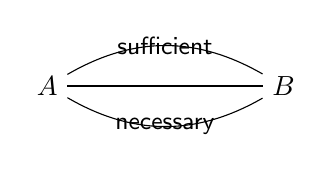
\begin{tikzpicture}
    \node[] (a) at (0,0) {$A$};
    \node[] (b) at (3,0) {$B$};
    \path[every node/.style={font=\sffamily\small}]
    (a) edge node {} (b)
    (b) edge[bend left] node {necessary} (a)
    (a) edge[bend left] node {sufficient} (b);
\end{tikzpicture}
\caption{The antecedent of a material conditional is a sufficient condition for the consequent, while the consequent is a necessary condition for the antecedent.}
\label{fig:necessary_and_sufficient}
\end{figure}


\section{Combining negation with conjunction and disjunction}

Tricky things happen when you combine a negation with a conjunction or disjunction, so it is worth taking a closer look here. Consider these sentences

\begin{description}
\item[\ex{or3}] Either you will not have soup, or you will not have salad.
\item[\ex{or4}] You will have neither soup nor salad.
\end{description}

We let $S_1$ mean that you get soup and $S_2$ mean that you get salad. Sentence \ref{or3} can be paraphrased in this way: ``Either \emph{it is not the case that} you get soup, or \emph{it is not the case that} you get salad.'' Translating this requires both disjunction and negation. It becomes $\lnot S_1 \lor \lnot S_2$.

Sentence \ref{or4} also requires negation. It can be paraphrased as, ``\emph{It is not the case that} either you get soup or you get salad.'' We need some way of indicating that the negation does not just negate the right or left disjunct, but rather negates the entire disjunction. In order to do this, we put parentheses around the disjunction: ``It is not the case that $(S_1 \lor S_2)$.'' This becomes simply $\lnot (S_1 \lor S_2)$. Notice that the parentheses are doing important work here. The sentence $\lnot S_1 \lor S_2$ would mean ``Either you will not have soup, or you will have salad.''

Something similar happens with negation and conjunction. Consider these sentences

\begin{description}
\item[\ex{notand1}] You can't have soup and you can't have salad.
\item[\ex{notand2}] You can't have both soup and salad.
\end{description}

In sentence \ref{notand1}, the two parts of the sentence are negated individually. We would translate it into SL like this: $\lnot S_1 \land $\lnot$ S_2$. In sentence \ref{notand2}, the negation applies to soup and salad taken together. You are allowed to have soup only, or salad only. You just can't have both together. We would translate sentence \ref{notand2} like this: $\lnot(S_1 \land S_2)$.

You can combine disjunction, conjunction, and negation to represent the exclusive or, as in this sentence.

\begin{description}
\item[\ex{or.xor}] You get either soup or salad, but not both.
\end{description}

Remember on page \pageref{def:inclusive_or}, we said that the $\lor$ in SL represented an inclusive or. It said ``this or that or both.'' If we want to represent an exclusive or, we need to combine disjunction, conjuction and negation. We can break the sentence into two parts. The first part says that you get one or the other. We translate this as $(S_1 \lor S_2)$. The second part says that you do not get both. We can paraphrase this as ``It is not the case both that you get soup and that you get salad.'' Using both negation and conjunction, we translate this as $\lnot(S_1 \land S_2)$. Now we just need to put the two parts together. As we saw above, ``but'' can usually be translated as a conjunction. Sentence \ref{or.xor} can thus be translated as $(S_1 \lor S_2) \land \lnot(S_1 \land S_2)$.



\section{Recursive Syntax for SL}\label{recursive_syntax_for_SL}

The previous two sections gave you a rough, informal sense of how to create sentences in SL. If I give you an English sentence like ``Grass is either green or brown,'' you should be able to write a corresponding sentence in SL: ``$A \lor B$.'' In this section we want to give a more precise definition of a sentence in SL.  When we defined sentences in English, we did so using the concept of truth: Sentences were units of language that can be true or false. (See page \pageref{def:statement}.) In SL, it is possible to define what counts as a sentence without talking about truth. Instead, we can just talk about the structure of the sentence. This is one respect in which a formal language like SL is more precise than a natural language like English.

\newglossaryentry{syntax}
{
name=syntax,
description={The structure of a bit of language, considered without reference to truth, falsity, or meaning.}
}

\newglossaryentry{semantics}
{
name=semantics,
description={The meaning of a bit of language is its meaning, including truth and falsity.}
}

The structure of a sentence in SL considered without reference to truth or falsity is called its syntax. More generally \textsc{\gls{syntax}} \label{def:syntax} refers to the study of the properties of language that are there even when you don't consider meaning. Whether a sentence is true or false is considered part of its meaning. In this chapter, we will be giving a purely syntactical definition of a sentence in SL.  The contrasting term is \textsc{\gls{semantics}} \label{def:semantics} the study of aspects of language that relate to meaning, including truth and falsity. (The word ``semantics'' comes from the Greek word for ``mark'')

\newglossaryentry{object language}
{
name=object language,
description={A language that is constructed and studied by logicians. In this textbook, the object languages are SL and QL.
}


\newglossaryentry{metalanguage}
{
name=metalanguage,
description={The language logicians use to talk about the object language. In this textbook, the metalanguage is English, supplemented by certain symbols like metavariables and technical terms like ``valid.''}
}

If we are going to define a sentence in SL just using syntax, we will need to carefully distinguish SL from the language that we use to talk about SL. When you create an artificial language like SL, the language that you are creating is called the \textsc{\gls{object language}}. \label{def:object_language} The language that we use to talk about the object language is called the \textsc{\gls{metalanguage}}. \label{def:metalanguage} Imagine building a house. The object language is like the house itself. It is the thing we are building. While you are building a house, you might put up scaffolding around it. The scaffolding isn't part of the the house. You just use it to build the house. The metalanguage is like the scaffolding.

The object language in this chapter is SL. For the most part, we can build this language just by talking about it in ordinary English. However we will also have to build some special scaffolding that is not a part of SL, but will help us build SL. Our metalanguage will thus be ordinary English plus this scaffolding.

\newglossaryentry{metavariables}
{
name=metavariables,
description={A variable in the metalanguage that can represent any sentence in the object language.}
}

An important part of the scaffolding are the \textsc{\gls{metavariables}} \label{def:metavariables} These are the fancy script letters we have been using in the characteristic truth tables for the connectives: $\mathcal{A}$, $\mathcal{B}$, $\mathcal{C}$, etc. These are letters that can refer to any sentence in SL. They can represent sentences like $P$ or $Q$, or they can represent longer sentences, like $(((A \lor B) \land G) \onlyif (P \iff Q))$.
Just as the sentence letters $A$, $B$, etc. are variables that range over any English sentence, the metavariables $\mathcal{A}$, $\mathcal{B}$, etc. are variables that range over any sentence in SL, including the sentence letters $A$, $B$, etc.

As we said, in this chapter we will give a syntactic definition for ``sentence of SL.'' The definition itself will be given in mathematical English, the metalanguage. Table \ref{tab:basic_elements_of_SL} gives the basic elements of SL.


\begin{table}
\begin{tabu}{X[2] X[4]}
\textbf{Element} & \textbf{Symbols} \\
sentence letters & $A,B,C,\ldots,Z,A_1, B_1,Z_1,A_2,A_{25},J_{375},\ldots$ \\
connectives      & $\lnot,\land,\lor,\onlyif,\iff$ \\
parentheses      & $(,)$ \\
\end{tabu}
\caption{The basic elements of SL} \label{tab:basic_elements_of_SL}
\end{table}


Most random combinations of these symbols will not count as sentences in SL. Any random connection of these symbols will just be called a ``string'' or ``expression'' Random strings only become meaningful sentences when the are structured according to the rules of syntax. We saw from the earlier two sections that individual sentence letters,  like $A$ and $G_{13}$ counted as sentences. We also saw that we can put these sentences together using connectives so that  $\lnot A$ and $\lnot G_{13}$ is a sentence.  The problem is, we can't simply list all the different sentences we can put together this way, because there are infinitely many of them. Instead, we will define a sentence in SL by specifying the process by which they are constructed.

Consider negation: Given any sentence $\mathcal{A}$ of SL, $\lnot\mathcal{A}$ is a sentence of SL. It is important here that $\mathcal{A}$ is not the sentence letter $A$. Rather, it is a metavariable: part of the metalanguage, not the object language. Since $\mathcal{A}$ is not a symbol of SL, $\lnot\mathcal{A}$ is not an expression of SL. Instead, it is an expression of the metalanguage that allows us to talk about infinitely many expressions of SL: all of the expressions that start with the negation symbol.

\newglossaryentry{sentence of SL}
{
name=sentence of SL,
description={A string of symbols in SL that can be built up using according to the recursive rules given on page} % }
}

We can say similar things for each of the other connectives. For instance, if $\mathcal{A} and \mathcal{B}$ are sentences of SL, then $(\mathcal{A}\land\mathcal{B})$ is a sentence of SL. Providing clauses like this for all of the connectives, we arrive at the following formal definition for a \textsc{\gls{sentence of SL}}: \label{def:sentence_of_SL}

\begin{enumerate}
\item Every atomic sentence is a sentence.
\item If $\mathcal{A}$ is a sentence, then $\lnot\mathcal{A}$ is a sentence of SL.
\item If $\mathcal{A}$ and $\mathcal{B}$ are sentences, then $(\mathcal{A}\land\mathcal{B})$ is a sentence.
\item If $\mathcal{A}$ and $\mathcal{B}$ are sentences, then $(\mathcal{A}\lor\mathcal{B})$ is a sentence.
\item If $\mathcal{A}$ and $\mathcal{B}$ are sentences, then $(\mathcal{A}\onlyif\mathcal{B})$ is a sentence.
\item If $\mathcal{A}$ and $\mathcal{B}$ are sentences, then $(\mathcal{A}\iff\mathcal{B})$ is a sentence.
\item All and only sentences of SL can be generated by applications of these rules.
\end{enumerate}

We can apply this definition to see whether an arbitrary string is a sentence. Suppose we want to know whether or not $\lnot\lnot\lnot D$ is a sentence of SL.
Looking at the second clause of the definition, we know that $\lnot\lnot\lnot D$ is a sentence \emph{if} $\lnot\lnot D$ is a sentence.
So now we need to ask whether or not $\lnot\lnot D$ is a sentence.
Again looking at the second clause of the definition, $\lnot\lnot D$ is a sentence \emph{if} $\lnot D$ is.
Again, $\lnot D$ is a sentence \emph{if} $D$ is a sentence.
Now $D$ is a sentence letter, an atomic sentence of SL, so we know that $D$ is a sentence by the first clause of the definition.
So for a compound formula like $\lnot\lnot\lnot D$, we must apply the definition repeatedly. Eventually we arrive at the atomic sentences from which the sentence is built up.

\newglossaryentry{recursive definition}
{
name=recursive definition,
description={A definition that defines a term by identifying base class and rules for extending that class. Also called an ``inductive definition.''}
}

Definitions like this are called recursive. \textsc{\Glspl{recursive definition}}\label{def:recursive_definition} begin with some specifiable base elements and define ways to indefinitely compound the base elements. Just as the recursive definition allows complex sentences to be built up from simple parts, you can use it to decompose sentences into their simpler parts. To determine whether or not something meets the definition, you may have to refer back to the definition many times. Recursive definitions are also sometimes called ``inductive definitions.''

\newglossaryentry{sentential logic}
{
name=sentential logic,
description={A system of logic in which statements can be defined using a recursive definition with only sentences in the base class.}
}


We are now in a position to define what it means for a system of logic to be a system of sentential logic. A \textsc{\gls{sentential logic}} \label{def:sentential_logic} is a system of logic in which statements can be defined using a recursive definition with only sentences in the base class. This book defines on system of sentential logic, which we call SL. Other books use other systems.


\newglossaryentry{scope}
{
name=scope,
description={The sentences that are joined by a connective. These are the sentences the connective was applied to when the sentence was assembled using a recursive definition.}
}

When you use a connective to build a longer sentence from shorter ones, the shorter sentences are said to be in the \textsc{\gls{scope}} \label{def:scope} of the connective. So in the sentence $(A \land B) \onlyif C$, the scope of the connective $\onlyif$ includes $(A \land B)$ and C. In the sentence $\lnot(A \land B)$ the scope of the $\lnot$ is $(A \land B)$. On the other hand, in the sentence $\lnot A \land B$ the scope of the $\lnot$ is just $A$.

\newglossaryentry{main connective}
{
name=main connective,
description={The last connective that you add when you assemble a sentence using the recursive definition.}
}

The last connective that you add when you assemble a sentence using the recursive definition is the \textsc{\gls{main connective}} \label{def:main_connective} of that sentence. For example: The main logical operator of $\lnot (E \lor (F \onlyif G))$ is negation, $\lnot$. The main logical operator of $(\lnot E \lor (F \onlyif G))$ is disjunction, $\lor$. The main connective of any sentence will have all the rest of the sentence in its scope.

\newglossaryentry{unique readability}
{
name=unique readability,
description={A property of formal languages which is present when each well-formed formula is the product of a unique process of recursive construction.}
}

Because statement in our language is defined recursively, we can say it is ``uniquely readable.'' \textsc{\Gls{unique readability}}\label{def:unique_readability} is a property of formal languages which is present when each well-formed formula can only be constructed in a single way. Every process of building up a sentence recursively yields a unique sentence, and every sentence is the product of a unique process of recursive definitions. This means that in an important sense our language SL is free of ambiguity, which is a key goal in the construction of any formal language. Every sentence in SL will have a unambiguous main connective and every connective in a sentence will have an unambiguous scope. This makes logicians happy.


%The recursive structure of sentences in SL will be important when we consider the circumstances under which a particular sentence would be true or false. The sentence $\lnot $\lnot$ \lnot D$ is true if and only if the sentence $\lnot $\lnot$ D$ is false, and so on through the structure of the sentence until we arrive at the atomic components: $\lnot $\lnot$ \lnot D$ is true if and only if the atomic sentence $D$ is false. We will return to this point in the next chapter.
%restore when you restore the recursive part of chap. 3.

\section{Notational conventions}
\label{SLconventions}
A sentence like $(Q \land R)$ must be surrounded by parentheses, because we might apply the definition again to use this as part of a more complicated sentence. If we negate $(Q \land R)$, we get $\lnot(Q \land R)$. If we just had $Q \land R$ without the parentheses and put a negation in front of it, we would have $\lnot Q \land R$. It is most natural to read this as meaning the same thing as $(\lnot Q \land R)$, something very different than $\lnot(Q\land R)$. The sentence $\lnot(Q \land R)$ means that it is not the case that both $Q$ and $R$ are true; $Q$ might be false or $R$ might be false, but the sentence does not tell us which. The sentence $(\lnot Q \land R)$ means specifically that $Q$ is false and that $R$ is true. As such, parentheses are crucial to the meaning of the sentence.

So, strictly speaking, $Q \land R$ without parentheses is \emph{not} a sentence of SL. When using SL, however, we will often be able to relax the precise definition so as to make things easier for ourselves. We will do this in several ways.

First,  we understand that $Q \land R$ means the same thing as $(Q \land R)$. As a matter of convention, we can leave off parentheses that occur \emph{around the entire sentence}.

Second, it can sometimes be confusing to look at long sentences with many nested pairs of parentheses. We adopt the convention of using square brackets [ and ] in place of parentheses. There is no logical difference between $(P\lor Q)$ and $[P\lor Q]$, for example. The unwieldy sentence
$$(((H \onlyif I) \lor (I \onlyif H)) \land (J \lor K))$$
could be written in this way:
$$\bigl[(H \onlyif I) \lor (I \onlyif H)\bigr] \land (J \lor K)$$


Third, we will sometimes want to translate the conjunction of three or more sentences. For the sentence ``Alice, Bob, and Candice all went to the party,'' suppose we let $A$ mean ``Alice went,'' $B$ mean ``Bob went,'' and $C$ mean ``Candice went.'' The definition only allows us to form a conjunction out of two sentences, so we can translate it as $(A \land B) \land C$ or as $A \land (B \land C)$. There is no reason to distinguish between these, since the two translations are logically equivalent. There is no logical difference between the first, in which $(A \land B)$ is conjoined with $C$, and the second, in which $A$ is conjoined with $(B \land C)$.  So we might as well just write $A \land B \land C$. As a matter of convention, we can leave out parentheses when we conjoin three or more sentences.

Fourth, a similar situation arises with multiple disjunctions. ``Either Alice, Bob, or Candice went to the party'' can be translated as $(A \lor B) \lor C$ or as $A \lor (B \lor C)$. Since these two translations are logically equivalent, we may write $A \lor B \lor C$.

These latter two conventions only apply to multiple conjunctions or multiple  disjunctions. If a series of connectives includes both disjunctions and conjunctions, then the parentheses are essential; as with $(A \land B) \lor C$ and $A \land (B \lor C)$. The parentheses are also required if there is a series of conditionals or biconditionals; as with $(A \onlyif B) \onlyif C$ and $A \iff (B \iff C)$.

We have adopted these four rules as notational conventions, not as changes to the definition of a sentence. Strictly speaking, $A \lor B \lor C$ is still not a sentence. Instead, it is a kind of shorthand. We write it for the sake of convenience, but we really mean the sentence $(A \lor (B \lor C))$.

If we had given a different definition for a sentence, then these could count as sentences. We might have written rule 3 in this way: ``If $\mathcal{A}, \mathcal{B}, \ldots \mathcal{Z}$ are sentences, then $(\mathcal{A}\land\mathcal{B}\land\ldots\land\mathcal{Z})$, is a sentence .'' This would make it easier to translate some English sentences, but would have the cost of making our formal language more complicated. We would have to keep the complex definition in mind when we develop truth tables and a proof system. We want a logical language that is expressively simple and allows us to translate easily from English, but we also want a formally simple language. Adopting notational conventions is a compromise between these two desires.


\section*{Key Terms}
\begin{multicols}{2}
\begin{sortedlist}
\sortitem{Sentence letter}{}
\sortitem{Symbolization key}{}
\sortitem{Atomic sentence}{}
\sortitem{Sentential connective}{}
\sortitem{Negation}{}
\sortitem{Conjunction}{}
\sortitem{Conjunct}{}
\sortitem{Disjunction}{}
\sortitem{Disjunct}{}
\sortitem{Conditional}{}
\sortitem{Antecedent}{}
\sortitem{Consequent}{}
\sortitem{Biconditional}{}
\sortitem{Syntax}{}
\sortitem{Semantics}{}
\sortitem{Object language}{}
\sortitem{Metalanguage}{}
\sortitem{Metavariables}{}
\sortitem{Sentence of SL}{}
\sortitem{Main connective}{}
\sortitem{Recursive definition}{}
\sortitem{Scope}{}
\sortitem{Nonlogical symbol}{}
\sortitem{Logical constant}{}
\sortitem{Exclusive or}{}
\sortitem{Inclusive or}{}
\sortitem{Necessary condition}{}
\sortitem{Sufficient condition}{}
\sortitem{Translation key}{}
\end{sortedlist}
\end{multicols}

    \chapter{Truth Tables}\label{ch:truth_tables}
\markright{Chapter \ref{ch:truth_tables}: Truth Tables}

This chapter introduces a way of evaluating sentences and arguments of SL called the truth table method. As we shall see, the truth table method is \emph{semantic} because it involves one aspect of the meaning of sentences, whether those sentences are true or false. As we saw on page \pageref{def:semantics}, semantics is the study of aspects of language related to meaning, including truth and falsity. Although it can be laborious, the truth table method is a purely mechanical procedure that requires no intuition or special insight. When we get to Chapter \ref{chap:semantics_for_ql},we will provide a parallel semantic method for QL; however, this method will not be purely mechanical.

\section{Basic Concepts}

\newglossaryentry{logical constant}
{
name=logical constant,
description={A symbol whose meaning is fixed by a formal language. Sometimes these are just called ``logical symbols.'' They are contrasted with \textsc{non-logical symbols}.}
}

\newglossaryentry{nonlogical symbol}
{
name=nonlogical symbol,
description={A symbol whose meaning is not fixed by a formal language.}
}



In the previous chapter, we said that a formal language is built from two kinds of elements: logical constants and nonlogical symbols. The \textsc{\glspl{logical constant}}\label{def:logical_constant} have their meaning fixed by the formal language, while the \textsc{\glspl{nonlogical symbol}} \label{def:nonlogical_symbol} get their meaning in the symbolization key. The logical constants in SL are the sentential connectives and the parentheses, while the nonlogical symbols are the sentence letters.

\newglossaryentry{interpretation}
{
name=interpretation,
description={A correspondence between nonlogical symbols of the object language and elements of some other language or logical structure.}
}

When we assign meaning to the nonlogical symbols of a language using a dictionary, we say we are giving an ``interpretation'' of the language. More formally an \textsc{\gls{interpretation}\label{def:interpretation}} of a language is a correspondence between elements of the object language and elements of some other language or logical structure. The symbolization keys we defined in Chapter \ref{chap:SL} (p. \pageref{def:translation_key}) are one sort of interpretation. Fancier languages will have more complicated kinds of interpretations.

\newglossaryentry{truth value}
{
  name=truth value,
  description={The status of a statement with relationship to truth. For  this textbook, this means the status of a statement as true or false}
}

The truth table method will also involve giving an interpretation of sentences, but they will be much simpler than the translation keys we used in Chapter \ref{chap:SL}. We will not be concerned with what the individual sentence letters mean. We will only care whether they are true or false. In other words, our interpretations will assign \glspl{truth value} to the sentence letters. (See page \pageref{def:Truth_value}.)

\newglossaryentry{truth-functional connective}
{
name=truth-functional connective,
description={an operator that builds larger sentences out of smaller ones and fixes the truth value of the resulting sentence based only on the truth value of the component sentences.}
}

We can get away with only worrying about the truth values of sentence letters because of the way that the meaning of larger sentences is generated by the meaning of their parts. Any larger sentence of SL is composed of atomic sentences with sentential connectives. The truth value of the compound sentence depends only on the truth value of the atomic sentences that it comprises. In order to know the truth value of $D\iff E$, for instance, you only need to know the truth value of $D$ and the truth value of $E$. Connectives that work in this way are called truth functional. More technically, we define a \textsc{\gls{truth-functional connective}} \label{def:truth-functional_connective}as an operator that builds larger sentences out of smaller ones, and fixes the truth value of the resulting sentence based only on the truth value of the component sentences.

\newglossaryentry{truth assignment}
{
name=truth assignment,
description={A function that maps the sentence letters in SL onto truth values.}
}

Because all of the logical symbols in SL are truth functional, we can study the the semantics of SL looking only at truth and falsity. If we want to know about the truth of the sentence $A \land B$, the only thing we need to know is whether $A$ and $B$ are true. It doesn't actually matter what else they mean. So if $A$ is false, then $A \land B$ is false no matter what false sentence $A$ is used to represent. It could be ``I am the Pope'' or ``Pi is equal to 3.19.'' The larger sentence $A \land B$ is still false. So to give an interpretation of sentences in SL, all we need to do is create a truth assignment. A \textsc{\gls{truth assignment}} \label{def:truth_assignment} is a function that maps the sentence letters in SL onto our two truth values. In other words, we just need to assign Ts and Fs to all our sentence letters.

It is worth knowing that most languages are not built only out of truth functional connectives. In English, it is possible to form a new sentence from any simpler sentence $\mathcal{X}$ by saying ``It is possible that $\mathcal{X}$.'' The truth value of this new sentence does not depend directly on the truth value of $\mathcal{X}$. Even if $\mathcal{X}$ is false, perhaps in some sense $\mathcal{X}$ \emph{could} have been true---then the new sentence would be true. Some formal languages, called \emph{modal logics}, have an operator for possibility. In a modal logic, we could translate ``It is possible that $\mathcal{X}$'' as {\large $\diamond$}$\mathcal{X}$. However, the ability to translate sentences like these comes at a cost: The {\large $\diamond$} operator is not truth-functional, and so modal logics are not amenable to truth tables.

\section{Complete Truth Tables}

In the last chapter we introduced the characteristic truth tables for the different connectives. To put them all in one place, the truth tables for the connectives of SL are repeated in Table \ref{tab:CharacteristicTTs}. On the left is the truth table for negation, and on the right is the truth table for the other four connectives. Notice that the truth table for the negation is shorter than the other table. This is because there is only one metavariable here, $\mathcal{A}$, which can either be true or false. The other connectives involve two metavariables, which give us four possibilities of true and false. The columns to the left of the double line in these tables are called the reference columns. They just specify the truth values of the individual sentence letters. Each row of the table assigns truth values to all the variables. Each row is thus a truth assignment---a kind of interpretation---for that sentence. Because the full table gives all the possible truth assignments for the sentence, it gives all the possible interpretations of it.


\begin{table}
\begin{center}
\begin{longtabu}{cccc|c||c|c|c|c}
\multicolumn{1}{r||}{$\mathcal{A}$}&$\lnot\mathcal{A}$ & & $\mathcal{A}$ & $\mathcal{B}$ & $\mathcal{A}\land\mathcal{B}$ & $\mathcal{A}\lor\mathcal{B}$ & $\mathcal{A}\onlyif\mathcal{B}$ & $\mathcal{A}\iff\mathcal{B}$\\
\cline{1-2} \cline{4-9}
\multicolumn{1}{r||}{T}	&	F	&	& T & T & T & T & T & T \\
\multicolumn{1}{r||}{F}	&	T	&	& T & F & F & T & F & F \\
	                    &		&	& F & T & F & T & T & F \\
	                    &		&	& F & F & F & F & T & T \\
\end{longtabu}
\end{center}
\caption{The characteristic truth tables for the connectives of SL.}
\label{tab:CharacteristicTTs}
\end{table}

The truth table of sentences that contain only one connective is given by the characteristic truth table for that connective. So the truth table for the sentence $P \land Q$ looks just like the characteristic truth table for $\land$, with the sentence letters $P$ and $Q$ substituted in. The truth tables for more complicated sentences can simply be built up out of the truth tables for these basic sentences. Consider the sentence $(H\land I)\onlyif H$. This sentence has two sentence letters, so we can represent all the possible truth assignments using a four line truth table. We can start by writing out all the possible combinations of true and false for $H$ and $I$ in the reference columns. We then copy the truth values for the sentence letters and write them underneath the letters in the sentence.

\begin{center}
\begin{tabu}{c|c||@{\TTon}*{5}{c}@{\TToff}}
$H$ & $I$ & $(H$ & $\land$ & $I)$ & $\onlyif$ & $H$ \\
\hline
 T & T & T & & T & & T\\
 T & F & T & & F & & T\\
 F & T & F & & T & & F\\
 F & F & F & & F & & F
\end{tabu}
\end{center}

Now consider just one part of the sentence above, the subsentence $H\land I$. This is a conjunction $\mathcal{A}\land\mathcal{B}$ with $H$ as $\mathcal{A}$ and with $I$ as $\mathcal{B}$. $H$ and $I$ are both true on the first row. Since a conjunction is true when both conjuncts are true, we write a T underneath the conjunction symbol. We continue for the other three rows and get this:

\begin{center}
\begin{tabu}{c|c||ccccc}%{c|c||@{\TTon}*{5}{c}@{\TToff}}
\multicolumn{1}{r}{} &\multicolumn{1}{r}{} & \multicolumn{3}{c}{$(\mathcal{A}\land\mathcal{B})$} & & \\
\multicolumn{1}{r}{} &\multicolumn{1}{r}{} & \multicolumn{3}{c}{\downbracefill} & & \\
$H$	&	$I$	&	$(H$	&$\land$	&	$I)$	&	$\onlyif$	&	$H$\\
\hline
 T & T & T & \TTbf{T} & T & & T\\
 T & F & T & \TTbf{F} & F & & T\\
 F & T & F & \TTbf{F} & T & & F\\
 F & F & F & \TTbf{F} & F & & F\\
\end{tabu}
\end{center}

Next we need to fill in the final column under the conditional. The conditional is the main connective of the sentence, so the whole sentence is of the form $\mathcal{A}\onlyif\mathcal{B}$ with $(H \land I)$ as $\mathcal{A}$ and with $H$ as $\mathcal{B}$. So to fill the final column, we just need to look at the characteristic truth table for the conditional. For the first row, the sentence $(H \land I)$ is true and the sentence $H$ is also true. The truth table for he conditional tells us this means that the whole sentence is true. Filling out the rest of the column gives us this:

\begin{center}
\begin{tabu}{c|c||ccccc}%{c|c||@{\TTon}*{5}{c}@{\TToff}}
\multicolumn{1}{r}{} &\multicolumn{1}{r}{} & \multicolumn{3}{c}{\mathcal{A}} & \onlyif & \mathcal{B} \\
\multicolumn{1}{r}{} &\multicolumn{1}{r}{} & \multicolumn{3}{c}{\downbracefill}	& \downbracefill & \downbracefill \\
$H$ & $I$ & $(H$ & $\land$ & $I)$ & $\onlyif$ & $H$\\
\hline
 T & T & T & {T} & T &\TTbf{T} & T\\
 T & F & T & {F} & F &\TTbf{T} & T\\
 F & T & F & {F} & T &\TTbf{T} & F\\
 F & F & F & {F} & F &\TTbf{T} & F\\
\end{tabu}
\end{center}

The column of Ts underneath the conditional tells us that the sentence $(H \land I)\onlyif H$ is true regardless of the truth values of $H$ and $I$. They can be true or false in any combination, and the compound sentence still comes out true. It is crucial that we have considered all of the possible combinations. If we only had a two-line truth table, we could not be sure that the sentence was not false for some other combination of truth values.

In this example, the script letters over the table have just been there to indicate how the columns get filled in. We won't need them in the final product. Also, the reference columns are redundant with the columns under the individual sentence letters, so we can eliminate those as well. Most of the time, when you see truth tables, we will just write them out this way:
\begin{center}
\begin{tabu}{ccccc}
$(H$	&	\land	&	$I)$	& \onlyif	\tikz[overlay, shift={(0ex,-27pt)}, gray] \draw (0pt,0pt) ellipse (2ex and 44pt);			&$H$\\
\hline
T 		& 	{T} 	& 	T 		& T 	& T\\
T 		& 	{F} 	& 	F 		& T 	& T\\
F 		& 	{F} 	&	T 		& T 	& F\\
F 		& 	{F} 	& 	F 		& T 	& F
\end{tabu}
\end{center}
\label{tautology3.1}

The truth value of the sentence on each row is just the column underneath the \emph{main connective} (see p. \pageref{def:main_connective}) of the sentence, in this case, the column underneath the conditional.

\newglossaryentry{complete truth table}
{
name=complete truth table,
description={A table that gives all the possible interpretations for a sentence or set of sentences in SL.}
}

A \textsc{\gls{complete truth table}} \label{def:complete_truth_table} is a table that gives all the possible interpretations for a sentence or set of sentences in SL. It has a row for each possible assignment of T and F to all of the sentence letters. The size of the complete truth table depends on the number of different sentence letters in the table. A sentence that contains only one sentence letter requires only two rows, as in the characteristic truth table for negation. This is true even if the same letter is repeated many times, as in this sentence: $$[(C\iff C) \onlyif C] \land \lnot(C \onlyif C).$$ The complete truth table requires only two lines because there are only two possibilities: $C$ can be true, or it can be false. A single sentence letter can never be marked both T and F on the same row. The truth table for this sentence looks like this:
\begin{center}
\begin{tabu}{cccccccccc}%{c@{\TTon}*{13}{c}@{\TToff}}
[($C$	&\iff	&	$C)$	&	\onlyif	&	$C]$	&	\land	\tikz[overlay, shift={(-1ex,-12pt)}, gray] \draw (0pt,0pt) ellipse (2ex and 27pt);		&\lnot	&	$(C$	&	\onlyif	&	$C)$\\
\hline
	T 	&  T  	& 	T 		&  T  		& 	T 		&	F	&  F		& T 		&  T 		& T \\
	F 	&  T  	& 	F		&  F  		&	F 		&	F	&  F		& F 		&  T  		& F \\
\end{tabu}
\end{center}
\label{contradiction3.1}
Looking at the column underneath the main connective, we see that the sentence is false on both rows of the table; i.e., it is false regardless of whether $C$ is true or false.

A sentence that contains two sentence letters requires four lines for a complete truth table, as we saw above in the table for $(H \land I)\onlyif I$.

A sentence that contains three sentence letters requires eight lines, as in this example. Here the reference columns are included so you can see how to arrange the truth values for the individual sentence letters so that all the possibilities are covered.

\begin{center}
\begin{tabu}{c|c|c|@{\TTon}*{5}{c}@{\TToff}}
$M$	&	$N$	&	$P$	&	$M$	&	\land	\tikz[overlay, shift={(-1.25ex,-52pt)}, gray] \draw (0pt,0pt) ellipse (2ex and 66pt);			&	$(N$	&	\lor	&	$P)$\\
\hline
%           M        &     N   v   P
T		& T 		& T 		& T 		& T & T & T & T\\
T 		& T 		& F 		& T 		& T & T & T & F\\
T 		& F 		& T 		& T 		& T & F & T & T\\
T 		& F 		& F 		& T 		& F & F & F & F\\
F 		& T 		& T 		& F 		& F & T & T & T\\
F 		& T 		& F 		& F 		& F & T & T & F\\
F 		& F 		& T 		& F 		& F & F & T & T\\
F 		& F 		& F 		& F 		& F & F & F & F
\end{tabu}
\end{center}
\label{contingentsentence3.1}
From this table, we know that the sentence $M\land(N\lor P)$ might be true or false, depending on the truth values of $M$, $N$, and $P$.

A complete truth table for a sentence that contains four different sentence letters requires 16 lines. For five letters, 32 lines are required. For six letters, 64 lines, and so on. To be perfectly general: If a complete truth table has $n$ different sentence letters, then it must have $2^n$ rows.

By convention, the reference columns are filled in with the right most row alternating Ts and Fs. The next column over alternates sets of two Ts and two Fs. For the third column from the right, you have sets of four Ts and four Fs. This continues until you reach the leftmost column, which will always have the top have all Ts and the bottom half all Fs. This convention is completely arbitrary. There are other ways to be sure that all the possible combinations are covered, but everything is easier if we all stick to the same pattern.

\section*{Key Terms}
\begin{multicols}{2}
\begin{sortedlist}
\sortitem{Semantically contingent in SL}{}
\sortitem{Semantically logically equivalent in SL}{}
\sortitem{Semantically consistent in SL}{}
\sortitem{Semantically valid in SL}{}
\sortitem{Semantic contradiction in SL}{}
\sortitem{Semantic tautology in SL}{}
\sortitem{Complete truth table}{}
\sortitem{Truth assignment}{}
\sortitem{Truth-functional connective}{}
\sortitem{Nonlogical symbol}{}
\sortitem{Logical constant}{}
\sortitem{Interpretation}{}
\end{sortedlist}
\end{multicols}

    %\include{tex/32-naturaldeduction}
    %\include{tex/33-existentialgraphs}

%\part{Predicate \& Quantifier Logic}\label{part:pred_logic}
    %\include{tex/40-predicate}
    %\include{tex/41-semanticsforql}
    %\include{tex/42-proofsinql}
    %\include{tex/43-quantification}
    %\include{tex/44-alternativequantifiers}

%\part{Modal Logic}\label{part:modal_logic}
    %\include{tex/45-basicmodality}
    %\include{tex/46-kripkeframes}
    %\include{tex/47-accessibility}
    %\include{tex/48-actuality}
    %\include{tex/49-alternativemodals}

\part{Inductive Logic and Scientific Reasoning}\label{part:inductive_scientific}
    \chapter{What are Induction and Scientific Reasoning?}
\markright{Chap \ref{ch:inductionandscience}: Induction and Science}
\label{ch:inductionandscience}
\setlength{\parindent}{1em}

\section{Introduction}

Earlier in our discussion of logic we made the distinction between deductive and inductive forms of inference. Recall that while deduction and deductive inferences are inferences that attempt to guarantee the truth of the conclusion on the basis of the premises, induction and inductive inferences attempt something less ambitious. In short, induction is any form of inference in which the premises are not intended to logically entail or guarantee their conclusion, but merely to provide some support to it. In this part of the book we'll be examining inductive logic in more detail, with special attention paid to a rigorous form of inductive reasoning as applied in the sciences.

Before we begin, you may be asking yourself, ``Why should we care about inductive reasoning at all?'' After all, deductive inferences \emph{guarantee} their conclusions and that's the best kind of evidential support you could hope for! Shouldn't we just spend all of our time focusing on making deductive inferences?

This is a reasonable complaint, and one worth taking seriously. While valid deduction is the absolute best form of evidential support a conclusion can receive, we should care about induction as well, for at least the following reasons.

First, many of the inferences people make every day are inductive, not deductive. Consider just the inferences you make when you go to the refrigerator to make a sandwich. Suppose you reason as follows:

\begin{kormanize}
\premise{Yesterday I bought sandwich ingredients and put them in my refrigerator.}
\conclusion{So, today there are sandwich ingredients in my refrigerator.}
\end{kormanize}

Of course, the conclusion isn't entailed by that premise. Perhaps your roommate ate all of the cold cuts, cheese, and vegetables that you bought at the store yesterday in a late night binge. If so, then the conclusion obviously would not follow from the premise. Okay, but we can deal with this by adding another premise, such as ``No one has touched my sandwich ingredients since I put them in the refrigerator.'' Still, the conclusion does not follow \emph{deductively} from these premises since it could be that while no one has touched them the power went out in your building and all of the food in your refrigerator has gone bad!

We could go on and on like this, but the point is that most of the inferences we make are not in the form of a deductively valid argument. We often reason on limited evidence, or via less than valid forms of inference. So it is worthwhile to understand how inductive inference functions.

A second reason to care about inductive inference is that deductive inferences are fundamentally \emph{limited}. By this I mean to emphasize the logician and philosopher C. S. Peirce's term for inductive inference: \textsc{\gls{ampliative logic}}. By ampliative, Peirce meant that the premises `amplify' what can be deductively inferred from them. That is, the premises go beyond their deductive entailments.

\newglossaryentry{ampliative logic}
{
name=Ampliative Logic,
description={Ampliative logic is another term for inductive logic, or a logic the inferences of which do not guarantee or logically entail the truth of the conclusion on the basis of the premises. See also \gls{inductive logic}.}
}

Ampliative inference is just another word for inductive inference, but the point is the same. Inductive inferences tell us something about the world that is not already contained in the premises. For example, consider this classic deductive argument from categorical logic:

\begin{kormanize}
\premise{All dogs like peanut butter.}
\premise{Rose is a dog.}
\conclusion{So, Rose likes peanut butter.}
\end{kormanize}

Now consider that if you \emph{accept} the premises, then there's an important sense in which the conclusion doesn't tell you anything you didn't already know. You haven't learned anything about the world from this argument (assuming you already knew the premises). However, contrast that argument with the following inductive `version': 

\begin{kormanize}
\premise{Most dogs like peanut butter.}
\premise{Rose is a dog.}
\conclusion{So, Rose likes peanut butter.}
\end{kormanize}

Obviously, the conclusion isn't entailed by these premises (the argument isn't valid). However, if you come to know the conclusion on the basis of these premise you \emph{do} learn something new; namely, you learn that Rose is one of the majority of dogs who like peanut butter. 

A final consideration for why induction is important is simply that most scientific inferences are made as inductive, rather than deductive, inferences. The logic of science and statistics is fundamentally inductive, not deductive. To gain a better understanding of science it is extremely important to understand how inductive inference functions.

Before moving on to the next chapters, we'll spend the remainder of this chapter discussing some basic concepts in the history and philosophy of science in order to give some context for later discussions.

\section{Early Scientific Method}

The history of philosophy is the history of science. Aristotle wrote lengthy treatises on the nature of mechanics and dynamics, on biology, geology, and optics. For most of history there was no sharp distinction between the scientist (a term invented by the philosopher and scientist William Whewell in 1833) and the philosopher.

One of the things that characterizes the early development of the scientific method is a commitment to \textsc{\gls{empiricism}}. Empiricism is the view that the only, or perhaps the primary, source of knowledge is sensory evidence or the experience of the senses. This view is contrasted with \textsc{\gls{rationalism}}, which says that the source of knowledge is the internal mechanisms of reason.

\newglossaryentry{empiricism}
{
name=Empiricism,
description={Empiricism is a view in epistemology according to which the only, or perhaps the primary, source of knowledge is sensory evidence or the experience of the senses. See also \gls{rationalism}.}
}

\newglossaryentry{rationalism}
{
name=Rationalism,
description={Rationalism is the view in epistemology that knowledge comes from internal mechanisms of reason or rationality. See also \gls{empiricism}.}
}

Both of these views have had their philosophical defenders and both have a lot of evidence that we can acquire knowledge in the way recommended by the view. Consider, for example, proofs in geometry. The truths of mathematics in general, and geometry in particular, seem to be true no matter what. That is, these truths don't depend on making certain kinds of observations or collecting any evidence. Thus, the rationalists say, truths of this kind of derivable from pure reason. Notice that even though you and I may have made observations of a certain kind in our geometry class in order to come to know these truths, this doesn't undermine the rationalist position that such observations are not \emph{required} in order to know geometric proofs. Strict empiricists, on the other hand, maintain that mathematical \emph{concepts} require some kind of of observation and that a being of pure reason and no senses (if such a thing is possible) would not be able to create these concepts from nothing. 

Which of these views do you find more compelling? Think about where knowledge might come from and what kinds of powers are necessary in order to know things about the world. We'll focus on empiricism for now, but think about the truths of logic and their source. Are these truths the result of sensory observations or reason?

Early empiricists noticed very quickly that there are better and worse ways to observe the world around us. As a result they attempted to develop \emph{methods} that would codify and regulate the best ways to make empirical observations and make inferences on the basis of those observations. This is an ongoing process.

There is no one ``scientific method'' that describes the best way to observe, predict, and model the world. Philosophers of science have been engaged in the centuries-long development of various scientific methods to help us make better inferences. 

Starting with Sir Francis Bacon's \textit{Novum Organum} and Rene Descartes' \textit{Discourse on the Method} and ' \textit{Principles of Philosophy} in the 17th century, philosophers of science have generally agreed that a central feature of science is the development of a \textsc{\gls{hypothesis}}. A hypothesis is simply a proposition that may or may not be true and that is subjected to some form of confirmation or disconfirmation.


\newglossaryentry{hypothesis}
{
name=Hypothesis,
description={A hypothesis is a proposition that may or may not be true and can be subjected to confirmation or disconfirmation.}
}


Bacon's method was to begin with the simplest and most obvious observations and then use these observations to confirm or disconfirm hypotheses at greater levels of generality. Descartes, on the other hand, began by doubting the truth of everything that his senses presented to him and trying to identify hypotheses that could not possibly be doubted (such as the famous \emph{cogito ergo sum}, or ``I think, therefore I am.''). Descartes then used this foundation of indubitable truths to derive more commonplace beliefs.

\section{The Hypothetico-Deductive Model}

The \textsc{\gls{hypothetico-deductive model}} of scientific inference is a proposed logical form of inference that explains how scientific hypotheses can be confirmed or disconfirmed.

\newglossaryentry{hypothetico-deductive model}
{
name=Hypothetico-Deductive Model,
description={}
}

The hypothetico-deductive model is one of the more basic methods common to all scientific disciplines, whether it is economics, physics, or biochemistry. Its application can be divided into four stages:

\begin{enumerate}
\item Identify the hypothesis to be tested.
\item Generate predictions from the hypothesis.
\item Perform experiments to check whether predictions are correct.
\item If the predictions are correct, then the hypothesis is confirmed. Otherwise, the hypothesis is disconfirmed.
\end{enumerate}

Suppose your portable music player fails to switch on. You might then consider the hypothesis that perhaps the batteries are dead. So you decide to test whether this is true. Given this hypothesis you predict that the music player should work properly if you replace the batteries with new ones. So you proceed to replace the batteries, which is the ``experiment'' for testing the prediction. If the player works again, then your hypothesis is confirmed, and so you throw away the old batteries. If the player still does not work, then the prediction is false, and the hypothesis is disconfirmed. So you might reject your original hypothesis and come up with an alternative one to test, e.g. the batteries are ok but your music player is broken.

The example above helps us illustrate a few points about science and the hypothetico-deductive method.

\begin{enumerate}
\item A scientific hypothesis must be testable.
\item Confirmation is not truth.
\item Disconfirmation need not be falsity.
\end{enumerate}

Let's consider these points one by one.

First, notice that for us to apply the hypothetico-deductive method we must be able to test our hypothesis. The hypothetico-deductive method tells us that our hypothesis must be capable of being tested, but the method doesn't tell us (a) how to test our hypothesis or (b) how to distinguish between a testable or untestable hypothesis.

If a hypothesis cannot be tested, we cannot find evidence to show that it is probable or not. In that case it cannot be part of scientific knowledge. Consider the hypothesis that there are ghosts that have no causal efficacy, that we cannot neither see nor interact with, and which can never be detected directly or indirectly. This hypothesis is defined in such a way to exclude the possibility of being tested. It might still be true and there might be such ghosts, but we would never be in a position to know and so this cannot be a scientific hypothesis.

Second, notice that confirming the predictions of a hypothesis increases the probability that a hypothesis is correct. But in itself this does not prove conclusively that the hypothesis is correct.

To see why this is the case, we might represent our reasoning as follows:

\begin{kormanize}
\premise{If H then P.}
\premise{P.}
\conclusion{Therefore H.}
\end{kormanize}

\newglossaryentry{process of confirmation}
{
name=Process of Confirmation,
description={}
}

Here H is our hypothesis ``the batteries are dead", and P is the prediction ``the player will function when the batteries are replaced.'' This pattern of reasoning is of course not valid, since there might be reasons other than H that also bring about the truth of P. For example, it might be that the original batteries are actually fine, but they were not inserted properly. Replacing the batteries would then restore the loose connection. So the fact that the prediction is true does not prove that the hypothesis is true. We need to consider alternative hypotheses and see which is more likely to be true and which provides the best explanation of the prediction. (Or we can also do more testing!)

Finally, consider that disconfirmation is sometimes not enough to demonstrate the falsity of the hypothesis. Very often a hypothesis generates a prediction only when given additional assumptions (auxiliary hypotheses). In such cases, when a prediction fails the hypothesis might still be correct.

Looking back at our example again, when we predict that the player will work again when the batteries are replaced, we are assuming that there is nothing wrong with the player. But it might turn out that this assumption is wrong. In such situations the falsity of the prediction does not logically entail the falsity of the hypothesis. We might depict the situation by this argument : ( H=The batteries are dead, A=The player is not broken.)

\begin{kormanize}
\premise{If both H and A, then P.}
\premise{It is not the case that P.}
\conclusion{Therefore, it is not the case that H.}
\end{kormanize}

This argument is of course not valid. When P is false, what follows is not that H is false, only that the conjunction of H and A is false. So there are three possibilities : (a) H is false but A is true, (b) H is true but A is false, or (c) both H and A are false. So we should argue instead :

\begin{kormanize}
\premise{If both H and A, then P.}
\premise{It is not the case that P.}
\conclusion{Therefore, it is not the case that both H and A are true.}
\end{kormanize}

Returning to our earlier example, if the player still does not work when the batteries are replaced, this does not prove conclusively that the original batteries are not dead. This tells us that when we apply the hypothetico-deductive method, we need to examine the additional assumptions that are invoked when deriving the predictions. If we are confident that the assumptions are correct, then the falsity of the prediction would be a good reason to reject the hypothesis. On the other hand, if the hypothesis we are testing has been extremely successful, then we need to be extremely cautious before we reject a hypothesis on the basis of a single false prediction. These additional assumptions used in testing a hypothesis are known as ``auxiliary hypotheses.''

\newglossaryentry{process of disconfirmation}
{
name=Process of Disconfirmation,
description={}
}

\section{The Demarcation Criterion}

How do we distinguish between a scientific and non-scientific hypothesis? Since the philosopher of science Karl Popper, philosophers have referred to the quality or property that distinguishes between science and non-science as the \textsc{\gls{demarcation criterion}}. According to Popper, the demarcation criterion was that a scientific hypothesis must be \textsc{\gls{falsifiable}}, whereas a pseudoscientific or non-scientific hypothesis was not falsifiable.

\newglossaryentry{demarcation criterion}
{
name=Demarcation Criterion,
description={The demarcation criterion is the feature of a hypothesis that distinguishes it as scientific or non-scientific.}
}

\newglossaryentry{falsifiable}
{
name=Falsifiable,
description={A hypothesis is falsifiable if there is some evidence or observation that would demonstrate that the hypothesis is false.}
}

An example of a falsifiable hypothesis is hypothesis that \text{the Earth is flat}. This hypothesis is falsifiable because it can be subjected to several tests such as measuring the angle of approaching ships, shadows, the position of the moon and its path in the sky in different parts of the Earth, and by launching a rocket and making a direct observation that the Earth is not flat. That the Earth is round is likewise falsifiable because it can be falsified by subjecting it to similar tests. The difference between these hypotheses isn't that one is ``more'' scientific than the other; they are equally scientific according to Popper's criterion.

However, there is one important difference between them: one is false and the other is true! The Earth is round and not flat, and we've subjected these hypotheses to many, many tests that have successfully falsified the flat Earth hypothesis and failed to falsify the round Earth hypothesis.\footnote{The epistemic and logical features are an interesting and growing area of philosophical and psychological research.}

An example of an unfalsifiable hypothesis would be the hypothesis that reading Tarot cards will give you insight into your true purpose in life. You can't know that the hypothesis is \emph{false}, since it is vague and relies on a specific interpretation and value system. Another non-falsifiable hypothesis is that God exists. This hypothesis is consistent with any observation, since if the hypothesis is true then it can be used to explain any outcome.

That these hypotheses are non-scientific doesn't mean they aren't meaningful, interesting, or worthwhile. They may also be true or false. What the demarcation criterion tells us is that these hypotheses aren't scientific or amenable to scientific testing. Many ethical, aesthetic, political, theological, philosophical and moral questions are non-scientific.

An important distinction, and the one that Popper initially set out to establish, is between scientific hypotheses and \textsc{\gls{pseudoscience}}. Pseudoscientific hypotheses are not falsifiable---so, according to Popper, they are non-scientific---but they \emph{claim to be} scientific by adopting certain practices or rhetorical moves that scientists adopt. Typically, a perfectly fine scientific hypothesis---such as the flat Earth hypothesis---will become pseudoscientific when it is not rejected appropriately. By adopting a scientific stance, its defenders can claim a kind of epistemic or logical authority that they do not have. 

For example, it is pseudoscientific to defend the flat Earth hypothesis for seemingly scientific reasons while refusing to acknowledge the enormous body of evidence that the hypothesis is false. Alternatively pseudoscientific hypotheses are defended by conducting flawed experiments that do not establish what they purport to establish. Another example of a pseudoscientific hypothesis is young Earth creationism, which explains the existence of fossils and geological evidence for the age of the Earth by appeal to God or another non-falsifiable hypothesis. 

\newglossaryentry{pseudoscience}
{
name=Pseudoscience,
description={A theory or hypothesis is pseudoscientific when it fails to meet the demarcation criterion but adopts rhetorical or argumentative practices that appear to be scientific.}
}

One of the central philosophical challenges is that it is often unclear from the evidence available whether we should consider an ordinary scientific experiment to have falsified a hypothesis outright, or whether we should reject a different, auxiliary hypothesis. This is something that defenders of pseudoscience will often exploit. For example, antivaccination defenders will explain away the numerous falsifications of their hypothesis that vaccinations cause autism or are laced with deadly toxins by claiming that these studies do not replicate. In fact, replication of experimental results is a serious concern in scientific research and so their concern \emph{seems} scientific. However, the studies that reject antivaccination have been extremely well established and replicated\footnote{See e.g. Taylor et. al 2014 (\href{https://www.ncbi.nlm.nih.gov/pubmed/24814559}{link}) for a recent meta-analysis of this research.} so this concern is unwarranted. But knowing when we should reject a hypothesis is a topic of ongoing debate in the philosophy of science.

\section{When should we reject a hypothesis?}

When a hypothesis makes a false prediction, sometimes it can be difficult to know whether we should reject the hypothesis or whether there is something wrong with the auxiliary hypotheses. For example, astronomers in the 19th century found that Newtonian physics could not fully explain planet Mercury's orbit. It turns out that this is because Newtonian physics makes some incorrect assumptions about the structure of space and time, and you need relativity to give a more accurate prediction of the orbit. However, when astronomers discovered Uranus in 1781, they also found out that its orbit was different from the predictions of Newtonian physics. But then scientists realized that it could be explained if there was an additional planet which affected Uranus, and Neptune was subsequently discovered as a result.

Thus, in the case of Mercury's orbit the theory of Newtonian mechanics was falsified and the behavior of the orbit was only explained once we developed relativity theory. However, in the case of Uranus's orbit an auxiliary hypothesis (that another planet existed in the vicinity of Uranus) explained the deviation from the prediction of Newtonian mechanics. 

In 2011, scientists in Italy reported that their experiment seemed to have shown that some subatomic particles could travel faster than the speed of light, which would seem to show that relativity is wrong. But on closer inspection, it was discovered that there was a problem with the experimental setup. So if a hypothesis has been very successful, even when a result seems to show that hypothesis is wrong, we need to make sure that the evidence is strong and reliable, and try to replicate the result and eliminate alternative explanations.

\section{Causation}

Causal relationships are an extremely important part of what we know. It matters to us that our actions are efficacious. If you take medicine for an illness, it matters whether the medicine \emph{cured} your illness or that you just happened to get better.

Philosophers of science have been interested in causation since Aristotle. Aristotle defined four kinds of causation: effective causation, material causation, formal causation, and final causation. The kind of causation that most people have in mind nowadays is what Aristotle called effective causation. That is, the effective cause of an object like a chair is the series of actions taken by a machine or carpenter to construct the chair.

By material cause, Aristotle meant the substance out of which the object is made. So, in our chair example the material cause would be the wood, nails, fabric, and so on. This is contrasted for Aristotle with the formal cause, which is the abstract form of the object or its design. Many different chairs may share a formal cause while differing with respect to their material causes.

Finally, there is the final cause of an object. The final cause of something is the purpose or function that it was built to perform. For our chair, presumably, the final cause would be for someone to sit on.

Our philosophical and scientific understanding of causation has come a long way since Aristotle. Now we recognize that there are many conditions that need to be met in order to establish a causal hypothesis. One advancement over Aristotle's discussion of causation is the distinction between necessary and sufficient conditions.

A \textsc{\gls{necessary condition}} for something is a state of affairs that \emph{must} obtain in order for the effect to occur. For example, oxygen is a necessary condition for fire. The basic idea is that a necessary condition is something that is needed in order for the cause to have its expected effect. Necessary conditions are often treated as `background conditions' because they aren't enough on their own to bring about an effect but they are, well, necessary.

A \textsc{\gls{sufficient condition}} is a state of affairs that is enough on its own for an effect to come about. For example, caffeine withdrawal is a sufficient condition for a headache. A sufficient condition is often treated like the `active' cause of some effect because, given appropriate background conditions, a sufficient condition obtaining will bring about an effect.

\newglossaryentry{necessary condition}
{
name=necessary condition,
description={A necessary condition is a state of affairs that must obtain in order for an effect to come about. For example, oxygen is a necessary condition for fire.}
}

\newglossaryentry{sufficient condition}
{
name=sufficient condition,
description={A sufficient condition is a state of affairs that is enough on its own for an effect to come about. For example, caffeine withdrawal is a sufficient condition for a headache.}
}

Generally speaking, we are interested in both necessary and sufficient conditions for some effect to understand how the effect is brought about. However, we often struggle to identify the precise necessary and sufficient conditions to bring about all the effects we care about understanding. For this reason we will try to identify when two properties or states of affairs are associated.

Consider whether two properties are associated in a system that we are interested in. For example, suppose as economists we are interested in the relationship between the top marginal tax rate and the unemployment rate. Pundits and politicians often claim that wealthy people are so-called ``job creators'' and that raising the top marginal tax rate will cause an increase in unemployment. Suppose that their evidence is that when the top marginal tax rate in the United States was higher, unemployment was higher as well. In the United States in 1965, the top federal income tax rate was for every dollar earned over \$1.6 million was 70\%.\footnote{This amount has been adjusted for inflation; the unadjusted amount was \$200,000.} In 2015, the top federal income tax rate for every dollar earned over approximately \$400,000 was 39.6\%. Meanwhile, according to the U.S. Bureau of Labor Statistics the unemployment rate in 1965 was 4\% while in 2015 it was 5\%. Clearly, there is no association between the top marginal tax rate and the unemployment rate. This means that these two rates are \textsc{\gls{independent}}. When two properties or variables are independent, knowing the value of one of them is not informative about the value of the other.

\newglossaryentry{independent}
{
name=Independent,
description={Two properties or variables are independent if there is no association between them. That is, $X$ and $Y$ are independent if $pr(X|Y)=pr(X)$.}
}

Suppose, however, that there are other reasons to think the two features are associated. An association between two features X and Y can be explained in one of four possible ways.

\begin{enumerate}
\item X causes Y.
\item Y causes X.
\item X and Y are both caused by a common cause, Z.
\item X and Y are coincidentally associated.
\end{enumerate}

There are many associations that are merely coincidentally associated. You can see some of these associations here: \href{https://www.tylervigen.com/spurious-correlations}{link}.

In~\ref{part:causation} we'll discuss causation and causal modeling in more detail. However, to understand the formalization of causation that has been happening in philosophy and machine learning in the last few decades we'll first need the underlying probability theory. That means we'll need to formalize our inductive logic.







\section*{Key Terms}
\begin{fullwidth}
\begin{sortedlist}
\sortitem{Hypothesis}{}
\sortitem{Hypothetico-deductive method}{}
\sortitem{Necessary condition}{}
\sortitem{Sufficient condition}{}
\sortitem{Process of confirmation}{}
\sortitem{Process of disconfirmation}{}
\sortitem{Pseudoscience}{}
\sortitem{Independence}{}
\sortitem{Causation}{}
\end{sortedlist}
\end{fullwidth}

    \chapter{Inductive Logic}
\markright{Chap \ref{ch:inductivelogic}: Inductive Logic}
\label{ch:inductivelogic}
\setlength{\parindent}{1em}

Recall the how we evaluate inductive arguments from chapter~\ref{ch:basicevaluation}. There we said that inductive arguments have similar evaluative standards to deductive arguments. Both kinds of argument can be evaluated for its form and for its content. We can evaluate the \emph{form} of an inductive argument by asking whether it is \gls{strong} or \gls{weak}. Once we establish that an inductive argument is strong, we can ask whether its premises are true to determine if the argument is \gls{cogent}.

You may have noticed that the definition of a strong inductive argument is somewhat vague. An inductive argument is strong just in case the premises would make the conclusion more likely, if they were true. But how \emph{much} more likely? After all, consider the following inductive argument:

\begin{kormanize}
\premise{The first number of the winning lottery ticket is 7.}
\premise{The first number of my lottery ticket is 7.}
\conclusion{Therefore, I have the winning lottery ticket.}
\end{kormanize}

Of course, these premises \emph{do} support the conclusion somewhat. They make the conclusion more likely to be true. But is this really a strong argument? Should I \emph{believe} or \emph{endorse} the conclusion on the basis of these premises? Probably not.

Unfortunately there is no universally agreed-upon standard for how much evidential support some premises must provide a conclusion in order for the argument to be inductively strong. However, there is a wealth of formal inductive methods that have tried to make these evidential standards more rigorous and clear. These methods rely on the mathematical field of probability theory to provide a basis for probabilistic and inductive logics. In part~\ref{part:probability} we'll discuss the theory of probability in much more detail, but for now let's examine the basics.

\section{What is probability?}

Probability is a measure of something. Philosophers and logicians disagree about exactly \emph{what} probability is a measure \emph{of}, and these disagreements fall roughly into two camps.

One group of philosophers asserts that probability is a measure of the long-term \emph{frequency} of events. That is, if we measure some event happening or not happening over a period of time, the probability of that event is simply the ratio of the number of times it did happen divided by the number of times it \emph{could have} happened.

Another group of philosophers asserts that probability isn't a measure of frequencies, but a measure of our \emph{confidence} that an event will occur. That is, probability measures the degree of belief that we should adopt with respect to some proposition.

These aren't the only views that philosophers have defended, and you can probably think of other things that probability could measure. For now, we'll avoid these tricky philosophical problems and simply discuss some of the formal machinery of probability theory. Everything we say here will obtain whether you endorse one or another of these views.

In earlier chapters, we assigned a \gls{truth value} to propositions. We said that propositions can be either true or false. In this chapter, we are going to assign probability values to propositions, but with one caveat. Each atomic proposition will describe an \textsc{\gls{atomic event}}, by which we mean events that are mutually exclusive and exhaustive.

\newglossaryentry{atomic event}
{
name=Atomic Event,
description={}
}

Consider rolling a six-sided die. Each event is one of the possible faces the die could land on. Because the die can't land on more than one side in a single roll and can't fail to land on one of the sides, these are our atomic events. We will assign a probability to each of these events using the notation ``$pr(E)$'' where `$E$' is shorthand for the event.

Now let's consider some of the rules that our probability values must follow.

\section{The Axioms of Probability}

The axioms of probability were first expressed in this form by Soviet mathematician Andrey Kolmogorov in his book \textit{Foundations of the Theory of Probability} in 1933. These axioms are as follows:

\begin{description}
\item{Non-negativity} For any event $E$, $pr(E)\ge 0$
\item{Normality} $pr(\Omega) = 1$
\item{Finite additivity} $pr(A \lor B) = pr(A) + pr(B)$ for every $A$ and $B$ such that $A \land B$ is false.
\end{description}

\newglossaryentry{Kolmogorov axioms}
{
name=Kolmogorov Axioms,
description={The three foundational axioms of probability theory: non-negativity, normality, and finite additivity.}
}

Let's unpack these axioms one at a time.

The first, non-negativity, says that the probability of any event must be greater than or equal to zero. In other words, all probability measures are positive numbers.

The second, normality, says that the probability of the entire event space (every possible event) is equal to one. Logicians typically use the omega symbol ($\Omega$) to denote the entire event space. This has a few implications. One is that we know that \emph{some} event in the events under consideration must occur. That is, among all of the events that we are considering, one of them is the event that will \emph{actually} occur. Another implication of this axiom is that a probability of 1 is the maximum value that a probability measure can be. Between non-negativity and normality we know that all probability measure values are between 0 and 1, inclusive.

In the six-sided die example, the consequence of this axiom is that the probability of rolling \emph{some} number 1-6 is equal to 1.

Finally, finite additivity is an axiom of probability which says that the probability that two mutually exclusive events, $A$ and $B$, occur is simply the sum of the probabilities of each of the events. Consider our six-sided die example again. The probability of rolling a 2 or a 4 is simply the probability of rolling each of them summed together: pr(roll two or roll four) = pr(roll two) + pr(roll four).

    \chapter{Mill's Methods}
\markright{Chap \ref{ch:millsmethods}: Mill's Methods}
\label{ch:millsmethods}
\setlength{\parindent}{1em}

John Stuart Mill (1806--1873) was a British philosopher who, among other things, developed the ethical theory of Utilitarianism and made contributions to the philosophy of science. In what have come to be known as ``Mill's methods'' he developed a systematized set of methods for identifying when something is a cause.

These methods are discussed in detail in Mill's book, \textit{A System of Logic}, which is available on the Internet Archive.\footnote{
\href{https://archive.org/details/systemofratiocin00milluoft/page/n6}{Mill (1843) A System of Logic}}

\section{Direct method of agreement}

\begin{displayquote}
    If two or more instances of the phenomenon under investigation have only one circumstance in common, the circumstance in which alone all the instances agree, is the cause (or effect) of the given phenomenon.

    -- John Stuart Mill, \textit{A System of Logic}, Vol. 1. p. 454.
\end{displayquote}

For a property to be a necessary condition it must always be present if the effect is present. Since this is so, then we are interested in looking at cases where the effect is present and taking note of which properties, among those considered to be 'possible necessary conditions' are present and which are absent. Obviously, any properties which are absent when the effect is present cannot be necessary conditions for the effect. Consider a case from epidemiology. Imagine you are a medieval plague doctor trying to identify the cause of plague in several nearby towns. Table~\ref{tbl:agreement} lists several towns and some of their features.

\begin{table}[h!]
\begin{tabu} to \textwidth {X[2] X[c] X[c] X[c] X[c] X[c]}
\textbf{Town Name} & \textbf{Near swamp?} & \textbf{Town well?} & \textbf{Port city?} & \textbf{Cremate dead?} & \textbf{Plague?}\\ \hline
Aberdyfi    & no  & yes & yes & yes & yes \\
Berkton     & yes & yes & yes & no  & yes \\
Caelfall    & no  & no  & yes & no  & yes \\
Domburton   & yes & no  & yes & yes & yes \\
Eelry       & yes & no  & yes & no  & yes \\
Fournemouth & yes & yes & yes & no  & yes \\
\end{tabu}
\label{tbl:agreement}
\caption{The Method of Agreement}
\end{table}

The idea behind the method of agreement is that we can identify the cause of something by identifying the other property that all appearances of the cause share in common. In table~\ref{tbl:agreement}, we ought to conclude that the cause of the plague is being near a port city, since that is the one thing all towns with the plague have in common.

\section{Method of Difference}

\begin{displayquote}
    If an instance in which the phenomenon under investigation occurs, and an instance in which it does not occur, have every circumstance save one in common, that one occurring only in the former; the circumstance in which alone the two instances differ, is the effect, or cause, or a necessary part of the cause, of the phenomenon.

    -- John Stuart Mill, \textit{A System of Logic}, Vol. 1. p. 455.
\end{displayquote}

The method of difference, by contrast to the method of agreement, identifies the only difference between the situations in which the cause occurs and situations in which it doesn't occur.

\begin{table}[h!]
\begin{tabu} to \textwidth {X[2] X[c] X[c] X[c] X[c] X[c]}
\textbf{Town Name} & \textbf{Near swamp?} & \textbf{Town well?} & \textbf{Port city?} & \textbf{Cremate dead?} & \textbf{Plague?}\\ \hline
Quathwaite  & yes & yes & yes & yes & yes \\
Ruthorham   & no  & yes & yes & yes & no \\
Saxondale   & yes & yes & yes & yes & yes \\
Tarnstead   & yes & yes & yes & yes & yes \\
\end{tabu}
\label{tbl:difference}
\caption{The Method of Difference}
\end{table}

In table~\ref{tbl:difference}, the town of Ruthorham is the only one which isn't built near a swamp. Thus, according to the method of difference we ought to conclude that being built near a swamp is a cause of plague outbreak.


\section{Joint method of agreement and difference}

\begin{displayquote}
    If two or more instances in which the phenomenon occurs have only one circumstance in common, while two or more instances in which it does not occur have nothing in common save the absence of that circumstance; the circumstance in which alone the two sets of instances differ, is the effect, or cause, or a necessary part of the cause, of the phenomenon.

    -- John Stuart Mill, \textit{A System of Logic}, Vol. 1. p. 463.
\end{displayquote}

Also called simply the ``joint method,'' this principle simply represents the application of the methods of agreement and difference.

\begin{table}[h!]
\begin{tabu} to \textwidth {X[2] X[c] X[c] X[c] X[c] X[c]}
\textbf{Town Name} & \textbf{Near swamp?} & \textbf{Town well?} & \textbf{Port city?} & \textbf{Cremate dead?} & \textbf{Plague?}\\ \hline
Glenarm      & yes & yes & yes & no  & yes \\
Harmstead    & yes & no  & yes & yes & no \\
Ilfracombe   & no  & yes & yes & yes & yes \\
Jaren's Well & no  & yes & yes & no  & yes \\
Kilerth      & yes & yes & yes & yes & yes \\
\end{tabu}
\label{tbl:joint}
\caption{The Joint Method}
\end{table}

In table~\ref{tbl:joint} we should conclude that the presence of a town well causes the plague.

\section{Method of Residue}

\begin{displayquote}
    Subduct from any phenomenon such part as is known by previous inductions to be the effect of certain antecedents, and the residue of the phenomenon is the effect of the remaining antecedents.

    -- John Stuart Mill, \textit{A System of Logic}, Vol. 1. p. 465.
\end{displayquote}

If a range of factors are believed to cause a range of phenomena, and we have matched all the factors, except one, with all the phenomena, except one, then the remaining phenomenon can be attributed to the remaining factor.

\begin{table}[h!]
\begin{tabu} to \textwidth {X[2] X[c] X[c] X[c] X[c] X[c] X[c]}
\textbf{Town Name} & \textbf{Near swamp?} & \textbf{Town well?} & \textbf{Port city?} & \textbf{Swamp fever?} & \textbf{Giardia?} & \textbf{Plague?}\\ \hline
Urmkirkey      & yes & no  & yes & yes & no  & yes \\
Violl's Garden & yes & yes & no  & yes & yes & no  \\
Warrington     & no  & yes & yes & no  & yes & no  \\
Xynnar         & no  & yes & no  & yes & yes & no  \\
Yellowseed     & no  & no  & yes & no  & no  & yes \\
\end{tabu}
\label{tbl:residue}
\caption{The Method of Residue}
\end{table}

In table~\ref{tbl:residue}, suppose that we know that swamp fever is caused by being near a swamp and giardia is caused by a contaminated town well. The method of residue suggests that the only potential cause left---in this case being a port city---is the cause of plague.

\section{Method of Concomitant Variation}

\begin{displayquote}
    Whatever phenomenon varies in any manner whenever another phenomenon varies in some particular manner, is either a cause or an effect of that phenomenon, or is connected with it through some fact of causation.

    -- John Stuart Mill, \textit{A System of Logic}, Vol. 1. p. 470.
\end{displayquote}

If across a range of circumstances leading to a phenomenon, some property of the phenomenon varies in tandem with some factor existing in the circumstances, then the phenomenon can be associated with that factor. For instance, suppose that various samples of water, each containing both salt and lead, were found to be toxic. If the level of toxicity varied in tandem with the level of lead, one could attribute the toxicity to the presence of lead.

The method of concomitant variation can be represented as in table~\ref{tbl:variation}, where we can see that the further from a swamp the town is, the lower the population with plague. Thus, we know that distance from a swamp varies in accordance with plague so on this method we should conclude that the swamp is a cause of plague.

\begin{table}[h!]
\begin{tabu} to \textwidth {X[1] X[2,c] X[2,c]}
\textbf{Town Name} & \textbf{Proximity to swamp} & \textbf{Percent of population with plague}\\ \hline
Laencaster & 111km & 2\%  \\
Mirfield   & 40km  & 6\% \\
Newsham    & 15km  & 18\% \\
Oldham     & 5km   & 37\% \\
Porthcrawl & 2km   & 78\%  \\
\end{tabu}
\label{tbl:variation}
\caption{The Method of Concomitant Variation}
\end{table}

Unlike the preceding four methods, the method of concomitant variation doesn't involve the elimination or inclusion of any features or effects. According to this method, when one property value increases or decreases this results in a change in the value of another property.

However, we know that this method (like the other of Mill's methods) is no guarantee that we've identified the cause correctly. It's possible that our potential cause is merely \emph{associated} with the effect, rather than causing it either directly or indirectly.

Another important feature of Mill's methods is that they assume we have already determined the list of potential causes to examine. It is certainly possible that we've left the true cause off the list entirely!

\section*{Key Terms}
\begin{fullwidth}
\begin{sortedlist}
\sortitem{Mill's methods}{}
\sortitem{Method of Concomitant Variation}{}
\sortitem{Method of Residue}{}
\sortitem{Joint Method}{}
\sortitem{Method of Agreement}{}
\sortitem{Method of Difference}{}
\end{sortedlist}
\end{fullwidth}

    %\include{tex/63-causation-explanation}
    %\include{tex/64-scientificanalogy}
    %\include{tex/65-experimentalmethods}
    %\include{tex/66-randomization}
    %\include{tex/67-control}
    %\include{tex/68-paradoxesofinduction}

%\part{Set Theory}\label{part:set_theory}
    %\chapter{Introduction to Set Theory}
\markright{Chapter \ref{ch:introsettheory}: Set Theory}
\label{ch:introsettheory}
\setlength{\parindent}{1em}

\section{What is a set?}

One of the major advantages that predicate logic has over propositional logic is that it enables us to \emph{quantify} over a collection of objects. Because propositional logic is only about complete sentences in a language, we don't have the ability there to talk about how some objects are related to other objects, or to talk about all the objects there are.

However, predicate logic still has some limitations. It is unwieldy in predicate logic to talk about \emph{specific} quantities. Consider the following first order sentence:
\[\exists x \forall y (Fx \eand (Fy \rightarrow x=y))\]
This sentence says that there is an object, x, that has property $F$ and that for any other object y, y has $F$ only if x and y are identical. This sentence is equivalent to the English sentence ``There is only one F.''

We can extend this approach to create greater and greater quantities, if we want. We can even say things like ``There are between three and seven Fs that are also Gs.'' However, these sentences get unwieldy extremely fast.

To help us talk about collections of objects in a more precise and concise way, we are going to introduce some new logical machinery. We are going to introduce the notion of a set.

\newglossaryentry{set}
{
name=Set,
description={A set is an abstract collection of objects that are unique and unordered.}
}

A \textsc{\gls{set}} is an abstract. mathematical object that represents a collection of objects. There are a few restrictions on sets that we'll discuss in a bit. First, let's just look at the notation for sets.

We notate sets with capital letters like $X$, $Y$, or $Z$. Some authors will also put sets in boldface, but we won't do that here. The contents of a set can be represented in one of two ways. The first way to represent the contents of a set is \emph{extensionally}, which means we simply list all the objects in the set one by one:
\begin{figure}
\[X=\{a,b,d,e,1,2,3\}\]
	\caption{A set defined extensionally.}
	\label{fig:setextension}
\end{figure}
We can put anything we like into a set, but each object is only listed once. We call the objects inside of a set the \textsc{\glspl{element}} of that set. We also always surround the elements of a set with curly braces to indicate that they are together inside of the set.

The other way to define a set is \emph{intensionally} which means we give an unambiguous condition that tells us whether or not an object is in the set. Suppose we want to create a set that contains all and only the even natural numbers. Such a set would be defined intensionally as follows:
\begin{figure}
\[\mathbb{E}=\{n \in \mathbb{N} | n \text{ is even.}\}\]
	\caption{A set defined intensionally.}
	\label{fig:setintension}
\end{figure}
We read this as ``The set of even integers is equal to the set that contains all natural numbers such that the natural number is even.'' That's pretty wordy, but the basic idea is straightforward. Unlike in an extensional definition where we simply list the elements of the set inside the curly braces, an intensional definition has two parts. On the lefthand side is the ``population'' or the collection of all the objects that \emph{could} be in the set. On the righthand side is the ``condition'' which an element from the population must satisfy in order to be in our set. So in the example above, we are drawing from the set of all the natural numbers and only putting the even ones into our new set.

What kinds of things can go in a set? Anything you like! You can construct sets of numbers, letters, colors, dogs, cats, clouds, planets, or anything else! However, there are some restrictions on the objects that go in a set. The first restriction is \emph{uniqueness}. This means that for any set only \emph{one} of each object can be in the set. Let's see an example.

Suppose we want to create a set of all the animals at the zoo. We start off listing the animals as follows: \[Z=\{penguin, tiger, elephant, koala, elephant, giraffe, lion, turtle\}\]. Notice that we've listed `elephant' twice! This is not permitted when constructing sets so we have to remove the duplicate: \[Z=\{penguin, tiger, elephant, koala, giraffe, lion, turtle\}\].

When we want to say whether or not something is an element in a set, we use the symbol $\in$. This symbol is called the ``set membership'' symbol. Used in a sentence, the symbol looks like this: $tiger\in Z$. That sentence is true, but the sentence $zebra\in Z$ is false. To say that something is \emph{not} in a set we can add a negation symbol out front, as in $\enot(zebra\in Z)$, or abbreviate this sentence by writing a slash through the set membership symbol: $zebra\not\in Z$.

Our set $Z$ tells us all of the \emph{kinds} of animals at the zoo, but what if we want a set that contains each individual animal? We can do that, but we need some way of showing that animals of the same species are distinct. We can do this in a number of different ways, but the preferred way is to give the animals a \emph{unique} name or identifier:

\[Z`=\{penguin_1, penguin_2,\ldots, elephant_1, elephant_2, \ldots,koala_1, koala_2, koala_3, \ldots\}\]

We could just as easily give them unique names like Bob and Sue, but this way we preserve some information about their species.

We can also put sets inside of other sets! Consider the following set:

\[Z*=\{\{penguin_1, penguin_2,\ldots\}, \{elephant_1, elephant_2, \ldots\},\{koala_1, koala_2, koala_3, \ldots\}\ldots\}\]

Now we have a set that contains more sets---one for each exhibit in our zoo.

There's no limit to how many nested sets there can be! We can nest sets indefinitely if we want to, just like Matryoshka dolls.\begin{marginfigure}
	\includegraphics[width=\textwidth]{matryoshkadoll}
	\caption{A Russian nesting doll.}
	\label{fig:matryoshkadoll}
\end{marginfigure}

\section{Counting Sets}

We call the number of elements in a set the \textsc{\gls{cardinality}} of the set. We represent the cardinality of a set with vertical bars like this:
\[\text{If }A=\{cat, dog, sandwich\}\text{, then }|A|=3\]
It's important to remember that the cardinality of a set is just a property of that set. Different sets can have the same cardinality, but that doesn't mean that they are the same set. Sets are identified by their members, not by their size.


We can also have a set with no members

    %\chapter{Relations}
\markright{Chapter \ref{ch:relations}: Relations}
\label{ch:relations}
\setlength{\parindent}{1em}

\section{What is a relation?}

    %\include{tex/72-size}
    %\include{tex/73-algebra}
    %\include{tex/74-axiomofchoice}

%\part{Probability Theory}\label{part:probability}
    %\chapter{Introduction to Probability Theory}
\markright{Chapter \ref{ch:introprobability}: Probability}
\label{ch:introprobability}
\setlength{\parindent}{1em}

\section{Evidential Support Revisited}

So far we've been talking about arguments that have an ``all or nothing'' relation of evidential support. These are deductive arguments. However, we noted in chapter~\ref{ch:basicevaluation} that not all arguments that we care about are deductive. Some arguments are inductive, meaning that their premises are not supposed to \emph{guarantee} their conclusion, but merely make it more likely. In this section we are going to make that notion more rigorously defined.

Recall that inductive arguments are intended to make their conclusions more likely. We can see that in the following argument:

\begin{earg}
\item[1.] Only one person wins the spelling bee.
\item[2.] There are 200 contestants in the spelling bee.
\item[3.] Sara is a contestant in the spelling bee.
\item[] \textcolor{white}{.}\sout{\hspace{.8\linewidth}}\textcolor{white}{.}
\item[$\therefore$] Sara will not win the spelling bee.
\end{earg}

You might react to this argument in a couple of ways. First, you might agree that the premises do make the conclusion more likely. If Sara is only one of 200 possible winners, it is not likely that Sara will win. The premises do support the conclusion that Sara will not win. However, you might also react to this argument by objecting: ``Hang on! Sara has been practicing for the spelling bee every day for months! She's definitely going to win!''

Both responses make sense and they both carry some implicit assumptions about Sara and about spelling bees. As we develop an understanding of probability we can make these assumption explicit.

\section{What is Probability?}\label{sec:whatisprob}

Before we go further into the chapter, let's get clear about what exactly we mean when we talk about probabilities. For many philosophers and statisticians, the best way to understand ``probability'' is a matter of substantial dispute. There are two popular ways of understanding probability.

\subsection{Degree of Truth}

One popular way to understand probability is as a representation of how true a given proposition is. As we said in chapter~\ref{ch:what_is_logic} the elements of logic are statements and statements can either be true or false. We can adjust our definition of ``statements'' to accommodate statements that may be somewhat true or somewhat false.

Another way to understand this interpretation is that probabilities represent the chance that something is true. When we flip a coin we often talk about the chance that the coin will land heads or land tails. So while it may seem strange to say that ``The coin will land heads.'' is \emph{somewhat true} and \emph{somewhat false} it is more natural to say that there is a chance that ``The coin will land heads.'' is true \emph{and} there is a chance that ``The coin will land heads.'' is false.

\subsection{Degree of Belief}

Another popular way to understand probability is as a representation of someone's degree of belief that a proposition is true. Perhaps talking about the degree of truth or the chance that some proposition is true seems too bizarre. ``Things are either true or false,'' the objection goes, ``Just because we don't know whether or not the coin will land heads doesn't mean that it's only half-true! It either happens or it doesn't.''

Instead of thinking of probabilities as representing the actual chance or degree to which a proposition is true, we can think of probabilities as representing how much \emph{we believe in each proposition.}

Either way we want to go, much of the formal machinery of probability will be the same. The philosophy of probability is concerned with identifying the best interpretation. Perhaps you have a sense right now of how you think that interpretation should go. Maybe you aren't sure yet. Either way, it will help to have a clear understanding of the formal methods of probability in order to think more clearly about the interpretation.

\section{Defining Probability}

We can think of probability as a function that maps propositions to a real number in the range $[0,1]$. This function is called a valuation function. Earlier, we gave a valuation function for propositions that mapped them to a binary number from the set $\{0,1\}$. Now we are imagining that propositions can take any value between zero and one (inclusive, meaning that the propositions can also take the values $0$ and $1$).

We will write the valuation function like this: $pr(\mvp)$ for any sentence in our language $\mvp$. The valuation function will then give us a value back that is between $0$ and $1$. When we use our valuation function we aren't talking about the content of the sentence directly, but indirectly by assigning it some value. However, it is important to note that almost no sentences involving metavariables will receive a valuation. Just like it doesn't make sense to ask whether $(\mvp\eand\mvq)$ is true or false without knowing what $\mvp$ and $\mvq$ stand for, we won't assign particular valuations to sentences like that either.

\section{Axioms of Probability}\label{sec:axiomsofprobability}

\citet{kolmogorov1933} first defined the axioms of probability in the form we now use. These axioms put some limits on how we can assign probabilities to the sentences in our language. The axioms are as follows:

\begin{description}
  \item[Axiom of Non-negativity] $\forall x \in X : pr(x) \ge 0$
  \item[Axiom of Normality] If $\{\}\vdash\mvp$, then $pr(\mvp)=1$
  \item[Axiom of Finite Additivity] If $\{\}\vdash\enot(\mvp\eand\mvq)$, then $pr(\mvp\eor\mvq)=pr(\mvp)+pr(\mvq)$
\end{description}

    %\chapter{Conditional Probability}
\markright{Chapter \ref{ch:conditionalprob}: Conditional Probability}
\label{ch:conditionalprob}
\setlength{\parindent}{1em}

\section{Conditional Probability}

    %\chapter{Bayes' Theorem}
\markright{Chapter \ref{ch:bayes}: Bayes' Theorem}
\label{ch:bayes}
\setlength{\parindent}{1em}

\section{Hume's Question}


\section{Bayes' Answer}

    %\chapter{Random Variables}
\markright{Chapter \ref{ch:randomvars}: Random Variables}
\label{ch:randomvars}
\setlength{\parindent}{1em}

\section{Random Variables}


%\part{Statistical Inference}\label{part:statistics}
    %\include{tex/84-basicinference}
    %\include{tex/85-regression}
    %\include{tex/86-error}
    %\include{tex/87-significance}
    %\include{tex/88-estimation}

%\part{Causal Inference}\label{part:causation}
    %\include{tex/90-correlations}
    %\include{tex/91-causalordering}
    %\include{tex/92-causalinference}
    %\include{tex/93-graphicalstructure}
    %\include{tex/94-predictions}

%\part{Moral Reasoning}\label{part:morality}
    %\include{tex/95-moralreasoning}
    %\include{tex/96-imperatives}
    %\include{tex/97-hypotheticalimperatives}
    %\include{tex/98-morallaws}

\part{Appendices}\label{part:appendices}
\appendix

\setglossarysection{chapter}
\begin{fullwidth}
    \printglossaries
\end{fullwidth}

\include{tex/A0-notation}

\chapter{Quick Reference}\label{app:quickreference}

%%%%%%%%%%%%%%%%%%%%%%%%%%%%%%%%%%%%% Characteristic Truth Tables %%%%%%%%%%%%%%%%%%%%%%%%%%

\section{Characteristic Truth Tables}

\begin{tabular}{c|c}
$\p$ & $\lnot\p$\\
\hline
T & F\\
F & T
\end{tabular}
\hspace{1in}
\begin{tabular}{c|c|c|c|c|c}
$\p$ & $\q$ & $\p\land\q$ & $\p\lor\q$ & $\p\onlyif\q$ & $\p\iff\q$\\
\hline
T & T & T & T & T & T\\
T & F & F & T & F & F\\
F & T & F & T & T & F\\
F & F & F & F & T & T
\end{tabular}


%\vfill

%**************************************
% 		Symbolization 						*
%**************************************

\section{Symbolization}

\subsection{Sentential Connectives (chapter \ref{chap:SL})}

\begin{longtabu} to \textwidth {X[1,r] X[1,1]}
It is not the case that $P$. & $\lnot P$\\
Either $P$, or $Q$. & $(P \lor Q)$\\
Neither $P$, nor $Q$. & $\lnot(P \lor Q)$\ or \ $(\lnot P \land \lnot Q)$\\
Both $P$, and $Q$. & $(P \land Q)$\\
If $P$, then $Q$. & $(P \onlyif Q)$\\
$P$ only if $Q$. & $(P \onlyif Q)$\\
$P$ if and only if $Q$. & $(P \iff Q)$\\
Unless $P$, $Q$. & $(P \lor Q)$\\
$P$ unless $Q$. & $(P \lor Q)$\\
\\
\end{longtabu}

\subsection{Predicates (chapter \ref{chap:QL})}


\begin{longtabu} to \textwidth {X[1,r] X[1,1]}
All $F$s are $G$s. & $\forall x(Fx \onlyif Gx)$\\
Some $F$s are $G$s. & $\exists x(Fx \land Gx)$\\
Not all $F$s are $G$s. & $\lnot\forall x(Fx \onlyif Gx)$\ or\ $\exists x(Fx \land \lnot Gx)$\\
No $F$s are $G$s. & $\forall x(Fx \onlyif\lnot Gx)$\ or\ $\lnot\exists x(Fx \land Gx)$\\
\end{longtabu}
\subsection*{Identity (section \ref{sec.identity})}
\begin{longtabu}{X[1.6,r,m]X[1.5,1,m]}
Only $j$ is $G$. & $\forall x(Gx \iff x=j)$\\
Everything besides $j$ is $G$. & $\forall x(x \neq j \onlyif Gx)$\\
$j$ is more $R$ than anyone else. & $\forall x(x\neq j \onlyif Rjx)$\\
The $F$ is $G$. & $\exists x(Fx \land \forall y(Fy \onlyif x=y) \land Gx)$
\end{longtabu}
\vspace{-12pt}
\begin{longtabu}{X[r,p,m]X[1,p,m]}
\multicolumn{2}{c}{\emph{`The F is not G' can be translated two ways:}} \\
It is not the case that the F is G. (wide)& $\lnot\exists x(Fx \land \forall y(Fy \onlyif x=y) \land Gx)$\\
The $F$ is non-$G$. (narrow) & $\exists x(Fx \land \forall y(Fy \onlyif x=y) \land \lnot Gx)$
\end{longtabu}


%****************************************
%* Using Identity to Symbolize Quantities
%****************************************

% BEGIN: symbolizing cardinality

\section{Using identity to symbolize quantities}
\subsection{There are at least $n$ $F$s.}

\begin{longtabu} to \textwidth {X[1,r] X[7,1]}
\textbf{one} & $\exists xFx$ \\

\textbf{two} & $\exists x_1\exists x_2(Fx_1 \land Fx_2 \land x_1 \neq x_2)$\\

\textbf{three} & $\exists x_1\exists x_2\exists x_3(Fx_1 \land Fx_2 \land Fx_3 \land x_1 \neq x_2 \land x_1 \neq x_3 \land x_2 \neq x_3)$\\

\textbf{four} & $\exists x_1\exists x_2\exists x_3\exists x_4 (Fx_1 \land Fx_2 \land Fx_3 \land Fx_4 \land x_1 \neq x_2 \land x_1 \neq x_3 \land x_1 \neq x_4 \land x_2 \neq x_3 \land x_2 \neq x_4 \land x_3 \neq x_4)$\\

\textbf{n} & $\exists x_1\cdots\exists x_n(Fx_1 \land\cdots\land Fx_n \land x_1 \neq x_2 \land\cdots\land x_{n-1}\neq x_n)$ \\

\end{longtabu}


\subsection{There are at most $n$ $F$s.}


One way to say `at most $n$ things are $F$' is to put a negation sign in front of one of the symbolizations above and say $\lnot$ `at least $n+1$ things are $F$.' Equivalently:

\begin{longtabu} to \textwidth {X[1,r] X[7,1]}
\textbf{one} &  $\forall x_1\forall x_2\bigl[(Fx_1 \land Fx_2) \onlyif x_1=x_2\bigr]$  \\
\vspace{6pt}
\textbf{two}  & \vspace{3pt} $\forall x_1\forall x_2\forall x_3\bigl[(Fx_1 \land Fx_2 \land Fx_3) \onlyif (x_1=x_2 \lor x_1=x_3 \lor x_2=x_3)\bigr]$ \\

\textbf{three} & $\forall x_1\forall x_2\forall x_3\forall x_4\bigl[(Fx_1 \land Fx_2 \land Fx_3 \land Fx_4) \onlyif (x_1=x_2 \lor x_1=x_3 \lor x_1=x_4 \lor x_2=x_3 \lor x_2=x_4 \lor x_3=x_4)\bigr]$ \\

\textbf{n} & $\forall x_1\cdots\forall x_{n+1}
\bigl[(Fx_1\land \cdots \land Fx_{n+1}) \onlyif (x_1=x_2 \lor \cdots \lor x_n=x_{n+1})\bigr]$
\end{longtabu}

\subsection{There are exactly $n$ $F$s.}


One way to say `exactly $n$ things are $F$' is to conjoin two of the symbolizations above and say `at least $n$ things are $F$' $\land$ `at most $n$ things are $F$.' The following equivalent formulae are shorter:
\begin{longtabu} to \textwidth {X[1,r] X[7,l]}
\textbf{zero} & $\forall x\lnot Fx$ \\

\textbf{one} & $\exists x\bigl[Fx \land \lnot\exists y(Fy \land x\neq y)\bigr]$ \\

\textbf{two} &  $\exists x_1\exists x_2\bigl[Fx_1 \land Fx_2 \land x_1 \neq x_2 \land \lnot\exists y\bigl(Fy \land y\neq x_1 \land y \neq x_2\bigr) \bigr]$ \\

\textbf{three} & $\exists x_1\exists x_2\exists x_3\bigl[Fx_1 \land Fx_2 \land Fx_3 \land x_1 \neq x_2 \land x_1 \neq x_3 \land x_2 \neq x_3 \land \lnot\exists y(Fy \land y \neq x_1 \land y \neq x_2 \land y\neq x_3) \bigr]$ \\

\textbf{n} & $\exists x_1\cdots\exists x_n\bigl[Fx_1 \land\cdots\land Fx_n  \land x_1 \neq x_2 \land\cdots\land x_{n-1}\neq x_n \land  \lnot\exists y(Fy \land y\neq x_1 \land \cdots \land y\neq x_n)\bigr]$ \\
%\item[one] $\exists x\forall y\bigl[Fx \land (Fy \onlyif y = x)\bigr]$
%\item[two] $\exists x\exists y\forall z\Bigl(Fx \land Fy \land \bigl[Fz \onlyif (z=x \lor z=y)\bigr] \land x \neq y\Bigr)$
%\item[three] $\exists x_1\exists x_2\exists x_3\forall y\Bigl(Fx_1 \land Fx_2 \land Fx_3 \land [Fy \onlyif (y=x_1 \lor y=x_2 \lor y=x_3)] \land x_1 \neq x_2 \land x_1 \neq x_3 \land x_2 \neq x_3\Bigr)$
%\item[n] $\exists x_1\cdots\exists x_n\forall y\Bigl(Fx_1 \land\cdots\land Fx_n \land \bigl[Fy \onlyif (y=x_1 \lor \cdots \lor y=x_n)\bigr] \land x_1 \neq x_2 \land\cdots\land x_{n-1}\neq x_n\Bigr)$
\end{longtabu}

\subsection{Specifying the size of the UD}

Removing $F$ from the symbolizations above produces sentences that talk about the size of the UD. For instance, `there are at least 2 things (in the UD)' may be symbolized as $\exists x\exists y(x \neq y)$.

%\begin{table}
%	Sometimes it is easier to show something by providing proofs than it is by providing models. Sometimes it is the other way round.
%	\begin{center}
%	\begin{tabular*}{\textwidth}{p{10em}|p{10em}|p{10em}|}
%	\cline{2-3}
%	 & {\centerline{YES}} & {\centerline{NO}}\\
%	\cline{2-3}
%	Is \p a tautology? & prove $\vdash\p$ & give a model in which \p is false\\
%	\cline{2-3}
%	Is \p a contradiction? &  prove $\vdash\lnot\p$ & give a model in which \p is true\\
%	\cline{2-3}
%	Is \p contingent? & give a model in which \p is true and another in which \p is false & prove $\vdash\p$ or $\vdash\lnot\p$\\
%	\cline{2-3}
%	Are \p and \q equivalent? & prove \mbox{$\p\vdash\q$} and \mbox{$\q\vdash\p$}  & give a model in which \p and \q have different truth values\\
%	\cline{2-3}
%	Is the set \model{A} consistent? & give a model in which all the sentences in \model{A} are true & taking the sentences in \model{A}, prove \q and \lnot\q\\
%	\cline{2-3}
%	Is the argument \mbox{`\script{P}, \therefore\ \script{C}'} valid? & prove $\script{P}\vdash\script{C}$ & give a model in which \script{P} is true and \script{C} is false\\
%	\cline{2-3}
%	\end{tabular*}
%	\end{center}
%\end{table}

%%%%%%%%%%%%%%%%%%%%%%%%%%%%%%%%%%%%% % Basic Proof Rules
%%%%%%%%%%%%%%%%%%%%%%%%%%
%
%% eliminate page numbers
%%\pagestyle{empty}
%%\twocolumn
%
%
%%  BEGIN: Rules of proof
%% change margins so that all the rules will fit
%\setlength{\topmargin}{0 in}
%\setlength{\headheight}{0 in}
%\setlength{\headsep}{0 in}
%\setlength{\textheight}{9 in}
%%\setlength{\evensidemargin}{0.25 in}
%%\setlength{\oddsidemargin}{0.25 in}
%\setlength{\textwidth}{6 in}
%\newpage
%% This starts a new page and skips a page if necessary so as
%% to start on an even numbered page.
%% That way, the rules of proof will be on facing pages.
%% It fills it in with a somewhat gratuitous reference table.
%\ifthenelse{\isodd{\thepage}}{
%%	\ \vspace{2 in}\par\centerline{[ This page intentionally left blank. ]}
%%	\newpage
%}{}

\thispagestyle{empty}

\section*{About the authors}
\begin{fullwidth}
\begin{description}
\item[P. D. Magnus] is an associate professor of philosophy in Albany, New York. His primary research is in the philosophy of science, concerned especially with the underdetermination of theory by data.
\item[J. Robert Loftis] is an associate professor of philosophy at Lorain County Community College in Elyria, Ohio. He received his Ph.D. in philosophy from Northwestern University.
\item[Cathal Woods] is Batten Associate Professor of Philosophy at Virginia Wesleyan University. He received his Ph.D. in philosophy from The Ohio State University.
\item[Adam Edwards] is a graduate student at the University of Illinois at Urbana-Champaign.
\end{description}
\end{fullwidth}
\vfill


\end{document}
